% =============================================================================
% ttHH(→4b) 완전 강입자(FH) 채널 — 한국어 분석 노트(AN_KR)
% 빌드: docs/AN_KR/build.sh   (XeLaTeX 두 번, 결과는 docs/AN_KR/out/AN_KR.pdf)
% 작성·갱신 규칙: docs/AN_KR/README.md
% =============================================================================
\documentclass[11pt,a4paper,oneside,openany]{report}
\usepackage[a4paper,top=24mm,bottom=24mm,left=23mm,right=23mm,headheight=14pt]{geometry}
% =============================================================================
% AN_KR 공통 서문(preamble). main.tex 와 build.sh --chapter 가 함께 쓴다.
% 매크로 목록과 작성 규칙은 README.md 에 있다. 새 매크로는 여기에만 정의한다.
% XeLaTeX 전용(kotex = xetexko). pdflatex/lualatex 로는 빌드하지 않는다.
% =============================================================================

% ---- 글꼴: kotex(XeLaTeX 에서는 xetexko) + Noto CJK KR ------------------------
% 2026-10-06 사용 설명서(1·2권)에서 쓴 조합과 같다. Noto 가 없으면 build.sh 가 알린다.
\usepackage{kotex}
\setmainfont{Noto Serif CJK KR}[Scale=0.96]
\setsansfont{Noto Sans CJK KR}[Scale=0.96]
\setmonofont{Noto Sans Mono CJK KR}[Scale=0.86,HyphenChar=None]
\setmainhangulfont{Noto Serif CJK KR}
\setsanshangulfont{Noto Sans CJK KR}
\setmonohangulfont{Noto Sans Mono CJK KR}
\linespread{1.15}
% Noto Serif CJK 에는 기울임꼴이 없어 \emph 가 보이지 않는다 → 한글 조판의 관습대로 고딕(sans)으로 강조한다.
\DeclareTextFontCommand{\emph}{\sffamily}
\AtBeginDocument{%
  \renewcommand{\contentsname}{차례}%
  \renewcommand{\listtablename}{표 차례}%
  \renewcommand{\listfigurename}{그림 차례}%
  \renewcommand{\tablename}{표}%
  \renewcommand{\figurename}{그림}%
  \renewcommand{\appendixname}{부록}%
  \renewcommand{\bibname}{참고 자료}%
}

% ---- 수식 ---------------------------------------------------------------------
\usepackage{amsmath,amssymb}
\numberwithin{equation}{chapter}

% ---- 색 -----------------------------------------------------------------------
\usepackage{xcolor}
\definecolor{accent}{RGB}{24,72,128}
\definecolor{rulegray}{RGB}{190,195,202}
\definecolor{srcgray}{RGB}{110,116,124}

% ---- 장·절 제목 -----------------------------------------------------------------
\usepackage{titlesec}
% 장 번호 표기: 본문은 "3 장", 부록은 "부록 A". \appendix 가 \ankrchaplabel 을 바꾼다.
\newcommand{\ankrchaplabel}{\thechapter\,장}
\makeatletter
\g@addto@macro\appendix{\renewcommand{\ankrchaplabel}{부록\,\thechapter}}
\makeatother
\titleformat{\chapter}[display]{\sffamily\bfseries\color{accent}}{\Large\ankrchaplabel}{1.0ex}{\huge}[\vspace{0.5ex}{\color{rulegray}\titlerule[0.8pt]}]
\titlespacing*{\chapter}{0pt}{0pt}{2.6ex}
\titleformat{\section}{\sffamily\bfseries\Large\color{accent}}{\thesection}{0.8em}{}
\titleformat{\subsection}{\sffamily\bfseries\large}{\thesubsection}{0.7em}{}
\titleformat{\subsubsection}{\sffamily\bfseries\normalsize}{\thesubsubsection}{0.6em}{}
\titlespacing*{\section}{0pt}{3.0ex plus 1ex minus .2ex}{1.3ex plus .2ex}
\titlespacing*{\subsection}{0pt}{2.4ex plus 1ex minus .2ex}{1ex plus .2ex}
\setcounter{secnumdepth}{3}
\setcounter{tocdepth}{1}

% ---- 머리말·꼬리말 ---------------------------------------------------------------
\usepackage{fancyhdr}
\pagestyle{fancy}
\fancyhf{}
\renewcommand{\chaptermark}[1]{\markboth{\ifnum\value{chapter}>0 \ankrchaplabel\enspace\fi #1}{}}
\fancyhead[L]{\small\sffamily\color{gray}\leftmark}
\fancyhead[R]{\small\sffamily\color{gray}\ANKRversion}
\fancyfoot[C]{\small\sffamily\thepage}
\renewcommand{\headrulewidth}{0.4pt}
\fancypagestyle{plain}{\fancyhf{}\fancyfoot[C]{\small\sffamily\thepage}\renewcommand{\headrulewidth}{0pt}}

% ---- 표 -----------------------------------------------------------------------
\usepackage{array,booktabs,tabularx,longtable,multirow,makecell,threeparttable}
\usepackage{etoolbox}
\AtBeginEnvironment{longtable}{\small\renewcommand{\arraystretch}{1.15}}
\AtBeginEnvironment{tabular}{\renewcommand{\arraystretch}{1.12}}
\AtBeginEnvironment{tabularx}{\renewcommand{\arraystretch}{1.12}}
\setlength{\LTpre}{6pt}\setlength{\LTpost}{8pt}
\newcolumntype{L}{>{\raggedright\arraybackslash}X}
\newcolumntype{C}{>{\centering\arraybackslash}X}
\usepackage{caption}
\captionsetup{font=small,labelfont={bf,sf},labelsep=colon,skip=4pt}
\captionsetup[table]{position=top}

% ---- 그림 ---------------------------------------------------------------------
\usepackage{graphicx}
\usepackage{tikz}
\usetikzlibrary{positioning,arrows.meta,shapes.geometric,shapes.misc,fit,calc,backgrounds,decorations.pathmorphing,patterns}
% Feynman 도형: XeLaTeX 에서는 자동 배치(graph drawing)가 되지 않으므로
% \vertex 위치를 손으로 정하고 \diagram* 만 쓴다.
\usepackage[compat=1.1.0]{tikz-feynman}

% ---- 상자(이해 돕기·Run 2 AN 과의 차이·미결·코드 위치) ------------------------------
\usepackage[most]{tcolorbox}
\tcbset{ankrbox/.style={breakable,enhanced,arc=1.5pt,boxrule=0.5pt,left=5pt,right=5pt,top=3pt,bottom=3pt,
  fonttitle=\sffamily\bfseries\small,before skip=8pt,after skip=8pt}}
\newtcolorbox{note}[1][이해를 위한 설명]{ankrbox,colback=blue!3,colframe=blue!45!black,title={#1}}
\newtcolorbox{andiff}[1][Run 2 AN 과 다른 점]{ankrbox,colback=orange!5,colframe=orange!65!black,title={#1}}
\newtcolorbox{openq}[1][미결 사항]{ankrbox,colback=red!3,colframe=red!55!black,title={#1}}
\newtcolorbox{impl}[1][우리 코드에서]{ankrbox,colback=black!3,colframe=black!45,title={#1}}

% 상태 표지(본문·표 안에서 쓴다)
\newtcbox{\ankrtag}[1][gray]{on line,colback=#1!10,colframe=#1!70!black,boxrule=0.4pt,arc=1.5pt,
  left=1.6pt,right=1.6pt,top=0.2pt,bottom=0.2pt,boxsep=0.6pt,fontupper=\scriptsize\sffamily\bfseries}
\newcommand{\tagimpl}{\ankrtag[green!55!black]{구현됨}}
\newcommand{\tagtest}{\ankrtag[teal]{시험됨}}
\newcommand{\tagplan}{\ankrtag[blue]{계획}}
\newcommand{\tagopen}{\ankrtag[orange]{미결}}
\newcommand{\tagan}{\ankrtag[gray]{Run 2 AN}}
\newcommand{\tagrunthree}{\ankrtag[violet]{Run 3 조정}}
\newcommand{\tagours}{\ankrtag[red!70!black]{우리 선택}}

% 출처 표기: 본문 사실·숫자 뒤에 붙인다. 예: 0.756\fb\src{AN-22-122 v26, PDF p.23, Table 9}
\newcommand{\src}[1]{\unskip~{\footnotesize\color{srcgray}[#1]}}

% ---- 파일·코드 이름(밑줄 등 특수문자 그대로, 아무 데서나 줄바꿈) --------------------
% 주의: \file, \code 는 \section, \caption, \footnote 등 다른 명령의 인자 안에서
% 쓰지 않는다. 그런 곳에서는 \texttt{...} 에 \_ 를 쓴다.
% obeyspaces: 인자의 빈칸을 그대로 찍는다(url 패키지는 기본으로 빈칸을 버린다). spaces: 빈칸에서도 줄을 바꾼다.
\PassOptionsToPackage{obeyspaces,spaces}{url}
\usepackage{xurl}
\DeclareUrlCommand\file{\urlstyle{tt}}
\DeclareUrlCommand\code{\urlstyle{tt}}

% ---- 물리 기호 -----------------------------------------------------------------
\newcommand{\ttbar}{\ensuremath{t\bar{t}}}
\newcommand{\ttHH}{\ensuremath{t\bar{t}HH}}
\newcommand{\ttH}{\ensuremath{t\bar{t}H}}
\newcommand{\ttZ}{\ensuremath{t\bar{t}Z}}
\newcommand{\ttZH}{\ensuremath{t\bar{t}ZH}}
\newcommand{\ttZZ}{\ensuremath{t\bar{t}ZZ}}
\newcommand{\ttW}{\ensuremath{t\bar{t}W}}
\newcommand{\tttt}{\ensuremath{t\bar{t}t\bar{t}}}
\newcommand{\ttbb}{\ensuremath{t\bar{t}b\bar{b}}}
\newcommand{\ttcc}{\ensuremath{t\bar{t}c\bar{c}}}
\newcommand{\ttjj}{\ensuremath{t\bar{t}jj}}
\newcommand{\bbbar}{\ensuremath{b\bar{b}}}
\newcommand{\Hbb}{\ensuremath{H\to b\bar{b}}}
\newcommand{\HHfourb}{\ensuremath{HH\to b\bar{b}b\bar{b}}}
\newcommand{\pt}{\ensuremath{p_{\mathrm{T}}}}
\newcommand{\HT}{\ensuremath{H_{\mathrm{T}}}}
\newcommand{\MET}{\ensuremath{p_{\mathrm{T}}^{\mathrm{miss}}}}
\newcommand{\kl}{\ensuremath{\kappa_{\lambda}}}
\newcommand{\kt}{\ensuremath{\kappa_{t}}}
\newcommand{\dR}{\ensuremath{\Delta R}}
\newcommand{\chisq}{\ensuremath{\chi^{2}}}
\newcommand{\GeV}{\ensuremath{\,\mathrm{GeV}}}
\newcommand{\TeV}{\ensuremath{\,\mathrm{TeV}}}
\newcommand{\fb}{\ensuremath{\,\mathrm{fb}}}
\newcommand{\pb}{\ensuremath{\,\mathrm{pb}}}
\newcommand{\fbinv}{\ensuremath{\,\mathrm{fb}^{-1}}}
\newcommand{\sqrts}{\ensuremath{\sqrt{s}}}

% ---- 목록 ---------------------------------------------------------------------
\usepackage{enumitem}
\setlist{itemsep=0.25ex,topsep=0.6ex,parsep=0.2ex}
\setlist[itemize,1]{label={\color{accent}\textbullet}}

% ---- 줄 넘침 줄이기 --------------------------------------------------------------
\setlength{\emergencystretch}{4em}
\tolerance=2000
\hbadness=3000
\raggedbottom
\usepackage{needspace}
\makeatletter\renewcommand{\@pnumwidth}{2.4em}\renewcommand{\@tocrmarg}{3.2em}\makeatother

% ---- 링크(마지막에 불러온다) ------------------------------------------------------
\usepackage[colorlinks=true,linkcolor=accent,urlcolor=accent,citecolor=accent,
  bookmarksnumbered=true,unicode=true]{hyperref}


% 판 표기: 고칠 때마다 아래 두 줄과 sections/00_about.tex 의 개정 이력을 같이 바꾼다.
\newcommand{\ANKRversion}{AN\_KR 작업본 v0.1}
\newcommand{\ANKRdate}{2026-10-10}

\hypersetup{pdftitle={ttHH(4b) FH 채널 분석 노트 (한국어 작업본)},pdfauthor={Junghyun Lee (KNU)}}

\begin{document}

\begin{titlepage}
\sffamily
\vspace*{26mm}
\noindent{\color{accent}\rule{\linewidth}{1.2pt}}\par\vspace{5mm}
{\fontsize{13}{17}\selectfont\color{gray}CMS 분석 노트 — 한국어 작업본(내부 이해용, CMS 공식 문서 아님)\par}\vspace{5mm}
{\fontsize{24}{32}\selectfont\bfseries $t\bar{t}HH$, $HH\to b\bar{b}b\bar{b}$ 탐색:\\[1mm] 톱 쌍의 완전 강입자 붕괴 채널\par}\vspace{5mm}
{\Large Run 2(2016–2018)와 Run 3 2024 데이터, $\sqrt{s}=13$ / $13.6\,$TeV\par}\vspace{5mm}
\noindent{\color{accent}\rule{\linewidth}{1.2pt}}\par
\vspace{12mm}
{\large 이 문서는 분석의 흐름, 물리적 근거, 지금까지 바뀐 것, 앞으로 할 것을 한곳에 모은다.
코드·운영 기록(md 문서)과 함께 고쳐 나간다.\par}
\vfill
{\large Junghyun Lee\quad 경북대학교 입자물리연구실\par}\vspace{2mm}
{\large \ANKRversion\quad(\ANKRdate)\par}\vspace{6mm}
{\small\color{gray}코드 기준: tempTTHH \texttt{dev260614} 의 STEP 27(커밋 N·O) 까지.
숫자·사실 뒤의 회색 괄호는 출처다(부록~C). 출처가 없는 문장은 설명이거나 우리의 판단이며, 판단에는 그렇다고 적었다.\par}
\end{titlepage}

\pagenumbering{roman}
\tableofcontents
\clearpage
\pagenumbering{arabic}

% 장 번호를 파일 번호와 맞춘다: 00_about = 0 장, 01_intro = 1 장, …, 13_plan = 13 장(md 문서들이 이 번호로 가리킨다)
\setcounter{chapter}{-1}
% =============================================================================
% 0 장 — 이 문서에 대해
% =============================================================================
\chapter{이 문서에 대해}\label{ch:about}

이 문서는 \ttHH, \HHfourb{} 탐색의 완전 강입자(fully hadronic, FH) 채널을 한곳에서 이해하기 위한 한국어 분석 노트다.
CMS 의 공식 analysis note(AN)가 아니라 분석자 본인을 위한 작업본이며, 나중에 영어 AN 을 쓸 때 뼈대가 된다.
분석의 흐름(어떤 단계가 어떤 순서로 이어지는가), 각 단계의 물리·통계적 근거(왜 그렇게 하는가), Run 2 AN 과 무엇이 같고 다른가,
코드에서 무엇이 언제 바뀌었는가, 그리고 아직 정하지 않은 것을 함께 적는다.
문서의 방향은 사용자 결정 D-2026-10-10-B 의 (4)에서 왔다\src{D-2026-10-10-B}.

\section{원칙}\label{sec:about-principles}

분석의 정의는 Run 2 의 \ttHH{} AN(SL·DL 채널)\src{AN-22-122 v26}을 따른다. FH 채널과 Run 3(2024)에 꼭 필요한 만큼만 바꾸고,
억지로 바꿀 바에는 Run 2 기준에 맞춘다\src{D-2026-10-10-B}. Run 2 AN 에 없는 FH 고유의 문제 — QCD 다중 제트 배경과 hadronic trigger —
는 \ttH(\bbbar) 분석의 FH 채널\src{AN-19-094 v20}을 선례로 삼는다. 이 원칙에서 벗어나는 곳은 모두 ``Run 2 AN 과 다른 점'' 상자에
근거와 함께 적는다.

\section{장의 구성과 관련 기록}\label{sec:about-map}

\begin{table}[htbp]\centering
\caption{장의 구성. 오른쪽 열은 그 장의 정본 기록(md 문서·코드)이다. 숫자와 상태는 그 기록에서 옮긴다.}\label{tab:about-map}
\small
\begin{tabularx}{\linewidth}{@{}l L L@{}}
\toprule
장 & 내용 & 정본 기록 \\
\midrule
\ref{ch:intro} & Higgs 자기 결합, \ttHH{} 신호, FH 말단 상태, 분석 사슬 & AN-22-122 §1–2, \texttt{README.md} \\
\ref{ch:samples} & 데이터·MC, lumi, weight, \ttbar{}+jets 분류와 stitching & \texttt{data/samples\_*.json}, \texttt{LUMI\_SOURCES.md}, \texttt{ttbarCategorization\_KR.md} \\
\ref{ch:trigger} & trigger 경로, PD 규칙, trigger SF & STEP 24·26, \texttt{TriggerStudy/} \\
\ref{ch:objects} & jet·lepton·사건 청소·PU·보정 & \texttt{EraConfig.h}, \texttt{CorrectionsManager.h}, PLAN\_v15 §9 \\
\ref{ch:btag} & b-tagging, shape SF·norm reweight, 2024 fixed-WP & STEP 14·25·27, D-2026-10-08-A, D-2026-10-10-A \\
\ref{ch:selection} & cut 순서, 영역, weight 단계, control plot & \texttt{SelectionCuts.h}, STEP 3·14·16 \\
\ref{ch:reco} & \chisq{} 짝짓기, event-shape, Tree v1, jet 정답 표지 & \texttt{TreeVars.h}, \texttt{GenMatch.h}, STEP 5·6·27 \\
\ref{ch:qcd} & QCD 다중 제트의 데이터 기반 추정 & \texttt{PLAN\_QCD\_DD.md} \\
\ref{ch:mva} & DNN·GATJA & \texttt{PLAN\_ML\_SYST.md} §9–10 \\
\ref{ch:syst} & 계통 불확도 & \texttt{PLAN\_ML\_SYST.md} §6 \\
\ref{ch:stats} & likelihood, CLs, Asimov, fit 계획 & — \\
\ref{ch:status} & 지금의 상태, 지금까지의 변경 흐름, 이번 판에서 찾은 문제 & \texttt{STATUS.md}, \texttt{CHANGELOG.md} \\
\ref{ch:plan} & 워크스트림, 순서, 결정 대기, 위험 & \texttt{ROADMAP\_FH.md}, \texttt{DECISIONS.md} \\
부록 \ref{ch:treev1} & Tree v1 의 모든 branch & \texttt{ttHHanalyzer\_unified} 의 \texttt{initTree}, \texttt{fillTreeV1\_} \\
부록 \ref{ch:glossary} & 용어 풀이 & — \\
부록 \ref{ch:sources} & 출처 목록과 표기법 & — \\
\bottomrule
\end{tabularx}
\end{table}

각 장은 대체로 같은 순서로 쓴다: (a) 물리적 배경·이론, (b) Run 2 \ttHH{} AN 에서는, (c) FH 고유의 것은 \ttH(\bbbar) FH AN 에서는,
(d) 우리 FH 분석에서는(지금의 코드), (e) Run 3(2024) 조정과 근거, (f) 변경 이력, (g) 미결 사항.

\section{표지·상자·출처 읽는 법}\label{sec:about-legend}

\paragraph{상태 표지.} 본문과 표 안의 작은 표지는 그 내용의 상태다.
\tagimpl{} 코드에 있다.\enspace
\tagtest{} 코드에 있고 시험(단위 시험·offline smoke·KNU smoke)으로 확인했다.\enspace
\tagplan{} 계획만 있다.\enspace
\tagopen{} 정하지 않았다(결정 대기).\enspace
\tagan{} Run 2 AN 의 정의를 그대로 쓴다.\enspace
\tagrunthree{} Run 3 에 맞춰 바꿨다(근거를 같이 적음).\enspace
\tagours{} AN 에 없는 우리 선택·해석이다.

\paragraph{상자.} 네 종류다.
\begin{note}[이해를 위한 설명]
유도, 직관, ``왜 이렇게 하는가''를 푼다. 건너뛰어도 흐름은 이어진다.
\end{note}
\begin{andiff}
Run 2 AN 의 정의에서 벗어난 곳과 그 근거(POG 권고, 데이터 사정, FH 의 특성).
\end{andiff}
\begin{openq}
아직 정하지 않은 것. 누가 정해야 하는지와 권고가 있으면 같이 적는다.
\end{openq}
\begin{impl}
그 내용이 구현된 파일과 함수. 코드를 찾아갈 때 쓴다.
\end{impl}

\paragraph{출처.} 숫자와 사실 뒤의 회색 괄호가 출처다. 예: $\sigma(\ttHH)=0.756\fb$\src{AN-22-122 v26, PDF p.23, Table 9}.
AN 은 PDF 쪽 번호로 적는다(인쇄 쪽 번호와 다르다). 발표는 PDF 쪽(=슬라이드 번호), 우리 기록은 결정 번호(D-…)·변경 기록(STEP n)·문서의 절,
코드는 파일과 함수 이름으로 적는다. 출처의 전체 목록과 약어는 부록~\ref{ch:sources}에 있다. 출처 괄호가 없는 문장은 교과서 수준의 설명이거나
우리의 판단이며, 판단에는 \tagours{} 또는 ``우리 판단''이라고 적었다.

\section{이 문서를 고치는 규칙}\label{sec:about-maintenance}

\begin{itemize}
\item \textbf{정본은 md 문서와 코드다.} 이 문서는 그것을 하나의 이야기로 엮는다. 숫자를 옮길 때는 항상 출처를 붙이고, 두 곳이 다르면 정본(코드·결정 기록)을 따르고 다름을 적는다.
\item \textbf{코드가 바뀌면}(새 STEP) 그 장의 ``변경 이력''과 \ref{ch:status}장의 표를 같이 고친다.
\item \textbf{결정이 생기면}(새 D-…) 그 장의 본문과 \texttt{openq} 상자, \ref{ch:plan}장의 결정 대기 목록을 고친다.
\item \textbf{판 번호}는 \texttt{main.tex} 의 \texttt{\textbackslash ANKRversion} 과 아래 개정 이력에 함께 올린다.
\item \textbf{빌드}: \file{docs/AN_KR/build.sh}(XeLaTeX, kotex, Noto CJK KR 글꼴). PDF 는 git 에 넣지 않고(\texttt{*.pdf} 는 무시됨)
맥 워크스페이스의 \file{AN_KR_pdf/} 에 둔다. 한 장만 시험할 때는 \code{build.sh --chapter sections/05_btag.tex}.
\item 작성 규칙(매크로·표지·출처 형식)은 \file{docs/AN_KR/README.md} 에 있다.
\end{itemize}

\section{이 판을 만든 방법과 한계}\label{sec:about-howmade}

v0.1 은 AI(Claude)가 원문 AN 두 편(AN-22-122 v26, AN-19-094 v20)의 본문 추출본, 발표 자료 여섯 편, 저장소의 결정·변경 기록과 코드를
읽고 초안을 썼다. 장마다 숫자에는 출처를 달았고, 출처끼리 다른 곳은 \texttt{openq} 상자에 남겼다. 그림 안의 숫자를 읽은 값에는
``그림 판독''이라고 적었다. 쓰는 동안 출처를 교차 확인하다가 분석 자체의 문제도 몇 가지 드러났다(\ref{sec:status-findings}절).
이 판은 분석자가 읽으며 고칠 초안이다. 특히 이론 설명은 교과서 수준의 요약이므로 원 논문과 함께 읽는다.

\section{개정 이력}\label{sec:about-history}

\begin{table}[htbp]\centering
\caption{개정 이력}\label{tab:about-history}
\small
\begin{tabularx}{\linewidth}{@{}l l L@{}}
\toprule
판 & 날짜 & 내용 \\
\midrule
v0.1 & 2026-10-10 & 첫 판. 0–13장과 부록 A–C. 코드 기준은 tempTTHH \texttt{dev260614} 의 STEP 27(커밋 N·O). \\
\bottomrule
\end{tabularx}
\end{table}

% =============================================================================
% 1 장: 물리적 동기와 신호 (AN_KR)
% 이 장의 라벨은 intro- 로 시작한다. 출처 표기는 preamble.tex 의 \src.
% =============================================================================
\chapter{물리적 동기와 신호}\label{ch:intro}

이 장은 왜 \ttHH 를 찾는지, 무엇을 신호로 정의하는지, 그리고 완전 강입자(FH, fully hadronic: 두 W 가 모두 쿼크 쌍으로 붕괴) 채널이
무엇을 풀어야 하는지를 정리한다. 먼저 Higgs 퍼텐셜과 자기 결합(\kl), top Yukawa 결합(\kt)을 교과서 수준에서 복습하고, LHC 의 HH 생산 과정
가운데 \ttHH 의 자리와 Run~2 AN(AN-2022/122, SL·DL 채널)이 말하는 결합 감도를 옮긴다. 이어서 신호 $\ttHH$, \HHfourb, \ttbar$\to$ 6 개 쿼크의
분기비와 Run~2·2024 에서 생성되는 사건 수를 우리 계산으로 어림한다. 그다음 SL·DL 결과와 ttH(bb) FH 의 경험으로 FH 채널이 놓인 자리를 가늠하고,
FH 고유의 어려움(QCD multijet, 다중 jet trigger, \ttbb, jet 조합)을 뒤의 장과 연결한다. 마지막 절은 NanoAOD 에서 fit 까지의 분석 사슬을 한 그림으로
보이고 지금(2026-10-10) 무엇이 돌고 무엇이 계획인지 표시한다.

% -----------------------------------------------------------------------------
\section{Higgs 퍼텐셜과 자기 결합}\label{sec:intro-potential}

\subsection{전기약 대칭 깨짐 뒤의 퍼텐셜}

표준모형(SM)에서 Higgs doublet $\Phi$ 의 퍼텐셜은 재규격화 가능한 가장 일반적인 꼴
\begin{equation}
  V(\Phi) = -\mu^{2}\,\Phi^{\dagger}\Phi + \lambda\,\bigl(\Phi^{\dagger}\Phi\bigr)^{2},
  \qquad \mu^{2}>0,\quad \lambda>0
  \label{eq:intro-vphi}
\end{equation}
이다. 최소점은 $\Phi^{\dagger}\Phi = v^{2}/2$, $v=\mu/\sqrt{\lambda}$ 에 있다. unitary gauge 에서 $\Phi = \tfrac{1}{\sqrt{2}}\,(0,\; v+h)^{T}$ 로 놓고
펼치면 $h$ 의 1 차 항은 $\mu^{2}=\lambda v^{2}$ 때문에 사라지고
\begin{align}
  V(h) &= \lambda v^{2}\,h^{2} + \lambda v\,h^{3} + \frac{\lambda}{4}\,h^{4} + (\text{상수}) \nonumber\\
       &\equiv \frac{m_{H}^{2}}{2}\,h^{2} + \lambda_{3}\,v\,h^{3} + \frac{\lambda_{4}}{4}\,h^{4},
  \qquad
  m_{H}^{2} = 2\lambda v^{2},\quad
  \lambda_{3}^{\mathrm{SM}} = \lambda_{4}^{\mathrm{SM}} = \lambda = \frac{m_{H}^{2}}{2v^{2}}
  \label{eq:intro-vh}
\end{align}
가 된다. 우리 Hbb 회의 발표는 같은 식을 $\lambda_3$ 하나로 $V(h)=\tfrac{m_h^2}{2}h^2+\lambda_3 v h^3+\tfrac{\lambda_3}{4}h^4$ 로 적었다\src{Hbb 회의 FH 발표 p.4}.
교과서 값 $m_H=125\GeV$(AN 의 신호 정의도 이 값이다\src{AN-22-122 v26, PDF p.7, Table 1})와 $v\approx 246\GeV$ 를 넣으면 $\lambda\approx 0.13$ 이고,
삼중 꼭짓점의 Feynman 규칙은 $-i\,6\lambda v = -i\,3m_H^{2}/v$ 이다. 실험은 SM 값에 대한 비
\begin{equation}
  \kl \equiv \lambda_{3}/\lambda_{3}^{\mathrm{SM}}
  \label{eq:intro-kl}
\end{equation}
를 잰다. SM 은 $m_H$ 와 $v$ 만으로 $\lambda_3$ 를 완전히 예측하므로, $\kl\neq1$ 의 측정은 곧 퍼텐셜의 모양이 SM 과 다르다는 증거가 된다.

\begin{note}[왜 자기 결합인가]
\begin{itemize}
  \item $m_H$ 는 최소점에서의 곡률(2 차 항)만 잰다. 3 차 항 $\lambda_3$ 는 최소점에서 벗어난 퍼텐셜의 모양을 재는 유일한 실험적 손잡이다.
        4 차 항 $\lambda_4$ 는 HHH 생성이 필요해 LHC 에서는 사실상 닿지 않으므로 실험의 목표는 $\lambda_3$(즉 \kl)이다.
  \item 진공의 안정성: $\lambda$ 의 고에너지 진화(running)는 top Yukawa 결합의 큰 기여와 겨룬다. 그래서 $y_t$ 와 $\lambda$ 를 함께 재는 과정이 특별히
        흥미롭다 — \ttHH 가 바로 그런 과정이다(\S\ref{sec:intro-hhprod}).
  \item 전기약 상전이: 초기 우주에서 상전이가 부드럽게 일어났는지 1 차 상전이였는지는 퍼텐셜의 모양에 달려 있고, 전기약 baryogenesis 같은 시나리오는
        흔히 SM 과 다른 $\lambda_3$ 를 요구한다. 이 문서에서는 이 점을 동기로만 쓰고 수치를 다루지 않는다.
\end{itemize}
\end{note}

\subsection{top Yukawa 결합과 HEFT 의 접촉 결합}

top 질량은 $m_t = y_t v/\sqrt{2}$ 이므로 $y_t\approx1$ 로 모든 Yukawa 결합 가운데 가장 크다. 마찬가지로 $\kt\equiv y_t/y_t^{\mathrm{SM}}$ 를 정의한다.
\ttH 의 단면적은 $\kt^{2}$ 에 비례한다: AN 은 composite Higgs 모형(MCHM)에서 $\sigma_{\mathrm{MCHM}}(\ttH)=(y_t/y_t^{\mathrm{SM}})^{2}\,\sigma_{\mathrm{SM}}(\ttH)$
라 적고, 운동학 분포는 바뀌지 않고 전체 수율만 바뀐다고 쓴다\src{AN-22-122 v26, PDF p.9, Eq.~1}. Higgs effective field theory(HEFT, $h$ 를 doublet 이
아닌 단일항으로 다루는 비선형 EFT)에서는 Higgs 하나가 top 에 붙는 결합과 둘이 붙는 결합이 서로 독립인 계수가 된다. AN 은 후자, 곧
$t\bar t hh$ 접촉 결합을 $c_2$ 로 쓰고 SM 값은 $c_2=0$ 이다\src{AN-22-122 v26, PDF p.129, Table 58}. 승인 발표는 $c_2$ 를 "dim-6 BSM ttHH interaction" 이라 부른다\src{승인 발표 p.34}. $c_2$ 의 Lagrangian 규격화(인수 1/2 등)는 AN 에
쓰여 있지 않다(확인 못 함). AN 은 \ttHH 단면적을 세 결합의 다항식으로 쓴다(식~\eqref{eq:intro-heft}).

% -----------------------------------------------------------------------------
\section{LHC 에서의 HH 생산과 \texorpdfstring{\ttHH}{ttHH}}\label{sec:intro-hhprod}

\subsection{HH 생산 과정들}

가장 큰 HH 생산 과정인 gluon fusion(ggF)에서는 top loop 에서 두 Higgs 가 나오는 box 도형($\propto\kt^2$)과 top loop 가 만든 off-shell Higgs 가
삼중 결합으로 HH 가 되는 triangle 도형($\propto\kt\kl$)이 상쇄 간섭한다\src{사전승인 발표 p.4}. 그래서 ggF HH 는 \kl 에 민감하지만 SM 근처에서
단면적이 작아진다. vector boson fusion(VBF), VHH, \ttHH, HHtj 같은 다른 과정은 단면적이 훨씬 작다. AN 의 Table~1 은 ggF 를 뺀 과정들의 단면적을
표~\ref{tab:intro-hhxsec} 처럼 준다. AN 은 \ttHH 가 (Fig.~1 의 ggF 까지 포함한) HH 생산 과정 가운데 세 번째로 크고 "단일 top Yukawa 꼭짓점이 지배적이라
$\lambda$ 의 변화에 대한 감도가 전반적으로 작다"고 쓴다\src{AN-22-122 v26, PDF p.7, l.137--139}. 표~\ref{tab:intro-hhxsec} 안에서는 VBF 다음이다.

\begin{table}[htbp]
\centering
\caption{HH 생산 과정의 단면적(fb; AN 캡션은 ``NLO QCD'', $\mu_0=\mu_R=\mu_F=M_{hh}/2$, $m_H=125\GeV$). 괄호 안은 scale 과 PDF$+\alpha_s$ 불확도(\ttHH 만).}
\label{tab:intro-hhxsec}
\small
\begin{tabular}{lcccccc}
\toprule
$\sqrts$ & HHZ & HHW$^{+}$ & HHW$^{-}$ & VBF HH & \ttHH & HHtj \\
\midrule
13\TeV & 0.363 & 0.329 & 0.173 & 1.725 & 0.756 ($^{+4.3}_{-15.0}\%$, $\pm3.4\%$) & 0.0289 \\
14\TeV & 0.475 & 0.369 & 0.198 & 2.055 & 0.934 ($^{+3.9}_{-13.6}\%$, $\pm3.2\%$) & 0.0367 \\
\bottomrule
\end{tabular}
\par\smallskip\footnotesize 출처: AN-22-122 v26, PDF p.7, Table~1(PDF4LHC15 nnlo mc). ggF HH 는 이 표에 없다(AN 의 Fig.~1 에 \kl 의 함수로만 있다).
캡션은 모두 NLO QCD 라 하지만 본문(l.141--144)은 VBF HH 를 N3LO, HHZ·HHW$^{\pm}$ 를 NNLO QCD 로 계산했다고 쓴다(AN 내부 불일치).
\end{table}

\subsection{\texorpdfstring{\ttHH}{ttHH} 의 LO 도형과 결합 의존성}\label{sec:intro-tthh-diagrams}

AN 은 SM 의 LO \ttHH 생산을 두 종류의 하위 과정으로 나눈다: Yukawa 꼭짓점만 쓰는 도형이 LO 단면적의 약 80\,\%, 삼중 결합을 쓰는 도형이 약
20\,\% 다\src{AN-22-122 v26, PDF p.8, l.153--158}. AN 은 이어서 "\ttH 와 달리 삼중 결합에 20\,\% 수준으로 접근하고, double Higgs 생산과 달리
삼중 결합에 접근하는 데 간섭항이 없다"고 쓴다\src{AN-22-122 v26, PDF p.8, l.156--160}. 승인 발표와 우리 발표는 같은 내용을 "음의(상쇄) 간섭 없이"로
적었다\src{승인 발표 p.4}\src{Hbb 회의 FH 발표 p.4}. 그림~\ref{fig:intro-feyn} 이 대표 도형 셋이다.

\begin{figure}[htbp]
\centering
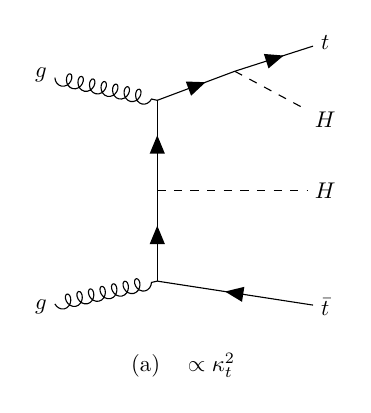
\begin{tikzpicture}[scale=0.82, transform shape]
\begin{feynman}
\vertex (i1) at (0,1.8) {\(g\)};
\vertex (i2) at (0,-1.8) {\(g\)};
\vertex (a) at (1.8,1.4);
\vertex (b) at (1.8,-1.4);
\vertex (h1) at (1.8,0);
\vertex (h2) at (3.0,1.85);
\vertex (f1) at (4.4,2.3) {\(t\)};
\vertex (f2) at (4.4,-1.8) {\(\bar t\)};
\vertex (H1) at (4.4,0.0) {\(H\)};
\vertex (H2) at (4.4,1.1) {\(H\)};
\diagram* {
 (i1) -- [gluon] (a),
 (i2) -- [gluon] (b),
 (f2) -- [fermion] (b) -- [fermion] (h1) -- [fermion] (a) -- [fermion] (h2) -- [fermion] (f1),
 (h1) -- [scalar] (H1),
 (h2) -- [scalar] (H2),
};
\end{feynman}
\node at (2.2,-2.7) {(a) 진폭 \(\propto \kappa_t^{2}\)};
\end{tikzpicture}\hspace{3mm}%
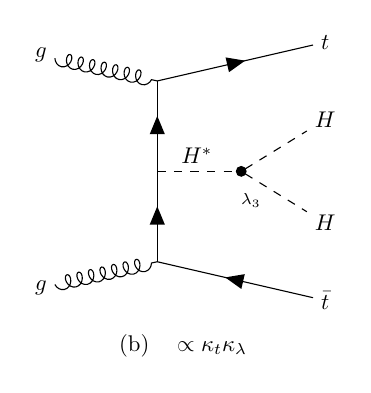
\begin{tikzpicture}[scale=0.82, transform shape]
\begin{feynman}
\vertex (i1) at (0,1.8) {\(g\)};
\vertex (i2) at (0,-1.8) {\(g\)};
\vertex (a) at (1.8,1.4);
\vertex (b) at (1.8,-1.4);
\vertex (h1) at (1.8,0);
\vertex [dot] (tri) at (3.1,0) {};
\vertex (f1) at (4.4,2.0) {\(t\)};
\vertex (f2) at (4.4,-2.0) {\(\bar t\)};
\vertex (H1) at (4.4,0.8) {\(H\)};
\vertex (H2) at (4.4,-0.8) {\(H\)};
\diagram* {
 (i1) -- [gluon] (a),
 (i2) -- [gluon] (b),
 (f2) -- [fermion] (b) -- [fermion] (h1) -- [fermion] (a) -- [fermion] (f1),
 (h1) -- [scalar, edge label=\(H^{*}\)] (tri),
 (tri) -- [scalar] (H1),
 (tri) -- [scalar] (H2),
};
\end{feynman}
\node at (3.25,-0.45) {\scriptsize\(\lambda_3\)};
\node at (2.2,-2.7) {(b) 진폭 \(\propto \kappa_t\kappa_\lambda\)};
\end{tikzpicture}\hspace{3mm}%
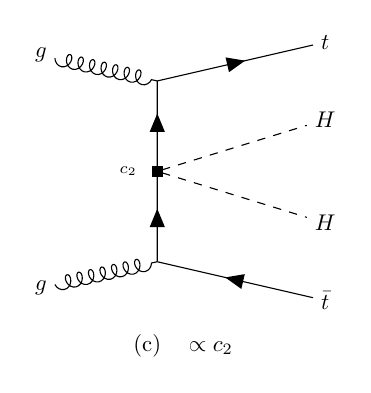
\begin{tikzpicture}[scale=0.82, transform shape]
\begin{feynman}
\vertex (i1) at (0,1.8) {\(g\)};
\vertex (i2) at (0,-1.8) {\(g\)};
\vertex (a) at (1.8,1.4);
\vertex (b) at (1.8,-1.4);
\vertex [square dot] (c) at (1.8,0) {};
\vertex (f1) at (4.4,2.0) {\(t\)};
\vertex (f2) at (4.4,-2.0) {\(\bar t\)};
\vertex (H1) at (4.4,0.8) {\(H\)};
\vertex (H2) at (4.4,-0.8) {\(H\)};
\diagram* {
 (i1) -- [gluon] (a),
 (i2) -- [gluon] (b),
 (f2) -- [fermion] (b) -- [fermion] (c) -- [fermion] (a) -- [fermion] (f1),
 (c) -- [scalar] (H1),
 (c) -- [scalar] (H2),
};
\end{feynman}
\node at (1.35,0.0) {\scriptsize\(c_2\)};
\node at (2.2,-2.7) {(c) 진폭 \(\propto c_2\)};
\end{tikzpicture}
\caption{\ttHH 의 대표 LO 도형(gg 시작, t-channel top 교환). (a) 두 Higgs 가 모두 top 선에서 방출된다(Yukawa 두 번). (b) top 선에서 나온
off-shell $H^{*}$ 가 삼중 결합 $\lambda_3$ 로 HH 가 된다. (c) HEFT 의 $t\bar tHH$ 접촉 꼭짓점(SM 에서는 $c_2=0$). 실제 도형은 이 밖에도 $q\bar q$ 시작,
s-channel gluon, Higgs 방출 위치가 다른 것들이 있다.}
\label{fig:intro-feyn}
\end{figure}

세 결합에 대한 의존성은 AN 의 HEFT 해석 식에 모여 있다\src{AN-22-122 v26, PDF p.127, Eq.~22}:
\begin{equation}
  \sigma_{\ttHH}(\kl,\kt,c_2) = \kt^{4}A + \kl^{2}\kt^{2}B + c_2^{2}C + \kt^{3}\kl D + \kt^{2}c_2E + \kl\kt c_2F .
  \label{eq:intro-heft}
\end{equation}
승인 발표는 $A$--$F$ 가 도형별 기여와 그 간섭이라 설명하고 Goertz et al.(JHEP04(2015)167)을 인용한다\src{승인 발표 p.34}. $A$--$F$ 의 값은 AN 에 없다(확인 못 함).

\begin{note}[도형과 HEFT 식의 여섯 항]
전체 진폭을 $\mathcal{M}=\kt^{2}\mathcal{M}_a+\kt\kl\,\mathcal{M}_b+c_2\,\mathcal{M}_c$ 로 쓰면 $|\mathcal{M}|^{2}$ 의 여섯 항이 그대로 식~\eqref{eq:intro-heft} 의
$A$($|\mathcal{M}_a|^2$), $B$($|\mathcal{M}_b|^2$), $C$($|\mathcal{M}_c|^2$), $D$(a–b 간섭), $E$(a–c 간섭), $F$(b–c 간섭)다. 따라서 \ttHH 에도 Yukawa 도형과
삼중 결합 도형 사이의 간섭항 $D\propto\kt^{3}\kl$ 은 있다. AN 의 "간섭항이 없다"는 문장은 ggF HH 처럼 SM 근처에서 두 도형이 크게 상쇄하는 일이
없다는 뜻으로 읽는 것이 맞다(우리 판단; 발표들의 "음의 간섭 없이"라는 표현과 일치한다). 표~\ref{tab:intro-heft} 의 벤치마크에서 $\kl=2,3$ 의
단면적이 SM 보다 크므로 $\kl>1$ 쪽에서는 $\sigma(\kl)-\sigma(1)=(\kl-1)\,[B(\kl+1)+D]>0$, 곧 $\kl^{2}$ 항의 증가가 간섭항보다 크다($\kt=1$, $c_2=0$).
세 값을 그대로 풀면 $B\approx0.02$, $D\approx-0.03$(fb, $\times$BR)이지만 값이 두 자리로 반올림되어 있어 $D$ 의 부호는 정해지지 않는다(우리 계산).
\end{note}

AN 은 HEFT 표본 여덟 개의 13\TeV 단면적$\times$BR(HH$\to$4b)을 표~\ref{tab:intro-heft} 처럼 준다. 오른쪽 열은 SM 대비 비로, 우리가 계산한 것이다.
\kl 을 두세 배로 바꿔도 단면적은 10--40\,\% 변하지만, \kt 를 두 배로 하면 12 배, $c_2=3$ 이면 16 배가 된다. 곧 \ttHH 는 일차적으로 \kt 와 $c_2$ 를
재는 과정이고 \kl 에는 약하게만 민감하다 — AN 의 "λ 에 대한 감도가 전반적으로 작다"는 문장의 정량적 내용이다(우리 판단).

\begin{table}[htbp]
\centering
\caption{AN 의 HEFT 벤치마크 표본: 13\TeV 단면적$\times\mathrm{BR}(HH\to4b)$, $\mathrm{BR}=0.5824^{2}$. 마지막 열은 SM(0.25\fb) 대비 비(우리 계산).}
\label{tab:intro-heft}
\small
\begin{tabular}{lccccc}
\toprule
표본(\texttt{TTHHTo4b\_HEFT\_...}) & $c_2$ & \kt & \kl & $\sigma\times$BR [fb] & SM 대비 \\
\midrule
SM (\texttt{TTHHTo4b})   & 0  & 1 & 1   & 0.25  & 1 \\
\texttt{kl-2}            & 0  & 1 & 2   & 0.28  & 1.12 \\
\texttt{kl-3}            & 0  & 1 & 3   & 0.35  & 1.40 \\
\texttt{kt-2}            & 0  & 2 & 1   & 3.11  & 12.4 \\
\texttt{kl-0p5\_c2-1}    & 1  & 1 & 0.5 & 0.72  & 2.88 \\
\texttt{c2-m1}           & $-1$ & 1 & 1 & 0.78  & 3.12 \\
\texttt{c2-3}            & 3  & 1 & 1   & 4.03  & 16.1 \\
\texttt{c2-6}            & 6  & 1 & 1   & 14.15 & 56.6 \\
\bottomrule
\end{tabular}
\par\smallskip\footnotesize 출처: AN-22-122 v26, PDF p.129, Table~58(같은 값: 승인 발표 p.34). Table~58 의 POSTFIX 는 \texttt{amcatnlo-pythia8} 인데
Tables~10--12 의 데이터셋 이름은 \texttt{madgraph-pythia8} 이다(AN 내부 불일치).
\end{table}

AN 의 HEFT 결합 상수 결과(SL 채널, Asimov)는 $c_2$ 하나를 움직인 scan 에서 기대 95\,\% CL $-5.0<c_2<4.8$\src{AN-22-122 v26, PDF p.127},
2 차원 우도에서 $c_2=0.00^{+4.13}_{-4.33}$, $\kl=1.00^{+8.64}_{-5.60}$((\(c_2,\kl\)) 평면), $\kt=1.00^{+0.30}_{-0.45}$((\(c_2,\kt\)) 평면)이다\src{AN-22-122 v26, PDF p.130, Fig.~102}.
\kl 하나만 움직이는 scan 은 AN 에 없다. 승인 발표의 최종(실데이터) 결과는 관측(기대) $-6.6<c_2<6.4$ ($-5.4<c_2<5.2$)다\src{승인 발표 p.35}.
AN 의 BSM 동기는 MCHM 의 top 부문, $T\to tH$ 로 붕괴하는 전하 2/3 vector-like quark 공명(쌍생성되면 \ttHH 말단 상태), 그리고 HEFT 의
$hhh$, $tthh$, $gghh$ 유효 꼭짓점이다\src{AN-22-122 v26, PDF p.8--11}. AN 의 목표는 렙톤 채널의 신호 세기 측정과 SL 채널의 HEFT 결합
연구다\src{AN-22-122 v26, PDF p.11, l.251--253}. FH 에서도 같은 해석을 나중에 할 수 있지만 지금 계획에는 신호 세기 상한이 먼저다\src{ROADMAP\_FH §1}.

% -----------------------------------------------------------------------------
\section{신호 정의: \texorpdfstring{\ttHH, \HHfourb, \ttbar}{ttHH, HH to 4b, ttbar} 완전 강입자 붕괴}\label{sec:intro-signal}

\subsection{단면적}\label{sec:intro-xsec}

AN 의 신호 단면적은 13\TeV 에서 $\sigma(\ttHH)=0.756\fb$, scale 불확도 $^{+4.3}_{-15.0}\%$, PDF$+\alpha_s$ $\pm3.4\%$(NLO QCD)다\src{AN-22-122 v26, PDF p.23, Table 9}.
신호 표본 \file{/TTHHTo4b_TuneCP5_13TeV-madgraph-pythia8/} 은 MadGraph5 2.6.5 의 LO 로 만들어졌고\src{AN-22-122 v26, PDF p.19, l.399--401},
AN 은 XSDB 의 LO 값 0.669\fb 에 k-factor 1.130 을 곱해 NLO 값으로 맞춘다($0.669\times1.130=0.756$)\src{AN-22-122 v26, PDF p.24, Table 10}.
14\TeV 값은 0.934\fb 다\src{AN-22-122 v26, PDF p.7, Table 1}.

우리 단면적 DB(\file{data/samples_2017UL.json}, \file{data/samples_2018UL.json})도 13\TeV 에 0.756\fb 를 쓰고 HH$\to$4b 분기비를 따로
곱한다\src{samples\_2017UL.json, TTHHto4b}. 2024(13.6\TeV)에는 \file{data/samples_2024.json} 이 $0.860\fb$(scale $^{+4.2}_{-14.0}\%$,
PDF$+\alpha_s$ $\pm3.3\%$, NLO QCD)를 쓰는데, 이 값은 우리 자료 가운데 이 DB 에만 있고 출처는 AI 가 2026-10-05 에 공개 자료에서 모은 ATLAS 논문
(arXiv:2603.13113)의 인용이다\src{samples\_2024.json, TTHHto4b}\src{STEP 24 §7}. DB 는 모든 2024 단면적을 PROVISIONAL 로 표시하고 그 값으로 만든
plot 에는 "provisional cross sections" 를 적게 한다\src{D-2026-10-05-A}. 13.6/13 의 비는 $0.860/0.756=1.138$ 이다.

\begin{openq}[신호 단면적: 세 값]
\begin{itemize}
  \item 승인 발표와 Wei Wei 의 DPF 발표는 $\sigma(\ttHH,13\TeV)=0.775\fb$($^{+1.5}_{-4.3}\%$, $\pm3.2\%$)를 쓰고\src{승인 발표 p.3, p.27}\src{Wei Wei, DPF 2026 p.2},
        같은 승인 발표의 표본 표와 사전승인 발표는 0.756\fb 를 쓴다\src{승인 발표 p.8}\src{사전승인 발표 p.3}. 우리 계산으로 $0.669\times1.158=0.775$ 이고, 우리 DB 의
        note 는 "AN Table~10 의 k-factor 1.158" 을 적어 두었다\src{samples\_2017UL.json, TTHHto4b}. 또 AN Table~10 의 "$0.669\fb\times0.5824^{2}=0.263\fb$" 는 산술이
        맞지 않고($0.669\times0.5824^2=0.227$) $0.775\times0.5824^2=0.263$ 과 같다. 두 값은 k-factor 1.130 과 1.158 의 차이로 보인다(우리 추정; AN 의 다른 판).
        승인 발표의 상한 37(42)\fb 는 $48.7\times0.756=36.8$, $55.3\times0.756=41.8$ 과 맞으므로 SL 의 최종 결과는 0.756\fb 를 썼다고 본다(우리 계산).
        \textbf{우리는 0.756\fb 를 쓴다.} 결합할 때 팀과 한 값으로 맞춰야 한다.
  \item 13.6\TeV 의 0.860\fb 는 CMS·LHC Higgs WG 의 공식 표가 아니다. 결과 전에 LHC Higgs WG(또는 GenXSecAnalyzer + 같은 차수의 k-factor)로 확인한다.
\end{itemize}
\end{openq}

\subsection{분기비와 붕괴 채널}\label{sec:intro-br}

AN 은 $\mathrm{BR}(\Hbb)=0.5824$, $\mathrm{BR}(W\to\mathrm{had})=0.6741$, $\mathrm{BR}(W\to\ell\nu)=0.3259$, $\mathrm{BR}(Z\to\bbbar)=0.15$ 를 쓴다\src{AN-22-122 v26, PDF p.38, Table 25}.
따라서 $\mathrm{BR}(\HHfourb)=0.5824^{2}=0.33918976$ 이고, 이것이 우리 DB 의 신호 \code{br} 값이다\src{samples\_2017UL.json, TTHHto4b}. \ttbar 의 붕괴는
$W\to\ell\nu$ 를 $1-0.6741$ 로 정의해(τ 포함) 세 채널로 나눈다. 우리 코드는 이 값을 \file{compute_stitch_factors.py} 의 \code{W_HAD}$\,=0.6741$,
\code{BR_HAD}$\,=$\,\code{W_HAD}$^{2}$ 에서 쓰고\src{compute\_stitch\_factors.py, l.168--172}, 같은 수가 DB 의 \file{TTbar_*}·\file{TTbb_*} 의 \code{br} 에 있다.
2024 DB 는 $W\to\mathrm{had}=0.6741$ 의 출처를 PDG 2024($67.41\pm0.27\,\%$)로 적었다\src{samples\_2024.json, \_meta}.

\begin{table}[htbp]
\centering
\caption{\ttbar 붕괴 채널과 신호의 전체 분기 비율. 가운데 두 열은 우리 코드의 값과 그것에 $\mathrm{BR}(\HHfourb)$ 를 곱한 값(우리 계산).}
\label{tab:intro-br}
\small
\begin{tabularx}{\textwidth}{l c c c L}
\toprule
채널 & W 붕괴 & $\mathrm{BR}(\ttbar\to\cdot)$ & $\times\,0.33919$ & 발표·AN 의 표기 \\
\midrule
FH & 둘 다 $q\bar q'$ & $0.6741^{2}=0.45441$ & 0.1541 & "largest top-pair branching (≈46\,\%)"\src{Hbb 회의 FH 발표 p.8} \\
SL & 하나 $\ell\nu$  & $2\times0.6741\times0.3259=0.43938$ & 0.1490 & 11.4\,\%\src{AN-22-122 v26, PDF p.5, l.65}\src{승인 발표 p.6} \\
DL & 둘 다 $\ell\nu$ & $0.3259^{2}=0.10621$ & 0.0360 & "about 4.2\,\%"\src{AN-22-122 v26, PDF p.5, l.69}; 3.6\,\%\src{사전승인 발표 p.5} \\
\bottomrule
\end{tabularx}
\end{table}

AN·발표의 SL 11.4\,\% 와 DL 4.2\,\%(또는 3.6\,\%)의 정확한 정의(τ 를 어떻게 셌는지)는 쓰여 있지 않다(확인 못 함). 우리 정의로는 DL 이 3.6\,\% 로
사전승인 값과 맞고 SL 은 14.9\,\% 로 11.4\,\% 와 맞지 않는다. FH 의 분기 비율은 우리 정의로 $0.45441\times0.33919=15.4\,\%$ 이다(우리 계산).

\begin{note}[신호 표본에는 모든 \ttbar 붕괴가 들어 있다]
AN 의 표본은 \ttH(bb) 와 \ttbar 만 SL·DL 전용이고 나머지는 \ttbar 붕괴에 대해 inclusive 다\src{AN-22-122 v26, PDF p.21, l.420--422}
(원문은 ``except ttH(bb), tt, and ttH(bb)'' 로 \ttH(bb) 를 두 번 적었는데, 4FS \ttbb 표본도 SL·DL 전용이다\src{AN-22-122 v26, PDF p.28, Table 15}). 우리 신호 표본
\file{TTHHto4b} 도 마찬가지라 FH 선택(렙톤 veto)에는 FH 붕괴뿐 아니라 렙톤을 놓친 SL·DL 사건, $\tau_h$ 를 가진 사건도 들어온다. 우리는 이것을 모두 신호로
센다. FH 채널은 붕괴 채널이 아니라 \emph{재구성된} 렙톤 수(0 개)로 정의되므로, SL·DL 과 결합할 때 직교성은 세 채널의 렙톤 정의가 서로 맞물리는지로
보장해야 한다(우리 판단; 렙톤 정의는 \ref{ch:objects}~장).
\end{note}

\subsection{FH 말단 상태와 조합 문제}\label{sec:intro-combinatorics}

FH 의 LO 말단 상태는 HH 에서 b 쿼크 4 개, 두 top 에서 b 쿼크 2 개, 두 W 에서 가벼운 쿼크 4 개, 모두 10 개의 쿼크이고 중성미자가 없어 원리적으로
완전히 재구성할 수 있다\src{Hbb 회의 FH 발표 p.8}\src{KCMS 발표 p.2}. 실제로는 FSR 이 jet 을 늘리고, 가까운 쿼크가 한 jet 으로 합쳐지고, 일부는
acceptance 밖으로 나가므로 jet 수는 사건마다 다르다. ttH(bb) FH 는 이 때문에 7, 8, $\geq9$ jet 범주를 썼고\src{AN-19-094 v20, PDF p.99--100},
우리 SR 계획도 $n_b\geq4$, $n_{\mathrm{jets}}$ 범주 7/8/$\geq9$, Higgs 후보 질량창(예: $100<m(H_1),m(H_2)<140\GeV$)에서 출발한다\src{Hbb 회의 FH 발표 p.14}.
SL 의 경우 AN 은 "LO 에서 8 개의 jet, 그중 6 개 이상 b-tag" 라고 쓴다\src{AN-22-122 v26, PDF p.5, l.63--65}.

jet 을 부모 입자에 배정하는 경우의 수가 FH 재구성의 핵심 문제다. 10 개의 jet 을 (b, $q\bar q'$)인 top 둘과 b 쌍인 Higgs 둘에 배정하는 서로 다른 방법은
\begin{equation}
  N_{\mathrm{assign}} = \frac{10!}{2^{4}\cdot2\cdot2} = 56\,700
  \label{eq:intro-comb}
\end{equation}
이다($2^4$: 네 쌍 안의 순서, $2\cdot2$: 두 top 과 두 Higgs 의 맞바꿈; 우리 계산). b-tag 이 완벽해 6 개의 b jet 과 4 개의 가벼운 jet 을 안다고 해도
$\binom{6}{2}\cdot3\cdot3\cdot2=270$ 가지가 남고, Higgs 두 개만 고를 때도 b-tag jet 6 개에서 $\binom{6}{4}\cdot3=45$ 가지다(우리 계산). AN 은 이 문제를 HH·ZZ·ZH
가설의 \chisq 쌍 짓기, SL 의 jet-assignment BDT(JABDT), DL 의 graph-attention 할당(GATJA)으로 풀었다(\ref{ch:reco}·\ref{ch:mva}~장).

\subsection{생성 사건 수 어림}\label{sec:intro-yield}

표~\ref{tab:intro-yield} 는 선택 전에 생성되는 신호 사건 수 $N=\sigma\cdot\mathrm{BR}\cdot L$ 의 어림이다\,\tagours. Run~2 의 루미노시티는 AN 의 연도별 값을,
2017·2018 은 우리 정규화 값도 함께 적었다(루미노시티의 출처와 차이는 \ref{ch:samples}~장). 2024 는 13\TeV 단면적과 13.6\TeV 임시 단면적 둘로 계산했다.

\begin{table}[htbp]
\centering
\caption{생성되는 신호 사건 수의 어림(선택 전; 우리 계산). $\sigma\cdot\mathrm{BR}_{4b}=\sigma\times0.33919$ 는 모든 \ttbar 붕괴, $N_{\mathrm{FH}}$ 는 여기에 0.45441 을 곱한 것.}
\label{tab:intro-yield}
\small
\begin{tabular}{l c c c c}
\toprule
기간 & $L$ [\fbinv] & $\sigma$ [fb] & $\sigma\cdot\mathrm{BR}_{4b}\cdot L$ & $N_{\mathrm{FH}}$ \\
\midrule
2016 (AN)        & 36.31  & 0.756 & 9.3  & 4.2 \\
2017 (AN / 우리) & 41.53 / 42.07 & 0.756 & 10.6 / 10.8 & 4.8 / 4.9 \\
2018 (AN / 우리) & 59.74 / 59.56 & 0.756 & 15.3 / 15.3 & 7.0 / 6.9 \\
Run~2 (AN)       & 137.60 & 0.756 & 35.3 & 16.0 \\
2024 C--I        & 109.816 & 0.756 (13\TeV) & 28.2 & 12.8 \\
2024 C--I        & 109.816 & 0.860 (13.6\TeV, 임시) & 32.0 & 14.6 \\
\bottomrule
\end{tabular}
\par\smallskip\footnotesize 입력: $L$ — AN-22-122 v26, PDF p.19, Table~4; LUMI\_SOURCES §2, §6. $\sigma$ — AN Table~9; samples\_2024.json.
\end{table}

Run~2 와 2024 를 합쳐도 FH 로 붕괴하는 신호는 약 30 개(28.8--30.6 개) 생성된다. 우리 결정 기록도 같은 어림(2017 에 약 11 개, 2024 에 약 28 개, 모든 \ttbar 붕괴)을
blinding 정책의 근거로 썼다\src{D-2026-10-02-E}. 2017 의 첫 cut-flow 에서 baseline 뒤 신호는 4.3 개였고 같은 선택의 MC 배경은 $3.39\times10^{6}$ 개였다
\src{Hbb 회의 FH 발표 p.25}: $S/B\approx1.3\times10^{-6}$(우리 계산). 발표들이 인용하는 "Run~3 에 약 400 개, HL-LHC 에 약 3000 개"\src{사전승인 발표 p.3}\src{승인 발표 p.3}는
분기비를 곱하기 전의 생성 수로 보인다(우리 판단: $3000\fbinv\times$ 약 $1\fb$, 발표에는 정의가 없다).

% -----------------------------------------------------------------------------
\section{연구 현황: 우리 자료가 말하는 것}\label{sec:intro-status}

\subsection{SL·DL 결과}

표~\ref{tab:intro-results} 는 우리 자료에 있는 \ttHH(4b) 결과를 모은 것이다. 모두 신호 세기 $\mu=\sigma/\sigma_{\mathrm{SM}}$ 에 대한 95\,\% CL 상한이다.
AN v26 의 결과는 모두 Asimov(blind)이고 실데이터 결과 절(§9)은 비어 있다\src{AN-22-122 v26, PDF p.138}. 사전승인(2025-04-15) 때는 SL·DL 결합이 대상이었지만,
승인(2026-07)은 SL 단독이었다("SL preapproved, SL ARC Green Light")\src{승인 발표 p.2}.

\begin{table}[htbp]
\centering
\caption{우리 자료의 \ttHH(\HHfourb) 결과(95\,\% CL 상한, $\times$SM). "기대" 는 신호가 없을 때의 중앙값.}
\label{tab:intro-results}
\small
\begin{tabularx}{\textwidth}{l l c c L}
\toprule
시점·자료 & 채널(데이터) & 기대 & 관측 & 비고 \\
\midrule
AN v26 (Asimov) & SL, Run~2 & 46.5 & — & stat 만 39.0\src{AN-22-122 v26, PDF p.127, Table 57} \\
                & DL, Run~2 & 34.63 & — & stat 만 28.63\src{AN-22-122 v26, PDF p.133, Tables 65--66} \\
                & SL+DL     & 25.13 & — & $\hat\mu=1.0^{+11.68}_{-7.96}$\src{AN-22-122 v26, PDF p.137, Table 67} \\
사전승인 (2025-04) & SL / DL / 결합 & 42.5 / 34.63 / 25.13 & — & "통계 불확도가 지배"\src{사전승인 발표 p.25--26} \\
2차 ARC (2025-12, \ttbar 하나) & SL, Run~2 & 50.5 & 79.3 & \src{승인 발표 p.29} \\
승인 최종 (\ttbar 와 $t\bar tb$ 분리) & SL, Run~2 & 55.3 & 48.7 & $\sigma$ 로 기대 42, 관측 37\fb\src{승인 발표 p.32--33}\src{Wei Wei, DPF 2026 p.12} \\
HL-LHC 예측 (FTR-21-010) & SL, 3000\fbinv & 3.14 & — & \src{승인 발표 p.5} (그림 판독) \\
\bottomrule
\end{tabularx}
\end{table}

두 가지가 눈에 띈다. 첫째, SL 의 기대 상한이 사전승인 42.5 에서 최종 55.3 으로 약 30\,\% 나빠졌다(우리 계산); 그 사이에 ARC 와 \ttbar 배경을
\ttbar(lf, cc)와 $t\bar tb$(mb, nb) 두 template 로 나누고 ttH·\ttbar·$t\bar tb$ 의 정규화를 자유 변수로 두는 fit 모형이 채택되었다\src{승인 발표 p.25, p.27, p.30--32}.
원인 설명은 슬라이드에 없다. 둘째, 결합 기대 상한 25.13 에서 stat 만이면 23.19 라서\src{사전승인 발표 p.25} 이 분석은 통계 지배다 —
채널을 늘리는 것(FH)이 곧 감도를 늘리는 길이다(우리 판단).

\subsection{FH 채널의 자리}

AN 에서 FH 는 한 문장뿐이다: "The hadronic decay of the top pair is under study as well and the object of another Analysis Note, in progress."
\src{AN-22-122 v26, PDF p.5, l.58--60}. 사전승인·승인·Wei Wei 발표에는 FH 언급이 없다. 우리 발표는 FH 를 "같은 분석팀이 HIG-24-016,
AN-2022/122 의 보완 채널로 개발한다"고 했고\src{Hbb 회의 FH 발표 p.5}, KCMS 에서는 "HIG-24-016 SL/DL 논문의 후속(follow-up) FH 결과"를 목표로
적었다\src{KCMS 발표 p.4}. SL·DL 과의 결합은 "채널들이 양립 가능하다고 판명되면" 이라는 조건부다\src{Hbb 회의 FH 발표 p.38}. FH 가 더하는 것은 가장
큰 \ttbar 분기 비율, 중성미자 없는 완전 재구성, SL·DL 과의 통계적 독립이고, 대가는 QCD multijet 이 지배적 배경이 되는 것이다\src{Hbb 회의 FH 발표 p.6, p.8}.

\subsection{참고: ttH(bb) FH 의 감도}

ttH(bb) 의 full Run~2 분석은 FH 채널이 무엇을 줄 수 있는지에 대한 가장 가까운 선례다. FH 단독 fit 의 Asimov 결과는
$\mu=1.00^{+0.77}_{-0.78}$(stat $\pm0.23$), 기대 유의도 1.3σ 로, 같은 분석의 DL 1.9σ, SL 3.0σ, 결합 4.1σ 와 비교된다\src{AN-19-094 v20, PDF p.243, Table 129}.
FH 는 tt+B, tt+C 정규화에 대한 감도가 거의 없어 FH 단독 fit 에서는 이 둘을 50\,\% lnN 으로 묶었고, 채널 사이에 nuisance 를 상관시킨 fit 에서는
FH 의 불확도가 $^{+0.44}_{-0.41}$ 로 줄었다\src{AN-19-094 v20, PDF p.243--244, Fig.~134}. 관측값은 FH 단독 $\mu=-1.31^{+0.82}_{-0.89}$ 였다\src{AN-19-094 v20, PDF p.243, Table 130}.
SR 의 사전(pre-fit) $S/B$ 와 $S/\sqrt{B}$ 는 Run~2 에서 7 jet 0.0056/1.47, 8 jet 0.0069/1.93, $\geq9$ jet 0.0087/2.14 로 jet 이 많은 범주가 가장 민감했다
\src{AN-19-094 v20, PDF p.587, Fig.~503}.

\begin{note}[ttH(bb) FH 에서 \ttHH FH 로 옮겨 읽기]
\ttH 의 FH 는 단독으로는 DL 보다 약간 약했고, 결합에서 nuisance(특히 tt+B)가 다른 채널로 제약될 때 제 몫을 했다. \ttHH FH 도 같은 구조일
가능성이 크다: FH 단독 결과는 \ttbb 정규화 가정에 크게 좌우될 것이므로 SL·DL 과의 결합 또는 다른 제약이 필요하다\src{ROADMAP\_FH §7}.
한편 \ttHH 는 \ttH 보다 b 쿼크가 두 개 많아 SR 을 더 높은 b 다중도에 둘 수 있고, 그 영역에서는 QCD 와 \ttbar+light 가 더 줄어든다. 반대로
QCD 추정의 외삽 거리는 길어진다(\ref{ch:qcd}~장). 이 둘 가운데 무엇이 이길지는 아직 모른다(우리 판단).
\end{note}

% -----------------------------------------------------------------------------
\section{FH 가 어려운 이유와 이 분석이 풀어야 할 것}\label{sec:intro-challenges}

\paragraph{QCD multijet.} 렙톤도 \MET 도 요구하지 않으므로 강한 상호작용의 다중 jet 생성이 압도적이다. ttH(bb) FH 의 baseline 에서 2017 QCD(MC)는
$3.27\times10^{6}$, 전체 배경은 $3.89\times10^{6}$, ttH 는 2649 개였다\src{AN-19-094 v20, PDF p.70, Table 56}: QCD 가 84\,\%, $S/B\approx7\times10^{-4}$(우리 계산).
SR 에서도 QCD 가 80\,\% 이상이었고\src{AN-19-094 v20, PDF p.100, l.1118}, QCD MC 는 모양과 정규화 모두 잘 맞지 않아 초기 연구에만 쓰였다
\src{AN-19-094 v20, PDF p.68, l.706--709}. 우리 2017 첫 cut-flow 도 baseline MC $3.39\times10^{6}$ 가운데 QCD 가 $2.60\times10^{6}$ 였고, b-tag 수가 늘수록
Data/MC 가 커졌다\src{Hbb 회의 FH 발표 p.25--26}. 2024 에서도 SF 없이 본 FH 의 Data/MC 는 1.40(nb $\geq3$ 2.02, $\geq4$ 2.18)이고 MC 의 78\,\% 가
LO QCD 다\src{STATUS 2026-10-09 (3)}. 그래서 QCD 는 데이터에서 추정한다(\ref{ch:qcd}~장).

\paragraph{trigger.} 렙톤 trigger 를 쓸 수 없어 $\HT$, 다중 jet, online b-tag 을 조합한 trigger 를 쓴다(2017: 6 jet+1 b, 6 jet+2 b, 4 jet+3 b,
\code{HLT_PFHT1050})\src{Hbb 회의 FH 발표 p.15}. 오프라인 문턱($\HT>500\GeV$, 6 번째 jet $\pt>40\GeV$)이 turn-on 근처라 trigger SF 를 $(\HT, p_{\mathrm T}^{j6})\times n_b$
에서 따로 잰다\src{Hbb 회의 FH 발표 p.16}. 2024 에는 b-tag 경로가 \file{ParkingHH} PD 에만 기록되어 PD 규칙이 바뀌었다\src{D-2026-10-06-A}(\ref{ch:trigger}~장).

\paragraph{\ttbar+heavy flavour.} 추가 b jet 을 가진 \ttbar, 특히 tt+bb 와 tt+$\geq$3b 는 신호와 같은 말단 상태라 줄일 수 없는(irreducible) 배경이다.
AN 은 \ttH 에서 중요했던 tt+bb 에 더해 tt+4b 가 \ttHH 에서 중요하다고 쓴다\src{AN-22-122 v26, PDF p.5--6, l.94--97}. 이 배경의 모델링과 5FS·4FS·tt4b 표본의
stitching 은 \ref{ch:samples}~장.

\paragraph{조합과 높은 b-tag 다중도.} 식~\eqref{eq:intro-comb} 의 조합 수 때문에 질량 재구성이 흐려지고, $n_b\geq4$ 영역에서는 c·light jet 의 mistag 과
b-tag SF 의 외삽이 중요해진다(\ref{ch:btag}·\ref{ch:reco}~장).

표~\ref{tab:intro-handles} 는 이 어려움과 그것을 다루는 수단, 그리고 해당 장을 짝지은 것이다.

\begin{table}[htbp]
\centering
\caption{FH 의 어려움과 다루는 수단.}
\label{tab:intro-handles}
\small
\begin{tabularx}{\textwidth}{>{\raggedright\arraybackslash}p{3.0cm} L >{\raggedright\arraybackslash}p{1.5cm}}
\toprule
어려움 & 수단(선례 또는 계획) & 장 \\
\midrule
QCD multijet & b-tag 영역(TR/CR/SR)과 $m_{qq}$ 창으로 데이터에서 모양을 얻고 정규화는 fit 에서 자유(ttH FH 방법); DNN 의 QCD class; 렙톤 CR 로 MC 배경 점검 & \ref{ch:qcd}, \ref{ch:mva} \\
다중 jet trigger & 직교 단일 µ 영역에서 $(\HT,p_{\mathrm T}^{j6})\times n_b$ 의 trigger SF; 연도별 PD 규칙 & \ref{ch:trigger} \\
\ttbar+HF & 5FS \ttbar, 4FS \ttbb, LO tt4b 의 stitching; tt+mb·tt+nb DNN 노드; tt+B 자유 정규화 & \ref{ch:samples}, \ref{ch:stats} \\
조합 & HH/ZH/ZZ \chisq 쌍 짓기, jet–parton 할당(JABDT/GATJA 의 FH 판), W·top 질량 & \ref{ch:reco}, \ref{ch:mva} \\
높은 b-tag 다중도 & Run~2 shape SF + 정규화 재가중, 2024 fixed-WP(method 1a); 진짜 b 수별 closure & \ref{ch:btag} \\
낮은 $S/B$ & 다중 분류 DNN(AN 의 9 노드 + QCD), event shape, binned likelihood fit & \ref{ch:mva}, \ref{ch:stats} \\
\bottomrule
\end{tabularx}
\end{table}

% -----------------------------------------------------------------------------
\section{분석 사슬 개관}\label{sec:intro-chain}

그림~\ref{fig:intro-chain} 은 NanoAOD 에서 fit 까지의 사슬이다. 상자의 색은 2026-10-10 의 상태다. 아래 설명의 이름은 저장소의 실제 파일과
모드 이름이다\src{README §1, §8}\src{ROADMAP\_FH §2}.

\begin{figure}[htbp]
\centering
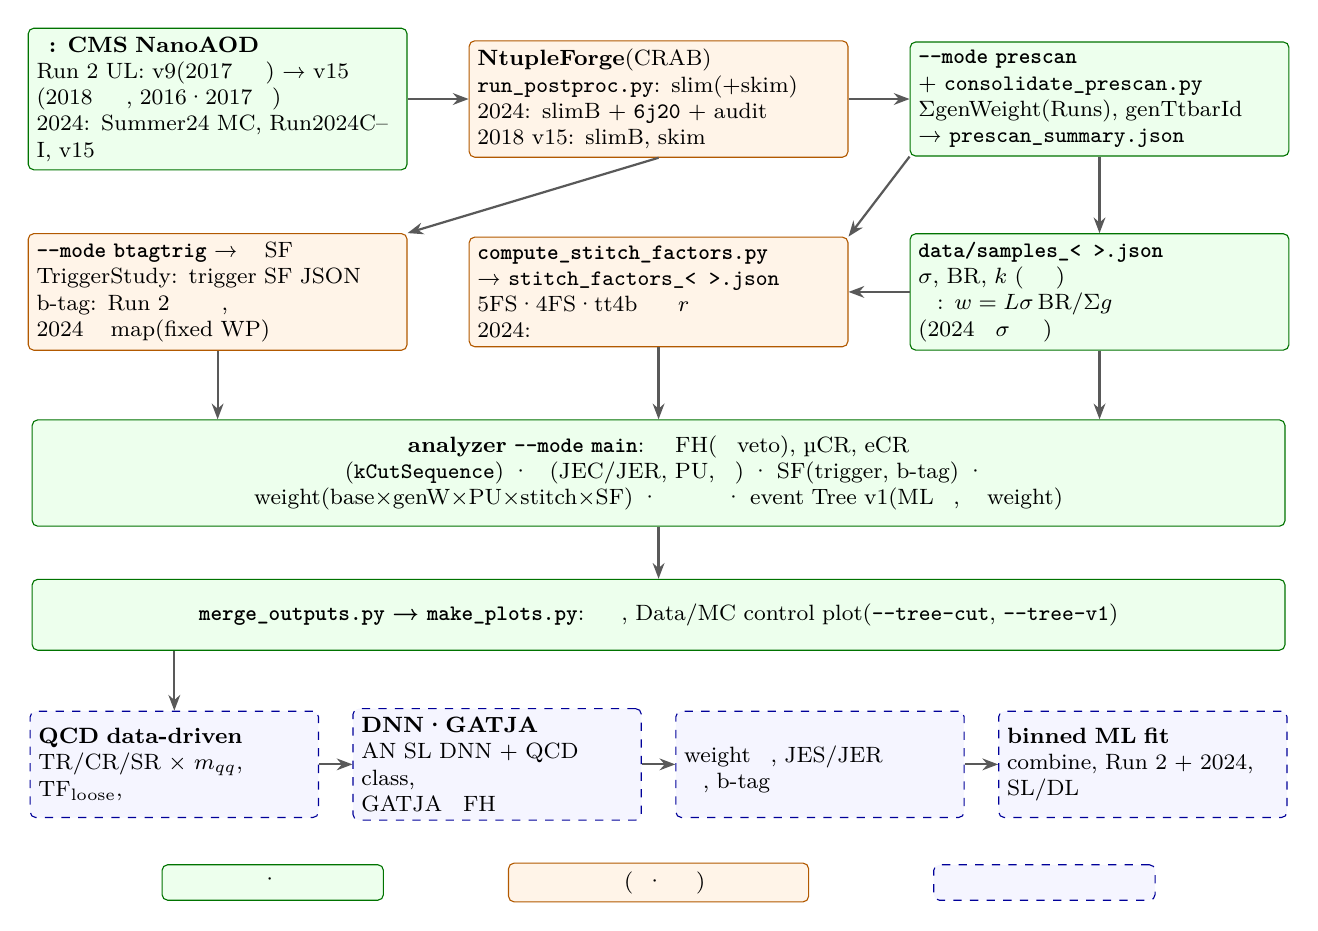
\begin{tikzpicture}[
  font=\footnotesize,
  >={Stealth[length=2mm]},
  base/.style={draw, rounded corners=2pt, align=left, inner sep=3pt, minimum height=1.35cm},
  done/.style={base, fill=green!7, draw=green!45!black},
  part/.style={base, fill=orange!9, draw=orange!70!black},
  plan/.style={base, fill=blue!4, draw=blue!60!black, dashed},
  ar/.style={->, thick, gray!70!black}
]
% 1 행
\node[done, text width=4.6cm] (nano) at (2.5,0) {\textbf{입력: CMS NanoAOD}\\
  Run~2 UL: v9(2017 첫 결과) → v15\\(2018 생산 끝, 2016·2017 계획)\\
  2024: Summer24 MC, Run2024C--I, v15};
\node[part, text width=4.6cm] (forge) at (8.1,0) {\textbf{NtupleForge}(CRAB)\\
  \texttt{run\_postproc.py}: slim(+skim)\\
  2024: slimB + \texttt{6j20} + audit\\
  2018 v15: slimB, skim 없음};
\node[done, text width=4.6cm] (pre) at (13.7,0) {\textbf{\texttt{--mode prescan}}\\
  + \texttt{consolidate\_prescan.py}\\
  $\Sigma$genWeight(Runs), genTtbarId 분할\\
  → \texttt{prescan\_summary.json}};
% 2 행
\node[part, text width=4.6cm] (bt) at (2.5,-2.45) {\textbf{\texttt{--mode btagtrig}} → 파생 SF\\
  TriggerStudy: trigger SF JSON\\
  b-tag: Run~2 정규화 재가중,\\ 2024 효율 map(fixed WP)};
\node[part, text width=4.6cm] (stitch) at (8.1,-2.45) {\textbf{\texttt{compute\_stitch\_factors.py}}\\
  → \texttt{stitch\_factors\_<연도>.json}\\
  5FS·4FS·tt4b 의 배수 $r$\\
  2024: 아직 없음};
\node[done, text width=4.6cm] (db) at (13.7,-2.45) {\textbf{\texttt{data/samples\_<연도>.json}}\\
  $\sigma$, BR, $k$ (단일 출처)\\
  제출기: $w=L\sigma\,\mathrm{BR}/\Sigma g$\\
  (2024 의 $\sigma$ 는 임시)};
% 3 행
\node[done, text width=15.7cm, align=center] (main) at (8.1,-4.75) {\textbf{analyzer \texttt{--mode main}}: 영역 FH(렙톤 veto), µCR, eCR\\
  선택(\texttt{kCutSequence}) · 보정(JEC/JER, PU, 청소) · SF(trigger, b-tag) · weight(base$\times$genW$\times$PU$\times$stitch$\times$SF)
  · 영역 히스토그램 · event Tree v1(ML 입력, 계통 weight)};
% 4 행
\node[done, text width=15.7cm, align=center, minimum height=0.9cm] (plot) at (8.1,-6.55) {\textbf{\texttt{merge\_outputs.py} → \texttt{make\_plots.py}}:
  수율 표, Data/MC control plot(\texttt{--tree-cut}, \texttt{--tree-v1})};
% 5 행 (계획)
\node[plan, text width=3.45cm] (qcd) at (1.95,-8.45) {\textbf{QCD data-driven}\\ TR/CR/SR $\times$ $m_{qq}$,\\ TF\textsubscript{loose}, 자유 정규화};
\node[plan, text width=3.45cm] (ml) at (6.05,-8.45) {\textbf{DNN·GATJA}\\ AN SL DNN + QCD class,\\ GATJA 의 FH 판};
\node[plan, text width=3.45cm] (syst) at (10.15,-8.45) {\textbf{계통 불확도}\\ weight 변형, JES/JER\\ 재실행, b-tag 변형};
\node[plan, text width=3.45cm] (fit) at (14.25,-8.45) {\textbf{binned ML fit}\\ combine, Run~2 + 2024,\\ SL/DL 과 결합};
% 화살표
\draw[ar] (nano) -- (forge);
\draw[ar] (forge) -- (pre);
\draw[ar] (forge.south) -- (bt.north east);
\draw[ar] (pre.south west) -- (stitch.north east);
\draw[ar] (pre) -- (db);
\draw[ar] (db) -- (stitch);
\draw[ar] (bt.south) -- (bt.south |- main.north);
\draw[ar] (stitch.south) -- (stitch.south |- main.north);
\draw[ar] (db.south) -- (db.south |- main.north);
\draw[ar] (main) -- (plot);
\draw[ar] (plot.south -| qcd.north) -- (qcd.north);
\draw[ar] (qcd) -- (ml);
\draw[ar] (ml) -- (syst);
\draw[ar] (syst) -- (fit);
% 범례
\node[done, minimum height=0.45cm, text width=2.6cm, align=center] (l1) at (3.2,-9.95) {구현·실행됨};
\node[part, minimum height=0.45cm, text width=3.6cm, align=center] (l2) at (8.1,-9.95) {일부(연도·기능 일부)};
\node[plan, minimum height=0.45cm, text width=2.6cm, align=center] (l3) at (13.0,-9.95) {계획};
\end{tikzpicture}
\caption{ttHH(4b) FH 분석 사슬과 2026-10-10 의 상태. 위 두 줄은 입력과 정규화·파생 보정, 가운데는 본 분석, 아래 줄은 아직 계획인 단계다.}
\label{fig:intro-chain}
\end{figure}

\begin{description}[leftmargin=0pt, labelsep=0.5em, itemsep=0.4ex]
  \item[입력과 생산.] NanoAOD 를 NtupleForge 가 CRAB 으로 slim(쓰지 않는 branch 제거)하고, 2024 는 저장된 \code{Jet_pt}$>20\GeV$·$|\eta|<2.5$ jet 6 개 이상
    (\code{6j20})으로 skim 한다\src{NtupleForge D-2026-09-28-volume}. 출력은 \file{forgedNtuple_<N>.root} 이고 \code{Runs} tree 는 skim 전 전체를 갖는다.
    2018UL·2024 v15 와 2024 ParkingHH 생산은 끝났고, 2016·2017 v15 hadronic 생산은 아직이며 Run~2 v15 에는 신호와 일부 배경이 중앙에 없다\src{ROADMAP\_FH §2, W3}
    (\ref{ch:samples}~장). 2017 의 첫 결과는 v9(\file{ttHH2017UL_fullNano_v20}) 위에서 나왔고 그 ntuple 은 KNU 에서 지워졌다\src{D-2026-10-05-D}\,\tagimpl.
  \item[정규화 입력.] analyzer 의 \texttt{-{}-mode prescan} 이 표본마다 $\Sigma$genWeight 와 genTtbarId 별 합을 모으고 \file{consolidate_prescan.py} 가 점검·집계한다.
    단면적·분기비는 \file{data/samples_<year>.json} 하나에서만 읽는다\src{STEP 11}. 제출기가 base weight 를 만들고, \file{compute_stitch_factors.py} 가 같은 DB 로
    stitching 배수를 만든다(\ref{ch:samples}~장)\,\tagimpl.
  \item[파생 보정.] \texttt{-{}-mode btagtrig} 의 skim 으로 TriggerStudy 가 trigger SF 를(2024 판 코드 끝\src{STEP 26}), Run~2 는 b-tag 정규화 재가중을,
    2024 는 fixed-WP b-tag 용 MC 효율 map(\file{tools/stage7/btag_eff_maps.py})을 만든다\src{STEP 25}. 2024 btagtrig 는 2026-10-10 에 도는 중이다\src{ROADMAP\_FH §2}\,\tagtest.
  \item[본 분석.] \texttt{-{}-mode main} 이 선택(선언적 표 \code{kCutSequence}; baseline 은 ttH FH 의 $n_{\mathrm{jets}}\geq6$, $p_{\mathrm T}^{j6}>40\GeV$, $\HT>500\GeV$,
    $n_b\geq2$, 렙톤 veto, $30<m_{qq}<250\GeV$)\src{README §5}, 보정과 SF, weight, 영역 히스토그램과 event tree 를 쓴다(\ref{ch:selection}~장). 영역은 FH 와 두 렙톤 CR
    (렙톤 하나 + $\MET>20\GeV$)이다\src{STEP 14}. Tree v1 이 DNN·GATJA 입력과 계통 weight 를 갖는다\src{STEP 27}(부록~\ref{ch:treev1})\,\tagimpl.
  \item[계획.] QCD data-driven(ttH FH 방법; 렙톤 CR 의 Data/MC 가 합리적인 뒤)\src{D-2026-10-10-B}, AN 의 SL DNN 을 FH 에 맞춘 다중 분류와 GATJA 의 FH 판
    \src{PLAN\_ML\_SYST §9}, 계통 불확도(\ref{ch:syst}~장)와 combine fit(\ref{ch:stats}~장)은 아직 계획이다\,\tagplan. 일정은 2026 하반기 full Run~2 확장과 QCD 방법 확립, 2027 상반기 DNN·SR 최적화·계통·fit 이다
    \src{KCMS 발표 p.4}(현황과 계획은 \ref{ch:status}·\ref{ch:plan}~장).
\end{description}

\begin{impl}
\begin{itemize}
  \item 분석기: \file{ttHHanalyzer_unified.cc}(모드, \code{kCutSequence}, weight 조립), \file{include/SelectionCuts.h}(cut 상수), \file{include/EraConfig.h}(연도 상수).
  \item 정규화: \file{submit_job_FH_Tier3_unified.py} 의 \code{_compute_base_weight}, \file{consolidate_prescan.py}, \file{compute_stitch_factors.py}.
  \item 파생 보정: \file{TriggerStudy/}(\code{run_analysis.sh}, DeriveSF), \file{bTagSF_ReweightStudy/}(Run~2), \file{tools/stage7/btag_eff_maps.py}(2024).
  \item 출력 처리: \file{outputMerger/merge_outputs.py}, \file{plotter/make_plots.py}. 작업 흐름과 의존성: \file{docs/ROADMAP_FH.md}.
\end{itemize}
\end{impl}

\begin{openq}[1 장의 미결 사항]
\begin{enumerate}
  \item 신호 단면적의 기준값(0.756 대 0.775\fb, \S\ref{sec:intro-xsec})과 13.6\TeV 값(0.860\fb, 임시)의 공식 출처 — 팀·LHC Higgs WG 확인.
  \item FH 결과의 문서 경로: 같은 AN(AN-2022/122)의 보완 채널인가, 별도 AN·후속 결과인가 — 두 발표의 표현이 다르다\src{Hbb 회의 FH 발표 p.5}\src{KCMS 발표 p.4}. 팀(Hbb 컨비너) 결정.
  \item 신호의 정의: TTHHto4b 의 비-FH 붕괴(렙톤을 놓친 SL·DL, $\tau_h$)를 FH 신호로 세는 것은 결합 때 채널 직교성과 함께 정해야 한다.
  \item SR 정의($n_b$, $n_{\mathrm{jets}}$ 범주, Higgs 질량창)는 아직 연구 전이다\src{Hbb 회의 FH 발표 p.14}. Hbb 발표 p.14 는 baseline 을 "AN-2022/122 Tab.~55" 로 적었으나
        그 baseline 은 AN-19-094 의 Table~55 다\src{README §5}.
  \item HEFT 해석(\kl, \kt, $c_2$)을 FH 에서도 할지 — 지금 계획(ROADMAP)은 신호 세기 상한이 먼저다.
\end{enumerate}
\end{openq}

% =============================================================================
% 2 장: 데이터·시뮬레이션 표본과 정규화 (AN_KR)
% 이 장의 라벨은 samples- 로 시작한다. 출처 표기는 preamble.tex 의 \src.
% =============================================================================
\chapter{데이터·시뮬레이션 표본과 정규화}\label{ch:samples}

이 장은 분석에 쓰는 데이터와 시뮬레이션(MC) 표본, 그리고 MC 를 데이터의 루미노시티로 정규화하는 방법을 다룬다. 먼저 연도별 primary dataset(PD,
HLT 경로 묶음별로 나뉜 데이터 흐름)과 PD 중복 처리 규칙, golden JSON 과 적분 루미노시티, blinding 을 정리하고, 신호·배경 표본의 단면적과 출처를
Run~2(13\TeV)와 2024(13.6\TeV)로 나누어 AN-2022/122 와 비교한다. 이어서 사건 weight 의 공식을 유도하고, 가장 중요한 배경인 \ttbar+heavy flavour 의
분류(genTtbarId)와 5FS 포괄 \ttbar·4FS \ttbb·LO tt4b 표본의 stitching 을 적는다. stitching 절에는 AN 과 다른 점과, 이 문서를 쓰며 찾은 정규화 조건의
의문을 함께 둔다.

% -----------------------------------------------------------------------------
\section{데이터}\label{sec:samples-data}

\subsection{연도별 primary dataset 과 PD 규칙}\label{sec:samples-pd}

FH 채널은 렙톤 trigger 를 쓰지 않으므로 hadronic trigger(다중 jet, $\HT$, online b-tag)가 기록된 PD 를 쓴다. 한 사건이 두 PD 에 함께 들어갈 수 있으므로
PD 마다 받을 경로를 정해 이중 계산을 막는다. trigger SF 는 직교하는 단일 muon PD 로 재고(\ref{ch:trigger}~장), 렙톤 제어영역(µCR, eCR)은 trigger 가 FH 와
같은 hadronic OR 이라 같은 PD 를 쓴다\src{D-2026-10-02-D}\src{README §7.3}. 표~\ref{tab:samples-pd} 가 연도별 정리다.

\begin{table}[htbp]
\centering
\caption{연도별 데이터 PD 와 PD 규칙. "OR" 는 FH trigger 경로의 논리합(경로 이름은 \ref{ch:trigger}~장).}
\label{tab:samples-pd}
\footnotesize
\begin{tabularx}{\textwidth}{>{\raggedright\arraybackslash}p{1.35cm} >{\raggedright\arraybackslash}p{3.6cm} >{\raggedright\arraybackslash}p{2.3cm} L}
\toprule
연도 & 분석 PD (FH, µCR, eCR) & trigger SF 용 & PD 규칙과 상태 \\
\midrule
2016 & (ttH FH: JetHT B--H) & (SingleMuon) & 우리는 아직 없음. ttH FH 는 JetHT 만 썼다\src{AN-19-094 v20, PDF p.8, Table 3}; BTagCSV 2016 사용은 미정\src{ROADMAP\_FH §3 F} \\
2017 & JetHT B--F, BTagCSV B--F & SingleMuon B--F & BTagCSV ← 4 jet+3 b 경로가 발화한 사건; JetHT ← (6 jet 경로 또는 \code{HLT_PFHT1050}) 이면서 4 jet+3 b 미발화\src{Hbb 회의 FH 발표 p.15}. ttH FH 와 같은 규칙\src{AN-19-094 v20, PDF p.36} \\
2018 & JetHT A--D & SingleMuon A--D & 2018 에는 BTagCSV PD 가 없어 JetHT 단독 OR\src{CHANGELOG 2026-07-26}; 2018 v15 analyzer 경로는 작업 전\src{ROADMAP\_FH §3} \\
2024 & JetMET0/1 C--I, ParkingHH C--I & Muon0/1 C--I & JetMET ← \code{HLT_PFHT1050}; ParkingHH ← (4J3T, 6J1T, 6J2T 의 OR) 이면서 \code{HLT_PFHT1050} 미발화; Muon·MC ← 전체 OR\src{D-2026-10-06-A} \\
\bottomrule
\end{tabularx}
\end{table}

2024 의 규칙은 첫 look 에서 나왔다. 처음에는 JetMET0/1 만 생산했는데, 2024 HLT 메뉴에서 우리 OR 의 b-tag 경로 넷은 \file{ParkingHH} 에만 기록되고
JetMET 에는 \code{HLT_PFHT1050} 하나만 있었다 — $\HT\approx1000\GeV$ 아래의 Data 부족이 이것 때문이었다. 그래서 ParkingHH C--I(8 dataset, 2,771 파일)를 생산하고
2017 의 BTagCSV/JetHT 와 역할만 바꾼 규칙을 만들었으며\src{D-2026-10-06-A}, 2024 main 을 전체 다시 돌렸다\src{D-2026-10-07-A}. I era 는 dataset 이 둘이라 lumi section
중복을 \file{tools/stage3/data_lumi_check.py} 가 DUPLICATE 로 잡는다\src{STEP 24 §7}. AN-2022/122 의 SL·DL 은 렙톤 PD 를 써서 FH 와 PD 가 겹치지 않는다
\src{AN-22-122 v26, PDF p.20--23, Tables 5--8}. FH 의 선례인 ttH(bb) FH 는 JetHT(2016--2018), BTagCSV(2017), 효율용 SingleMuon 을 썼다
\src{AN-19-094 v20, PDF p.8--10, Tables 3--5}.

\subsection{golden JSON 과 적분 루미노시티}\label{sec:samples-lumi}

데이터는 인증된 lumi section 목록(golden JSON)으로 거르고, MC 는 그 데이터의 적분 루미노시티 $L$ 로 정규화한다. 표~\ref{tab:samples-lumi} 는 연도별
golden JSON 과 $L$ 을 두 AN 과 비교한 것이다.

\begin{table}[htbp]
\centering
\caption{golden JSON 과 적분 루미노시티 [\fbinv]. 불확도는 AN 의 Table~52 와 우리 정본(LUM POG Legacy)의 값.}
\label{tab:samples-lumi}
\footnotesize
\begin{tabularx}{\textwidth}{l L c c c c}
\toprule
연도 & golden JSON & AN-2022/122 & AN-19-094 & 우리 & 불확도 (AN / 우리) \\
\midrule
2016 & \file{Cert_271036-284044_13TeV_Legacy2016_Collisions16_JSON.txt} & 36.31 & 36.33 & 확인 못 함 & 1.2\,\% / — \\
2017 & \file{Cert_294927-306462_13TeV_UL2017_Collisions17_GoldenJSON.txt} & 41.53 & 41.53 & 42.07 & 2.3\,\% / 0.82\,\% \\
2018 & \file{Cert_314472-325175_13TeV_Legacy2018_Collisions18_JSON.txt} & 59.74 & 59.74 & 59.56 & 2.5\,\% / 0.84\,\% \\
Run~2 & — & 137.60 & 137.60 & — & 1.6\,\% / — \\
2024 C--I & \file{Cert_Collisions2024_378981_386951_Golden.json} (2026-08-04 판) & — & — & 109.816 & — / 확인 못 함 \\
\bottomrule
\end{tabularx}
\par\smallskip\footnotesize 출처: AN-22-122 v26, PDF p.19, Tables~3--4 와 PDF p.121, Table~52; AN-19-094 v20, PDF p.7, Table~2; LUMI\_SOURCES §2, §6; samples\_2017UL.json·samples\_2018UL.json 의 \_meta.
\end{table}

\paragraph{Run~2.} 정본은 LUM POG 의 "Recorded Golden Legacy" 값(2017 42.07, 2018 59.56\fbinv; 불확도 0.82, 0.84\,\%)이고, 2017 은 우리 analysis JSON 으로 돌린
brilcalc 의 42.0688 과 소수 둘째 자리까지 같다\src{LUMI\_SOURCES §2}(2018 brilcalc 는 아직\src{LUMI\_SOURCES §3}). 2017 yml 의 41.48 은 42.07 로 고쳤고\src{D-2026-10-02-D},
2018 의 잠정값 59.83 은 LUM POG 표에 없는 값이라 59.56 으로 바로잡았다\src{CHANGELOG 2026-07-27}. 단일 연도 fit 의 lumi nuisance 는 2017 이 \code{lumi_13TeV_151617_l}$=1.0055$,
\code{lumi_13TeV_15161718_l}$=1.0061$, 2018 이 \code{lumi_13TeV_15161718_l}$=1.0084$ 다\src{LUMI\_SOURCES §2}. AN 의 41.53, 59.74 는 현재 Legacy 값이 아니라서 DB 에
"Do not use ttHH AN as the luminosity reference" 를 적어 두었다\src{samples\_2017UL.json, \_meta}. AN Table~4 의 연도별 합은 $36.31+41.53+59.74=137.58$ 인데 합계는 137.60
(ttH AN 은 2016 을 36.33 으로 써서 137.60; 우리 계산)이고 본문은 137.5\fbinv 라 쓴다\src{AN-22-122 v26, PDF p.5, p.19}. SL·DL 과 결합하려면 lumi 값과 상관 조직을 팀과
맞춰야 한다.

\paragraph{2024.} golden JSON 은 B--I 를 덮지만 Data 는 C--I 뿐이라 정규화 값은 C--I 의 brilcalc 109.816\fbinv(normtag\_PHYSICS; PdmV era 표와 같음; normtag\_BRIL 로는
104.504)이다\src{LUMI\_SOURCES §6.2}. HLT 기록이 있는 lumi 만 세면 \code{HLT_PFHT1050} 109.144\fbinv 이지만, 차이의 거의 전부인 era C 의 run 380126--380128 은 lumi DB 에
HLT 표만 없고 data 는 있어 109.816 으로 정했다\src{LUMI\_SOURCES §6.4}\src{D-2026-10-05-A}. 생산된 Data 에는 golden LS 의 일부가 빠져 있어(JetMET0 2.08\,\%, JetMET1
0.70\,\%, ParkingHH 0.398\,\%)\src{STATUS 2026-10-08} 되살리거나 공통 LS mask 를 쓰기 전까지 Data 가 정규화보다 1\,\% 남짓 적다\src{STEP 24 §13}.

\subsection{blinding}\label{sec:samples-blinding}

preselection 과 제어영역의 plot 에는 $n_b\geq4$ 를 포함해 data 를 모두 보이고, 최종 판별변수의 신호 민감 bin 만 가린다(기준과 unblinding 절차는 AN 을
따른다). preselection 의 SM 신호는 선택 전 생성 수부터 2017 에 약 11 개, 2024 에 약 28 개(13\TeV 단면적)로 배경보다 자릿수가 훨씬 작아, 숨기면 가장 중요한 검증
영역만 잃기 때문이다\src{D-2026-10-02-E}(표~\ref{tab:intro-yield}). AN 도 SL 최종 판별변수의 data 는 저신호 bin 에만 그렸고\src{AN-22-122 v26, PDF p.112, l.1138},
SR 의 DNN 입력 변수는 data 와 비교했다\src{AN-22-122 v26, PDF p.82, l.1020--1022}.

% -----------------------------------------------------------------------------
\section{시뮬레이션 표본}\label{sec:samples-mc}

\subsection{캠페인과 생산}\label{sec:samples-campaigns}

AN 은 Run~2 의 모든 표본에 RunIISummer20UL(MiniAODv2, NanoAODv9)을 쓴다\src{AN-22-122 v26, PDF p.19, l.395--398}. 우리 표본의 상태는 연도마다 다르다.
\begin{itemize}
  \item \textbf{2017 UL}: NanoAODv9 전체 pass-through(\file{ttHH2017UL_fullNano_v20})로 첫 cut-flow 와 Hbb 발표를 만들었으나\src{STEP 17} 이 ntuple 은 KNU 에서
        지워져 v15 로 다시 생산한다\src{D-2026-10-05-D}\src{D-2026-10-02-A}.
  \item \textbf{2018 UL}: DB 에 v9 이름으로 85 표본(77 MC + 8 Data)이 있다\src{CHANGELOG 2026-07-26}. v15 생산(slimB, skim 없음)은 끝났지만 analyzer 는 아직 v9 이름으로
        읽는다\src{ROADMAP\_FH §3}. \textbf{2016}: DB 도 생산도 없다\src{ROADMAP\_FH §3 I}.
  \item \textbf{2024}: Summer24 NanoAODv15 MC 60 표본과 Run2024C--I Data 를 slimB + \code{6j20} skim(저장된 $\pt>20\GeV$, $|\eta|<2.5$ jet $\geq6$)으로 생산했다
        \src{samples\_2024.json, \_meta}\src{NtupleForge D-2026-09-28-volume}. skim 통과율(Σ genWeight)은 신호 95.0\,\%, \ttbar Had/SL/DL 52.0/31.7/16.2\,\%,
        QCD\_HT200to400 2.3\,\% 다\src{STEP 24 §13}.
\end{itemize}

\subsection{Run~2(13\TeV) 표본과 단면적}\label{sec:samples-run2xsec}

단면적과 분기비는 연도별 DB 하나(\file{data/samples_2017UL.json}, \file{data/samples_2018UL.json})에서만 읽고, 2018 의 $\sigma$·BR 은 2017 의 13\TeV 값을 복사한
것이다\src{samples\_2018UL.json, \_meta}. \code{cross_section_fb} 는 생성 단면적, \code{br} 은 따로 곱하는 분기비, \code{kfactor} 는 모두 1.0 이고, 생성 단계에서
붕괴를 강제·필터한 표본은 \code{br}$=1$ 과 표본의 유효 단면적을 쓴다\src{samples\_2017UL.json, \_meta}. 표~\ref{tab:samples-run2} 가 2017 main 설정의 MC 전부다.

\begingroup
% 이 표만 한 단계 작은 글씨: preamble 의 \AtBeginEnvironment{longtable}{\small...} 를 이 그룹 안에서만 바꾼다.
\let\small\footnotesize
\begin{longtable}{>{\raggedright\arraybackslash}p{1.75cm} >{\raggedright\arraybackslash}p{4.1cm} >{\raggedleft\arraybackslash}p{2.35cm} >{\raggedright\arraybackslash}p{2.0cm} >{\raggedright\arraybackslash}p{4.0cm}}
\caption{Run~2(2017·2018) MC 표본과 13\TeV 단면적. $\sigma$ 는 \texttt{cross\_section\_fb}, BR 은 \texttt{br}(1 이면 생략). 출처는 DB 의 \texttt{xsec\_ref} 요약.}\label{tab:samples-run2}\\
\toprule
묶음 & 표본 키 & $\sigma$ [fb] & BR & 출처 \\
\midrule
\endfirsthead
\multicolumn{5}{l}{\footnotesize (표~\ref{tab:samples-run2} 계속)}\\
\toprule
묶음 & 표본 키 & $\sigma$ [fb] & BR & 출처 \\
\midrule
\endhead
\bottomrule
\endfoot
신호 & \file{TTHHto4b} & 0.756 & $0.5824^{2}$ & AN Table~9·10; Higgs Handbook 0.7565 \\
\ttH, tH & \file{ttHTobb} / \file{ttHToNonbb} & 507.1 & 0.5824 / 0.4176 & AN; Higgs Handbook \\
 & \file{tHq} / \file{tHW} & 74.25 / 15.17 & — & NLO 목표값(생성은 LO); ttH AN Table~8 \\
\ttbar 5FS & \file{TTbar_Hadronic}, \file{_SemiLep}, \file{_DiLep} & 831\,760 & 0.45441 / 0.43938 / 0.10621 & NNLO+NNLL; AN Table~9 \\
\ttbb 4FS & \file{TTbb_Hadronic}, \file{_SemiLep}, \file{_DiLep} & 1452 & 같은 \ttbar BR & AN Table~9 (tt+bb, NLO 4FS) \\
tt4b & \file{TT4b} & 296 & — & AN Table~9 (LO, 붕괴 inclusive) \\
\ttZ & \file{TTZToBB} & 861 & 0.15 & AN Table~16 (Table~9 는 841) \\
 & \file{TTZToLLNuNu} & 243.9 & — & XSDB(붕괴 필터 표본) \\
\ttW & \file{TTWJetsToQQ} / \file{TTWJetsToLNu} & 443.2 / 216.3 & — & XSDB \\
\ttZH, \ttZZ & \file{TTZHTo4b}(+ext1) / \file{TTZZTo4b}(+ext1) & 1.535 / 1.98 & 0.08736 / 0.0225 & AN Table~18; Higgs Handbook \\
ttVV, 다중 top & \file{TTWW}, \file{TTWH}, \file{TTWZ}, \file{TTTW}, \file{TTTT} & 6.992, 1.143, 2.448, 0.7337, 8.091 & — & DB 는 "AN Tab.~9" 라 적었으나 그 표에 없다\src{CHANGELOG 2026-07-26} \\
single top & \file{ST_t_top} / \file{ST_t_antitop} & 136\,020 / 80\,950 & — & NLO; ttH AN Table~15 \\
 & \file{ST_tW_top} / \file{ST_tW_antitop} & 35\,850 / 35\,850 & — & approx.\ NNLO; ttH AN Table~15 \\
 & \file{ST_s_lep} / \file{ST_s_had} & 10\,320 & 0.3259 / 0.6741 & NLO; ttH AN Table~15 \\
diboson & \file{WW} / \file{WZ} / \file{ZZ} & 118\,700 / 65\,544 / 15\,827 & — & ttH AN Table~22(SM xsec TWiki 경유) \\
QCD (HT) & \file{QCD_HT200to300} … \file{QCD_HT2000toInf}(7 bin) & $1.552\times10^{9}$ … $2.174\times10^{4}$ & — & LO; XSDB(UL2017) \\
V$\to qq$; W$\to\ell\nu$, DY & \file{WJetsToQQ_HT*}, \file{ZJetsToQQ_HT*}(각 3 bin); \file{WJetsToLNu_HT*}, \file{DYJetsToLL_M50_HT*}(각 8 bin) & 275\,400 … 13\,100 (V$\to qq$) & — & LO; XSDB. W$\to\ell\nu$·DY 는 baseline 연구용\src{Hbb 회의 FH 발표 p.42} \\
\end{longtable}
\endgroup

\begin{note}[AN 의 표본 구성과 FH 에 더한 것]
AN 의 SL·DL 은 신호(SM, HEFT), \ttH(bb), \ttbar, 4FS \ttbb, tt4b, \ttZ(bb), \ttZZ, \ttZH 만 쓰고\src{AN-22-122 v26, PDF p.24--30, Tables 10--18}, H·Z 를 포함한 표본은
H/Z$\to\bbbar$ 만 생성했으며 LO 표본에는 NLO k-factor 를 곱한다\src{AN-22-122 v26, PDF p.21, l.420--431}. QCD multijet, single top, V+jets 는 AN 의 배경 목록에 없다
\src{AN-22-122 v26, PDF p.5--6}. FH 는 여기에 hadronic \ttbar·\ttbb, QCD(HT), single top, V$\to qq$, diboson, \ttW, ttVV, \tttt, \ttH(non-bb), tH 를 더했다
\src{Hbb 회의 FH 발표 p.11}. 우리 DB 는 k-factor 를 곱하지 않고 NLO 목표 단면적을 직접 넣는다(신호의 AN k-factor 는 0.756\fb 에 들어 있다)\src{D-2026-06-30-B}.
\end{note}

\subsection{2024(13.6\TeV) 표본과 임시 단면적}\label{sec:samples-2024xsec}

2024 MC 60 표본의 단면적은 모두 \textbf{임시}(PROVISIONAL)다. 2026-10-05 에 AI 가 공개 자료(LHC WG 노트, 13.6\TeV 논문, XSDB·GenXSecAnalyzer 를 인용한 공개
저장소)에서 모았고 XSDB 자체와 CERN twiki 는 읽지 못했다. 항목마다 \code{xsec_ref} 와 \code{confidence} 가 있고, 여섯 항목(\file{TTbb_*} 셋, \file{TT4b},
\file{TTTWminus}·\file{TTTWplus})은 13\TeV 값을 비율로 올린 것이다(\_meta 는 ``Five keys'', STEP~24 는 TTTW$^{\pm}$ 를 하나로 세어 ``다섯'')
\src{samples\_2024.json, \_meta}\src{STEP 24 §7}. plot 에는 "provisional cross sections" 를 적는다\src{D-2026-10-05-A}. 표~\ref{tab:samples-2024} 가 묶음별 요약이다.

\begin{table}[htbp]
\centering
\caption{2024 MC 의 13.6\TeV 임시 단면적(묶음별 요약; $\sigma\times$BR 의 BR 은 DB 의 \texttt{br}).}
\label{tab:samples-2024}
\footnotesize
\begin{tabularx}{\textwidth}{>{\raggedright\arraybackslash}p{2.6cm} >{\raggedright\arraybackslash}p{4.1cm} >{\raggedright\arraybackslash}p{1.7cm} L}
\toprule
묶음 & $\sigma$ [fb] & 신뢰도 & 출처·비고 \\
\midrule
신호 \file{TTHHto4b} & 0.860 ($\times0.33919$) & high & ATLAS 논문(arXiv:2603.13113)이 인용한 NLO 값; 13\TeV 대비 1.138 \\
\ttbar(3 채널) & 923\,600 ($\times$ 채널 BR) & high & Top WG NNLO+NNLL 13.6\TeV(PDF4LHC21) \\
\ttbb 4FS(3 채널), \file{TT4b} & 1608.2, 327.8 & low & 2017 값 $\times$ 1.10757(\ttbar 의 923.6/833.9); stitching 이 없어 쌓지 않음 \\
\ttH(bb, \ttbar 붕괴별 3), \ttH(non-bb), tHq, tHW & 570, 570, 83.62, 17.2 & high & LHC Higgs WG 13.6\TeV 노트(arXiv:2402.09955); 2024 \ttH 표본은 \ttbar 붕괴도 강제 \\
\file{TTZToQQ}, \file{TTWJetsToQQ}, \ttZ($\ell\ell$, $\nu\nu$) & 660.3; 467.8; 86.46(\file{TTLL_MLL50}) 등 & medium; \ttW{} 는 medium-low & XSDB(2022 이름)·공개 저장소 경유; \file{TTZToBB} 대신 \file{TTZToQQ}; 렙톤 \ttW{} 는 없음 \\
\ttZH, \ttZZ (4b) & 1.288, 1.579 & low–medium & LO XSDB(2017 은 NLO) \\
ttVV, \tttt, TTTW$^{\pm}$ & 8.203, 1.252, 2.715; 15.82; 0.4173 & low–medium & TTTW 는 13\TeV 값을 비율로 \\
single top, diboson & t-ch 145\,000/87\,200, tW 43\,950, … & medium–high & Top WG 값의 공개 사본, 13.6\TeV 측정 논문의 이론값 \\
QCD(HT 8 bin), V$\to qq$(각 4 bin) & $1.961\times10^{9}$ …; 356\,900 … & medium & 2022/23 XSDB(같은 HT 경계), Summer24 GenXSecAnalyzer \\
W$\to\ell\nu$, DY & — & — & 2024 에는 아직 생산하지 않음(µCR·eCR 의 MC 합에 빠짐)\src{D-2026-10-07-B} \\
\bottomrule
\end{tabularx}
\par\smallskip\footnotesize 출처: samples\_2024.json(항목별 \texttt{xsec\_ref}, \texttt{confidence}); STEP 24 §7.
\end{table}

\subsection{빠진 표본과 요청}\label{sec:samples-missing}

\begin{itemize}
  \item \textbf{Run~2 v15}: \file{TTHHTo4b}, \file{TT4b}, \file{TTZHTo4b}, \file{TTZZTo4b}, \file{THW} 는 NanoAODv15 에 없다. 28 dataset(약 162 M event)을 중앙에
        요청했고(2026-09-14) 같은 MiniAODv2 부모에서 만드는 enriched 생산을 병행한다\src{NtupleForge 04\_mc\_request §1, §4}. Run~2 전체 학습과 Run~2 SR 이 이것을
        기다린다\src{ROADMAP\_FH 결론 3}. \file{TTZToBB} 도 v15 에 없어 inclusive \file{TTZToQQ} 로 대체한다(hadronic 채널에 더 완전하다)\src{NtupleForge 04\_mc\_request §3}.
  \item \textbf{2024}: W$\to\ell\nu$(12)·DY(7) 표본은 KNU 저장 공간을 본 뒤 정한다\src{D-2026-10-07-B}\src{PLAN\_v15 §9.6 D13}. Run~3 \ttbar 대안으로 Sherpa tt+jets 세
        채널의 완성과 Sherpa tt+bb·tt+4b 를 요청했다\src{NtupleForge 04\_mc\_request §2}.
\end{itemize}
NLO 생성기의 음수 weight 는 유효 통계를 줄인다: 음수 비율 $f_-$ 에서 $N_{\mathrm{eff}}=(\sum g)^{2}/\sum g^{2}=N(1-2f_-)^{2}$ 이고($|g|$ 일정), 2017 DB 의 \file{TTZToBB} 는
$f_-=0.330$ 이라 $0.12\,N$, 4FS \ttbb 는 $f_-\approx0.063$ 이라 $0.76\,N$ 이다(우리 계산)\src{samples\_2017UL.json}\src{ttbarCategorization\_KR §10.7.2}.

% -----------------------------------------------------------------------------
\section{사건 weight 와 정규화}\label{sec:samples-weights}

과정 $p$ 가 선택을 통과해 기대되는 사건 수는 $N_p=L\,\sigma_p\,\mathrm{BR}_p\,\varepsilon_p$ 이다. MC 사건 $i$ 의 생성기 weight 를 $g_i$(\code{genWeight}, 부호
있음)라 하면 효율의 추정은 $\hat\varepsilon_p=\sum_{i\in\mathrm{sel}}g_i\big/\sum_{i\in\mathrm{all}}g_i$ 이므로, 사건마다
\begin{equation}
  w_i = \underbrace{\frac{L\,\sigma_p\,\mathrm{BR}_p\,k_p}{\sum_{j\in\mathrm{all}}g_j}}_{w_{\mathrm{base}}}\;g_i
  \label{eq:samples-weight}
\end{equation}
를 주면 $\sum_{i\in\mathrm{sel}}w_i=N_p$ 가 된다($k_p=1$\src{D-2026-06-30-B}). 분모는 prescan 이 모은 \code{Runs} tree 의 \code{genEventSumw}, 곧 생성된 모든 사건의
합이다. skim 된 ntuple(2024 의 \code{6j20})은 \code{Events} 에 통과 사건만 남지만 \code{Runs} 는 skim 전의 합을 가지므로 정규화가 맞는다
\src{samples\_2024.json, \_meta}\src{STEP 24 §13}. 단위는 $\sigma$ [fb], $L$ [\fbinv] 다\src{STEP 12}. analyzer 안에서 MC 사건의 weight 는 다음 순서로 곱해진다
\src{STEP 14}\src{ttHHanalyzer\_unified.cc, process}:
\begin{equation}
  w_i = w_{\mathrm{base}}\cdot g_i\cdot w_{\mathrm{PU}}\cdot w_{\mathrm{L1}}\cdot m_{\mathrm{stitch}}(s,c_i)\cdot \mathrm{SF}_{\mathrm{trig}}\cdot w_{\mathrm{btag}}\,[\cdot\,R_{\mathrm{btag}}],
  \label{eq:samples-chain}
\end{equation}
여기서 $w_{\mathrm{PU}}$ 는 pileup weight(\ref{ch:objects}~장), $w_{\mathrm{L1}}$ 은 L1 prefiring weight(2016·2017 만), $m_{\mathrm{stitch}}$ 는 표본 $s$ 와 사건의
\ttbar 범주 $c_i$ 에 따른 stitching 배수(\S\ref{sec:samples-stitch}; 계획 밖의 표본은 1), $\mathrm{SF}_{\mathrm{trig}}$ 는 trigger SF(\ref{ch:trigger}~장),
$w_{\mathrm{btag}}$ 는 b-tag weight(Run~2 shape SF, 2024 fixed-WP), $R_{\mathrm{btag}}$ 는 Run~2 의 b-tag 정규화 재가중이다(\ref{ch:btag}~장). SF 들은 $\HT$ 단계와
$n_b$ 단계 사이에서 곱해지므로 cut-flow 의 $n_b$ 단계부터 보정된 MC 를 본다\src{ttHHanalyzer\_unified.cc, applyEventScaleFactors}. Data 는 $w=1$ 이다\src{STEP 14}.

무엇이 틀릴 수 있는지는 이력이 보여 준다. 단면적이 세 곳(stitch 스크립트 하드코딩, main yml 의 weight, prescan)에 흩어져 있을 때 stitching 배수는
$\sigma_{\mathrm{ded}}=(1.452/\mathrm{BR}_{\mathrm{had}})\,\mathrm{BR}_c$, yml weight 는 $1.452\,\mathrm{BR}_c$ 로 계산해 약분이 깨졌고, 4FS \ttbb SL·DL 이 약 2.2 배
($1/\mathrm{BR}_{\mathrm{had}}$) 적게 정규화되었다. 단면적 DB 를 단일 출처로 만들고 제출기가 weight 를 실행 때 합성하게 바꿔 해결했다\src{STEP 11}.

\begin{impl}
\begin{itemize}
  \item base weight: \file{submit_job_FH_Tier3_unified.py} 의 \code{_compute_base_weight}(\code{w = lumi * xsec * br * kfac / sumw}, \code{sumw} 는 prescan 의
        \code{runs.genEventSumw}). 제출기는 모든 표본의 DB 항목과 prescan 기록이 없으면 아무것도 내지 않는다(E20/E21)\src{README §7}. prescan(\texttt{-{}-mode prescan})은
        선택 없이 genWeight 와 \texttt{genTtbarId\%100} 별 합을 쓴다\src{STEP 24 §13}.
  \item weight tier: \code{evtWeight}(trigger SF 만), \code{evtWeight_btagSF}, \code{evtWeight_full}\src{STEP 14}; stitching 배수는 \code{stitchWeight} branch 로 따로 남는다\src{STEP 1}.
\end{itemize}
\end{impl}

% -----------------------------------------------------------------------------
\section{\texorpdfstring{\ttbar}{ttbar}+jets 의 분류와 모델링}\label{sec:samples-ttjets}

\subsection{물리: 왜 tt+bb 인가, 4FS 와 5FS}\label{sec:samples-ttbb-physics}

\ttbar 에 추가 b jet 이 붙는 사건은 대부분 gluon 이 갈라지는 $g\to b\bar b$ 에서 온다\src{Hbb 회의 FH 발표 p.20}. tt+bb 는 신호 \ttHH(4b)와 같은 말단 상태라
b-tag 으로 줄일 수 없는(irreducible) 배경이고, \ttHH 에서는 추가 b jet 이 셋·넷인 tt+bbb, tt+4b 도 중요하다\src{AN-22-122 v26, PDF p.12--13}. 이를 모델링하는 MC 는
두 방식이다. \textbf{5FS(5-flavour scheme) 포괄 \ttbar} 는 b 쿼크를 질량 없는 parton 으로 proton PDF 에 넣어, 추가 b 가 주로 parton shower(PS)의 $g\to b\bar b$ 에서
나온다. 정밀도는 낮지만 데이터로 잘 조율되어 있고\src{승인 발표 p.15} NNLO+NNLL 단면적(831.76\pb)으로 정규화한다. \textbf{4FS(4-flavour scheme) \ttbb} 는
b 질량($m_b=4.75\GeV$)을 유지하고 $t\bar tb\bar b$ 를 행렬요소(ME)에서 NLO 로 만든다(Powheg-Box-Res + OpenLoops). 단단하고 떨어진 추가 b jet 의 기술이 좋고
PS·생성기 선택에 따른 불확도가 줄지만\src{승인 발표 p.15--16}, 단면적의 척도 불확도가 크다(tt+bb $^{+37.6}_{-27.5}\%$)\src{AN-22-122 v26, PDF p.23, Table 9}.
둘 다 PYTHIA 8.230, CP5 이고\src{AN-22-122 v26, PDF p.15, Table 2}, $h_{\mathrm{damp}}$ 는 AN Table~2 가 둘 다 $1.379\,m_t$ 로 적었으나 ttH AN 과 승인 발표는
5FS 에 $1.5\,m_t$ 를 적었다\src{AN-19-094 v20, PDF p.77, Table 60}\src{승인 발표 p.14}. ttH(bb) AN 에서 4FS 는 같은 위상공간의 tt+B 를 5FS 보다 약 20\,\%, tt+bb 를 약 43\,\% 더
예측했다(21.34 대 17.75\pb, 4.56 대 3.18\pb; 비는 우리 계산)\src{AN-19-094 v20, PDF p.91, Table 61}.

\subsection{AN 의 tt+jets 범주와 모델}\label{sec:samples-an-cats}

AN 은 ttH 와 같이 top 붕괴에서 오지 않은 \emph{추가} jet 의 맛으로 \ttbar 를 나눈다. 도구는 GenHFHadronMatcher 이고 생성자 수준 jet 은 $\pt>20\GeV$, $|\eta|<2.4$ 다
\src{AN-22-122 v26, PDF p.12, l.271--277}. 범주는 tt+bb(추가 b jet 2 개), tt+2b(추가 b jet 1 개, B hadron $\geq2$), tt+b(추가 b jet 1 개, B hadron 1 개),
tt+cc(추가 c jet $\geq1$), tt+LF(나머지)\src{AN-22-122 v26, PDF p.12, l.278--285}에 \ttHH 를 위한 tt+bbb(추가 b jet 3 개 이상, 4 개 제외)와 tt+4b(정확히 4 개)를
더한 7 개다\src{AN-22-122 v26, PDF p.13, l.299--306}. 그림~\ref{fig:samples-hfmatch} 가 세 b 범주의 차이다.

\begin{figure}[htbp]
\centering
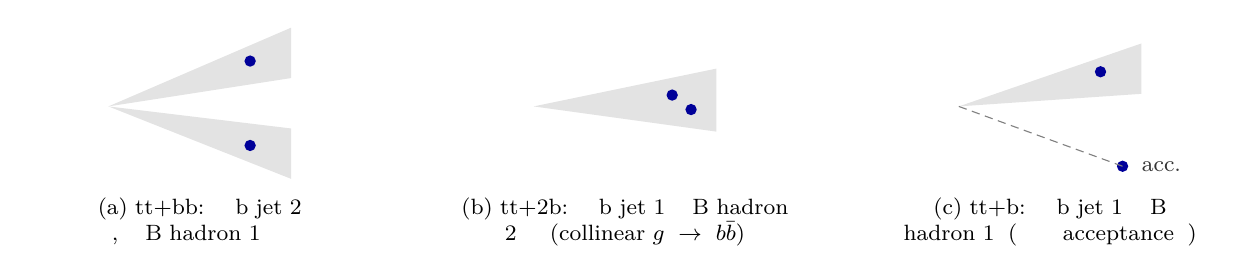
\begin{tikzpicture}[x=0.8cm, y=0.8cm, font=\footnotesize,
  lab/.style={align=center, text width=4.3cm, inner sep=1pt, anchor=north}]
\begin{scope}
  \fill[gray!22] (0,0) -- (2.9,1.25) -- (2.9,0.45) -- cycle;
  \fill[gray!22] (0,0) -- (2.9,-0.35) -- (2.9,-1.15) -- cycle;
  \fill[blue!60!black] (2.25,0.72) circle (0.09);
  \fill[blue!60!black] (2.25,-0.62) circle (0.09);
  \node[lab] at (1.45,-1.4) {(a) tt+bb: 추가 b jet 2 개, 각각 B hadron 1 개 이상};
\end{scope}
\begin{scope}[xshift=5.4cm]
  \fill[gray!22] (0,0) -- (2.9,0.6) -- (2.9,-0.4) -- cycle;
  \fill[blue!60!black] (2.2,0.18) circle (0.09);
  \fill[blue!60!black] (2.5,-0.05) circle (0.09);
  \node[lab] at (1.45,-1.4) {(b) tt+2b: 추가 b jet 1 개에 B hadron 2 개 이상(collinear $g\to b\bar b$)};
\end{scope}
\begin{scope}[xshift=10.8cm]
  \fill[gray!22] (0,0) -- (2.9,1.0) -- (2.9,0.2) -- cycle;
  \fill[blue!60!black] (2.25,0.55) circle (0.09);
  \fill[blue!60!black] (2.6,-0.95) circle (0.09);
  \draw[densely dashed, gray] (0,0) -- (2.6,-0.95);
  \node[anchor=west, gray!40!black] at (2.75,-0.95) {acc.\ 밖};
  \node[lab] at (1.45,-1.4) {(c) tt+b: 추가 b jet 1 개에 B hadron 1 개(다른 하나는 acceptance 밖)};
\end{scope}
\end{tikzpicture}
\caption{GenHFHadronMatcher 에 의한 추가 b jet 범주(AN 의 Fig.~5 를 따라 다시 그림). 회색 원뿔은 생성자 수준 jet, 점은 B hadron.}
\label{fig:samples-hfmatch}
\end{figure}

\begin{itemize}
  \item \textbf{SL}: tt+cc·tt+LF 는 5FS \ttbar, tt+b·tt+2b·tt+bb 는 4FS \ttbb 에서 가져와 DNN 노드 tt+mb 로 묶는다\src{AN-22-122 v26, PDF p.14, l.341--346}. tt+bbb·tt+4b 는
        노드 tt+nb 로 묶고, 4FS 의 통계가 모자라 "절충안으로" LO tt4b 에서 가져온다\src{AN-22-122 v26, PDF p.15, l.349--360}. 부록 D 의 표본별 사용 범주도
        같다\src{AN-22-122 v26, PDF p.187, p.195, p.203}. 최종 fit 은 "5j4b model option 2" 다.
  \item \textbf{DL}: \ttbar 와 tt+4b 를 한 노드로 다루고, "생성자 수준에서 b-tag jet 넷인 사건을 \ttbar 표본에서 제외"한 뒤 tt+4b 를 더한다
        \src{AN-22-122 v26, PDF p.17, l.372--376}. 정확히 어느 범주를 뺐는지는 확인 못 함.
  \item \textbf{승인(SL 최종)}: tt+mb $=$ tt+$\leq$2b, tt+nb $=$ tt+$\geq$3b\src{승인 발표 p.18}. fit 은 \ttbar(tt+lf, tt+cc)와 $t\bar tb$(tt+nb, tt+mb) 두 template 이고
        ttH·\ttbar·$t\bar tb$ 정규화가 자유다\src{승인 발표 p.25, p.27}.
\end{itemize}
LO tt4b 와 4FS \ttbb 는 tt+nb 에서 jet 수 10 이하는 일치하고 jet 수 $>10$, medium b-tag $>7$ 에서 어긋나지만 그곳에는 신호가 적다
\src{AN-22-122 v26, PDF p.15, l.364--371}. AN 은 tt+4b 를 4FS 에서 NLO 로 얻으려고 약 6 배 큰 4FS 표본을 요청했고 Run~3 에서 추진한다
\src{AN-22-122 v26, PDF p.14, l.329--338}.

\begin{andiff}[AN 서술의 혼선 — "Option 1/2"]
본문은 "LO tt4b 로 tt+bbb·tt+4b 를 만드는 것"을 Option~1, "4FS \ttbb 로"를 Option~2 라 부르지만\src{AN-22-122 v26, PDF p.15, l.355--358}, Fig.~7·8 의 캡션과 최종 fit 의
"option 2" 는 반대 정의와 맞는다\src{AN-22-122 v26, PDF p.16, Figs.~7--8}. 부록 D 와 일관된 "tt+nb ← LO tt4b" 를 이름 대신 적는다.
\end{andiff}

\subsection{genTtbarId 해독과 우리 범주}\label{sec:samples-genttbarid}

NanoAOD 의 \code{genTtbarId} 는 GenTtbarCategorizer 가 사건마다 쓰는 정수이고, 우리는 끝 두 자리(\texttt{\%100})만 쓴다\src{ttbarCategorization\_KR §2.2}. 추가 b jet
이 둘 이상이면 53--55 에서 포화되어 3 개와 4 개를 구분하지 못한다(53--55 의 차이는 앞 두 b jet 안의 B hadron 수일 뿐이다)\src{ttbarCategorization\_KR §2.3}. 그래서
MiniAODv2 에서 같은 매칭을 다시 돌려 추가 b jet 이 셋 이상인 사건만 담은 표본별 조회표 \file{ttnb_<sample>.root}(tree \code{TtNb}, 키 (run, lumi, event))를 만들고,
analyzer 가 그 사건의 끝 두 자리를 61/62(정확히 3 개), 71/72(4 개 이상)로 덮어쓴다(확장 ID)\src{ttbarCategorization\_KR §9}\src{ExpandedTtbarId.h}. 조회표의
\code{genTtbarId} 가 NanoAOD 값과 다르면 잘못 짝지은 파일이므로 멈춘다\src{ExpandedTtbarId.h}. 표~\ref{tab:samples-cats} 가 범주의 대응이다.

\begin{table}[htbp]
\centering
\caption{\ttbar+jets 범주의 대응: AN 이름, \texttt{genTtbarId\%100}(확장 ID 포함), 우리 코드의 세 가지 묶음.}
\label{tab:samples-cats}
\footnotesize
\begin{tabularx}{\textwidth}{l L c l l l}
\toprule
AN 범주 & 정의(추가 jet) & \texttt{\%100} & \texttt{TtCat}(검증용) & stitch 라벨 & b-tag 정규화 group \\
\midrule
tt+LF  & 추가 b·c jet 없음 & 0 & \texttt{LightFlavour} & \texttt{LF} & tt+LF \\
tt+cc  & 추가 c jet $\geq1$, b 없음 & 41--45 & \texttt{AddCjet} & \texttt{cc} & tt+cc \\
tt+b   & 추가 b jet 1 개(B hadron 1 개) & 51 & \texttt{Add1Bjet\_1Had} & \texttt{ttb} & tt+B \\
tt+2b  & 추가 b jet 1 개(B hadron $\geq2$) & 52 & \texttt{Add1Bjet\_2Had} & \texttt{ttb} & tt+B \\
tt+bb  & 추가 b jet 2 개 & 53--55 & \texttt{Add2Bjet} & \texttt{tt2b} & tt+B \\
tt+bbb & AN: $\geq3$(4 제외); 확장 ID: 정확히 3 & 61, 62 & (\texttt{Add2Bjet}) & \texttt{ttbbb} & tt+nb \\
tt+4b  & AN: 정확히 4; 확장 ID: $\geq4$ & 71, 72 & (\texttt{Add2Bjet}) & \texttt{tt4b} & tt+nb \\
\bottomrule
\end{tabularx}
\par\smallskip\footnotesize 출처: AN-22-122 v26, PDF p.12--13; ttbarCategorization\_KR §2.2, §9.2; compute\_stitch\_factors.py \texttt{CAT\_OF\_SUB}; Config\_TtCatGroup.hh \texttt{Classify}.
b-tag 정규화 group 은 이 밖에 ttH, ttHH, ttZH4b, ttZZ4b 가 있어 모두 8 개다\src{STATUS, Known constraints}.
\end{table}

\begin{note}[이름의 함정: "tt2b"]
stitching 라벨 \texttt{tt2b} 는 53--55, 곧 \emph{추가 b jet 이 둘}인 사건(AN 의 tt+bb)이고 AN 의 "tt+2b" 는 52 다. \file{compute_stitch_factors.py} 의 출력 머리글도
"tt+2b(53-55)" 다. \code{TtCat} 이름(\code{Add1Bjet_2Had} 등)은 이 혼동을 피하려고 붙였다\src{ttbarCategorization\_KR §3.2}. 확장 ID 의 경계(정확히 3 / $\geq4$)는
AN(3 이상·4 제외 / 정확히 4)과 다르지만 둘 다 tt+nb 로 합치므로 결과는 같다(우리 판단).
\end{note}

STEP~17 이후 공식 범주(\code{officialTtCategory()})는 NanoAOD \code{genTtbarId} 의 해독이고, analyzer 의 GenPart 알고리즘과의 2-way 비교를 검증 히스토그램으로 남긴다
\src{STEP 17}. 예전 메모의 "tt+b 부터 tt+4b 까지 tt+nb 노드 하나로"\src{ttbarCategorization\_KR §3.3}는 AN 의 두 노드(tt+mb, tt+nb) 구조와 다르며, AN 쪽이 맞다.

% -----------------------------------------------------------------------------
\section{Stitching: 5FS \texorpdfstring{\ttbar}{ttbar}, 4FS \texorpdfstring{\ttbb}{ttbb}, LO tt4b}\label{sec:samples-stitch}

\subsection{왜 필요한가와 선례}

5FS 포괄 \ttbar 에도 tt+bb, tt+nb 사건이 적은 통계로 들어 있으므로 세 표본을 그냥 더하면 그 위상공간이 두세 번 세어진다. stitching 은 각 범주를 한 표본
(dedicated)에만 맡기고 그 표본을 다시 정규화해, 4FS 의 모델링과 통계를 이중 계산 없이 쓰게 한다\src{ttbarCategorization\_KR §10.1}. ttH(bb) 의 처방은 명시적이다:
tt+B($=$ tt+bb, tt+b, tt+2b)는 4FS 에서, tt+C·tt+LF 는 5FS 에서 가져오고, 바꿔 넣은 tt+B 의 수율이 포괄 표본에서 \emph{대체된} tt+B 부분의 수율과 같도록 weight 를
준다 — 그래서 \ttbar 전체 수율은 그대로이고 tt+B 정규화는 fit 에서 자유다\src{AN-19-094 v20, PDF p.89, §6.2.1}. 우리 발표의 표도 같은 구조이고(5FS: lf·cc 만 ×1;
\ttbb: b, 2b, bb 를 ×$r$; tt4b: bbb, 4b 를 ×$r$), 같은 stitching 을 analyzer 와 b-tag SF 정규화에 똑같이 써야 수율이 닫힌다\src{Hbb 회의 FH 발표 p.21}\src{STATUS, Known constraints}.

\subsection{우리 공식과 기호}\label{sec:samples-stitch-formula}

\file{compute_stitch_factors.py} 의 기본 계획 \code{EXP} 를 적는다\src{compute\_stitch\_factors.py, STITCH\_PLANS, CAT\_OF\_SUB}. 기호: $c\in\{\mathrm{Had},\mathrm{SL},\mathrm{DL}\}$
는 \ttbar 의 W 붕괴 채널($\mathrm{BR}_{\mathrm{Had}}=0.45441081$, $\mathrm{BR}_{\mathrm{SL}}=0.43937838$, $\mathrm{BR}_{\mathrm{DL}}=0.10621081$), $\sigma_{\mathrm{tot}}=831\,760\fb$ 는
포괄 \ttbar 단면적(DB), $G_s(S)=\sum_{i\in s,\ \mathrm{ID}_i\%100\in S}g_i$ 는 표본 $s$ 에서 확장 ID 가 집합 $S$ 에 드는 사건의 genWeight 합(prescan; $G_s\equiv G_s(\mathrm{all})$),
$\sigma_{\mathrm{ded}}$ 는 dedicated 표본의 DB 유효 단면적 $\sigma\times\mathrm{BR}$ 이다(4FS: $\sigma_{\ttbb,c}=1452\fb\times\mathrm{BR}_c$; tt4b: $\sigma_{\mathrm{tt4b}}=296\fb$, 붕괴
inclusive). 채널마다의 4FS \ttbb 는 자기 채널의 포괄 표본 \file{TTbar_c} 에 묶이고(anchor) 53--55 를 맡으며, tt4b 는 세 포괄 표본을 합친 것에 묶이고 61, 62, 71, 72 를
맡는다:
\begin{align}
  f_{B,c} &= \frac{G_{\mathrm{TTbar}_c}(53,54,55)}{G_{\mathrm{TTbar}_c}}, &
  r_{B,c} &= \frac{\sigma_{\mathrm{tot}}\,\mathrm{BR}_c\,f_{B,c}}{\sigma_{\ttbb,c}}, \label{eq:samples-rB}\\
  f_{4b}  &= \frac{\sum_c G_{\mathrm{TTbar}_c}(61,62,71,72)}{\sum_c G_{\mathrm{TTbar}_c}}, &
  r_{4b}  &= \frac{\sigma_{\mathrm{tot}}\,f_{4b}}{\sigma_{\mathrm{tt4b}}}. \label{eq:samples-r4b}
\end{align}
사건마다 곱하는 배수 $m_{\mathrm{stitch}}(s,c_i)$ 는 포괄 표본에서 맡기지 않은 범주(LF, cc, 51--52)는 1, 넘긴 범주(53--55, 61--72)는 0; dedicated 표본에서 맡은 범주는
$r$, 나머지는 0; 계획 밖의 표본은 1 이다\src{compute\_stitch\_factors.py, build\_analyzer\_table}. dedicated 사건 하나의 weight 는 식~\eqref{eq:samples-weight} 와 곱하면
\begin{equation}
  w_i = \frac{L\,\sigma_{\mathrm{ded}}}{G_{\mathrm{ded}}}\,g_i\cdot r = \frac{L\,\sigma_{\mathrm{inc}}\,f}{G_{\mathrm{ded}}}\,g_i,
  \qquad \sigma_{\mathrm{inc}}=\sigma_{\mathrm{tot}}\mathrm{BR}_c\ (\text{또는 }\sigma_{\mathrm{tot}})
  \label{eq:samples-dedw}
\end{equation}
이 되어 $\sigma_{\mathrm{ded}}$ 가 약분된다. 그래서 4FS 단면적 1452\fb 의 정확한 의미(STEP~10 이 지적한, ttH AN 이 쓴 LHE 총 단면적 43.74\pb 와의 30 배 차이
\src{STEP 10}\src{AN-19-094 v20, PDF p.90, l.956--963})는 결과에 들어가지 않는다. 필요한 것은 base weight 와 $r$ 이 \emph{같은} $\sigma_{\mathrm{ded}}$ 를 쓰는 것뿐이고,
단일 DB 가 그것을 보장한다\src{STEP 11}. 표~\ref{tab:samples-owner} 는 범주별 담당 표본을 AN, ttH(bb), 우리 Run~2 계획, 지금의 2024 로 나란히 놓은 것이다.

\begin{table}[htbp]
\centering
\caption{범주별 담당 표본(stitching). 5FS = 포괄 \ttbar, 4FS = \ttbb, tt4b = LO tt4b.}
\label{tab:samples-owner}
\footnotesize
\begin{tabularx}{\textwidth}{l c C C C C}
\toprule
범주 & \texttt{\%100} & AN SL (부록 D) & ttH(bb) & 우리 Run~2 (\texttt{EXP}) & 우리 2024 (지금) \\
\midrule
tt+LF  & 0      & 5FS & 5FS & 5FS ($\times1$) & 5FS \\
tt+cc  & 41--45 & 5FS & 5FS & 5FS ($\times1$) & 5FS \\
tt+b   & 51     & 4FS & 4FS & \textbf{5FS} ($\times1$) & 5FS \\
tt+2b  & 52     & 4FS & 4FS & \textbf{5FS} ($\times1$) & 5FS \\
tt+bb  & 53--55 & 4FS & 4FS & 4FS ($\times r_{B,c}$) & 5FS \\
tt+bbb & 61, 62 & tt4b & 4FS(tt+B 안) & tt4b ($\times r_{4b}$) & 5FS(53--55 안) \\
tt+4b  & 71, 72 & tt4b & 4FS(tt+B 안) & tt4b ($\times r_{4b}$) & 5FS(53--55 안) \\
\bottomrule
\end{tabularx}
\par\smallskip\footnotesize 출처: AN-22-122 v26, PDF p.187, 195, 203; AN-19-094 v20, PDF p.89; compute\_stitch\_factors.py; D-2026-10-05-C.
\end{table}

\begin{andiff}[우리 \texttt{EXP} 가 AN 과 다른 점: 추가 b jet 하나(51, 52)]
AN(부록 D), ttH(bb), 그리고 우리 Hbb 발표의 표는 모두 tt+b(51)와 tt+2b(52)를 4FS \ttbb 에서 가져온다. 지금 \code{EXP} 는 이 둘(라벨 \texttt{ttb})을 5FS 포괄 표본에
남기고 4FS 에는 53--55 만 맡긴다\src{compute\_stitch\_factors.py, l.245--283, l.325--333}. 옛 선택지 \code{A}·\code{B} 는 포괄에 LF+cc 만 남겼으므로\src{compute\_stitch\_factors.py, l.98--99}
어느 시점에 바뀐 것인데 그 근거를 적은 기록은 찾지 못했다. 2017 \file{TTToHadronic} 에서 51+52 의 genWeight 비율(2.0\,\%)은 53--55(0.42\,\%)의 약 4.8 배라(우리 계산)
\src{ttbarCategorization\_KR §10.7.2} 이 선택은 $n_b\geq3$ 영역의 \ttbar 구성에 직접 영향을 준다. 분석자가 정할 항목이다(\S\ref{sec:samples-openq}).
\end{andiff}

\begin{note}[정규화 조건의 점검 — 이 문서를 쓰며 찾은 의문]
ttH 의 처방은 "맡은 범주에서 dedicated 의 수율 $=$ 포괄 표본이 그 범주에 주던 수율", 곧 $\sum_{i\in\mathrm{ded,owned}}w_i=L\,\sigma_{\mathrm{inc}}f$ 이다.
식~\eqref{eq:samples-dedw} 를 맡은 범주에 대해 더하면
\begin{equation}
  \sum_{i\in\mathrm{ded,owned}} w_i = L\,\sigma_{\mathrm{inc}}\,f\;\frac{G_{\mathrm{ded}}(\mathrm{owned})}{G_{\mathrm{ded}}} \equiv L\,\sigma_{\mathrm{inc}}\,f\;p_{\mathrm{own}}
  \label{eq:samples-pown}
\end{equation}
이므로 조건은 $p_{\mathrm{own}}=1$, 곧 dedicated 표본의 사건이 모두 맡은 범주에 있을 때만 성립한다. 커밋된 2017 prescan(\file{prescan_summary/prescan_summary.json},
tt+nb 조회표 없음)의 genWeight 합으로 계산하면 $p_{\mathrm{own}}$(53--55) 은 \file{TTbb_Hadronic} 0.114, \file{TTbb_SemiLep} 0.108, \file{TTbb_DiLep} 0.103 이다
\src{D-2026-10-10-C}. 4FS \ttbb 의 genWeight 합 가운데 LF(0)가 43--46\,\%, 51--52 가 약 41\,\% 다(우리 계산). 조회표가 있던 2026-06 실행의 합으로는 53--55 가
0.109/0.104/0.100, \file{TT4b} 의 61--72 가 0.198 이다(우리 계산)\src{ttbarCategorization\_KR §10.7.2}; 커밋된 prescan 에는 61--72 가 없어 \file{TT4b} 의 값은 그
실행에서만 나온다. 그렇다면 지금 공식의 stitched tt+bb 는 포괄 예측의 약 1/9, tt+nb 는 약 1/5 이 된다. 처방대로라면 분모를 맡은 범주의 합으로 바꿔
$r'=r/p_{\mathrm{own}}=\sigma_{\mathrm{inc}}f/(\sigma_{\mathrm{ded}}\,p_{\mathrm{own}})$ 이어야 한다(우리 판단, D-2026-10-10-C 로 PROPOSED; 예: Had 에서 $r\approx2.4$ 대신
약 22). STEP~11 의 검증(V4)은 $\sigma_{\mathrm{ded}}$ 의 약분만 보았다\src{STEP 11}.
생성자 수준의 closure — prescan 합으로 $\sum_{\mathrm{TTbb}_c,\,53\text{--}55}w$ 와 $\sum_{\mathrm{TTbar}_c,\,53\text{--}55}w$ 를 비교 — 로 바로 확인할 수 있다.
2017 Hbb 발표에서 $n_b$ 와 함께 Data/MC 가 커진 것이\src{Hbb 회의 FH 발표 p.25--26} 이와 관련 있는지는 그 plot 이 쓴 stitch JSON 을 확인한 뒤 판단한다.
\end{note}

\subsection{지금까지의 값과 상태}\label{sec:samples-stitch-values}

2026-06 의 2017 실행(옛 이름, lumi 41480\pb$^{-1}$, 당시의 $\sigma_{\mathrm{ded}}$ 관례 1.452\pb)은 $f_{B}=0.004187/0.003829/0.003504$(Had/SL/DL),
$r_{B}=1.090/0.9967/0.9121$, $f_{4b}=9.8\times10^{-5}$, $r_{4b}=0.2759$ 를 주었다\src{ttbarCategorization\_KR §10.7.2}. $r_{4b}<1$ 은 tt4b 의 \emph{전체}
단면적(0.296\pb)이 포괄 표본이 61--72 에 주는 예측($\sigma_{\mathrm{tot}}f_{4b}\approx0.082\pb$)의 약 3.6 배라서다. 이 비교는 tt4b 사건 가운데 맡은 범주에 드는
몫($p_{\mathrm{own}}\approx0.2$)을 빠뜨린 것이다(\S\ref{sec:samples-stitch-formula} 의 마지막 상자). 채널마다 $f_B$ 가 달라 Had 의 $r$ 을 SL·DL 에 쓰면 9--20\,\% 어긋나므로 채널별로
stitch 한다\src{STITCH\_CHANGELOG §2}. DB 통일 뒤에는 $r_{B,\mathrm{Had}}\approx2.40$($831\,760\times0.004187/1452$, 우리 계산)이 되고 base weight 도 함께 바뀌어 곱은
같다\src{STEP 11}. 저장소의 \file{DerivedCorr/stitchFactors/stitch_factors_2017.json} 은 KNU 의 로컬 수정이 커밋된 판으로\src{STATUS 2026-10-05} lumi 41480,
$r_B=2.460/2.247/2.053$, $f_{4b}=r_{4b}=0$ 이다. $f_{4b}=0$ 은 그 prescan 이 tt+nb 조회표 없이 돌았기 때문이다: 커밋된 \file{prescan_summary.json} 에는
61--72 가 하나도 없고, 그래서 tt+$\geq$3b 는 53--55 에 남아 4FS 가 맡는다\src{D-2026-10-10-C}. 2017 v20 의 파생 입력(stitch, 조회표)은 아직 다시 만들지 않았고
main·prescan yml 의 경로는 \code{null}(꺼짐)이며, btagtrig yml 만 이 JSON 과 조회표 디렉터리를 읽는다(b-tag 정규화 재가중 유도용)\src{D-2026-06-30-E}\src{STATUS, Current correction state}\src{D-2026-10-10-C}.

\subsection{2024 와 2018}\label{sec:samples-stitch-2024}

2024 에는 tt+nb 조회표가 없다(NtupleForge V6 미착수). 그래서 2024 job 은 조회표 없이 돌아(\code{EraConfig::hasTtNbLookup("2024")} 가 거짓) 61--72 가 나오지 않고
tt+$\geq$3b 는 tt+B(51--55) 안에 남으며, stitching 도 하지 않는다(\code{path_stitch_json: null}). 4FS \file{TTbb_*} 와 \file{TT4b} 는 돌리지만 포괄 \ttbar 위에 쌓지
않으므로 지금은 5FS 포괄 하나가 모든 범주를 낸다\src{D-2026-10-05-C}\src{D-2026-10-02-A}. 2024 에 stitching 을 켜기 전에 둘을 정리한다: (1) skim 된 \code{Events} 로
prescan 하면 $f$·$r$ 이 skim 뒤의 합으로 조용히 틀리므로(합성 시험에서 $f$(53--55) $\times1.61$)\src{PLAN\_v15 §2 \#8} NtupleForge 의 job 별 \code{ForgeAudit}(skim 전
\texttt{genTtbarId\%100} 별 Σw)를 쓴다\src{PLAN\_v15 §9.4}; (2) 위의 $p_{\mathrm{own}}$ 문제. 2018 은 조회표가 여섯 표본에 있지만 v15 에 \file{TT4b} 가 없어, \code{EXP}
가 \file{TT4b} 를 가정하면 tt+nb 가 조용히 빠진다\src{PLAN\_v15 §2 \#7}\src{PLAN\_v15 §9.4}.

\begin{impl}
\begin{itemize}
  \item 계산: \file{compute_stitch_factors.py} — \code{STITCH_PLANS["EXP"]}, \code{CAT_OF_SUB}, \code{compute_plan}, \code{build_analyzer_table}; 출력
        \file{DerivedCorr/stitchFactors/stitch_factors_<연도>.json} 의 \code{analyzer_perEvent_factor}. $\sigma$ 는 env \code{TTHH_XSEC_DB} 또는 \file{data/samples_2017UL.json}.
  \item 적용: \file{src/StitchFactors.cc} 의 \code{factor(expandedId, w)}, 확장 ID 는 \file{include/ExpandedTtbarId.h} 의 \code{resolve(run, lumi, event, genTtbarId)};
        \code{process()} 에서 \code{_evtWeight *= stitchMult} 후 tree 에 \code{stitchWeight}, \code{expandedTtbarId} 를 쓴다. 경로는 yml \code{common.path_stitch_json},
        \code{common.path_expanded_ttbarid_dir}\src{README §4}, 실패 코드는 60--63(stitch), 70--73(확장 ID)\src{ERROR\_CODES}.
\end{itemize}
\end{impl}

% -----------------------------------------------------------------------------
\section{변경 이력}\label{sec:samples-history}

표~\ref{tab:samples-history} 는 이 장의 내용과 관련된 변경 기록을 시간순으로 모은 것이다(자세한 내용은 각 기록).

\begin{table}[htbp]
\centering
\caption{표본·정규화·stitching 의 주요 변경(날짜는 2026 년; STEP 은 \texttt{docs/changes}, D-… 는 DECISIONS 의 기록).}
\label{tab:samples-history}
\footnotesize
\begin{tabularx}{\textwidth}{>{\raggedright\arraybackslash}p{1.25cm} >{\raggedright\arraybackslash}p{2.75cm} L}
\toprule
날짜 & 기록 & 내용 \\
\midrule
06 & STEP~1, STITCH\_\allowbreak CHANGELOG & \code{stitchWeight} branch; 채널별 4FS stitch(\code{EXP}), 확장 ID 61--72, 사건별 적용 \\
06-12/14 & STEP~10, 11 & 4FS 단면적의 의미 의문(1.452\pb 대 LHE 43.74\pb); 단면적 DB 단일 출처(\ttbb SL·DL 2.2 배 과소 해소) \\
06-15 & STEP~12, 14 & fb 단위, AN 기준 $\sigma$·BR, k-factor 미적용; 세 weight tier \\
06-29/30 & STEP~17; D-06-30-A, B, E & 2017 \file{fullNano_v20}, \code{genTtbarId} 해독; 표본 이름 = NtupleForge key; v20 파생 보정 \code{null} \\
07-26/29 & CHANGELOG & 2018 DB(85 표본), 2018 lumi 59.83 → 59.56; stitch·조회표 이름 별칭과 FATAL \\
10-02 & D-10-02-A, D, E & 2024 먼저; 2017 lumi 42.07; blinding 정책 \\
10-05 & D-10-05-A, C, D & 2024 첫 look(109.816\fbinv, 임시 $\sigma$), tt+nb 조회표·stitching 없이; 2017 v20 삭제 \\
10-06/07 & D-10-06-A; D-10-07-A, B & ParkingHH 와 PD 규칙; 2024 main 다시; W·DY 표본은 저장 공간을 본 뒤 \\
\bottomrule
\end{tabularx}
\end{table}

% -----------------------------------------------------------------------------
\section{미결 사항}\label{sec:samples-openq}

\begin{openq}[2 장의 미결 사항(분석자 결정 또는 확인)]
\begin{enumerate}
  \item \textbf{stitching 의 정규화 조건}(\S\ref{sec:samples-stitch-formula} 의 마지막 상자): dedicated 수율이 포괄 예측의 $p_{\mathrm{own}}$ 배(\ttbb 약 0.11, tt4b 약 0.2)인지
        생성자 수준 closure 로 확인하고, 맞으면 $r$ 을 맡은 범주의 합으로 정규화한다(D-2026-10-10-C, PROPOSED). b-tag 정규화 재가중과 그 JSON 도 같은 stitching 으로 다시 만든다.
  \item \textbf{51·52 의 담당}: AN·ttH·우리 발표처럼 4FS 로 옮길지, 지금처럼 5FS 에 둘지(근거 기록 없음; D-2026-10-10-C (b), AI 권고는 AN 대로).
  \item 2016 의 PD(BTagCSV 사용 여부)·루미노시티·표본 DB; 2018 brilcalc; 2024 루미노시티 불확도와 연도 간 상관; SL·DL 과 맞출 lumi 값(AN 41.53/59.74 대 우리 값).
  \item 단면적: 2024 의 모든 $\sigma$(임시; 특히 비율로 올린 6 항목), Run~2 DB 의 \code{verify_xsec} 항목, \ttZ 861 대 841\fb(AN 내부 불일치; DB 는 분석자 결정으로 861
        \src{samples\_2017UL.json, TTZToBB}), 다중 top·ttVV 의 출처 표기, \file{ST_s_had} 의 note("sigma remains undetermined" 인데 값이 있음).
  \item 표본: Run~2 v15 의 부재 5 종, 2024 W$\to\ell\nu$·DY 생산, 2024 tt+nb 조회표(V6)와 skim 전 범주 합으로 하는 2024 stitching. 데이터: 빠진 golden LS 를 되살릴지,
        세 PD 공통 LS mask 와 그 brilcalc 로 갈지.
\end{enumerate}
\end{openq}

% =============================================================================
% 3 장 트리거와 트리거 SF  (AN_KR v0.1, 2026-10-10)
% 출처: AN-22-122 v26 §4.3, AN-19-094 v20 §3.1, Hbb 회의 FH 발표, KCMS 발표,
%       tempTTHH STEP 14·16·24·26, DECISIONS(D-2026-06-30-E, D-2026-10-05-A·B, D-2026-10-06-A, D-2026-10-07-A),
%       PLAN_v15 §9, ROADMAP_FH §3·§6, LUMI_SOURCES §6, 코드(EraConfig.h, SelectionCuts.h,
%       ttHHanalyzer_unified.cc, src/CorrectionsManager.cc, TriggerStudy/)
% =============================================================================
\chapter{트리거와 트리거 SF}\label{ch:trigger}

FH 사건에는 lepton 이 없으므로 다중 jet, 큰 \HT, 온라인 b-tag 을 요구하는 강입자(hadronic) trigger 경로들의
OR 로 사건을 모은다. 오프라인 문턱(\HT{} $>500\GeV$, jet 6 개 이상, 여섯째 jet $\pt>40\GeV$)은 ttH(bb) FH 분석을
따르지만 이 OR 의 효율이 평탄해지는 영역(plateau) 위에 완전히 있지는 않다. 그래서 단일 muon trigger 를 기준(reference)으로
data 와 MC 의 trigger 효율을 재고, 그 비인 scale factor(SF, data/MC 효율 비)를 \HT{} $\times$ 여섯째 jet \pt{} $\times$ b-tag
수의 함수로 MC 에 곱한다. 2017 은 이 SF 를 유도해 적용했다. 2024 는 경로가 ParticleNet(PNet) 판으로 바뀌었고 b-tag 경로가
\texttt{ParkingHH} PD 에만 기록된다는 것이 확인되어 PD 규칙을 새로 정했으며, SF 유도 도구는 연도를 지원하도록 고쳤지만 2024 SF
자체는 아직 없다(2026-10-10). Run 2 ttHH AN(SL·DL)은 lepton trigger 를 쓰므로, 이 장의 방법은 대부분 ttH(bb) FH AN 에서 온다.

% -----------------------------------------------------------------------------
\section{물리적 배경: 강입자 trigger, turn-on, SF}\label{sec:trigger-theory}

\paragraph{왜 다중 jet + \HT{} + 온라인 b-tag 인가.}
QCD multijet 의 단면적은 신호보다 일곱–여덟 자릿수 크다(예: 2017 표본 \texttt{QCD\_HT500to700} 의 $3.02\times10^{7}\fb$\src{Hbb 회의 FH 발표 p.49} 대 $\sigma(\ttHH)=0.756\fb$\src{AN-22-122 v26, PDF p.23, Table 9}). jet 수와 \HT{} 만으로 rate 를 감당하려면 문턱을 아주 높여야 하고
(예: \code{HLT_PFHT1050} 은 온라인 \HT{} 1050\GeV), 그러면 FH ttHH 의 대부분이 빠진다. 온라인 b-tag 을 1–3 개 요구하면
QCD 의 rate 가 크게 줄어 운동학 문턱을 낮출 수 있다. ttH(bb) FH 를 위해 만든 경로들이 바로 이 구조다: jet 6 개와 b-tag 1 개
(6J1T), jet 6 개와 b-tag 2 개(6J2T), 그리고 b-tag 을 3 개로 늘리는 대신 jet 문턱을 낮춘 jet 4 개 경로(4J3T)이며, 여기에 b-tag
없는 \code{HLT_PFHT1050} 을 OR 로 더한다\src{AN-19-094 v20, PDF p.32, p.34, p.36}.

\paragraph{효율과 turn-on.}
trigger 의 효율은 오프라인 변수 $x$(여기서는 \HT, 여섯째 jet 의 \pt, b-tag 수)의 함수로 정의한다:
\begin{equation}
  \varepsilon(x) \;=\; \frac{N(\text{offline} \wedge \text{ref} \wedge \text{target} \,|\, x)}
                              {N(\text{offline} \wedge \text{ref} \,|\, x)} .
  \label{eq:trigger-eff}
\end{equation}
분모는 오프라인 선택과 기준 trigger 를 통과한 사건, 분자는 그중 측정 대상(target) trigger 도 통과한 사건이다(ttHH AN 의 식 2 와
같은 정의\src{AN-22-122 v26, PDF p.23, Eq. 2}). 온라인 \HT{} 와 jet \pt{} 는 HLT 의 PF jet 과 온라인 보정으로 계산되므로
오프라인 값과 사건마다 다르다. 그래서 온라인 문턱 하나가 오프라인 변수에서는 계단이 아니라 완만하게 오르는 곡선(turn-on)이 되고,
충분히 높은 곳에서 평탄해진다(plateau). 온라인 b-tag 판별자(2017 CSVv2, 2018 DeepCSV, 2024 PNet)와 오프라인 판별자(DeepJet,
UParTAK4)가 다르면 b-tag 다리(leg)의 turn-on 도 오프라인 b-tag 수의 함수로 번진다\src{AN-19-094 v20, PDF p.33}.
그림~\ref{fig:trigger-turnon} 은 이 구조를 개념적으로 보인다.

\begin{figure}[htbp]
\centering
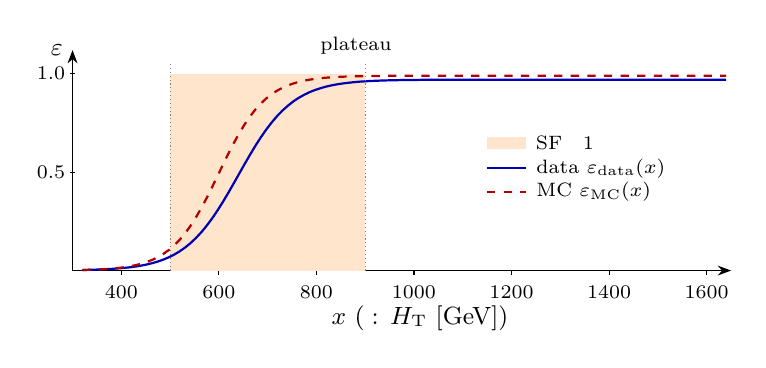
\begin{tikzpicture}[x=0.0062cm,y=2.5cm,>=Stealth]
  % 축
  \draw[->] (300,0) -- (1650,0);
  \node[font=\small] at (975,-0.24) {오프라인 $x$ (예: \HT{} [GeV])};
  \draw[->] (300,0) -- (300,1.12) node[left,font=\small] {$\varepsilon$};
  \foreach \v in {0.5,1.0} \draw (295,\v) -- (305,\v) node[left,font=\scriptsize] {\v};
  \foreach \t in {400,600,800,1000,1200,1400,1600} \draw (\t,0) -- (\t,-0.025) node[below,font=\scriptsize] {\t};
  % turn-on: data 와 MC (logistic, 개념도)
  \fill[orange!20] (500,0) rectangle (900,1.0);
  \draw[thick,blue!70!black,domain=320:1640,samples=120] plot (\x,{0.97/(1+exp(-(\x-640)/55))});
  \draw[thick,red!70!black,dashed,domain=320:1640,samples=120] plot (\x,{0.99/(1+exp(-(\x-600)/48))});
  % 오프라인 문턱과 plateau
  \draw[gray,densely dotted] (500,0) -- (500,1.05) node[above,font=\scriptsize,black] {오프라인 문턱};
  \draw[gray,densely dotted] (900,0) -- (900,1.05) node[above,font=\scriptsize,black] {plateau 시작};
  % 범례
  \fill[orange!20] (1150,0.62) rectangle (1230,0.68); \node[right,font=\scriptsize] at (1230,0.65) {SF 가 1 에서 벗어나기 쉬운 곳};
  \draw[thick,blue!70!black] (1150,0.52) -- (1230,0.52) node[right,font=\scriptsize,black] {data $\varepsilon_\text{data}(x)$};
  \draw[thick,red!70!black,dashed] (1150,0.40) -- (1230,0.40) node[right,font=\scriptsize,black] {MC $\varepsilon_\text{MC}(x)$};
\end{tikzpicture}
\caption{trigger turn-on 의 개념도(수치는 예시이며 측정값이 아니다). 오프라인 문턱이 plateau 보다 낮으면 data 와 MC 의 turn-on
위치·폭 차이가 그대로 수율 차이가 되므로 SF 가 필요하다.}
\label{fig:trigger-turnon}
\end{figure}

\paragraph{SF 와 그 적용.}
MC 의 trigger 모사(emulation)는 온라인 보정, 온라인 b-tag 의 성능, L1 seed 등을 완벽히 재현하지 못한다. 그래서
\begin{equation}
  \mathrm{SF}(x) = \frac{\varepsilon_\text{data}(x)}{\varepsilon_\text{MC}(x)}, \qquad
  w_\text{MC} \;\to\; w_\text{MC}\cdot \mathrm{SF}(x)\quad(\text{trigger 를 통과한 MC 사건에만})
  \label{eq:trigger-sf}
\end{equation}
로 고친다. SF 는 효율의 보정이므로 trigger 를 통과한 사건(효율의 분자)에만 곱한다. 분모와 분자에 같이 곱하면 효율은 그대로이고,
분모에만 곱하면 반대로 고친다\src{TriggerStudy/docs/ARCHITECTURE.md §5}. 신호 영역에서는 trigger 를 요구하므로 신호 영역의
모든 MC 사건에 곱하는 것과 같다.

\begin{note}[기준 trigger 방법이 성립하는 조건]
식~\eqref{eq:trigger-eff} 의 효율이 신호 영역의 효율과 같으려면, $x$ 가 주어졌을 때 기준 trigger 의 통과 여부가 측정 대상
trigger 의 통과 여부와 상관이 없어야 한다: $P(\text{target}\,|\,\text{ref}, \text{offline}, x) = P(\text{target}\,|\,\text{offline}, x)$.
단일 muon trigger 는 muon 하나로 결정되고 강입자 trigger 는 jet 으로 결정되므로 이 가정이 잘 맞는다. ttH(bb) FH 는 두 trigger 의
상관을 1\,\% 미만으로 추정했다\src{AN-19-094 v20, PDF p.32}. 다른 가정은 SF 가 $x$ 에만 의존한다는 것이다. 측정 표본은
$\ttbar\to\mu+$jets 가 많은 영역이고 적용 표본은 jet 이 더 많고 b 가 더 많은 FH 신호 영역이므로, 둘의 차이가 $x$ 로 대부분
설명되어야 한다. ttH 는 pileup 의존이 \HT{} 에 흡수되고 여섯째 jet \pt{} 와 b-tag 수가 주된 효과를 덮는다고 논증했다
\src{AN-19-094 v20, PDF p.33}.
\end{note}

% -----------------------------------------------------------------------------
\section{Run 2 ttHH AN(SL·DL)에서는}\label{sec:trigger-an}

SL 은 연도별 단일 전자·단일 muon trigger(예: 2017 \code{HLT_Ele32_WPTight_Gsf_L1DoubleEG}, \code{HLT_IsoMu27})를 쓴다
\src{AN-22-122 v26, PDF p.31, Tables 19--21}.
muon 의 SF 는 MUO POG 의 것, 전자의 SF 는 ttH(SL) 분석이 전자 \pt{} 와 supercluster $\eta$ 의 함수로 유도한 것을 그대로 쓰고,
ttHH 위상공간(jet 5 개 이상)에서 2018 \ttbar{} DL MC 와 SingleMuon data 로(기준 \code{HLT_IsoMu24}) 통계 오차 안에서 같음을
확인했다\src{AN-22-122 v26, PDF p.22--25}. DL 은 dilepton 과 단일 lepton trigger 를 stream 별로 OR 하고, ttH 가 MET 기준
trigger 로 잰 SF 를 가져오며, ttH 가 쓴 pre-legacy 표본과 UL 표본의 효율 차이로 1\,\% 계통을 더했다\src{AN-22-122 v26, PDF p.26--28}.
trigger 계통은 shape 이고 연도 간 비상관이다\src{AN-22-122 v26, PDF p.120}.

\begin{andiff}[ttHH AN(SL·DL)과 FH 의 차이]
SL·DL 은 POG 나 ttH 의 lepton trigger SF 를 재사용할 수 있지만, FH 는 강입자 trigger 의 SF 를 직접 재야 한다. ttHH AN 에는 FH 의
trigger 에 관한 내용이 없다(FH 는 ``another Analysis Note, in progress'' 라고만 쓴다\src{AN-22-122 v26, PDF p.5}). 그래서 이 장의
방법은 ttH(bb) FH AN 을 선례로 삼는다\tagours.
\end{andiff}

% -----------------------------------------------------------------------------
\section{참고: ttH(bb) FH AN 에서는}\label{sec:trigger-tth}

\begin{table}[htbp]
\caption{ttH(bb) FH 의 연도별 강입자 trigger 경로(OR)와 PD. 이름의 b-tag 숫자는 온라인 mistag rate 를 뜻한다(2017 Run B 는 판별값
컷)\,\src{AN-19-094 v20, PDF p.32--39, Tables 24--29}.}
\label{tab:trigger-tth-paths}
\centering\small
\begin{tabularx}{\textwidth}{@{}p{2.0cm}L p{2.6cm}@{}}
\toprule
연도·기간 & 경로 & PD \\
\midrule
2016 & \code{HLT_PFHT450_SixJet40_BTagCSV_p056}, \code{HLT_PFHT400_SixJet30_DoubleBTagCSV_p056}, \code{HLT_PFJet450} & JetHT \\
2017 Run B & \code{HLT_PFHT430_SixJet40_BTagCSV_p080}, \code{HLT_PFHT380_SixJet32_DoubleBTagCSV_p075}, \code{HLT_HT300PT30_QuadJet_75_60_45_40_TripeCSV_p07}, \code{HLT_PFHT1050} & JetHT, BTagCSV(4J3T) \\
2017 C--F, MC & \code{HLT_PFHT430_SixPFJet40_PFBTagCSV_1p5}, \code{HLT_PFHT380_SixPFJet32_DoublePFBTagCSV_2p2}, \code{HLT_PFHT300PT30_QuadPFJet_75_60_45_40_TriplePFBTagCSV_3p0}, \code{HLT_PFHT1050} & JetHT, BTagCSV(4J3T) \\
2018 (run $\geq$ 317509), MC & \code{HLT_PFHT450_SixPFJet36_PFBTagDeepCSV_1p59}, \code{HLT_PFHT400_SixPFJet32_DoublePFBTagDeepCSV_2p94}, \code{HLT_PFHT330PT30_QuadPFJet_75_60_45_40_TriplePFBTagDeepCSV_4p5}, \code{HLT_PFHT1050} & JetHT \\
\bottomrule
\end{tabularx}
\end{table}

\begin{itemize}
\item \textbf{경로}: 표~\ref{tab:trigger-tth-paths}. 2016 Run H 에서 L1 \HT{} 가 포화된 jet 을 빠뜨려 높은 \HT{} 의 효율이 떨어진 것을
  \code{HLT_PFJet450} 로 대부분 되찾았다\src{AN-19-094 v20, PDF p.33}. 2017 은 \HT{} turn-on 의 효율 저하 때문에 prescale 없는
  \code{HLT_PFHT1050} 을 더했다\src{AN-19-094 v20, PDF p.36}. 2018 초기 run(315252–317509)은 6J1T·6J2T 의 이름이 다르다
  (Table 29)\src{AN-19-094 v20, PDF p.39}.
\item \textbf{PD 중복 제거(2017)}: 4J3T 가 (어떤 조합으로든) 발화한 사건은 BTagCSV 에서, 나머지 6J1T·6J2T 사건과
  \code{HLT_PFHT1050} 만 발화한 사건은 JetHT 에서 가져온다(Table 27)\src{AN-19-094 v20, PDF p.36}.
\item \textbf{오프라인 문턱}: lepton 0, jet 6 개 이상($\pt>30\GeV$, $|\eta|<2.4$), 여섯째 jet $\pt>40\GeV$(``due to HLT performance''),
  \HT{} $>500\GeV$, DeepJet medium b-tag 2 개 이상, $30<m_{qq}<250\GeV$\src{AN-19-094 v20, PDF p.68, Table 55}.
  2017 오프라인 baseline(원문은 ``pT of sixth jet $<50$ GeV'' 로 적혀 있다)에서 모든 경로가 prescale 없다면 OR 의 효율은 약 82\,\%
  이고, 한 경로의 prescale 때문에 80\,\% 로 줄었다\src{AN-19-094 v20, PDF p.36}.
\item \textbf{효율 측정}: 기준 trigger 는 2016 \code{HLT_IsoMu24}, 2017·2018 \code{HLT_IsoMu27} 이고, 오프라인 muon 이 정확히 하나이며
  lepton veto 를 뺀 FH baseline 을 통과한 사건을 쓴다\src{AN-19-094 v20, PDF p.32}. SF 는 연도별로 \HT{} $\times$ DeepJet medium
  b-tag 수 $\times$ 여섯째 jet \pt{} 의 함수이고, 경로가 run 중에 다시 조정된 2017·2018 은 run 평균 효율로 유도했다. 그림의 bin 은
  b-tag 수 2, 3, $\geq 4$, \HT{} 500/550/600/700/800/1000/1500/2500, 여섯째 jet \pt{} 40/45/50/60/70/120/200\GeV{}(그림 판독)이며,
  사건이 빈 bin 에 들어가면 SF 1 을 쓴다\src{AN-19-094 v20, PDF p.35, Fig. 3}.
\item \textbf{불확도}: bin 별 통계 오차만. 근거는 SF 오차가 통계 지배이고, 기준·대상 trigger 의 상관이 1\,\% 미만이며, pileup 의존은
  \HT{} 로, 주된 효과는 여섯째 jet \pt{} 와 b-tag 수로 덮이고, 2018 의 run 의존이 작다는 것이다\src{AN-19-094 v20, PDF p.32--33}.
  fit 에서는 ``Trigger efficiency'' 가 shape, 연도 간 비상관으로 들어간다\src{AN-19-094 v20, PDF p.147, Table 79}.
\end{itemize}

% -----------------------------------------------------------------------------
\section{우리 FH 분석에서는}\label{sec:trigger-ours}

\subsection{연도별 경로와 PD 규칙}\label{sec:trigger-paths}

경로의 정의와 PD 규칙은 \file{ttHHanalyzer_unified.cc} 의 \code{createObjects} 한 곳에 있고, 결과는 cut-flow 의
\texttt{HadTrigger} 단계와 Tree 의 \code{passHadTrig}·\code{passTrigger_*} 에 남는다. 연도별 상수는 \file{include/EraConfig.h} 가
갖는다(모르는 연도는 FATAL)\tagimpl.

\begin{table}[htbp]
\caption{우리 analyzer 의 강입자 trigger OR 와 Data PD 규칙\,\src{ttHHanalyzer\_unified.cc, createObjects; D-2026-10-06-A}.}
\label{tab:trigger-ours}
\centering\small
\begin{tabularx}{\textwidth}{@{}p{1.25cm}L L@{}}
\toprule
연도 & 경로(6J1T, 6J2T, 4J3T, \HT) & Data PD 규칙 / MC \\
\midrule
2017 & 표~\ref{tab:trigger-tth-paths} 의 2017(era B 는 옛 이름, C--F 와 MC 는 PF 이름) &
BTagCSV: 4J3T; JetHT: (6J1T $\vee$ 6J2T $\vee$ HT) $\wedge\,\neg$4J3T; SingleMuon: OR(SF 측정용); MC: OR \tagimpl \\
2018 & DeepCSV 판(\code{..._PFBTagDeepCSV_1p59}, \code{..._DoublePFBTagDeepCSV_2p94}, \code{..._TriplePFBTagDeepCSV_4p5}), \code{HLT_PFHT1050} &
JetHT 단독 OR(2018 에는 BTagCSV PD 가 없다), SingleMuon: OR; 2018A 초기 run 의 다른 이름은 아직 없음 \tagopen \\
2024 & \code{HLT_PFHT450_SixPFJet36_PNetBTag0p35}, \code{HLT_PFHT400_SixPFJet32_PNet2BTagMean0p50}, 4J3T = \code{..._PNet3BTag_4p3}(Data 는 초기 \code{..._TriplePFBTagDeepJet_4p5} 와 OR), \code{HLT_PFHT1050} &
JetMET0/1: \code{HLT_PFHT1050}; ParkingHH: (4J3T $\vee$ 6J1T $\vee$ 6J2T) $\wedge\,\neg$HT; Muon0/1: OR; MC: OR(4J3T 는 PNet 판만) \tagimpl\tagrunthree \\
2016 & 정의 안 됨(FATAL) & --- \tagopen \\
\bottomrule
\end{tabularx}
\end{table}

2017 의 규칙은 ttH(bb) FH 의 Table 27 과 같다. 2024 의 규칙은 같은 구조에서 두 PD 의 역할을 바꾼 것이다(\S\ref{sec:trigger-run3}).
2018 은 지금 코드가 v9 이름으로만 읽고, 주 구성(run $\geq$ 317509)의 경로 이름만 필수 branch 로 검사하므로 2018A Data 는 멈춘다
\src{ttHHanalyzer\_unified.cc, requireTriggerBranches2018\_; PLAN\_v15 §2 \#9}.

\subsection{오프라인 문턱}\label{sec:trigger-offline}

\file{include/SelectionCuts.h} 의 \code{Cuts::nJets} = 6, \code{Cuts::sixthJetPt} = 40\GeV, \code{Cuts::HT} = 500\GeV{} 는 ttH(bb) FH 의
Table 55 그대로이고, 2017 HLT(\code{SixPFJet40}, \code{PFHT380})의 plateau 를 근거로 한 값이다\src{SelectionCuts.h}\tagimpl.
같은 파일의 머리 주석은 2018(\code{SixPFJet36}, \code{PFHT400}, \code{PFHT330PT30})의 plateau 재확인과, 2018 기준을 \code{HLT_IsoMu24} 로
할 때 lead muon 문턱 29 → 26\GeV{} 를 미결로 적어 둔다\src{SelectionCuts.h; STATUS OPEN 6 P1}. 2024 에서도 \HT{} $>500$ 을 분석 컷으로
둔다: b-tag 경로의 \HT{} 다리(330/400/450\GeV)보다 위이고 ttH(bb) FH 와 같으며, OR 의 turn-on 은 trigger SF 가 맡는다
\src{D-2026-10-06-A (4)}\tagours.

\subsection{trigger SF 의 유도 (\texttt{TriggerStudy/})}\label{sec:trigger-derive}

\begin{figure}[htbp]
\centering
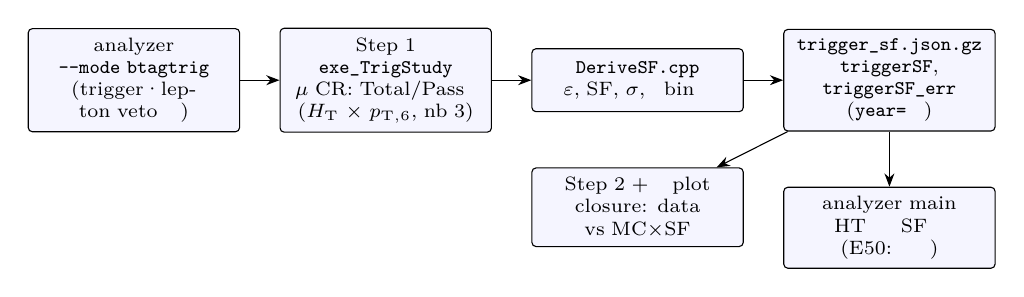
\begin{tikzpicture}[node distance=4mm and 5mm, every node/.style={font=\scriptsize},
  box/.style={draw,rounded corners=1.5pt,align=center,fill=blue!4,minimum height=8mm,text width=2.45cm},
  >=Stealth]
  \node[box] (skim) {analyzer\\ \texttt{--mode btagtrig}\\ (trigger·lepton veto 미적용)};
  \node[box,right=of skim] (s1) {Step 1 \texttt{exe\_TrigStudy}\\ $\mu$ CR: Total/Pass 맵\\ (\HT{} $\times$ $p_{\mathrm{T},6}$, nb 3)};
  \node[box,right=of s1] (der) {\texttt{DeriveSF.cpp}\\ $\varepsilon$, SF, $\sigma$, 빈 bin 채움};
  \node[box,right=of der] (json) {\texttt{trigger\_sf.json.gz}\\ \texttt{triggerSF}, \texttt{triggerSF\_err}\\ (\texttt{year=} 태그)};
  \node[box,below=7mm of json] (ana) {analyzer main\\ HT 단계에서 SF 곱함\\ (E50: 연도 확인)};
  \node[box,below=7mm of der] (s2) {Step 2 + 검증 plot\\ closure: data vs MC$\times$SF};
  \draw[->] (skim) -- (s1); \draw[->] (s1) -- (der); \draw[->] (der) -- (json);
  \draw[->] (json) -- (ana); \draw[->] (json) -- (s2);
\end{tikzpicture}
\caption{trigger SF 의 흐름\,\src{TriggerStudy/README.md; STEP 26}. 같은 btagtrig skim 이 b-tag 효율 맵(\ref{ch:btag} 장)에도 쓰인다.}
\label{fig:trigger-flow}
\end{figure}

\begin{itemize}
\item \textbf{표본}: analyzer 의 \texttt{btagtrig} 모드 skim. 이 모드는 MET filter, PV, jet 6 개 이상, 여섯째 jet $\pt>40$, \HT{} $>500$ 은
  걸지만 강입자 trigger 와 lepton veto 는 걸지 않고 trigger bit 만 기록한다\src{ttHHanalyzer\_unified.cc, kCutSequence}. lead muon
  ($\pt>29\GeV$, tight ID, PF 상대 isolation $<0.15$)이 있는 사건만 lepton 을 모은다(\texttt{requireLeadMuonOnly})\tagimpl.
\item \textbf{측정 영역}: muon 정확히 1 개, 전자 0 개, 기준 trigger 통과. 기준은 2017 \code{HLT_IsoMu27}, 2024 \code{HLT_IsoMu24}
  이고, Data 는 2017 \texttt{SingleMuon\_Run2017B..F}, 2024 \texttt{Muon0/1\_Run2024*} 16 개, MC 는 \texttt{TTbar\_\{DiLep, Hadronic, SemiLep\}}
  이다\src{STEP 26 §1; TriggerStudy/include/Config.hh}. MET 컷은 없다(\code{Config::metCut} = 0): 적용 영역인 FH 에 MET 컷이 없기
  때문이다\src{TriggerStudy/include/Config.hh}\tagours. 사건마다 OR 를 다시 계산해 skim 의 \code{passHadTrig} 와 다르면 멈춘다\src{TriggerStudy/README.md §8}.
\item \textbf{binning}: \HT{} = \{500, 550, 600, 700, 800, 1000, 1500, 2500\}\GeV, 여섯째 jet \pt{} = \{40, 45, 50, 60, 70, 120, 200\}\GeV,
  b-tag 수(오프라인 medium) = \{0--2, 3, $\geq 4$\}, $\eta$ 는 구분하지 않는다(\code{useEta} = false). ttH 의 bin 과 같고, 다만 첫 b-tag 칸이
  0--2 이다(SF 를 b-tag 컷 전, \HT{} 단계에서 곱하기 때문)\src{TriggerStudy/README.md §4-D; Hbb 회의 FH 발표 p.44}\tagimpl.
\item \textbf{효율 오차}: data 는 Clopper--Pearson 68.27\,\% 구간의 반폭, MC(가중 사건)는 유효 사건 수 $N_\text{eff} = (\sum w)^2/\sum w^2$ 로
  $\sigma_\varepsilon = \sqrt{\varepsilon(1-\varepsilon)/N_\text{eff}}$ 이고, SF 의 오차는
  \begin{equation}
    \frac{\sigma_\mathrm{SF}}{\mathrm{SF}} = \sqrt{\Big(\frac{\sigma_{\varepsilon,\text{data}}}{\varepsilon_\text{data}}\Big)^2
    + \Big(\frac{\sigma_{\varepsilon,\text{MC}}}{\varepsilon_\text{MC}}\Big)^2}
    \label{eq:trigger-sferr}
  \end{equation}
  이다\src{TriggerStudy/docs/ARCHITECTURE.md §3; DeriveSF.cpp}. 효율의 오차를 분자(Pass)·분모(Total)의 오차로 독립 전파하는 방식은 같은 사건이
  양쪽에 있어 상관을 무시하므로 쓰지 않았다(data 와 MC 는 서로 독립인 표본이므로 식~\eqref{eq:trigger-sferr} 의 제곱합은 그대로 맞다).
\item \textbf{통계가 적은 bin}: data 통과 $<10$ 사건이거나 MC 통과의 $N_\text{eff}<20$ 이면 한 칸 낮은 \pt{}, 그다음 한 칸 낮은 \HT{} 의
  값으로 채우고(2D log-quadratic fit 은 선택), 상대 오차는 측정 bin 의 중앙값과 5\,\% 중 큰 것 이상, 못 채우면 SF $=1\pm0.5$ 이다
  \src{TriggerStudy/docs/ARCHITECTURE.md §3-B, §3-C}.
\item \textbf{출력}: correctionlib JSON \file{trigger_sf.json.gz} 의 \code{triggerSF}(중앙값)와 \code{triggerSF_err}(오차), 입력
  (\code{nbJets}, \code{eta}, \code{ht}, \code{pt}), \code{nbJets} 경계 [0, 3, 4, 5], (\HT, \pt) multibinning, 범위 밖은 clamp. STEP 26 부터
  description 에 \texttt{year=<YYYY>; reference=...; hadronic OR: ...} 가 들어가고, 측정 bin 이 하나도 없는 범주가 있으면 RESULT FAIL 로
  끝나며 좋은 JSON 을 지우지 않는다\src{STEP 26 §2--3}\tagimpl.
\end{itemize}

\subsection{analyzer 에서의 적용과 weight 의 tier}\label{sec:trigger-apply}

SF 는 \code{applyEventScaleFactors} 에서, 즉 \HT{} $>500$ 을 통과한 직후·b-tag 컷 전에 MC 에만 계산한다. 입력은 선택된 jet 의 medium
b-tag 수, 여섯째 jet 의 $\eta$·\pt, 선택 jet 의 \HT{} 로, TriggerStudy 가 쓰는 Tree 의 같은 양이다. 변동은 $\mathrm{SF}\pm\sigma_\mathrm{SF}$
이며(\code{getTriggerSF} 의 \texttt{syst} $=\pm1$), 모든 bin 이 한꺼번에 움직인다. SF $\leq 0$ 이면 1 을 쓴다
\src{ttHHanalyzer\_unified.cc, applyEventScaleFactors; CorrectionsManager.cc, getTriggerSF}\tagimpl. JSON 의 \texttt{year=} 가 job 의 해와
다르거나, 태그가 없는(STEP 26 전, 곧 2017) JSON 을 2017 이 아닌 job 이 읽으면 E50 으로 멈춘다\src{STEP 26 §3}.
production weight 와 비교용 tier 는 다음과 같다\src{STEP 14 §2; STEP 16 §1}:
\begin{equation}
  w = \underbrace{\frac{L\,\sigma\,B\,k}{\sum w_\text{gen}}\, w_\text{gen}\, w_\text{PU}\, w_\text{L1}\, w_\text{stitch}}_{\text{SF 전}}
  \times [\mathrm{SF}_\text{trig}]_\texttt{--trigsf} \times [w_\text{b-tag}]_\texttt{--btagsf} \times [r_\text{b-tag}]_\texttt{--btagrw},
  \label{eq:trigger-weight}
\end{equation}
기본값은 \texttt{--trigsf on}, \texttt{--btagsf off}, \texttt{--btagrw off} 이고, 기본에서 벗어난 조합은 출력 디렉터리 이름에
\texttt{\_notrig}, \texttt{\_btagsf}, \texttt{\_btagrw} 가 붙는다. 토글과 상관없이 Tree 에는 \code{evtWeight_btagSF}(SF 전 $\times$ b-tag
$\times$ trigger SF)와 \code{evtWeight_full}(여기에 b-tag norm reweight)이 늘 기록된다. trigger SF 경로가 \texttt{null} 인데
\texttt{--trigsf on} 이면 main 은 E13 으로 멈춘다\src{D-2026-06-30-E}. 그래서 2024 의 첫 plot 들은 \texttt{--trigsf off}
(출력 \texttt{AnalyzerOutput\_main\_notrig\_2024})로 만들었다\src{D-2026-10-05-A}.

\subsection{지금까지의 결과와 시험}\label{sec:trigger-tests}

\begin{itemize}
\item \textbf{2017}: 2017 UL(NanoAODv9)에서 SF 를 유도·적용했다. 기준 \code{HLT_IsoMu27}, $n_\mu=1$, $n_e=0$, data = SingleMuon, MC = \ttbar,
  ttH(bb) FH 방법\src{Hbb 회의 FH 발표 p.16}. 그림에서 읽은 SF 는 b-tag 0--2 칸에서 약 0.56–1.00(낮은 \HT·낮은 $p_{\mathrm{T},6}$ 에서 작다),
  3 개 칸 약 0.81–1.02, 4 개 이상 칸 약 0.72–1.03 이다\src{Hbb 회의 FH 발표 p.16, 그림 판독}. SF 를 곱한 MC 는 같은 muon 영역의
  data 를 \HT, $p_{\mathrm{T},6}$, b-tag 범주에서 재현한다(data/MC $\approx 1$)\src{Hbb 회의 FH 발표 p.17; KCMS 발표 p.3}. 이는 SF 를 유도한
  영역과 같은 영역의 closure 이고 독립 검증은 아니다\tagours.
\item \textbf{합성 시험}(\file{test/trigger_study/run_trigstudy_synth.sh}): TriggerStudy binning 의 칸마다 고르게 만든 btagtrig skim 에 data 의
  OR 효율 = MC 효율 $\times r(n_b)$ 를 넣었다(2024 $r$ = 0.97/0.92/0.86, 2017 0.95/0.90/0.85). 가능한 117 칸이 모두 측정되고 SF 가 $r$ 을
  되찾았으며(평균 pull $-0.22$/$-0.17$, $|$pull$|<3$ 이 99.1\,\%/100\,\%; SF$/r-1 = -0.0067\pm0.0052$), JSON 과 \file{TriggerSF.root} 가
  같고, SF 를 곱한 MC 효율/data 가 1.0012·0.9995(곱하지 않으면 1.102·1.118)이다. 2017 출력은 이전 빌드와 bin 단위로 같다
  \src{STEP 26 §5}\tagtest. KNU 의 ROOT 6.30 에서도 26/26 이 통과했다\src{STEP 26 §10}.
\item \textbf{analyzer 쪽}: 가짜 JSON 으로 사건마다 \code{triggerSF}·\code{_up}·\code{_down} 을 다시 계산해 일치, \code{evtWeight}(on) $=$
  \code{evtWeight}(off) $\times$ \code{triggerSF}(상대 차 $5.4\times10^{-8}$), 다른 해의 JSON 에 E50(오프라인 smoke 95/95)\src{STEP 26 §5}\tagtest.
\item \textbf{2024 의 SF 없는 Data/MC}(ParkingHH 를 넣어 다시 돌린 뒤, 10-09): FH 1.30(lepton veto 뒤), 1.44(nb $\geq 2$), 2.02($\geq 3$),
  2.18($\geq 4$); $\mu$CR 0.87, 0.86, 1.19, 1.41; eCR 0.80, 0.77, 1.07, 1.19. 낮은 nb 의 CR 에서 1 보다 작은 것은 MC 의 강입자 trigger
  효율(trigger SF 가 고칠 것)과 lepton SF 부재로, nb 와 함께 커지는 것은 세 영역 공통의 b-tag 효과로 읽었다\src{STEP 26 §10}.
\end{itemize}

% -----------------------------------------------------------------------------
\section{Run 3(2024) 조정과 그 근거}\label{sec:trigger-run3}

\begin{itemize}
\item \textbf{경로}: 2017 네 경로의 PNet 짝(표~\ref{tab:trigger-ours})으로 시작했다. 후보들은 모두 prescale 이 없다: prescale 없는 경로의
  유효 lumi 는 C--I 합의 0.9936 으로 같다(normtag\_BRIL)\src{LUMI\_SOURCES §6.3; PLAN\_v15 §9.6 D4}\tagrunthree.
  normtag\_PHYSICS 로 \code{HLT_PFHT1050} 109.144, \code{HLT_IsoMu24} 109.157\fbinv{} 이고, 정규화 lumi 는 109.816\fbinv{} 로 정했다
  \src{LUMI\_SOURCES §6.4; D-2026-10-05-A}.
\item \textbf{4J3T 의 두 판}: 처음 38 run(BRIL 6.354\fbinv, 5.8\,\%)은 \code{..._TriplePFBTagDeepJet_4p5} 만, 그 뒤는
  \code{..._PNet3BTag_4p3} 만 돌았다. Data 는 둘의 OR, MC 는 PNet 판만 쓴다. MC 에서 OR 를 쓰면 어떤 Data run 도 가질 수 없는 사건을
  세기 때문이고, 남은 5.8\,\% 의 차이는 C--I 전체로 유도하는 SF 가 평균으로 흡수한다\src{D-2026-10-05-B; STEP 26 §1}\tagrunthree.
  이 결정은 PROPOSED 이고 era C 와 D--I 를 나눈 SF 비교는 아직 없다.
\item \textbf{PD: b-tag 경로는 ParkingHH 에만 있다.} 2024 의 HLT 메뉴(run 380115, 382913, 386604)를 보면 우리 OR 중 JetMET0/1 에는
  \code{HLT_PFHT1050} 하나뿐이고, b-tag 경로 넷은 ParkingHH 에만 기록된다\src{STEP 24 §17; D-2026-10-06-A}. 처음의 2024 Data 는
  JetMET 만 생산해서, b-tag 경로로만 들어온 사건이 Data 에 거의 없었다. 첫 plot 의 Data/MC 가 trigger 직후 0.43–0.44 이고 그 모자람이
  \HT{} $<1000\GeV$ 에 몰렸던 것이 이것이다\src{STEP 24 §16--17}. 규칙은 2017 BTagCSV/JetHT 규칙의 역할을 바꾼 것이다:
  JetMET0/1 은 \code{HLT_PFHT1050}, ParkingHH 는 b-tag 경로 중 \code{HLT_PFHT1050} 이 아닌 사건, 두 PD 에 모두 있는 사건은 JetMET 에서
  한 번만. 그 뒤 ParkingHH C--I(2,771 파일)를 생산하고 main 전체(8,062 job)를 다시 돌렸다\src{D-2026-10-07-A}\tagrunthree\tagimpl.
\item \textbf{신호는 대부분 b-tag 경로로 들어온다.} KNU smoke 에서 OR 를 통과한 TTHHto4b 21,426 사건 중 17,718(83\,\%)은
  \code{HLT_PFHT1050} 없이 b-tag 경로로만 들어왔다\src{STEP 24 §18}. 그래서 분석 OR 를 \code{HLT_PFHT1050} 으로 줄이는 안은 버렸다
  \src{D-2026-10-06-A}.
\item \textbf{\code{HLT_PFHT1050} 만의 control plot}: ParkingHH 생산 전에는 생산된 Data 가 온전히 가진 경로로만 비교했다:
  \texttt{passTrigger\_HLT\_PFHT1050 \&\& HT > 1200} 을 이미 있는 main 출력의 event tree 에 Data·MC 똑같이 걸었다
  (\file{plotter/make_plots.py} \texttt{--tree-cut}; 1200\GeV{} 는 plateau 쪽의 임시 값). Data/MC 는 1.46 이고, 운동학의 비는 평평하며
  넘침은 nb $\geq 2$ 의 중간 b-tag 점수에 몰려 있었다\src{STEP 24 §18}. analyzer 에 \texttt{--hadtrig ht1050} 모드를 두는 안은 tree 로
  같은 사건을 얻을 수 있어 버렸다\src{D-2026-10-06-A}.
\item \textbf{기준 trigger 와 측정 영역}: 2024 는 \code{HLT_IsoMu24}(prescale 없음, Muon0/1). 측정 영역의 lead muon 문턱은 btagtrig skim 의
  29\GeV(\code{HLT_IsoMu27} 의 plateau)를 그대로 둔다. \code{HLT_IsoMu24} 의 plateau 위이므로 편향은 없고 통계만 조금 준다
  \src{STEP 26 §1; D-2026-10-02-D N2}\tagrunthree.
\end{itemize}

\begin{andiff}[ttH(bb) FH 방법과 다른 점]
(1) 첫 b-tag 칸이 2 가 아니라 0--2 다(SF 를 b-tag 컷 전에 곱한다). (2) 빈 bin 은 SF 1 대신 이웃 bin 값으로 채우고 오차를 키운다.
(3) 2024 는 경로가 PNet 판이고 PD 가 JetMET0/1 과 ParkingHH 로 나뉜다. (4) 2018 기준 trigger 는 ttH 의 \code{HLT_IsoMu27} 대신
\code{HLT_IsoMu24} 로 적혀 있다(코드의 필수 branch 목록)\src{STEP 24 §6} --- 결정은 아직이다(아래). (5) SF 의 변동은 모든 bin 을 함께
$\pm1\sigma$ 움직이는 하나의 변형이다. ttH 가 bin 별 독립 nuisance 를 썼는지는 원문에서 확인 못 함.
\end{andiff}

% -----------------------------------------------------------------------------
\section{변경 이력}\label{sec:trigger-history}

\begin{center}\begin{minipage}{\textwidth}
\captionof{table}{트리거와 trigger SF 의 변경 이력.}
\label{tab:trigger-history}
\small
\begin{tabularx}{\textwidth}{@{}>{\raggedright\arraybackslash}p{3.3cm}L@{}}
\toprule
날짜·기록 & 내용 \\
\midrule
2026-06-15 STEP 14, 16 & weight 의 세 tier(\code{evtWeight}, \code{evtWeight_btagSF}, \code{evtWeight_full}), \texttt{--trigsf/--btagsf/--btagrw} 토글과 출력 디렉터리 꼬리표 \\
2026-06-30 D-2026-06-30-E & 새 데이터셋(v20)용 trigger SF 경로는 다시 유도할 때까지 \texttt{null}; \texttt{--trigsf on} 이면 E13 \\
2026-07-29 CHANGELOG & 2017 SF 재유도 준비: \texttt{SampleRegistry}(정규화를 제출기와 같은 식으로), era 판정(\texttt{Run2017B} $\to$ B) 수정 \\
2026-07-30 Hbb 회의 발표 & 2017 SF 와 closure 공개(p.16--17, p.44) \\
2026-10-05 STEP 24, D-2026-10-05-A·B & 2024 경로(PNet)와 PD; 첫 2024 plot 은 trigger SF 없이; MC 의 4J3T 는 PNet 판만(PROPOSED) \\
2026-10-06 D-2026-10-06-A (커밋 G) & b-tag 경로는 ParkingHH: PD 규칙, ParkingHH 생산, \code{HLT_PFHT1050} control plot 은 tree 에서 \\
2026-10-07 D-2026-10-07-A & ParkingHH 를 넣어 2024 main 전체를 다시 \\
2026-10-09 STEP 26 (커밋 L) & TriggerStudy 의 연도(\texttt{TTHH\_YEAR}; 2017/2024), JSON 의 \texttt{year=} 태그, analyzer·제출기의 E50, 합성 시험 \\
\bottomrule
\end{tabularx}\end{minipage}
\end{center}

% -----------------------------------------------------------------------------
\section{미결 사항}\label{sec:trigger-open}

\begin{openq}
\begin{enumerate}
\item \textbf{2024 SF}: btagtrig(Muon0/1 + MC)가 KNU 에서 도는 중(2026-10-10)이고, 그 뒤 \texttt{run\_analysis.sh --year 2024} 로 유도한다
  \src{STEP 26 §4, §8}. 측정 bin 수(특히 nb $\geq 4$), 채운 bin 의 비율, SF 의 크기는 아직 모른다.
\item \textbf{MC 의 4J3T 모사}(D-2026-10-05-B, PROPOSED): era C 와 D--I 를 나눈 SF 비교로 정한다.
\item \textbf{독립 검증}: $\mu$CR 은 SF 를 유도한 영역과 겹친다. eCR 과 FH 의 Data/MC 로 보아야 한다\src{STEP 26 확인하지 못한 것}.
\item \textbf{2018}: TriggerStudy 는 2017·2024 만 받는다(\code{Config::Year}). 기준 trigger 를 \code{HLT_IsoMu24} 로 할지 ttH 처럼
  \code{HLT_IsoMu27} 로 할지\src{ROADMAP\_FH §3 K, §6 4}, 2018A 초기 run 의 경로(PLAN D1), plateau 재확인과 lead muon 문턱이 남아 있다.
\item \textbf{2016}: 경로 집합이 정의되지 않았다(FATAL). ttH 의 2016 경로는 모두 JetHT PD 에 있다(Table 24)\src{AN-19-094 v20, PDF p.33}.
  그대로 따르면 BTagCSV 2016 은 필요 없을 것이다\tagours. 결정은 ROADMAP\_FH §6 5.
\item \textbf{SF 불확도 모형}: 지금은 bin 통계 오차로 만든 하나의 coherent 변형이다. bin 별 독립 nuisance, 채운 bin 의 오차, 기준 trigger 상관
  (Run 3 에서 다시 재지 않음)을 어떻게 넣을지 정해야 한다(\ref{ch:syst} 장)\tagopen.
\item \textbf{적용 표본}: SF 는 $\ttbar$($\mu$+jets)에서 재고 jet·b 가 더 많은 ttHH 와 QCD MC 에도 곱한다 --- $x$ 만으로 충분한지 신호 MC 로
  확인하는 것이 좋겠다\tagours.
\item \textbf{2017 의 다음 판}: KNU 의 2017 JSON 은 STEP 26 전 것(태그 없음)이고 입력 v20 ntuple 은 지워졌다\src{D-2026-10-05-D} ---
  2017 v15 생산 뒤 다시 유도한다\tagours.
\end{enumerate}
\end{openq}

% =============================================================================
% 4 장 물리 객체와 보정  (AN_KR v0.1, 2026-10-10)
% 출처: AN-22-122 v26 §5–6, AN-19-094 v20 §4, Hbb 회의 FH 발표, tempTTHH STEP 14·24·27,
%       DECISIONS(D-2026-10-02-C·D, D-2026-10-05-A, D-2026-10-07-B, D-2026-10-10-B), PLAN_v15 §2·§9,
%       PLAN_ML_SYST §5–6, PLAN_QCD_DD, ROADMAP_FH §3, DerivedCorr/PU/2024_Summer24/README.md,
%       코드(SelectionCuts.h, EraConfig.h, CorrectionsManager.{h,cc}, ttHHanalyzer_unified.{h,cc})
% =============================================================================
\chapter{물리 객체와 보정}\label{ch:objects}

이 장은 jet, lepton, 사건 청소(event cleaning)와 사건 weight 를 정의한다. 우리 정의는 jet 이 ttHH AN(SL·DL)과 ttH(bb) FH 의 것
(AK4, $\pt>30\GeV$, $|\eta|<2.4$, TightLepVeto, Run 2 는 pileup jet ID)을 따르고, Run 3 2024 에서는 PUPPI jet, JSON 으로 다시 계산한
jet ID, jet veto map 으로 바꾼다. lepton 은 FH 에서 veto 에만 쓰고, QCD 를 누른 lepton 제어영역(1 lepton + MET)에서는 선택에 쓴다.
사건 weight 는 단면적·lumi·generator weight 에 pileup, L1 prefiring(2016·2017), ttbar stitching 을 곱한 것이고, 보정 payload 는 연도마다
\file{include/EraConfig.h} 와 \file{src/CorrectionsManager.cc} 가 고른다. AN 과 다른 점(lepton–jet 겹침 제거가 코드에 없음, veto muon 의
isolation)과 아직 없는 것(JES·JER 변형, lepton SF)을 끝에 모은다.

% -----------------------------------------------------------------------------
\section{Jet}\label{sec:objects-jets}

\subsection{배경}\label{sec:objects-jets-theory}

\begin{itemize}
\item \textbf{AK4 와 pileup 제거}: jet 은 PF 입자를 anti-$k_\text{T}$($R=0.4$)로 묶는다. Run 2 의 CHS(charged hadron subtraction)는 pileup 정점에
  붙은 대전 입자를 묶기 전에 뺀다. Run 3 의 기본인 PUPPI 는 입자마다 주변 모양으로 pileup 일 확률을 매겨 weight 를 주므로 중성 pileup 도
  줄인다. 그래서 PUPPI jet 에는 CHS jet 용 pileup jet ID 가 필요 없다\src{EraConfig.h, usesPUJetID; PLAN\_v15 §7 D8}.
\item \textbf{jet ID}: 에너지 분율(대전·중성 hadron, 대전·중성 EM, muon)과 구성 입자 수로 가짜 jet(잡음, 검출기 결함)을 뺀다. TightLepVeto 는
  muon·대전 EM 분율에 상한을 더해 lepton 이 jet 으로 재구성된 경우를 뺀다.
\item \textbf{pileup jet ID}(Run 2): $\pt<50\GeV$ CHS jet 에 대해 pileup jet 과 hard-scatter jet 을 가르는 다변량 판별값의 WP 이다.
\item \textbf{JEC/JER}: JEC 는 L1(pileup offset), L2L3(MC 의 응답), data 의 L2L3Residual 로 jet 에너지를 고친다. MC 의 jet \pt{} 분해능이
  data 보다 좋으므로 MC 를 퍼뜨린다(JER smearing): gen jet 과 짝지어지면 $p_\text{T} \to p_\text{T}^\text{gen} + s\,(p_\text{T}-p_\text{T}^\text{gen})$
  (scaling), 아니면 $p_\text{T} \to p_\text{T}\,[1+\mathcal{N}(0,\, \sigma_\text{rel}\sqrt{s^2-1})]$ 로 무작위로 퍼뜨린다(stochastic; $s$ = JER SF,
  $\sigma_\text{rel}$ = MC 의 상대 분해능).
\item \textbf{jet veto map}: 뜨겁거나(hot) 차가운(cold) 칼로리미터 영역, 픽셀 결함 영역의 $(\eta,\phi)$ 지도이다. 그 영역에 jet 이 있으면 사건을
  버린다. JME 는 Run 3 의 모든 분석에 요구한다\src{D-2026-10-02-C}.
\end{itemize}

\subsection{Run 2 AN 과 ttH(bb) FH 에서는}\label{sec:objects-jets-an}

ttHH AN 의 SL 은 AK4 jet 에 L1L2L3(data 는 L2L3Residual 더) JEC 와 JER smearing 을 쓰고, 버전은 2017 \texttt{Summer19UL17\_V5}/\texttt{Summer19UL17\_JRV2},
2018 \texttt{Summer19UL18\_V5}/\texttt{Summer19UL18\_JRV2}, 2016 preVFP \texttt{Summer19UL16APV\_V7}/\texttt{Summer20UL16APV\_JRV3}, postVFP
\texttt{Summer19UL16\_V7}/\texttt{Summer20UL16\_JRV3} 이다. 이 분석의 기준을 통과한 전자나 muon 이 jet 과 $\dR<0.4$ 이면 그 jet 을 뺀다. jet 은
TightLepVeto, pileup jet ID loose, $\pt>30\GeV$, $|\eta|<2.4$ 이다\src{AN-22-122 v26, PDF p.40--41, Tables 30--31}. DL 도 같은 기준(\texttt{jetId==6},
$\pt<50\GeV$ 에서 pileup ID loose: 2016 \texttt{puId==1}, 2017·2018 \texttt{puId==4}; lepton 과 $\dR<0.4$ 제거)이다\src{AN-22-122 v26, PDF p.44,
Table 36}. ttH(bb) FH 도 AK4 CHS, TightLepVeto, pileup ID loose, $\pt>30\GeV$, $|\eta|<2.4$, lepton 과 $\dR<0.4$ 제거이다\src{AN-19-094 v20,
PDF p.54, Table 42; PDF p.58}.

\subsection{우리 FH 분석에서는}\label{sec:objects-jets-ours}

\begin{figure}[htbp]
\centering
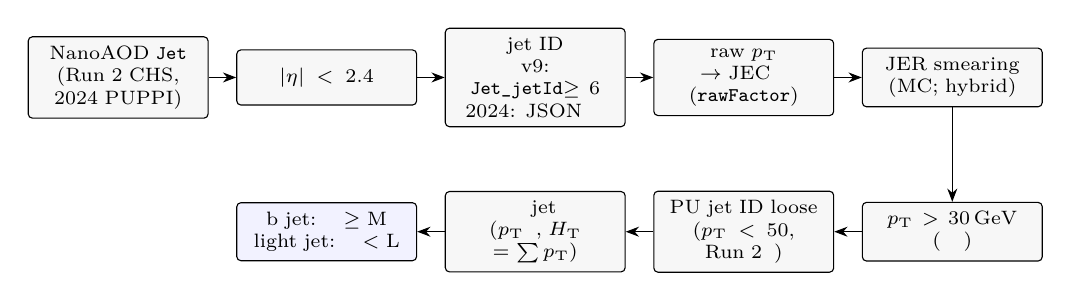
\begin{tikzpicture}[node distance=3.5mm and 3.5mm, every node/.style={font=\scriptsize},
  st/.style={draw,rounded corners=1.5pt,align=center,fill=black!3,minimum height=7mm,text width=2.05cm}, >=Stealth]
  \node[st] (a) {NanoAOD \texttt{Jet}\\ (Run 2 CHS, 2024 PUPPI)};
  \node[st,right=of a] (b) {$|\eta|<2.4$};
  \node[st,right=of b] (c) {jet ID\\ v9: \texttt{Jet\_jetId}$\geq 6$\\ 2024: JSON 재계산};
  \node[st,right=of c] (d) {raw \pt{} $\to$ JEC 다시\\ (\texttt{rawFactor})};
  \node[st,right=of d] (e) {JER smearing\\ (MC; hybrid)};
  \node[st,below=12mm of e] (f) {$\pt>30\GeV$\\ (보정 뒤)};
  \node[st,left=of f] (g) {PU jet ID loose\\ ($\pt<50$, Run 2 만)};
  \node[st,left=of g] (h) {선택 jet\\ (\pt{} 순, \HT{} = $\sum \pt$)};
  \node[st,left=of h,fill=blue!5] (i) {b jet: 점수 $\geq$ M\\ light jet: 점수 $<$ L};
  \draw[->] (a)--(b); \draw[->] (b)--(c); \draw[->] (c)--(d); \draw[->] (d)--(e); \draw[->] (e)--(f);
  \draw[->] (f)--(g); \draw[->] (g)--(h); \draw[->] (h)--(i);
\end{tikzpicture}
\caption{우리 jet 선택의 순서\,\src{ttHHanalyzer\_unified.cc, createObjects}. 2024 는 같은 청소 단계에서 jet veto map 의 사건 veto 를 더한다.}
\label{fig:objects-jetflow}
\end{figure}

\begin{itemize}
\item \textbf{순서}(그림~\ref{fig:objects-jetflow}): $|\eta|<2.4$ 를 먼저 보고(2024 jet ID payload 가 중앙 jet 만 보게), jet ID, raw \pt{}
  ($\pt(1-\texttt{rawFactor})$)에서 JEC 를 다시 곱하고, MC 는 JER 을 퍼뜨린 뒤 $\pt>30\GeV$ 를 건다. 질량도 같은 비율로 고친다. 다시 곱한
  JEC 와 ntuple 의 \pt{} 의 차이는 검증용으로 남긴다(\code{JEC_DiffRatio})\src{ttHHanalyzer\_unified.cc, createObjects}\tagimpl.
\item \textbf{JER}: gen jet 과 $\dR<0.2$ 이고 $|\pt-p_\text{T}^\text{gen}|<3\sigma_{\pt}\pt$ 이면 scaling, 아니면 $s>1$ 일 때만 stochastic
  (난수의 seed 는 run·lumi·event·jet 번호)\src{CorrectionsManager.cc, smearJER}\tagimpl.
\item \textbf{2017(v9)}: \texttt{Jet\_jetId} $\geq 6$(tight + TightLepVeto, \code{Cuts::jetID}), 보정 뒤 $\pt<50\GeV$ 이면 \texttt{Jet\_puId} $\geq 4$
  (loose, \code{Cuts::jetPUid}), b-tag 점수 \texttt{Jet\_btagDeepFlavB}\src{SelectionCuts.h; ttHHanalyzer\_unified.cc}\tagimpl.
\item \textbf{2024(v15)}: v15 에는 \texttt{Jet\_jetId} 가 없어 JME 의 \file{jetid.json.gz} 의 \code{AK4PUPPI_TightLeptonVeto} 로 다시 계산한다
  (v9 의 \texttt{Jet\_jetId} $\geq 6$ 과 같은 수준; 입력은 에너지 분율과 대전·중성 multiplicity). PUPPI 라 pileup ID 는 쓰지 않는다. b-tag 점수는
  \texttt{Jet\_btagUParTAK4B}, rho 는 \texttt{Rho\_fixedGridRhoFastjetAll}\src{STEP 24 §6; EraConfig.h}\tagimpl\tagrunthree.
\item \textbf{2024 jet veto map}: \file{jetvetomaps.json.gz} 의 \code{Summer24Prompt24_RunBCDEFGHI_V1}, type \texttt{jetvetomap}(파일 설명이
  data·MC 모두에 권고하는 map). NanoAOD $\pt>15\GeV$, tight ID, $\text{chEmEF}+\text{neEmEF}<0.9$, PF muon 과 $\dR>0.2$ 인 jet 이 veto 영역에
  있으면 사건을 버린다. 이 jet 조건은 JERC 권고를 기억으로 옮긴 것이라 확인이 필요하다\src{EraConfig.h, jetVetoMap; PLAN\_v15 §9.6 D11}.
  KNU smoke 에서 이 veto 가 사건의 23–25\,\%(TTHH 25\,\%, TTbar 23\,\%, Data 23\,\%)를 뺐다: jet 이 많은 사건이라 veto 영역에 걸릴 확률이
  크다\src{STEP 24 §12}\tagimpl\tagrunthree.
\item \textbf{분류}: 선택 jet 중 점수 $\geq$ M 은 b jet(\code{selectbJet}), 점수 $<$ L 은 light jet(\code{selectLightJet}, hadronic W 의
  후보)이다. \HT{} 는 선택 jet 의 \pt{} 의 합이다\src{ttHHanalyzer\_unified.cc, createObjects; ttHHanalyzer\_unified.h, selectJet}.
  WP 는 \ref{ch:btag} 장.
\end{itemize}

\begin{andiff}[jet 정의에서 Run 2 AN·ttH 와 다른 점]
(1) \textbf{lepton–jet 겹침 제거가 없다.} \code{createObjects} 의 jet 고리와 \code{event::selectJet} 에 lepton 과의 $\dR$ 검사가 없다(코드 검색으로
확인). FH 신호 영역은 lepton 을 veto 하므로 영향이 거의 없고, 고립된 lepton 이 지배하는 jet 은 TightLepVeto 가 대부분 뺀다. 그러나 lepton
제어영역에서는 lepton 을 포함한 jet 이 jet 수와 \HT{} 에 남을 수 있다\tagours. (2) 2024 는 PUPPI jet, JSON jet ID, jet veto map 으로
바뀐다\tagrunthree. (3) Run 2 는 AN 처럼 jet veto map 을 쓰지 않는다(AN 에 언급 없음; 최종 결과 전에 다시 볼 항목)\src{D-2026-10-02-C}.
(4) pileup ID 는 Run 2 의 모든 해에 \texttt{puId} $\geq 4$ 이다. AN 은 2016 표본에서 그 flag 의 뜻이 달라 \texttt{puId==1} 을 쓴다
\src{AN-22-122 v26, PDF p.44} --- 2016 을 켜기 전에 고칠 것.
\end{andiff}

\subsection{JES·JER 불확도, Run 2 v15}\label{sec:objects-jets-syst}

JES·JER 의 변형은 아직 없다. \code{sysName} 의 \code{kJES}, \code{kJER} 은 정의만 있고 JER 은 늘 \texttt{"nom"} 으로 부른다. 변형마다 사건을 다시
돌리는 경로(출력 디렉터리 따로)가 필요하다\src{PLAN\_ML\_SYST §5.1, §6}\tagplan. JEC 불확도 loader(\code{loadJECUncertainty_})는 있지만 생성자가
부르지 않는다\src{STATUS OPEN 6 P1}. AN 은 JES 를 ``11 scheme'' 의 출처를 모두 합친 하나로, JER 은 연도별 비상관으로 넣었다
\src{AN-22-122 v26, PDF p.120}(\ref{ch:syst} 장). 지금 analyzer 는 Run 2 를 v9 이름으로만 읽는다. v15 의 Run 2 를 읽으려면 jet ID 를 UL CHS
Tight + TightLepVeto 로 다시 계산하고(Y3: 같은 MiniAOD 의 v9·v15 2018 파일을 짝지어 v9 \texttt{Jet\_jetId} 와 대조), pileup ID 는
\texttt{Jet\_puIdDisc} 에 UL WP 임계값을 걸어야 한다(ROADMAP\_FH §3 의 C, D)\src{ROADMAP\_FH §3; PLAN\_v15 §2 \#1--2}\tagplan.

% -----------------------------------------------------------------------------
\section{Lepton: FH 의 veto 와 lepton 제어영역}\label{sec:objects-leptons}

\begin{table}[htbp]
\caption{lepton 정의(우리 코드)\,\src{ttHHanalyzer\_unified.cc, createObjects; SelectionCuts.h}. Run 3 는 전자 ID 이름만 다르다
(\texttt{Electron\_mvaIso\_WP90}).}
\label{tab:objects-leptons}
\centering\small
\begin{tabularx}{\textwidth}{@{}p{2.6cm}L L@{}}
\toprule
 & muon & 전자 \\
\midrule
veto(FH), 그리고 CR·SF 영역의 추가 lepton & $\pt>15\GeV$, $|\eta|<2.4$, tight ID, \texttt{pfRelIso04\_all} $<0.15$ &
$\pt>15\GeV$, $|\eta|<2.5$, $|\eta_\text{SC}|\notin[1.4442, 1.5660]$, MVA Fall17V2 iso WP90 \\
lead(lepton CR 의 gate) & 위 + $\pt>29\GeV$(\code{Cuts::leadMuonPt}) & 위 + $\pt>30\GeV$(\code{Cuts::leadElePt}) \\
\bottomrule
\end{tabularx}
\end{table}

\begin{itemize}
\item \textbf{FH 의 veto}: 표~\ref{tab:objects-leptons} 의 veto lepton 이 하나라도 있으면 버린다(\code{Cuts::nLeptons} = 0). 전자의 고립은
  MVA ID 에 들어 있어 따로 자르지 않는다\src{ttHHanalyzer\_unified.cc, createObjects}\tagimpl.
\item \textbf{비교}: ttHH AN 의 DL 차선행 muon 은 \texttt{pfRelIso04\_all} $<0.25$, 전자는 WP90, $\pt>15\GeV$, $|\eta|<2.5$ 이다
  \src{AN-22-122 v26, PDF p.42--44, Tables 33--35}. ttH(bb) FH 의 veto 는 muon isolation $<0.25$(PFIsoLoose), 전자는 cut-based tight,
  $|\eta|<2.4$ 이다\src{AN-19-094 v20, PDF p.54, Table 42}. 우리 veto muon 의 0.15 는 AN SL 의 선택 muon(PFIsoTight)과 같다
  \src{AN-22-122 v26, PDF p.40, Table 28}. Hbb 발표는 우리 정의를 ``DL subleading-lepton criteria'' 를 따른다고 적었지만 isolation 은
  DL(0.25)과 다르다\src{Hbb 회의 FH 발표 p.13}.
\item \textbf{lepton SF}: 아직 쓰지 않는다. lepton CR 의 수에는 그 예상 크기를 함께 적기로 했다\src{D-2026-10-02-D N4}\tagopen.
\end{itemize}

\subsection{lepton 제어영역(1 lepton + MET)}\label{sec:objects-lepcr}

\texttt{--region muon} 과 \texttt{--region electron} 은 lepton veto 단계를 ``그 flavour 의 lepton 정확히 1 개, 다른 flavour 0 개, $\MET>20\GeV$'' 로
바꾼다. 나머지 선택·trigger·Data PD 는 FH 와 같다(Data 는 강입자 PD)\src{STEP 14 §3; D-2026-10-02-D N5}\tagimpl. lepton 은 lead lepton
gate(muon 29, 전자 30\GeV)를 넘는 사건에서만 모으므로, 실제로는 lead lepton 하나와 $\pt>15$ 의 추가 lepton 없음이다
\src{ttHHanalyzer\_unified.cc, createObjects}. MET 는 Run 2 PF(Type-1) \texttt{MET\_pt}(v15 는 \texttt{PFMET\_pt}), 2024 \texttt{PuppiMET\_pt} 이고
\src{D-2026-10-02-D N3}, 우리가 다시 곱한 JEC·JER 은 MET 에 전파하지 않는다(NanoAOD 값 그대로)\src{ttHHanalyzer\_unified.cc, metPt\_}.

\begin{itemize}
\item \textbf{2017}: ``+1$\mu$, $\MET>20\GeV$'' 영역에서 Data 27,517, MC 35,380(tt 30,191, QCD 2,835)이었다. lepton 요구가 QCD 를 누르고
  Data/MC 를 거의 모든 곳에서 개선했지만 nb 와 함께 커지는 차이가 남았다\src{Hbb 회의 FH 발표 p.25--26}. jet 수 분포의 기울기도 남는다
  \src{D-2026-10-07-B}.
\item \textbf{2024}(SF 없음, 10-09): $\mu$CR 의 Data/MC 0.87(lepton 단계 뒤), 0.86(nb $\geq 2$), 1.19($\geq 3$), 1.41($\geq 4$), 0.84(마지막);
  eCR 0.80, 0.77, 1.07, 1.19, 0.75\src{STEP 26 §10}. 2024 CR 의 MC 에는 W$\to\ell\nu$·DY 표본이 없다(생산은 KNU 저장공간을 본 뒤)
  \src{D-2026-10-07-B; PLAN\_v15 §9.6 D13}\tagopen.
\end{itemize}

\begin{note}[왜 lepton 제어영역이 QCD data-driven 보다 먼저인가]
사용자의 방향은 ``QCD data driven 도 준비해야 한다. 단 이건 lepton selection 을 해서 적절한 data/MC ratio 가 나오면 하자'' 이다
\src{D-2026-10-10-B (6)}. 이유는 방법의 구조에 있다. ttH(bb) FH 식 추정은 낮은 b-tag 영역의 data 에서 \ttbar{} 등 MC 를 빼서 QCD 의
모양을 얻고, 신호 영역의 초기 정규화도 (data $-$ MC)로 잡는다\src{PLAN\_QCD\_DD §2.2, 결론 2}(\ref{ch:qcd} 장). 빼는 MC 가 틀리면 그 잘못이 QCD
template 으로 그대로 옮는다. 1 lepton + MET 영역은 QCD 가 눌려 \ttbar{} 가 지배하므로, 이 영역의 Data/MC 는 QCD 와 거의 무관하게
\ttbar{} 모델링과 trigger·b-tag SF 를 시험한다. 여기서 nb 나 jet 수에 따라 Data/MC 가 기울면, 그것은 QCD 만의 문제가 아니라 빼야 할 MC 의
문제이고, data-driven 방법이 그 기울기를 QCD 로 잘못 흡수하게 된다\tagours.
\end{note}

% -----------------------------------------------------------------------------
\section{사건 청소와 사건 weight}\label{sec:objects-cleaning}

D-2026-10-02-C 는 연도마다 모든 청소 항목에 값·출처·코드 위치를 두고, 항목을 빼려면 이유를 적게 했다(PLAN\_v15 §9.2 의 표가 단일
목록)\src{D-2026-10-02-C}. 표~\ref{tab:objects-cleaning} 이 지금 코드의 상태다.

\begin{table}[htbp]
\caption{연도별 사건 청소와 weight\,\src{EraConfig.h; CorrectionsManager.cc; PLAN\_v15 §9.2; AN-22-122 v26, PDF p.19, p.47--48, p.120}.}
\label{tab:objects-cleaning}
\centering\footnotesize
\begin{tabularx}{\textwidth}{@{}p{1.9cm}L L L@{}}
\toprule
항목 & ttHH AN(Run 2) & 우리 Run 2(2017 v9) & 우리 2024(v15) \\
\midrule
golden JSON & UL2017 등(Table 3) & \file{Cert_294927-306462_13TeV_UL2017_Collisions17_GoldenJSON.txt} & \file{Cert_Collisions2024_378981_386951_Golden.json}(2026-08-04 판, md5 확인) \\
PV & ndof $>4$, $|z|<24$ cm, $\rho<2$ cm, fake 아님 & \file{PV_npvsGood} $\geq 1$ & 같음 \\
MET filter & SL: 10 개 + ecalBadCalib(2017·18); DL: 8 개 + ecalBadCalib(2017·18) & DL 목록 9 개(ecalBadCalib 포함) & Run 3 목록 8 개(HBHE 둘 빠짐, hfNoisyHits 더함; 기억 → 확인) \\
jet veto map & 없음 & 없음 & \texttt{jetvetomap}, 사건 veto \\
HEM(2018) & JES 변형 20/35\,\%, 영향 무시 & 영역만 정의, 적용 안 함 & --- \\
L1 prefiring & 2016·2017(본문은 rate, Table 53 은 shape 계통) & \file{L1PreFiringWeight_Nom}(Up/Dn 은 Tree) & 없음(branch 도 없음) \\
pileup & $\sigma_\text{mb}\pm4.6\,\%$ & LUM \file{Collisions17_UltraLegacy_goldenJSON}(up/down Tree) & 우리 JSON \file{Collisions24_goldenJSON}(up/down Tree) \\
\bottomrule
\end{tabularx}
\end{table}

\begin{itemize}
\item \textbf{MET filter}: Run 2 목록은 \code{Flag_goodVertices}, \code{globalSuperTightHalo2016Filter}, \code{HBHENoiseFilter},
  \code{HBHENoiseIsoFilter}, \code{EcalDeadCellTriggerPrimitiveFilter}, \code{BadPFMuonFilter}, \code{BadPFMuonDzFilter}, \code{eeBadScFilter},
  \code{ecalBadCalibFilter} 로 AN DL 의 Table 42 와 같다. AN SL(Table 40)은 \code{hfNoisyHitsFilter} 와 \code{BadChargedCandidateFilter} 를 더
  쓴다\src{EraConfig.h, metFilters; AN-22-122 v26, PDF p.47--48}. 2024 의 Run 3 목록은 HBHE 둘을 빼고 \code{hfNoisyHitsFilter} 를 더한 8 개이고
  JME 권고로 확인할 항목이다\src{PLAN\_v15 §9.2}\tagrunthree. 2024 는 jet veto map 을 같은 청소 단계에 넣고 둘을 따로 센다
  (\texttt{[cleaning]} 줄)\src{STEP 24 §6}.
\item \textbf{L1 prefiring}: 2016·2017 MC 에 \code{L1PreFiringWeight_Nom} 을 곱한다. 그 해에 값이 0 이하이면(branch 가 없다는 뜻) FATAL 이다
  --- 연도 게이트 없이 곱하면 branch 가 없는 2018 v9 에서 모든 MC weight 가 0 이 되기 때문이다\src{ttHHanalyzer\_unified.cc, process}.
  Up/Dn 은 Tree v1 에 기록한다\src{STEP 27 §O.4}. 2018 v15 에는 branch 가 있어 muon 성분을 쓸지가 열려 있다\src{PLAN\_v15 §7 D9}\tagopen.
\item \textbf{HEM(2018)}: AN 은 2018 MC 에 HEM 영역 jet 의 에너지를 20\,\%·35\,\% 바꾼 JES 변형을 보았고 영향이 무시할 만하다고 했다
  \src{AN-22-122 v26, PDF p.120}. \code{EraConfig::hemJes} 에 영역만 정의되어 있다\tagplan.
\item \textbf{pileup}: Run 2 는 jsonpog LUM payload. 2024 는 jsonpog 에 LUM 이 없어 직접 만들었다: data 는 DQM 의 공식 히스토그램
  \file{dataPileupHistogram-2024CDEFGHI_Golden-69200ub.root}(중앙, 평균 50.03; 66000/72400 ub 가 down/up, $\pm4.6\,\%$), MC 는 skim 하지 않은
  Summer24 ZZ 파일럿(4,800,000 사건)의 \file{Pileup_nTrueInt} 이다. 우리 2024 표본은 jet 6 개 skim(\texttt{6j20})이라 pileup 이 높은 사건이 더
  남으므로 그 분포를 쓰지 않았다. 히스토그램의 LS 집합은 우리 golden JSON 과 lumi 로 0.2\,\% 다르다. 결과는
  \file{DerivedCorr/PU/2024_Summer24/puWeights_2024.json}\src{D-2026-10-05-A; DerivedCorr/PU/2024\_Summer24/README.md}\tagimpl\tagrunthree.
\item \textbf{사건 weight}: MC 는 $w = \frac{L\sigma B k}{\sum w_\text{gen}}\, w_\text{gen}\, w_\text{PU}\, w_\text{L1}\, w_\text{stitch}$ 에 SF 를
  곱한다(식~\eqref{eq:trigger-weight}); $k=1$ 이다. Data 는 1 이고 golden JSON 밖의 사건은 버린다\src{STEP 14 §4; ttHHanalyzer\_unified.cc, process}.
\end{itemize}

\begin{table}[htbp]
\caption{연도별 correctionlib payload(지금 코드)\,\src{CorrectionsManager.cc, loadJME\_/loadPU\_/loadBTag\_/loadRun3Jet\_; EraConfig.h; PLAN\_v15 §9.2}.}
\label{tab:objects-payloads}
\centering\footnotesize
\begin{tabularx}{\textwidth}{@{}p{1.5cm}L L@{}}
\toprule
 & 2017 UL(2018 UL 은 \texttt{UL17}$\to$\texttt{UL18}) & 2024 \\
\midrule
JEC & \file{Summer19UL17_V5_MC_L1L2L3Res_AK4PFchs}; Data \file{Summer19UL17_Run<era>_V5_DATA_...} & \file{Summer24Prompt24_V1_MC/DATA_L1L2L3Res_AK4PFPuppi}(DATA 는 입력 \texttt{run}) \\
JER & \file{Summer19UL17_JRV2_MC_PtResolution/ScaleFactor_AK4PFchs} & \file{Summer23BPixPrompt23_RunD_JRV1_MC_..._AK4PFPuppi}(2023 BPix 의 것) \\
jet ID·veto & NanoAOD \file{Jet_jetId} & \texttt{jetid.json.gz}: \file{AK4PUPPI_TightLeptonVeto}; \texttt{jetvetomaps.json.gz} \\
pileup & \file{POG/LUM/2017_UL/puWeights.json.gz} & \file{DerivedCorr/PU/2024_Summer24/puWeights_2024.json} \\
b-tag & \file{POG/BTV/2017_UL/btagging.json.gz}: \file{deepJet_shape} & \file{btagging_preliminary.json.gz}: \file{UParTAK4_kinfit} \\
\bottomrule
\end{tabularx}
\end{table}

payload 의 입력 순서는 payload 가 선언한 이름으로 맞춘다(2024 MC JEC 는 \texttt{JetPhi}, DATA 는 \texttt{run} 이 더 있다)\src{STEP 24 §6}.
Data 의 JEC 키를 못 찾으면 MC JEC 로 대신하지 않고 멈춘다\src{CorrectionsManager.cc, loadJME\_}.

% -----------------------------------------------------------------------------
\section{객체 요약표}\label{sec:objects-summary}

표~\ref{tab:objects-summary} 는 이 장의 정의를 Run 2 ttHH AN, ttH(bb) FH 와 나란히 놓는다. 크게 다른 곳은 lepton–jet 겹침 제거, veto muon 의
isolation, 2024 의 jet 종류와 b-tagger 이다.

\begin{center}\begin{minipage}{\textwidth}
\captionof{table}{객체 정의의 비교. ttHH AN 은 SL·DL, ttH 는 AN-19-094 의 FH\,\src{AN-22-122 v26, PDF p.39--45; AN-19-094 v20, PDF p.54--58;
SelectionCuts.h; EraConfig.h; ttHHanalyzer\_unified.cc}.}
\label{tab:objects-summary}
\centering\scriptsize
\renewcommand{\arraystretch}{1.18}
\begin{tabularx}{\textwidth}{@{}>{\raggedright\arraybackslash}p{1.4cm}L L L L@{}}
\toprule
 & ttHH AN (SL / DL) & ttH(bb) FH & 우리 2017 (v9) & 우리 2024 (v15) \\
\midrule
jet & AK4 CHS, $\pt>30$, $|\eta|<2.4$, TightLepVeto, PU ID loose ($\pt<50$), $\dR(\ell,j)<0.4$ 제거 & 같음 & 같음, 단 $\dR(\ell,j)$ 제거 없음 & AK4 PUPPI, $\pt>30$, $|\eta|<2.4$, JSON TightLepVeto, PU ID 없음, veto map \\
JEC / JER & \file{Summer19UL17_V5} / \texttt{JRV2} (2017) & 연도별 Table 49 & AN 과 같음(다시 곱함, hybrid JER) & \file{Summer24Prompt24_V1} / \texttt{Summer23BPix...JRV1} \\
b-tag & DeepJet M (L 은 DL 의 loose 범주) & DeepJet M, CR 에 L & DeepJet M 0.3040, L 0.0532 & UParTAK4 M 0.1272, L 0.0246 \\
veto / 차선행 $\mu$ & SL veto: iso $<0.15$; DL: iso $<0.25$, $\pt>15$ & tight, iso $<0.25$, $\pt>15$ & tight, iso $<0.15$, $\pt>15$ & 같음 \\
veto / 차선행 e & SL: 같은 MVA ID 의 veto WP, $\pt>15$; DL: WP90, $\pt>15$, $|\eta|<2.5$ & cut-based tight, $|\eta|<2.4$ & WP90, $\pt>15$, $|\eta|<2.5$ & 같음(\file{mvaIso_WP90}) \\
선택 lepton & SL $\mu$ 26/29/26, e 29/30/30; DL 25/15 & --- (veto 만) & CR gate $\mu$ 29, e 30 & 같음 \\
MET & SL $>20$, DL $>40$ & 요구 없음 & CR 만 $>20$ (PF) & CR 만 $>20$ (PUPPI) \\
\bottomrule
\end{tabularx}\end{minipage}
\end{center}

% -----------------------------------------------------------------------------
\section{변경 이력}\label{sec:objects-history}

\begin{center}\begin{minipage}{\textwidth}
\captionof{table}{객체·보정의 변경 이력.}
\label{tab:objects-history}
\small
\begin{tabularx}{\textwidth}{@{}>{\raggedright\arraybackslash}p{3.3cm}L@{}}
\toprule
날짜·기록 & 내용 \\
\midrule
2026-06-15 STEP 14 & lepton CR(\texttt{--region muon|electron}, 1 lepton + $\MET>20\GeV$) \\
2026-07-29 CHANGELOG & 연도 의존 상수를 \file{EraConfig.h} 로(L1 prefiring 게이트, golden JSON 파일 이름, 2018 Data JEC 의 era) \\
2026-10-02 D-2026-10-02-B·C·D & 무음 0 금지(필수 branch 검사), 연도별 청소 목록, MET 은 Run 2 PF·2024 PUPPI(N3), lepton SF 는 처음엔 안 씀(N4) \\
2026-10-05 STEP 24, D-2026-10-05-A & 2024: PUPPI·JSON jet ID·jet veto map·Run 3 MET filter·v15 이름, 2024 PU weight(DQM 히스토그램) \\
2026-10-07 D-2026-10-07-B & 2024 lepton CR 을 FH 와 함께 실행, W$\to\ell\nu$·DY 생산은 저장공간을 본 뒤 \\
2026-10-10 STEP 27(O), D-2026-10-10-B & PU·L1 prefiring up/down, MET $\phi$, jet $\phi$·질량을 Tree v1 에; QCD data-driven 은 lepton CR 뒤 \\
\bottomrule
\end{tabularx}\end{minipage}
\end{center}

% -----------------------------------------------------------------------------
\section{미결 사항}\label{sec:objects-open}

\begin{openq}
\begin{enumerate}
\item \textbf{lepton–jet 겹침 제거}: AN·ttH 처럼 선택 lepton 과 $\dR<0.4$ 인 jet 을 뺄지(특히 lepton CR) --- 넣으면 FH 와 CR 의 jet 정의가 AN 과
  같아진다\tagours.
\item \textbf{veto muon isolation}: 0.15(지금) 대 0.25(AN DL 차선행, ttH FH veto). 0.15 이면 isolation 0.15–0.25 의 muon 이 있는 사건이 FH 에 남아
  DL 과 겹칠 수 있다(SL·DL·FH 결합 때 세 채널의 직교성을 표로 확인할 것)\tagours.
\item \textbf{2024 jet veto map}: veto 에 쓰는 jet 조건과 \texttt{\_bpix}·\texttt{\_fpix} type 을 더 쓸지 JERC 권고로 확인; 23–25\,\% 수용도 손실의
  신호 민감도 영향\src{PLAN\_v15 §9.6 D11}.
\item \textbf{Run 3 MET filter 목록}과 \texttt{jetid.json} 의 2024 전용 기준 확인(파일 설명은 ``Run3 Rereco2022CDE'')\src{STEP 24 확인하지 못한 것}.
\item \textbf{JES·JER 변형}(sysType 배선, 변형 실행)과 JEC 불확도 loader; 2018 HEM 변형\tagplan.
\item \textbf{lepton SF}(CR 정규화)와 2024 W$\to\ell\nu$·DY 표본(D13).
\item \textbf{2016}: \file{CorrectionsManager.cc} 의 2016 JEC/JER 키가 AN Table 30 과 다르다(MC 는 preVFP 도 \texttt{Summer19UL16\_V7},
  JER 은 \texttt{Summer19UL16\_JRV2}; Data 키는 era 와 상관없이 \texttt{Summer19UL16APV\_RunFGH\_V7})\src{CorrectionsManager.cc, loadJME\_}.
  2016 은 아직 켜지 않으므로 결과에는 영향이 없지만 켜기 전에 고칠 것. MET filter 의 \texttt{ecalBadCalib} 도 AN 에서는 2016 에 없다.
\item \textbf{PV}: \texttt{PV\_npvsGood} 의 정의가 AN 의 PV 기준과 같은지 이 문서의 출처로는 확인 못 함.
\end{enumerate}
\end{openq}

% =============================================================================
% 5 장 b-tagging 과 b-tag SF  (AN_KR v0.1, 2026-10-10)
% 출처: AN-22-122 v26 §5.2.4, §5.3.4, §8.2.1, App. D; AN-19-094 v20 §4.6, §9, App. A;
%       Hbb 회의 FH 발표, KCMS 발표; tempTTHH STEP 14·16·24·25·26·27, CHANGELOG 2026-07-29 (2);
%       DECISIONS(D-2026-10-02-D N7·N8, D-2026-10-08-A, D-2026-10-10-A·B), PLAN_v15 §9.2·§9.6 D10, PLAN_ML_SYST §5–6·§9;
%       코드(EraConfig.h, BTagEffGroup.h, CorrectionsManager.cc, ttHHanalyzer_unified.{h,cc},
%       bTagSF_ReweightStudy/, tools/stage7/btag_eff_maps.py)
% =============================================================================
\chapter{b-tagging 과 b-tag SF}\label{ch:btag}

ttHH($\to$4b) 의 신호는 b quark 6 개를 가지므로 b-tag 은 신호 영역의 정의(b jet 수)와 배경 분리의 중심이다. Run 2 는 DeepJet 판별값의
분포 전체를 jet 마다 data 에 맞추는 shape SF 를 쓰고, 그 SF 가 바꾼 b-tag 요구 전의 수율을 과정 묶음마다 jet 수 $\times$ \HT{} 의 함수로
되돌리는 normalisation reweight 를 곱한다(AN 과 ttH(bb) 의 방법). 2024 는 BTV 가 UParTAK4 의 b jet fixed-WP SF 만 주므로, 우리 선택이
쓰는 두 WP(L, M)로 BTV ``method 1a'' 의 사건 weight 를 만들고 MC 효율 맵은 우리가 만든다. 2026-10-10 에 BTV 의 다중 WP 안내에 맞춰
L–M 구간 인자의 음수 분자를 1 로 바꾸고, 참 b jet 수별 closure 와 비교 weight 둘을 기록하게 했다. 2024 의 shape SF 와 c jet 의 처리는
BTV 의 답을 기다린다.

% -----------------------------------------------------------------------------
\section{b-tagging 의 원리와 SF}\label{sec:btag-theory}

\paragraph{b jet 의 특징.}
b hadron 은 수명이 ps 규모라서 실험실계에서 mm 정도 날아간 뒤 붕괴하고, 질량이 커서 붕괴 산물이 많다. 그래서 b jet 에는 (1) 1차 정점에서
떨어진 궤적(큰 impact parameter 와 그 유의도), (2) 질량과 궤적 수가 큰 2차 정점, (3) 반렙톤 붕괴에서 오는 jet 안의 부드러운 lepton 이 있다.
c hadron 도 같은 특징을 약하게 가져서 c jet 이 가장 어려운 mistag 이다. MC 에서 jet 의 맛(flavour)은 hadron 기준(\texttt{Jet\_hadronFlavour}:
b hadron 이 jet 에 묶이면 5, c 이면 4, 아니면 0)으로 정하고, 우리 코드의 SF·효율은 모두 이 값을 쓴다
\src{ttHHanalyzer\_unified.cc, createObjects}.

\paragraph{tagger.}
CMS 의 tagger 는 이런 변수를 사람이 고르던 방식에서 jet 구성 입자의 목록을 그대로 읽는 신경망으로 옮겨 왔다: Run 2 의 DeepJet
(\texttt{Jet\_btagDeepFlavB}), Run 3 의 graph·transformer 계열이다. 우리 2024 는 UParTAK4(\texttt{Jet\_btagUParTAK4B})를 쓴다
\src{EraConfig.h, btagWP}. 출력은 맛별 확률이고, b 판별값 하나에 문턱을 걸거나(WP) 판별값 분포 전체를 쓴다.

\paragraph{working point(WP).}
WP 는 light jet 의 mistag 비율이 정해진 값이 되는 판별값 문턱이다. DeepJet 의 loose/medium/tight 는 $\pt\approx80\GeV$ 의 non-b jet 에서
mistag 약 10\,\%, 1\,\%, 0.1\,\% 에 해당한다\src{AN-22-122 v26, PDF p.44}. 표~\ref{tab:btag-wp} 가 우리가 쓰는 값이다. 우리 선택에서
b jet 은 점수 $\geq$ M, hadronic W 의 light jet 은 점수 $<$ L 이다\src{ttHHanalyzer\_unified.cc, createObjects}. ttHH AN 의 DL 도
medium, ``loose 이고 medium 아님'', ``loose 실패''(light)의 세 범주를 쓴다\src{AN-22-122 v26, PDF p.42, Table 33; PDF p.45, Table 37}.

\begin{table}[htbp]
\caption{우리 코드의 b-tag WP\,\src{EraConfig.h, btagWP; AN-22-122 v26, PDF p.41, Table 32; PLAN\_v15 §9.2}.}
\label{tab:btag-wp}
\centering\small
\begin{tabular}{@{}lllll@{}}
\toprule
연도 & tagger(branch) & L & M & T \\
\midrule
2016 preVFP & DeepJet(\texttt{btagDeepFlavB}) & 0.0508 & 0.2598 & 0.6502 \\
2016 postVFP & DeepJet & 0.0480 & 0.2489 & 0.6377 \\
2017 & DeepJet & 0.0532 & 0.3040 & 0.7476 \\
2018 & DeepJet & 0.0490 & 0.2783 & 0.7100 \\
2024 & UParTAK4(\texttt{btagUParTAK4B}) & 0.0246 & 0.1272 & 0.4648 (XT 0.6298, XXT 0.9739) \\
\bottomrule
\end{tabular}
\end{table}

\paragraph{왜 data 와 MC 가 다른가, 그리고 SF.}
tracking 의 효율과 정렬, impact parameter 분해능, b·c 의 fragmentation 과 붕괴, gluon splitting, pileup 은 시뮬레이션이 완벽하지 않다. 그래서
같은 WP 의 효율이 data 와 MC 에서 다르고, 판별값 분포의 모양도 다르다. 두 종류의 SF 가 있다:
\begin{itemize}
\item \textbf{fixed-WP SF}: $\mathrm{SF}_X(f,\pt,\eta) = \varepsilon_X^\text{data}/\varepsilon_X^\text{MC}$ ($X$ = WP, $f$ = 맛). 사건 weight 를
  만들려면 MC 효율 $\varepsilon_X^\text{MC}$ 이 따로 필요하다(\S\ref{sec:btag-fixedwp}).
\item \textbf{shape(reshaping) SF}: jet 마다 판별값 $D$ 의 함수 $\mathrm{SF}(D; f,\pt,\eta)$ 로, MC 의 $D$ 분포를 data 의 것으로 바꾼다. HF·LF 가
  많은 제어 표본에서 다른 맛의 기여를 빼 가며 번갈아 맞추는 iterative fit(tag-and-probe)으로 만들고\src{AN-19-094 v20, PDF p.59, p.154}, 불확도는 \S\ref{sec:btag-run2} 의 출처들로 나뉜다.
  MC 효율 맵이 필요 없고 모든 WP 와 판별값을 쓰는 입력 변수가 함께 고쳐진다.
\end{itemize}

\begin{figure}[htbp]
\centering
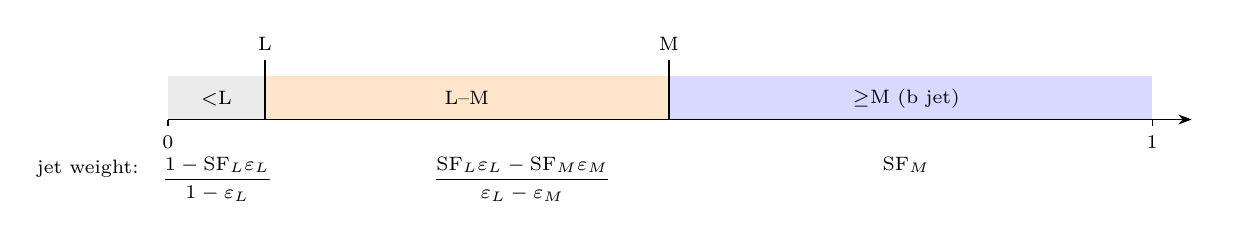
\begin{tikzpicture}[x=12.5cm,y=1cm,>=Stealth]
  \fill[black!8]  (0,0) rectangle (0.0246*4,0.55);
  \fill[orange!20] (0.0246*4,0) rectangle (0.1272*4,0.55);
  \fill[blue!15]  (0.1272*4,0) rectangle (1,0.55);
  \draw[->] (0,0) -- (1.04,0) node[right,font=\scriptsize] {점수};
  \draw (0,0) -- (0,-0.08) node[below,font=\scriptsize] {0};
  \draw (1,0) -- (1,-0.08) node[below,font=\scriptsize] {1};
  \draw[thick] (0.0246*4,0) -- (0.0246*4,0.75) node[above,font=\scriptsize] {L};
  \draw[thick] (0.1272*4,0) -- (0.1272*4,0.75) node[above,font=\scriptsize] {M};
  \node[font=\scriptsize,align=center] at (0.0246*2,0.27) {$<$L};
  \node[font=\scriptsize,align=center] at (0.0246*4/2+0.1272*4/2,0.27) {L–M};
  \node[font=\scriptsize,align=center] at (0.75,0.27) {$\geq$M (b jet)};
  \node[font=\scriptsize,align=center,below] at (0.05,-0.35) {$\dfrac{1-\mathrm{SF}_L\varepsilon_L}{1-\varepsilon_L}$};
  \node[font=\scriptsize,align=center,below] at (0.36,-0.35) {$\dfrac{\mathrm{SF}_L\varepsilon_L-\mathrm{SF}_M\varepsilon_M}{\varepsilon_L-\varepsilon_M}$};
  \node[font=\scriptsize,align=center,below] at (0.75,-0.35) {$\mathrm{SF}_M$};
  \node[font=\scriptsize,left] at (-0.02,-0.62) {jet weight:};
\end{tikzpicture}
\caption{두 WP(L, M)가 나누는 세 칸과 2024 fixed-WP 방법의 jet weight(식~\eqref{eq:btag-method1a}). 칸의 너비는 눈금을 4 배로 늘린
개념도이다(2024 UParTAK4 의 L 0.0246, M 0.1272).}
\label{fig:btag-bins}
\end{figure}

% -----------------------------------------------------------------------------
\section{Run 2: shape SF 와 b-tag normalisation reweight}\label{sec:btag-run2}

\subsection{Run 2 AN 과 ttH(bb) 의 방법}\label{sec:btag-run2-an}

ttHH AN 의 SL 은 여러 DNN 입력이 DeepJet 점수로 만들어지므로 값보다 모양의 data/MC 차이가 중요하다고 보고 BTV 의 DeepJet shape SF 를
골랐다. correctionlib 으로 jet 마다 SF(맛, $\eta$, \pt, 판별값)를 읽고 사건 weight 는 선택된 모든 jet 의 곱이다\src{AN-22-122 v26, PDF p.41}:
\begin{equation}
  \omega_\text{evt} = \prod_{i\,\in\,\text{jets}} \mathrm{SF}(D_i, p_{\mathrm{T},i}, \eta_i;\, f_i).
  \label{eq:btag-shape-weight}
\end{equation}
불확도의 출처는 ``lf'', ``hf'', ``hfstats1'', ``hfstats2'', ``lfstats1'', ``lfstats2'' 를 b jet 과 light jet 에 함께, c jet 에는
``cferr1'', ``cferr2'' 를 걸고, ``jes'' 는 JES 를 움직인 사건에 함께 건다\src{AN-22-122 v26, PDF p.41, p.121}. 각 출처의 뜻은 ttH(bb) AN 이
설명한다\src{AN-19-094 v20, PDF p.153--154}:
\begin{itemize}
\item \textbf{hf, lf(purity)}: SF 를 유도한 제어 표본에 섞인 다른 맛(HF 표본의 LF, LF 표본의 HF)의 양을 바꿨을 때의 SF 변화. 유도가 반복적이라
  다른 맛의 SF 도 조금 움직인다.
\item \textbf{hfstats1/2, lfstats1/2}: 제어 표본의 통계. 1 차(linear)는 판별값 분포 전체의 기울기, 2 차(quadratic)는 양 끝이 가운데에 대해
  움직이는 변형이다. 표본이 해마다 독립이므로 연도 간 비상관이다.
\item \textbf{cferr1/2}: c jet 의 SF 는 1 로 두고 HF SF 의 상대 불확도를 두 배로 키워 두 nuisance 로 만든다.
\item \textbf{jes}: JES 가 움직이면 SF 의 입력(\pt)이 움직이므로 JES 변형과 함께 한다.
\end{itemize}
상관은 AN 본문이 ``hf/lf stats1/2 는 연도 간 비상관, hf/lf·cferr1/2 는 상관''\src{AN-22-122 v26, PDF p.120--121} 이라 하지만 SL 의 impact
그림에는 \texttt{CMS\_btag\_hf\_2016/2017/2018} 처럼 연도별 이름이 있다\src{AN-22-122 v26, PDF p.128, Fig. 100}. ttH(bb) 는 purity·charm 을
2017–2018 상관, 2016 은 따로 두었다\src{AN-19-094 v20, PDF p.154}.

\paragraph{jet 마다 어느 변형을 거는가(BTV 의 recipe).}
사건의 출처 $s$ 변형 weight 는 jet 마다 아래 규칙으로 고른 SF 의 곱이다. payload 가 출처마다 각 맛에 무엇을 하는지 이미 알고 있으므로
(예: ``hf'' 는 light jet 의 SF 도 조금 바꾼다), 규칙은 c jet 과 c 아닌 jet 의 구분뿐이다.
\begin{center}\small
\begin{tabular}{@{}lll@{}}
\toprule
jet 의 맛 & $s\in\{$hf, lf, hfstats1/2, lfstats1/2, jes$\}$ & $s\in\{$cferr1, cferr2$\}$ \\
\midrule
b(5), light(0) & $\mathrm{SF}_{s,\pm}$ & 중앙값 \\
c(4) & 중앙값 & $\mathrm{SF}_{s,\pm}$ \\
\bottomrule
\end{tabular}
\end{center}

\paragraph{normalisation reweight.}
SL 은 SF 전후의 사건 수가 같도록 $R = \sum\omega_\text{before}/\sum\omega_\text{after}$ 를 b-tag 요구 없이 측정했다. 처음에는 중앙 SF 로 구한
인자 하나를 모든 변형에 썼지만 lf·cferr 등에서 수 \% 의 수율 차이가 남아 변형마다 따로 측정했다\src{AN-22-122 v26, PDF p.41--42, p.170}.
과정(ttHH, ttH(SL), tt(SL), ttbb(SL), tt4b)과 연도마다 따로이고(App.~D), 본문은 이를 ``jet multiplicity correction'' 이라 부른다. 측정
위상공간은 본문에 따라 jet 4 개 이상(§5.2.4), 5 개 이상(§8.2.1), b-tag 을 뺀 baseline(App.~D)으로 다르게 적혀 있다\src{AN-22-122 v26, PDF p.41,
p.121, p.170}. DL 은 jet 수와 \HT{} bin 에서 변형마다 정규화를 맞췄다\src{AN-22-122 v26, PDF p.45}. ttH(bb) 는 SF 뒤에 jet 수와 \HT{} 분포가
b-tag 요구 전과 달라지는 것(2017 이 가장 큼)을 보고, 과정(ttH, tt+bb, tt+cc, tt+LF; 작은 배경은 tt+LF 값)마다 (jet 수, \HT) 의 함수인
``b-tag SF patch'' 를 b-tag 요구를 뺀 baseline 에서 유도해 곱했다\src{AN-19-094 v20, PDF p.59--60}.

\begin{note}[shape SF 가 왜 b-tag 요구 전의 수율을 바꾸는가]
맛·\pt·$\eta$ 가 같은 jet 들에서 SF 의 MC 평균 $\langle\mathrm{SF}\rangle = \int \mathrm{SF}(D)\,p_\text{MC}(D)\,dD$ 를 생각하자. shape SF 는 판별값의
모양을 맞추도록 유도한 것이고 정규화는 유도한 표본의 것이므로, 분석의 위상공간(jet 구성, 운동학, 맛의 비율이 다름)에서는
$\langle\mathrm{SF}\rangle = 1+\delta$ 가 1 이 아닐 수 있다. jet 들이 독립이면 사건 weight 의 기댓값은
\begin{equation}
  \mathbb{E}[\omega_\text{evt}] = \prod_{i=1}^{N_j} \langle\mathrm{SF}\rangle_i \approx (1+\bar\delta)^{N_j} \approx 1 + N_j\bar\delta
  \label{eq:btag-shape-bias}
\end{equation}
로 jet 수와 함께 커진다. 그래서 b-tag 을 요구하지 않은 수율이 바뀌고 jet 수와 \HT{} 의 분포가 기운다. 이 효과는 SF 가 고치려는 것(b-tag 된
사건의 비율과 판별값 모양)이 아니므로, b-tag 요구 전의 수율을 jet 수(와 \HT)의 함수로 되돌린다. 변형마다 $\bar\delta$ 가 다르므로 인자도
변형마다 다시 구한다(AN SL 의 결론과 같다). 되돌린 뒤에도 b-tag 된 사건의 비율과 점수 모양의 보정은 남는다.
\end{note}

\subsection{우리 FH 분석에서는}\label{sec:btag-run2-ours}

\begin{itemize}
\item \textbf{payload}: \file{POG/BTV/2017_UL/btagging.json.gz} 의 \code{deepJet_shape}(입력 systematic, flavor, $|\eta|$, \pt, 판별값; $|\eta|$ 는
  [0, 2.4999], \pt{} 는 [20, 1000]\GeV, 판별값은 [0, 1] 로 자른다). 함수는 c jet 에 cferr 아닌 변형이, c 아닌 jet 에 cferr 변형이 들어오면 중앙값을
  쓴다\src{CorrectionsManager.cc, loadBTag\_, getBTagSF\_Shape}\tagimpl.
\item \textbf{중앙 weight}: \code{computeBTagWeight} 가 모든 MC 사건에서 선택 jet 의 SF 를 곱해 \code{bTagWeight} 를 만든다(cut-flow 사슬이
  쓴다)\src{ttHHanalyzer\_unified.cc, computeBTagWeight}\tagimpl.
\item \textbf{출처별 weight}: \code{computeBTagShapeVariations_} 가 Tree 에 들어가는 사건에서만 위 recipe 로 8 출처 $\times$ up/down = 16 개를
  계산해 \code{bTagWeight_<src>_up/_down} 에 쓴다(jes 는 JES 변형 실행과 함께, 아직 없음). STEP 27 전의 analyzer 는 hf 를 b jet 에만, lf 를
  light jet 에만 걸었는데 그 값은 어디에도 기록되지 않아 결과에는 영향이 없었다. \file{bTagSF_ReweightStudy} 의
  \code{resolveJetSystematic} 은 처음부터 같은 BTV 규칙이었다\src{STEP 27 결론 4, §O.5}\tagimpl\tagtest.
\item \textbf{norm reweight 의 정의}(\file{bTagSF_ReweightStudy/}): 과정 묶음 $g$, jet 수 $n_j$, \HT{} 의 bin 마다
  \begin{equation}
    r_g(n_j, H_\mathrm{T}) = \frac{\sum_{\text{evt}\in g,\,\text{bin}} \omega_\text{base}\,\mathrm{SF}_\text{trig}}{\sum_{\text{evt}\in g,\,\text{bin}} \omega_\text{base}\,\mathrm{SF}_\text{trig}\,\omega_\text{evt}},
    \qquad
    w = \omega_\text{base}\cdot\mathrm{SF}_\text{trig}\cdot\omega_\text{evt}\cdot r_g(n_j, H_\mathrm{T})
    \label{eq:btag-normrw}
  \end{equation}
  이다\src{Hbb 회의 FH 발표 p.23}\src{BTagSFProcessor.cpp, Loop}. $\omega_\text{base}$ = genWeight $\times$ PU $\times$ L1 prefiring $\times$ stitch $\times$ (단면적 weight)
  이다. 발표의 $r_g$ 식은 합에 trigger SF 를 적지 않았지만 코드는 분자·분모의 사건 weight 에 함께 곱한다. 사건은 btagtrig skim 에서 강입자 trigger 를
  통과하고 측정 영역(기본 \texttt{FH}: \texttt{nVetoLeptons == 0}; 선택 \texttt{muonCR})에 든 것, b-tag 요구는 없다\src{BTagSFProcessor.cpp, Loop; Config.hh}\tagimpl.
\item \textbf{묶음과 bin}: tt+LF, tt+cc, tt+B, tt+nb, ttH, ttHH, ttZH4b, ttZZ4b 의 8 묶음. inclusive \ttbar{} 는 사건마다 확장한
  \texttt{genTtbarId} 로 나누고, QCD·V+jets·single top·VV·ttV 같은 작은 배경은 ttH(bb) 처럼 tt+LF 값을 쓴다. jet 수는 0–25(넘으면 마지막 bin),
  \HT{} 경계는 500, 550, 600, 700, 800, 1000, 1100, …, 1800, 2100, 2500\GeV(범위 밖 clamp), 빈 bin 은 1 이다. 변형 키는 central 과
  up/down $\times$ \{lf, hf, hfstats1/2, lfstats1/2, cferr1/2, jes\} 의 19 개다\src{Config\_TtCatGroup.hh; Config.hh; makeReweightJSON.cpp}\tagimpl.
  출력은 correctionlib JSON \file{btagNormReweight.json}(묶음 8 개)이다\src{Hbb 회의 FH 발표 p.43}.
\item \textbf{analyzer 의 적용}: \HT{} 단계에서 \code{getBTagReweight("central", processKey, nJets, HT)}; production weight 에는
  \texttt{--btagrw on} 일 때만 곱하고(기본 off) \code{evtWeight_full} 에는 늘 곱한다. 지금은 중앙값만 쓴다; 변형별 인자는 JSON 에 있고
  Tree 의 출처별 weight 에 downstream 이 곱하기로 했다\src{STEP 27 §O.4; STEP 16 §1}\tagimpl.
\item \textbf{2017 의 상태}: 2026-07-29 에 유도 사슬의 무음 오류를 고쳤다(묶음을 확장 \texttt{genTtbarId} 로, \texttt{stitchWeight} 를 곱함,
  측정 영역에 lepton 조건)\src{CHANGELOG 2026-07-29 (2)}. 8 월의 KCMS 발표는 2017 의 shape SF 와 norm reweight 를 ``derived \& applied'' 로
  보고했다\src{KCMS 발표 p.3}. 이 저장소의 2017 main yml 은 \texttt{path\_btag\_reweight\_json: null} 이고 저장소의 JSON 은 6 월의 7 묶음
  판이다 --- KNU 의 설정과 다를 수 있다(아래 미결).
\end{itemize}

\begin{andiff}[Run 2 b-tag 정규화에서 AN 과 다른 점]
(1) AN SL 의 단일 인자(또는 jet 수만) 대신 DL·ttH(bb) 처럼 (jet 수, \HT) 2 차원이다. (2) 과정 묶음에 tt+nb(tt+bbb, tt+4b; AN App.~D 가 tt4b
를 따로 정규화한 것)와 ttZH4b·ttZZ4b 를 더한 8 묶음이다\tagours. (3) FH 의 측정 영역(강입자 trigger 와 trigger SF 포함, lepton veto)에서
잰다 --- ``쓸 영역에서 잰다''\src{Config.hh, Region}. (4) AN 은 jes 변형의 인자를 JES 를 움직인 표본에서 구했지만, 우리 유도 도구는
jes 키도 보통 jet 에서 계산한다 --- JES 변형 실행이 생기면 다시 볼 것\tagours.
\end{andiff}

% -----------------------------------------------------------------------------
\section{2024(Run 3): fixed-WP 방법(BTV method 1a)}\label{sec:btag-fixedwp}

\subsection{왜 fixed WP 인가}\label{sec:btag-why-fixedwp}

2024 BTV payload(\file{POG/BTV/2024_Summer24}, 2025-09-24 판 그대로, KNU 목록 2026-10-08)에는 UParTAK4 의 WP 값과 SF 하나뿐이다:
\file{btagging_preliminary.json.gz} 의 \code{UParTAK4_kinfit} --- fixed WP, b jet(flavour 5)만, $|\eta|<2.5$ 한 bin, \pt{} 20–600\GeV{} 8 bin,
불확도는 fsrdef, hdamp, isrdef, jer, jes, mass, statistic, tune 으로 나뉜다. shape SF 도, c·light SF 도 없어 Run 2 의 방법을 그대로 옮길 수
없다\src{D-2026-10-08-A; PLAN\_v15 §9.6 D10}. 사용자 결정: ``일단 작업 자체는 fixed WP로 진행하다가 shape correction 방법이 확인되면 그것으로
전환한다''\src{D-2026-10-08-A}\tagrunthree. 전환은 \code{EraConfig::btagMethod("2024")} 를 \code{Shape} 로 바꾸고 2024 용 shape SF 와 norm
reweight 를 Run 2 처럼 유도하는 것이다\src{EraConfig.h, btagMethod}.

\subsection{method 1a 의 사건 weight}\label{sec:btag-method1a}

선택된 jet 은 두 WP 로 세 칸 중 하나에 든다(그림~\ref{fig:btag-bins}). jet 마다 그 칸에 있을 확률을 MC 와 data 에서 쓰면, MC 효율
$\varepsilon_L \geq \varepsilon_M$(그 jet 의 맛·\pt·$|\eta|$·과정 묶음)과 $\varepsilon^\text{data}_X = \mathrm{SF}_X\varepsilon_X$ 로
\begin{align}
  P(\text{MC})   &= \prod_{i:\,s_i\geq M} \varepsilon_{M,i} \prod_{i:\,L\leq s_i<M} (\varepsilon_{L,i}-\varepsilon_{M,i}) \prod_{i:\,s_i<L} (1-\varepsilon_{L,i}), \notag\\
  P(\text{data}) &= \prod_{i:\,s_i\geq M} \mathrm{SF}_{M,i}\varepsilon_{M,i} \prod_{i:\,L\leq s_i<M} (\mathrm{SF}_{L,i}\varepsilon_{L,i}-\mathrm{SF}_{M,i}\varepsilon_{M,i})
                    \prod_{i:\,s_i<L} (1-\mathrm{SF}_{L,i}\varepsilon_{L,i}), \notag\\
  w = \frac{P(\text{data})}{P(\text{MC})} &= \prod_{i:\,s_i\geq M} \mathrm{SF}_{M,i}
     \prod_{i:\,L\leq s_i<M} \frac{\mathrm{SF}_{L,i}\varepsilon_{L,i}-\mathrm{SF}_{M,i}\varepsilon_{M,i}}{\varepsilon_{L,i}-\varepsilon_{M,i}}
     \prod_{i:\,s_i<L} \frac{1-\mathrm{SF}_{L,i}\varepsilon_{L,i}}{1-\varepsilon_{L,i}}
  \label{eq:btag-method1a}
\end{align}
이다\src{STEP 25 §2; D-2026-10-08-A}\tagimpl. M 하나만 쓰는 두 칸 판은 쓰지 않았다: W 의 jet 이 L 로 정의되므로 L–M 은 따로 셀 칸이다
\src{D-2026-10-08-A}\tagours. 2024 payload 에는 b jet 의 SF 만 있으므로 c·light jet 의 weight 는 정확히 1 이다
(\code{btagFixedWPCovers})\src{STEP 25 §2}.

\begin{note}[method 1a 는 왜 b-tag 요구 전의 정규화를 지키는가, 그리고 효율 맵이 왜 중요한가]
jet 하나의 weight 를 MC 의 칸 확률로 평균하면
\begin{equation}
  \mathbb{E}_\text{MC}[w_j] = \varepsilon_M\,\mathrm{SF}_M + (\varepsilon_L-\varepsilon_M)\frac{\mathrm{SF}_L\varepsilon_L-\mathrm{SF}_M\varepsilon_M}{\varepsilon_L-\varepsilon_M}
  + (1-\varepsilon_L)\frac{1-\mathrm{SF}_L\varepsilon_L}{1-\varepsilon_L} = 1
  \label{eq:btag-closure}
\end{equation}
이다. jet 들의 tag 가 (맛·\pt·$\eta$ 가 주어졌을 때) 독립이면 사건 weight 의 기댓값도 1 이므로, b-tag 요구 전의 수율은 바뀌지 않고 b-tag 칸
사이의 비율만 data 로 옮겨진다. 그래서 2024 에는 norm reweight 를 쓰지 않는다\src{D-2026-10-08-A (3)}. 이 성질은 $\varepsilon$ 이 그 MC
표본의 참 효율일 때만 성립한다. 효율이 틀리면 tag 된 jet 의 weight($\mathrm{SF}_M$)는 그대로지만 tag 되지 않은 jet 의 weight 가 움직인다:
\begin{equation}
  \frac{\partial}{\partial\varepsilon_L}\,\frac{1-\mathrm{SF}_L\varepsilon_L}{1-\varepsilon_L} = \frac{1-\mathrm{SF}_L}{(1-\varepsilon_L)^2}.
  \label{eq:btag-sensitivity}
\end{equation}
b jet 은 $1-\varepsilon_L\approx 0.05$ 라서 작지 않다: $\mathrm{SF}_L=0.97$ 에서 $\varepsilon_L$ 이 0.95 에서 0.96 으로 바뀌면 weight 가 1.57 에서
1.72 로 간다(STEP 25 의 ``$(1-\mathrm{SF})$ 배라 작다'' 는 틀린 서술이었고 10-10 에 고쳤다)\src{D-2026-10-10-A; STEP 25 §3}.
\end{note}

\subsection{BTV 의 다중 WP 안내와 우리 규칙 (D-2026-10-10-A)}\label{sec:btag-btvrule}

BTV 의 자료(cms-talk ``Corrections when using 3 Working Points'', BTV wiki ``Recommendations for fixedWP SFs'', BTV Calibration news
2026-04-20; 10-09 에 읽음)의 요지는 다음과 같다\src{D-2026-10-10-A}: (a) WP 가 여럿이면 jet 은 서로 배타적인 칸 하나에만 든다(WP $N$ 개면 중간
항 $N-1$ 개; ``L 이지만 T 는 아님'' 같은 항을 더하면 이중 계산이다); WP 둘인 우리에게는 두 방식(Option A·B)의 차이가 없다. (b) method 1a 가
기본이고, 중간 칸 인자의 분자 $\mathrm{SF}_\text{lo}\varepsilon_\text{lo}-\mathrm{SF}_\text{hi}\varepsilon_\text{hi}$ 가 음수이면 그 인자를 1 로
둔다. 분자가 음수라는 것은 더 엄격한 WP 의 data 효율 추정이 더 느슨한 WP 의 것보다 크다는 뜻이라 물리적으로는 있을 수 없다; 두 WP 의 SF 가
따로 측정되어 각자의 불확도 안에서 움직이기 때문에 생길 수 있다고 우리는 본다. c jet 은 b jet 의 SF 와 그 불확도를 쓴다. 효율은 분석 MC 에서 맛별로, SF 와 비슷한 \pt{}
bin 과 $|\eta|$ 1–몇 bin, 과정 묶음마다, b-tag 요구만 뺀 분석 선택 뒤에서 잰다. WP 칸 정보는 BDT/DNN 입력이 될 수 있다. (c) ttH(bb) Run 3 은
높은 $N_b$ 에서 tt+light 의 큰 정규화 효과를 보았고(jet 4 개 이상 영역의 효율을 높은 $N_b$ 로 외삽한 탓일 수 있음), 참 b jet 수의 함수인
효율을 제안했다; tt dilepton 의 효율은 b jet 0 개 이상과 3 개 이상 사이에서 수 \% 까지 다르다. 우리의 결정은 다음과 같다\src{D-2026-10-10-A;
STEP 27 §N.1}\tagimpl:

\begin{table}[htbp]
\caption{2024 jet weight 의 규칙(\texttt{computeBTagWeightFixedWP\_}). up/down 도 같은 규칙이다\,\src{STEP 27 §N.1; ttHHanalyzer\_unified.cc}.}
\label{tab:btag-rules}
\centering\small
\begin{tabularx}{\textwidth}{@{}p{2.3cm}p{4.6cm}L@{}}
\toprule
jet 의 칸 & weight & 분자 $<0$ 일 때 \\
\midrule
점수 $\geq$ M & $\mathrm{SF}_M$ & --- \\
L $\leq$ 점수 $<$ M & $(\mathrm{SF}_L\varepsilon_L-\mathrm{SF}_M\varepsilon_M)/(\varepsilon_L-\varepsilon_M)$ & \textbf{1}(BTV 규칙; 커밋 K 에서는 0 이라 사건 weight 0) \\
점수 $<$ L & $(1-\mathrm{SF}_L\varepsilon_L)/(1-\varepsilon_L)$ & 0 그대로(SF 에 연속; 1 로 두면 up 변형이 반대로 뛴다) --- BTV 에 질문할 것 \\
\bottomrule
\end{tabularx}
\end{table}

\begin{itemize}
\item 분모가 $10^{-6}$ 이하이면 1, 효율은 $[10^{-4}, 1-10^{-4}]$ 로 자르고 $\varepsilon_M\leq\varepsilon_L$ 로 둔다. SF 는 $|\eta|$ 를 [0, 2.4999],
  \pt{} 를 [20, 599.9]\GeV{} 로 잘라 읽는다(600\GeV{} 위는 마지막 칸)\src{ttHHanalyzer\_unified.cc, computeBTagWeightFixedWP\_; CorrectionsManager.cc,
  getBTagSF\_WP}.
\item \textbf{c jet}: BTV 는 b SF 를 쓰라고 하지만 payload 위치 확인(CIEMAT framework 의 issue(2025-10)에 따르면 BTV 를 포함한 보정 모듈이
  \file{/cvmfs/cms-griddata.cern.ch/cat/metadata} 로 옮겨졌다; 우리 10-08 목록은 jsonpog rsync 경로만 보았다)과 BTV 의 답 뒤로
  미뤘다\src{D-2026-10-10-A (3)}\tagopen.
\item \textbf{비교 weight}(중앙값만): \code{bTagWeight_oldRule} = 커밋 K 의 규칙(L–M 음수 분자 $\to$ 0), \code{bTagWeight_cAsB} = b jet 은 주
  weight 와 같고 c jet(hadronFlavour 4)은 b-jet SF(flavour 5 로 payload 를 부름)와 우리 c 효율로 같은 식, light 는 1. payload 가 c SF 를 갖게 되면
  \code{cAsB} 는 주 weight 와 같아진다\src{STEP 27 §N.1}\tagimpl.
\item \textbf{실제 payload 에서}: L–M 분자가 음수가 되려면 $\mathrm{SF}_M/\mathrm{SF}_L > \varepsilon_L/\varepsilon_M$ 이어야 한다(STEP 27 의
  예시 숫자로 b jet 의 $\varepsilon_L\approx0.9$, $\varepsilon_M\approx0.8$ 이면 약 1.12). 그래서 중앙값에서는 드물고 up/down 에서 생길 수 있다고
  본다(추론). job 끝의 \texttt{[btagSF] intermediate ... numerator < 0 -> jet weight 1} 줄이 그
  수를 센다\src{STEP 27 §N.3}.
\item \textbf{규칙과 closure}: 분자를 자르면 식~\eqref{eq:btag-closure} 의 항등식이 그 칸에서 깨진다. 분자 $a=\mathrm{SF}_L\varepsilon_L-\mathrm{SF}_M\varepsilon_M<0$
  인 (맛, \pt, $|\eta|$) 칸의 jet 하나의 기대 weight 는 BTV 규칙(1)에서 $1+|a|+(\varepsilon_L-\varepsilon_M)$, 커밋 K 의 규칙(0)에서 $1+|a|$ 로 둘 다 1 보다
  크다(우리 계산). 그래서 음수 분자가 생긴 변형에서는 HT 단계의 closure 가 1 에서 그만큼 벗어날 수 있다.
\end{itemize}

\subsection{MC 효율 맵}\label{sec:btag-effmaps}

\begin{itemize}
\item \textbf{히스토그램}: 2024 MC(prescan 제외)의 출력에 \texttt{BTagEff/h2\_<b|c|l>\_<all|L|M|T>} --- 선택 jet 의 \pt{} 13 bin
  (20, 30, 40, 50, 60, 80, 100, 130, 170, 220, 300, 400, 600, 1000\GeV) $\times$ $|\eta|$ 4 bin(0, 0.6, 1.2, 1.8, 2.5), SF 전 사건 weight(base
  $\times$ PU $\times$ genW $\times$ stitch)로, \HT{} 단계(b-tag 을 뺀 모든 cut 뒤)에서 채운다. \texttt{h\_nevt} 와 WP 를 담은 \texttt{h\_wp} 도
  쓴다\src{ttHHanalyzer\_unified.cc, bookBTagEff\_, fillBTagEff\_}\tagimpl.
\item \textbf{과정 묶음}: \texttt{qcd}(\texttt{QCD*}), \texttt{tt}(이름이 tt/TT 로 시작: \ttbar, ttH, ttHH, ttV, tttt …), \texttt{other}(single top,
  tH, V+jets, VV …)와 모두를 더한 \texttt{all}. 맵에 없는 묶음은 \texttt{all} 을 쓴다\src{BTagEffGroup.h}.
\item \textbf{맵 만들기}(\file{tools/stage7/btag_eff_maps.py}): yml 의 MC 표본(2024 의 4FS \texttt{TTbb\_*}, \texttt{TT4b} 는 stack 처럼 뺌)을
  묶음마다 더해 $\varepsilon_X = \sum w(\text{점수}\geq X)/\sum w$. 분모의 $N_\text{eff}=(\sum w)^2/\sum w^2 \geq 50$ 이고 b jet 은 세 칸 각각
  $N_\text{eff}\geq 10$ 일 때만 그 칸을 쓰고, 아니면 (묶음, $|\eta|$ 합) $\to$ (\texttt{all}, 칸) $\to$ (\texttt{all}, $|\eta|$ 합) $\to$ (\texttt{all},
  전체)로 내려간다. 음의 weight 때문에 비물리적인 칸도 건너뛴다. correctionlib JSON 의 \code{btag_eff}·\code{btag_eff_groups} 와
  description 의 \texttt{year=}, \texttt{wp=}, \texttt{flavours\_required=} 를 쓰고, 다시 읽어 확인한다(\texttt{VERIFY ok})\src{STEP 25 §3}\tagimpl.
\item \textbf{왜 세 칸 규칙인가}: 0 이나 1 에 붙은 효율은 WP 반대편 jet 에 $1/10^{-4}$ 까지의 weight 를 준다. 맵을 만든 표본에는 그런 jet 이 없지만
  같은 맵을 쓰는 다른 표본에는 있다. 10-08 의 독립 검토가 컨테이너에서 보인 예: QCD 묶음의 b 맵이 $\varepsilon=1$ 이라 다른 파일의 QCD 에서
  closure $4\times10^{9}$\src{STEP 25 §3, §9}.
\item \textbf{어디서 재나}: 지금은 2024 btagtrig MC(trigger·lepton 요구 없음). BTV 는 ``분석 선택 뒤, b-tag 요구만 빼고'' 이고, 2024 FH trigger
  (ParkingHH)는 HLT 에서 PNet b-tag 을 요구하므로 trigger 뒤의 효율이 더 높을 수 있다. 그래서 첫 SF main 의 \texttt{BTagEff/}(trigger 와 lepton 요구
  뒤)로 맵을 다시 만들어 비교한다\src{D-2026-10-10-A (5); STEP 25 §3 정정}\tagplan.
\item \textbf{analyzer 의 검사}: \texttt{--btagsf on} 인 2024 MC 에 효율 JSON 이 없으면 E52(제출기는 E13 으로 먼저 막는다), payload 를 못 읽으면
  E40. 읽히지만 이 job 의 묶음이나
  \texttt{all} 의 맛·WP 에 답하지 못하는 JSON, 다른 WP 로 만든 JSON 도 load 때 E52 이다\src{STEP 25 §4}\tagimpl.
\end{itemize}

\subsection{참 b jet 수별 closure}\label{sec:btag-closure}

\HT{} 단계(b-tag cut 전)에서 효율 맵이 준비된 MC 만, 선택 jet 중 hadronFlavour 5 의 수 $k$(0, 1, 2, 3, $\geq 4$)와 M-tag 수(0 … $\geq 6$)마다
$\sum w$, $\sum w\cdot$\code{bTagWeight}, $\sum w\cdot$\code{_oldRule}, $\sum w\cdot$\code{_cAsB} 를 \texttt{BTagEff/h\_ntrueb\_*}, \texttt{h\_nbM\_*}
에 채운다(\code{fillBTagClosure_}). merge 뒤 bin 마다
\begin{equation}
  C_k = \frac{\sum_{\text{evt}:\,n_\text{true b}=k} w\cdot w_\text{b-tag}}{\sum_{\text{evt}:\,n_\text{true b}=k} w}
  \label{eq:btag-truebclosure}
\end{equation}
이 맵이 맞으면 1 이다\src{STEP 27 §N.2}\tagimpl. job 끝의 \texttt{[btagSF] closure per true b jets ...} 줄도 같은 수를 찍는다. 전체 closure 는
식~\eqref{eq:btag-closure} 의 확인이고, $k$ 별 closure 는 그 성질이 신호 영역(참 b 가 많음)까지 성립하는지, 곧 BTV 가 경고한 ``효율을 높은
$N_b$ 로 외삽하는 편향''의 크기다. 편향이 크면 효율 맵에 참 b 축을 더하는 것을 검토한다(D-2026-10-10-A 의 supersede 조건).

\subsection{up/down, 그리고 fixed WP 가 고치는 것과 고치지 못하는 것}\label{sec:btag-fixedwp-limits}

up/down(\code{bTagWeight_up/_down}, 2024 만)은 payload 의 \texttt{up}/\texttt{down} 이 있으면 그것, 없으면 \texttt{correlated}+\texttt{uncorrelated}
짝, 없으면 kinfit 출처들을 중앙값과의 차의 제곱합으로 쓴다. 두 묶음을 함께 더하지 않는다(한쪽이 다른 쪽의 분해일 수 있음)\src{STEP 25 §2;
CorrectionsManager.cc, loadBTag\_}\tagimpl. 사용자는 ``SF 가 shape 가 아니라 fixed WP 이므로 Data/MC ratio 는 크게 바뀌지 않을 것'' 으로
예상했다. 10-08 의 검토에 따르면 b-tag 수별 수율과 운동학 분포에서는 맞다(두 방법 모두 범주를 정하는 WP 의 tag 비율을 고치고, method 1a 는 norm
reweight 가 필요 없다). 그러나 (a) b-tag 점수 분포는 세 칸 안의 모양이 MC 그대로이고, (b) mistag
부분 --- nb $\geq 2$ 의 multijet 영역에서는 tag 된 jet 의 상당수가 c·light 이며(2024 HT1050 영역의 Data/MC 1.46 이 중간 점수에 있었다) 2024 에는
c·light SF 가 없다 --- 은 고쳐지지 않고, (c) 2017 v9(shape SF + norm reweight)와는 점수 모양이 아니라 b-tag 범주·운동학으로 비교해야 하며,
(d) jet 수의 기울기는 b-tag 효과가 아니다\src{D-2026-10-08-A}.

% -----------------------------------------------------------------------------
\section{검증한 것}\label{sec:btag-validation}

\begin{itemize}
\item \textbf{커밋 K(STEP 25)}: 오프라인 smoke 83/83. \texttt{--btagsf on} run 의 \code{bTagWeight}·\code{_up}·\code{_down} 을 Tree 의 jet 에서
  correctionlib 으로 다시 계산해 588 사건, b jet 1,453 개에서 상대 차 최대 $6\times10^{-8}$; 맵을 만든 합성 표본에서 closure 0.992; 출처만 있는 payload 의
  제곱합; \code{evtWeight}(on) $=$ \code{evtWeight}(off) $\times$ \code{bTagWeight}; 맵을 만들지 않은 표본(다른 파일의 QCD)에서 jet weight $>10$ 없음,
  closure 1.04; E52·E40 의 경우들\src{STEP 25 §6}\tagtest. \file{tools/stage7/test_btag_eff_maps.py} 26/26, \file{test/test_EraConfig.cc} 에 2024
  FixedWP·Run 2 Shape·payload 의 단언 넷\src{STEP 25 §6}.
\item \textbf{KNU}: 진짜 파일·payload 로 \file{tools/stage3/smoke_2024.sh} 106/106(10-09) --- payload 의 load 줄과 up/down 을 찾았는지의 검사 포함
  \src{STEP 26 §10; STEP 25 §6}\tagtest.
\item \textbf{커밋 N(STEP 27)}: 기본 가짜 payload($\mathrm{SF}_M<\mathrm{SF}_L$)에서 \code{_oldRule}·\code{_cAsB} 의 재계산 일치, 음수 0 개, 끝의 줄 셋,
  \texttt{h\_ntrueb\_*}·\texttt{h\_nbM\_*} 의 비 = 찍힌 closure. $\mathrm{SF}_M\gg\mathrm{SF}_L$ 인 payload(\texttt{fake\_pog.py --btv-interneg})에서
  음수 분자가 생기고(Tree 사건의 jet 215 개, job 전체 493 개) \code{bTagWeight} = BTV 규칙, \code{_oldRule} = K 규칙이 재계산과 $2\times10^{-6}$ 안에서
  같고 둘이 다르다. offline smoke 110/110\src{STEP 27 §시험}\tagtest.
\item \textbf{커밋 O}: 2017 의 출처별 shape weight 16 개를 출처마다 다른 값을 주는 가짜 payload 로 BTV recipe 대로 다시 계산해 대조
  (\file{test/offline_smoke/treev1_check.py})\src{STEP 27 §시험}\tagtest.
\item \textbf{아직}: 실제 payload(2017 \code{deepJet_shape} 의 출처 키, 2024 \code{UParTAK4_kinfit})로 STEP 27 의 새 경로를 돌린 결과, 진짜 MC 의
  효율 값과 fallback 사용 비율, main 출력의 closure\src{STEP 27 확인하지 못한 것; STEP 25 확인하지 못한 것}.
\end{itemize}

% -----------------------------------------------------------------------------
\section{b-tag 계통 불확도 개요}\label{sec:btag-syst}

자세한 목록과 상관은 \ref{ch:syst} 장에 둔다. Run 2 는 8 출처 $\times$ up/down 의 Tree branch \code{bTagWeight_<src>_up/_down}(shape SF 를 쓰는
해에만)과 변형별 norm 인자(JSON 의 19 키 = central + 9 출처 $\times$ up/down)를 곱해 template 을 만들고, jes 는 JES 변형 실행과 함께
한다\src{STEP 27 §O.1, §O.4, §O.5; bTagSF\_ReweightStudy/include/Config.hh, btagSystematics; PLAN\_ML\_SYST §6}. Tree branch 는 구현되었고\tagimpl,
변형별 norm 인자를 곱하는 downstream 도구는 아직이다\tagplan. 2024 는 b jet 의 \code{bTagWeight_up/_down} 하나가 있다(payload 의 총 변형 또는
출처의 제곱합)\src{STEP 25 §2; PLAN\_ML\_SYST §6}\tagimpl. 출처별 분리(연도 간 상관을 정하려면 필요), c jet(BTV 규칙대로 b SF 와 그 불확도), 효율
맵의 통계적 불확도는 아직 다루지 않는다 --- 필요하다는 것은 우리 판단이다\tagopen. Run 2(DeepJet)와 2024(UParTAK4)는 tagger 와 calibration 이
달라 b-tag nuisance 를 상관시키지 않는 것이 자연스럽다고 본다\tagours.

\begin{table}[htbp]
\caption{Run 2 shape 방법과 2024 fixed-WP 방법의 비교\,\src{\S\ref{sec:btag-run2}--\ref{sec:btag-fixedwp}; D-2026-10-08-A; D-2026-10-10-A}.}
\label{tab:btag-compare}
\centering\small
\begin{tabularx}{\textwidth}{@{}p{2.6cm}L L@{}}
\toprule
 & Run 2(2016–2018): shape & 2024: fixed WP(method 1a) \\
\midrule
tagger·SF & DeepJet, \code{deepJet_shape}(b, c, light) & UParTAK4, \code{UParTAK4_kinfit}(b 만; c·light SF 1) \\
jet weight & $\mathrm{SF}(D,\pt,\eta;f)$ & 칸마다 $P_\text{data}/P_\text{MC}$(식~\eqref{eq:btag-method1a}) \\
MC 효율 & 필요 없음 & 필요(우리 맵, 묶음 qcd/tt/other/all) \\
점수 모양 & 고친다 & 칸 안은 MC 그대로 \\
b-tag 전 정규화 & 바뀜 $\to$ $r_g(n_j, \HT)$ 8 묶음, 변형마다 & 지켜짐(맵이 맞으면) $\to$ closure 감시, 참 b 별 \\
불확도 & hf, lf, hf/lfstats1/2, cferr1/2, jes & payload 의 b 변형(출처 8 개 또는 총) \\
지금 상태 & 2017 유도·적용(KCMS); 2018 v15 는 경로 작업 전 & 코드·시험 끝; 맵·SF main 은 KNU 의 btagtrig 뒤 \\
\bottomrule
\end{tabularx}
\end{table}

% -----------------------------------------------------------------------------
\section{변경 이력}\label{sec:btag-history}

\begin{center}\begin{minipage}{\textwidth}
\captionof{table}{b-tag 의 변경 이력.}
\label{tab:btag-history}
\small
\begin{tabularx}{\textwidth}{@{}>{\raggedright\arraybackslash}p{3.3cm}L@{}}
\toprule
날짜·기록 & 내용 \\
\midrule
2026-06-15 STEP 14, 16 & \code{evtWeight_btagSF}(+shape SF), \code{evtWeight_full}(+norm reweight) tier; \texttt{--btagsf}, \texttt{--btagrw} 토글(기본 off) \\
2026-07-29 CHANGELOG & reweight 유도의 무음 오류 고침: 묶음을 \texttt{expandedTtbarId} 로(tt+nb), \texttt{stitchWeight} 곱함, lepton 조건이 있는 측정 영역(\texttt{FH}: veto lepton 0, \texttt{muonCR}) \\
2026-10-02 D-2026-10-02-D N7·N8 & norm reweight 영역에 eCR 추가(계획); 2024 방법은 BTV 자료를 본 뒤 \\
2026-10-05 STEP 24 & 2024 UParTAK4 WP; shape SF 없음 $\to$ \texttt{--btagsf on} 은 막음(E11) \\
2026-10-08 D-2026-10-08-A, STEP 25(K) & 2024 fixed-WP method 1a, 우리 효율 맵, norm reweight 없음; 독립 검토로 세 칸 규칙 \\
2026-10-09 STEP 26 & \file{bTagSF_ReweightStudy} 는 모르는 Data PD(2024 의 Muon0 등)에 시작 때 FATAL(2024 는 fixed WP) \\
2026-10-10 D-2026-10-10-A, STEP 27(N·O) & L–M 음수 분자 $\to$ 1, 비교 weight 둘, 참 b 별 closure; Run 2 출처별 weight 를 BTV recipe 로 Tree 에 \\
\bottomrule
\end{tabularx}\end{minipage}
\end{center}

% -----------------------------------------------------------------------------
\section{미결 사항}\label{sec:btag-open}

\begin{openq}
\begin{enumerate}
\item \textbf{2024 shape SF}: BTV 의 방법·payload 가 확인되면 \code{EraConfig::btagMethod("2024")} $\to$ \code{Shape} 와 2024 norm reweight. 먼저
  \file{/cvmfs/cms-griddata.cern.ch/cat/metadata} 에 더 새 2024 payload(comb, light, shape)가 있는지 볼 것\src{D-2026-10-10-A}.
\item \textbf{c jet}: BTV 의 답 뒤에 b SF 로 할지(\code{bTagWeight_cAsB} 와의 비교로 크기를 먼저 본다); fail-L 음수 분자(0 유지)를 BTV 에 질문.
\item \textbf{효율 맵}: btagtrig 맵 대 main 영역(trigger·lepton 뒤) 맵, 참 b 축이 필요한지(closure $C_k$), 진짜 MC 의 fallback 비율.
\item \textbf{2017 norm reweight 의 정본}: KCMS 는 ``derived \& applied'' 인데 저장소의 2017 main yml 은 \texttt{null}, 저장소 JSON 은 6 월의 7 묶음 판 ---
  KNU 의 실제 파일과 설정을 기록할 것. 2017 v15 생산 뒤에는 다시 유도해야 한다.
\item \textbf{같은 payload 쓰기}: analyzer 는 \file{POG/BTV/<year>/btagging.json.gz}(jsonpog rsync)를, reweight 도구는 \texttt{TTHH\_BTAG\_JSON} 이 없으면
  \file{/cvmfs/cms-griddata.cern.ch/cat/metadata/BTV/Run2-2017-UL-NanoAODv9/latest/} 를 먼저 찾는다\src{bTagSF\_ReweightStudy/include/Config.hh}.
  두 파일이 다르면 $r_g$ 가 analyzer 의 SF 를 정확히 되돌리지 못한다 --- \texttt{TTHH\_BTAG\_JSON} 을 analyzer 의 파일로 고정하거나 md5 를 대조할 것
  \tagours.
\item \textbf{변형별 norm 인자와 jes}: downstream 에서 출처별 weight 에 변형별 $r_g$ 를 곱하는 도구, jes 변형의 정규화(JES 실행과 함께).
\item \textbf{eCR 의 norm reweight 영역}(N7, PLAN Stage 7)과 2018(v15) 의 shape SF·reweight 유도.
\item \textbf{AN 의 2016 postVFP WP}: Table 32(L 0.0480, M 0.2489)와 Table 37(L 0.0816, M 0.3657)이 다르다\src{AN-22-122 v26, PDF p.41, p.45}.
  우리 코드는 Table 32 를 쓴다.
\item \textbf{DNN 입력의 b-tag}: QCD template 을 낮은 b-tag 영역에서 가져오므로 b-tag 점수 입력은 TR·CR·SR 의 모양 동등성 검사를 통과한 것만 쓰자는
  권고, 2024 는 연속 점수 대신 WP 칸(\code{jetBTagWP})\src{ROADMAP\_FH §6 2; PLAN\_ML\_SYST §9.2} --- \ref{ch:mva} 장.
\end{enumerate}
\end{openq}

% =============================================================================
% 6 장 — 사건 선택과 분석 영역 (ch:selection)
% 출처: AN-19-094 v20(ttH(bb), FH baseline·범주), AN-22-122 v26(ttHH SL/DL baseline),
%       Hbb 회의 FH 발표(2026-07-30), KCMS 발표, tempTTHH 코드·STEP·DECISIONS(2026-10-10, STEP 27 까지)
% =============================================================================
\chapter{사건 선택과 분석 영역}\label{ch:selection}

이 장은 FH 사건 선택(selection)이 코드에서 어떻게 돌아가는지 정리한다. cut 의 순서와 값, 분석 모드(prescan, btagtrig, main)마다
어떤 cut 이 실제로 사건을 버리는지, 그리고 그 값들이 어디서 왔는지를 적는다. 출발점은 ttH(bb) FH 의 baseline(AN-19-094 Table 55)이다.
ttHH SL/DL 의 baseline(AN-22-122 Table 26)과 왜 다른지는 FH 의 물리, 곧 lepton 이 없고 jet 이 많으며 trigger 가 HT·jet·b-tag 에
걸린다는 점으로 설명한다. 같은 selection 위에 영역 셋(FH, $\mu$CR, $e$CR), weight 층 셋(3-tier), SF 토글별 출력 디렉터리가 있고,
나중에 QCD data-driven 추정과 fit 이 쓸 영역(b-tag 다중도 $\times$ $m_{qq}$)이 이 baseline 안에서 정의된다(\ref{ch:qcd} 장).
끝으로 지금까지 나온 control plot(2017 Hbb 회의 발표, 2024 첫 look)과 앞으로의 control plot 계획, 변경 이력과 미결 사항을 모은다.

% -----------------------------------------------------------------------------
\section{물리적 배경: FH 사건 선택이 풀어야 하는 문제}\label{sec:selection-physics}

\paragraph{말단 상태.}
FH 채널에서는 두 top quark 가 모두 $t\to bW\to bq\bar q'$ 로, 두 Higgs boson 이 모두 \Hbb{} 로 붕괴한다.
LO 에서 quark 10 개(b quark 6 개 + W 의 light quark 4 개)가 나오고 중성미자와 고립된 lepton 은 없다\src{Hbb 회의 FH 발표 p.8}.
AN-22-122 의 분기비 $\mathcal{B}(H\to b\bar b)=0.5824$, $\mathcal{B}(W\to\text{had})=0.6741$\src{AN-22-122 v26, PDF p.38, Table 25} 로 계산하면
$\mathcal{B}(t\bar t\to\text{FH})=0.6741^2\simeq0.454$, $\mathcal{B}(HH\to4b)=0.5824^2\simeq0.339$ 이고, \ttHH{}(HH$\to4b$) 가운데 FH 몫은
$0.454\times0.339\simeq0.154$ 이다(계산). top 쌍 붕괴 가운데 가장 큰 몫이고 완전 재구성이 가능하며 SL/DL 과 통계적으로 독립이라는 것이
FH 를 더하는 이유다\src{Hbb 회의 FH 발표 p.8}.

\paragraph{배경과 trigger.}
대가는 QCD multijet 이다. lepton 과 \MET{} 로 QCD 를 누를 수 없으므로 FH 의 trigger 는 HT, 여러 jet 의 \pt, online b-tag 에 걸린 경로의 OR 이고
(\ref{ch:trigger} 장), baseline 뒤에도 QCD 가 배경의 대부분이다: ttH(bb) FH 의 신호 범주 사전 수율에서 multijet 은 배경의 67–83\,\% 이다
(AN-19-094 Table 83, 89, 95 의 값으로 계산)\src{AN-19-094 v20, PDF p.177, 183, 189}. 이 때문에 FH 사건 선택에는 세 가지 요구가 겹친다.
\begin{enumerate}
\item \textbf{trigger plateau.} offline cut 이 trigger 의 turn-on 위에 있어야 trigger 효율과 그 SF 가 안정하다. ttH(bb) FH 는 6 번째 jet 의
      $\pt>40\GeV$ 를 ``HLT 성능 때문'' 이라 적었다\src{AN-19-094 v20, PDF p.68, l.703--704}. HT\,$>500\GeV$ 도 같은 성격이다(\code{include/SelectionCuts.h}
      의 주석: 2017 HLT 의 SixPFJet40/PFHT380 plateau).
\item \textbf{낮은 b-tag 영역을 남긴다.} QCD 는 MC 로 모델링할 수 없어 데이터에서 추정한다(\ref{ch:qcd} 장). 그 방법은 b-tag 수가 적은 영역
      (2M, 3M)을 학습·control 영역으로 쓰므로, baseline 은 신호 영역보다 느슨한 $n_b\ge2$ 로 두고 신호 영역은 그 안에서 고른다.
\item \textbf{SL/DL 과의 직교성.} lepton veto 로 세 채널이 겹치지 않게 한다. ttH(bb) 는 세 채널이 ``구성상 서로 겹치지 않는다''고
      적었다\src{AN-19-094 v20, PDF p.69, l.738--739}.
\end{enumerate}

\paragraph{신호의 크기.}
baseline 에서 신호는 아주 작다. 2017 baseline(아래 \S\ref{sec:selection-control})에서 \ttHH{} 는 4.3 사건, MC 합은 $3.39\times10^6$
사건이다\src{Hbb 회의 FH 발표 p.25}. 그래서 baseline·control 영역의 data 는 신호를 드러낼 수 없고, 가리지 않는다
(\S\ref{sec:selection-plan}의 blinding 정책).

% -----------------------------------------------------------------------------
\section{구현: 선언적 cut 표 \texttt{kCutSequence}}\label{sec:selection-cuts}

\subsection{표가 하는 일}
selection 은 \file{ttHHanalyzer_unified.cc} 의 \code{kCutSequence} 한 표에 순서대로 적혀 있고 \code{selectObjects} 의 짧은 loop 가 그 표를
실행한다\src{STEP 3}. 표의 한 줄은 \texttt{CutDef\{step, label, enforceIn, recordOnlyIfPass, pass, onAfter\}} 이다.
\begin{itemize}
\item \code{enforceIn}: 그 cut 이 사건을 \emph{버리는} 모드의 bit. \code{kSelBitMainLike}(main, debug), \code{kSelBitBtagTrig}(btagtrig),
      둘 다(\code{kSelEnforceAll}), 아무 모드도 아님(\code{kSelObserveOnly}). bit 에 없는 모드에서는 cut-flow 에 기록만 한다.
\item \code{recordOnlyIfPass}: 관찰 단계($n_b\ge3$, $n_b\ge4$)는 조건을 만족할 때만 기록한다. 그래서 cut-flow 의 비로 ``다음 단계의 효과''를
      읽을 수 있지만 사건은 버리지 않는다.
\item \code{onAfter}: 살아남은 뒤의 부수 작업. lepton veto 뒤에는 lepton–jet 통계, HT 뒤에는 \textbf{사건 단위 SF 블록}
      (\code{applyEventScaleFactors}: b-tag SF, trigger SF, b-tag norm reweight)이 돈다. 그래서 SF 를 건 cut-flow(\code{_btagSF}, \code{_full}; 아래 3-tier)는
      $n_b\ge2$ 단계부터 SF 의 효과를 보인다.
\end{itemize}
값은 \file{include/SelectionCuts.h} 의 \code{Cuts::} 상수(예전 \code{std::map} 의 오타가 조용히 0 이 되는 함정을 없앤 것)이고, 연도에 따라
다른 값(b-tag WP 등)은 \file{include/EraConfig.h} 에만 있다\src{STEP 3}. STEP 3 은 표 실행과 그 전의 if-나열을 무작위 200,000 사건 $\times$
\{main, btagtrig\} 로 비교해 기록된 단계·SF 호출까지 차이 0 을 확인했다\src{STEP 3}.

\subsection{분석 모드}
analyzer 는 \code{--mode} 로 갈린다\src{README §1}. \textbf{prescan} 은 selection 없이 $\sum w_{\text{gen}}$ 과 \code{genTtbarId} 분포만 모아 정규화와
stitching 의 입력을 만든다. \textbf{btagtrig} 는 파생 도구(trigger SF, b-tag 효율·norm reweight)의 입력 skim 을 만든다: trigger, lepton veto,
$n_b\ge2$, $m_{qq}$ cut 을 강제하지 않고 기록만 하며, lead muon 이 있는 사건의 lepton 을 모은다(single-muon 기준 영역). \textbf{main} 은 모든 cut 을
강제하고 SF·stitching 을 건 최종 수율과 \code{Tree/Tree} 를 만든다. \textbf{debug} 는 main 과 같고 단계별 로그만 더한다.
cut 이 아닌 동작(lepton 수집, Higgs 재구성)은 \code{SelectionPolicy} 가 모드마다 정한다(main·debug 만 \chisq{} 재구성)\src{ttHHanalyzer\_unified.h, SelectionPolicy}.

\begin{table}[!ht]\centering
\caption{\texttt{kCutSequence} 의 단계(2026-10-10). ``강제''는 main/btagtrig 에서 사건을 버리는지(●) 기록만 하는지(○). 값은 \texttt{Cuts::}.}
\label{tab:selection-cuts}
\footnotesize
\begin{tabularx}{\linewidth}{@{}c>{\raggedright\arraybackslash}p{2.35cm}>{\raggedright\arraybackslash}p{5.2cm}cL@{}}
\toprule
\# & 라벨 & 조건과 값 & 강제 & 목적 · 출처 \\
\midrule
0 & \code{noCut} & 모든 사건 & ○/○ & 기록 \\
1 & \code{HadTrigger} & hadronic trigger OR(연도·PD 규칙, \ref{ch:trigger} 장) & ●/○ & 분석 trigger; btagtrig 는 bit 만 저장 \\
2 & \code{noiseFilter} & MET filter 목록(\code{EraConfig::metFilters}); 2024 는 jet veto map 도 이 단계 & ●/● & 사건 정제(연도별 목록) \\
3 & \code{pv>=1} & \code{PV_npvsGood} $\ge1$ & ●/● & 사건 정제 \\
4 & \code{njets>=6} & 선택 jet $\ge6$(보정 뒤 $\pt>30\GeV$, $|\eta|<2.4$, ID; \ref{ch:objects} 장) & ●/● & AN-19-094 Table 55 \\
5 & \code{6thJetsPT>40} & 6 번째 jet $\pt>40\GeV$ & ●/● & HLT plateau; Table 55 \\
6 & \code{nlepton==0} & veto lepton 0($\mu$: tight ID, iso\,$<0.15$, $\pt>15$, $|\eta|<2.4$; $e$: MVA WP90, $\pt>15$, $|\eta|<2.5$, gap 제외) & ●/○ & SL/DL 직교성; \code{--region} 이면 1$\ell$+\MET{} 로 바뀜(\S\ref{sec:selection-regions}) \\
7 & \code{HT>500} & $\HT=\sum\pt(\text{선택 jet})>500\GeV$; 통과 뒤 SF 블록 & ●/● & trigger plateau; Table 55 \\
8 & \code{nbjets>=2} & 점수 $\ge$ M 인 jet $\ge2$ & ●/○ & baseline; QCD 의 낮은 b-tag 영역을 남김 \\
9 & \code{nbjets>=3} & $n_b\ge3$ & ○/○ & 관찰 전용(통과할 때만 기록) \\
10 & \code{nbjets>=4} & $n_b\ge4$ & ○/○ & 관찰 전용 \\
11 & \code{30<HadW<250} & $30\le m_{qq}\le250\GeV$(정의는 아래) & ●/○ & Table 55; 나중의 $m_{qq}$ 축 \\
12 & \code{HiggsMassWindow} & 조건 없음(2026-01-05 부터 비활성) & ○/○ & 카운터 \\
13 & \code{nTotal} & 최종 & ○/○ & 기록 \\
\bottomrule
\end{tabularx}
\end{table}

\subsection{hadronic W 후보 질량 $m_{qq}$ (``HadW'')}\label{sec:selection-mqq}
AN-19-094 는 $m_{qq}$ 를 ``W 질량에 가장 가까운 dijet 불변질량''이라 하고 baseline 에서 $30<m_{qq}<250\GeV$ 를 요구한다; 이 값은 나중에 검증
사이드밴드를 정의하는 데 쓰인다\src{AN-19-094 v20, PDF p.68, l.704--706}. 우리 코드는 \code{selectObjects} 에서
\begin{equation}
m_{qq}=m_{i^*j^*},\qquad (i^*,j^*)=\operatorname*{arg\,min}_{(i,j)\in\mathcal{J}}\bigl|m_{ij}-m_W\bigr|,\qquad m_W=80.377\GeV
\label{eq:selection-mqq}
\end{equation}
을 \code{closestMassPair} 로 계산한다. $\mathcal{J}$ 는 light jet(점수 $<L$)이 둘 이상이면 light jet 쌍, 아니면 모든 선택 jet 쌍이다.
경계를 포함해 $30\le m_{qq}\le250\GeV$ 이면 통과시킨다(\texttt{wMass = 80.377f})
\src{ttHHanalyzer\_unified.cc, selectObjects}. light jet 을 점수 $<L$ 로 고르므로 M·L 로 tag 된 jet 은 빠진다. 이것이 ttH(bb) FH 가 QCD 영역에서
요구한 ``b-tag 로 영역을 정의하는 데 쓰인 jet 은 $m_{qq}$ 계산에서 뺀다''\src{AN-19-094 v20, PDF p.101, l.1171--1174}를 만족하는 방식이다.
light jet 이 둘 미만이면 모든 jet 에서 고르므로 이 독립성이 깨질 수 있다(\ref{ch:qcd} 장에서 그 사건의 비율을 센다). STEP 27 부터 이 값이
\code{Tree/Tree} 의 \code{invMassHadW} 로 기록된다\src{STEP 27}.

\begin{impl}
\begin{itemize}
\item cut 표: \file{ttHHanalyzer_unified.cc} 의 \code{kCutSequence}(\code{selectObjects} 바로 위), 실행 loop 는 \code{selectObjects} 끝.
      debug 모드는 시작할 때 표·enum·라벨의 1:1 을 검사한다(\code{[dbg][seltable]}).
\item 값: \file{include/SelectionCuts.h}(\code{nJets=6}, \code{sixthJetPt=40}, \code{HT=500}, \code{nbJets=2}, \code{hadWMassLo/Hi=30/250},
      lepton veto 문턱); b-tag WP: \code{EraConfig::btagWP}(2017 M 0.3040, 2018 M 0.2783, 2024 UParTAK4 M 0.1272).
\item veto lepton 수: \code{createObjects} 의 STEP 1(\code{setnVetoLepton}), 모든 모드에서 센다. Tree 의 \code{nVetoLeptons} 가 같은 값이다.
\item 주석에 남은 역사: \code{nJets} 와 \code{nbJets} 는 예전 판(``round2'')에서 8 과 4 였다\src{SelectionCuts.h}.
\end{itemize}
\end{impl}

% -----------------------------------------------------------------------------
\section{baseline 비교: ttH(bb) FH, ttHH SL/DL, 우리 FH}\label{sec:selection-compare}

\begin{table}[htbp]\centering
\caption{baseline 비교. ttH(bb) FH 는 AN-19-094 Table 55, ttHH SL/DL 은 AN-22-122 Table 26, 우리 FH 는 \texttt{SelectionCuts.h}.}
\label{tab:selection-compare}
\small
\begin{tabularx}{\linewidth}{@{}>{\raggedright\arraybackslash}p{2.5cm}LLLL@{}}
\toprule
 & ttH(bb) FH & ttHH SL & ttHH DL & 우리 FH \\
\midrule
lepton & 0(DL 차선행 기준, 추가 lepton $\pt\le15$) & 정확히 1 & 정확히 2, 반대 부호 & 0(\S\ref{sec:selection-cuts} 의 veto) \\
jet 수 & $\ge6$, $\pt>30$, $|\eta|<2.4$ & $\ge5$ & $\ge4$ & $\ge6$, $\pt>30$, $|\eta|<2.4$ \\
6 번째 jet & $\pt>40$ & — & — & $\pt>40$ \\
b-tag & $\ge2$ (DeepJet M) & $\ge4$ (M) & $\ge3$ (M) & $\ge2$ (M; 2024 UParTAK4 M) \\
\HT & $>500$ & — & — & $>500$ \\
\MET & — & $>20$ & $>40$ & — \\
$m_{qq}$ & $30$–$250$ & — & — & $30$–$250$ (식~\eqref{eq:selection-mqq}) \\
$m_{\ell\ell}$ & — & — & $>20$; ee, $\mu\mu$ 는 76–106 제외 & — \\
\bottomrule
\end{tabularx}
\end{table}

출처: ttH(bb) FH\src{AN-19-094 v20, PDF p.68, Table 55}, ttHH SL/DL\src{AN-22-122 v26, PDF p.39, Table 26}. 우리 FH 는 ttH(bb) FH 의
baseline 을 그대로 옮긴 것이다(ttHH AN 에는 FH baseline 이 없다; FH 는 ``다른 AN 에서 진행 중''이라고만 적혀 있다\src{AN-22-122 v26, PDF p.5, l.58--60}).

\paragraph{왜 SL/DL 과 다른가.}
\begin{itemize}
\item \textbf{lepton 과 \MET.} SL/DL 은 lepton trigger 로 사건을 얻고 \MET{} cut 으로 QCD 를 누르며 중성미자를 반영한다(DL 의 $\MET>40$ 은 QCD
      억제 목적이라고 적혀 있다)\src{AN-22-122 v26, PDF p.42, l.591--603}. FH 에는 그 둘이 없으므로 \MET{} 요구가 없고, QCD 는 cut 이 아니라
      데이터 기반 추정으로 다룬다.
\item \textbf{jet 수.} LO parton 이 SL 8 개, FH 10 개다. SL 은 $\ge5$ jet, FH 는 $\ge6$ jet 을 baseline 으로 두고, ttH(bb) FH 는 신호 범주를 7, 8,
      $\ge9$ jet 으로 나눴다\src{AN-19-094 v20, PDF p.99--100}. parton 이 더 많은 \ttHH{} 는 $\ge9$ 쪽 범주가 더 중요할 것이다(우리 판단).
\item \textbf{HT 와 6 번째 jet.} 이 두 cut 은 물리 cut 이 아니라 trigger plateau 에서 왔다. 그래서 연도마다 HLT 의 문턱이 바뀌면 다시 확인해야 한다:
      2018 은 SixPFJet36/PFHT400/PFHT330PT30 이라 plateau 재확인이 남아 있다\src{SelectionCuts.h 주석 (P1)}. 2024 는 b-tag 경로의 HT 다리가
      PFHT330/400/450 이고, HT\,$>500$ 을 그대로 두고 OR 의 turn-on 은 trigger SF 로 다룬다\src{STEP 24 §17}.
\item \textbf{b-tag 다중도.} SL($\ge4$)·DL($\ge3$)과 달리 FH baseline 은 $\ge2$ 다. 신호 민감도는 높은 $n_b$ 에 있지만, QCD 추정이 2M·3M 영역을
      필요로 하기 때문이다(\ref{ch:qcd} 장). 신호 영역은 이 baseline 안에서 $n_b\ge4$ 이상으로 고른다(\S\ref{sec:selection-plan}).
\item \textbf{$m_{qq}$.} 두 hadronic W 가 있는 FH 만의 변수다. baseline 의 넓은 창은 큰 효과가 없고, 중심창·사이드밴드로 나눠 QCD 방법의 검증 축으로
      쓴다(\ref{ch:qcd} 장).
\end{itemize}

\begin{andiff}[ttH(bb) FH·ttHH AN 과 다른 점 — lepton veto 정의]
ttH(bb) FH 의 veto 는 ``DL 의 차선행 lepton 기준''이다\src{AN-19-094 v20, PDF p.68, l.701--702}. 그 AN 의 FH veto muon 은 CutBasedIdTight,
iso\,$<0.25$, $\pt>15$, $|\eta|<2.4$ 이고 electron 은 cut-based tight, $|\eta|<2.4$ 이다\src{AN-19-094 v20, PDF p.54--57}. ttHH DL 의 차선행
muon 도 iso\,$<0.25$ 이고 electron 은 MVA WP90, $|\eta|<2.5$ 이다\src{AN-22-122 v26, PDF p.42--44, Tables 33--35}. 우리 veto 는 electron 이
ttHH DL 과 같고(MVA WP90, $|\eta|<2.5$) muon 은 iso\,$<0.15$(SL 의 tight iso)다\src{SelectionCuts.h}\src{Hbb 회의 FH 발표 p.13}. iso 가 더
엄격하면 veto 되는 muon 이 줄어 FH 가 더 느슨해진다. 발표 p.13 은 ``veto lepton = DL 차선행 기준''이라 적었으므로 muon iso 는 그 문장과
맞지 않는다(\S\ref{sec:selection-open}).
\end{andiff}

% -----------------------------------------------------------------------------
\section{영역, 출력, weight 층}\label{sec:selection-regions}

\subsection{영역: FH, $\mu$CR, $e$CR}
같은 cut 표에서 lepton veto 단계(6)만 바꿔 영역 셋을 만든다(\code{--region}, STEP 14). QCD multijet 에는 진짜 고립 lepton 과 \MET{} 가 거의 없으므로
1$\ell$+\MET{} 를 요구하면 QCD 가 크게 줄고, 남는 것은 주로 \ttbar{}(SL) 이다. 그래서 이 영역은 \emph{MC 로 모델링되는 배경}(tt+X 등)의 Data/MC 를
QCD 의 영향 없이 보는 곳이다\src{STEP 14}.
\begin{itemize}
\item \texttt{-{}-region muon}: muon 정확히 1, electron 0, \code{MET_pt}\,$>20\GeV$(2024 는 PuppiMET). lepton 수집은 lead lepton gate(muon $\pt>29$ 또는
      electron $\pt>30$)를 통과한 사건에서 veto 문턱($\pt>15$) 위의 lepton 을 모으므로, 실제로는 $\pt>29\GeV$ muon 하나다
      \src{ttHHanalyzer\_unified.cc, createObjects}.
\item \texttt{-{}-region electron}: electron 정확히 1, muon 0, $\MET>20\GeV$. 같은 이유로 실제로는 $\pt>30\GeV$ electron 하나다.
\item trigger 와 Data PD 는 FH 와 같다(hadronic trigger 와 그 PD)\src{D-2026-10-07-B}. lepton SF 는 쓰지 않는다\src{PLAN\_v15 §9.2, N4}.
\end{itemize}
이 영역은 \ttbar{} 와 tt+HF 의 모델링, trigger SF, b-tag SF 가 맞는지를 보는 곳이고, \ref{ch:qcd} 장의 QCD 추정에서 data 에서 빼는 MC 가 바로 이것이다.
그래서 사용자는 ``lepton selection 으로 적절한 Data/MC 가 나오면'' QCD data-driven 을 하기로 했다\src{D-2026-10-10-B}.

\subsection{출력 디렉터리와 SF 토글}
production weight \code{evtWeight} 에 곱할 SF 셋은 CLI 로 켜고 끈다: \code{--trigsf}(기본 on), \code{--btagsf}(기본 off), \code{--btagrw}(기본 off)
\src{STEP 16}. 제출기는 영역과 기본에서 벗어난 토글을 출력 디렉터리 이름에 붙여 서로 덮어쓰지 않게 한다(표~\ref{tab:selection-dirs})
\src{STEP 15}\src{STEP 16}. 2024 부터는 연도도 붙는다(예: \code{AnalyzerOutput_main_notrig_2024})\src{STEP 24}.

\begin{table}[htbp]\centering
\caption{영역과 SF 토글에 따른 출력 디렉터리(STEP 15, 16).}\label{tab:selection-dirs}
\small
\begin{tabularx}{\linewidth}{@{}>{\raggedright\arraybackslash}p{6.4cm}>{\raggedright\arraybackslash}p{5.2cm}L@{}}
\toprule
제출 인자 & 출력 & 뜻 \\
\midrule
\texttt{-{}-mode main} & \code{AnalyzerOutput_main} & FH, trigger SF 만 \\
\texttt{-{}-mode main -{}-region muon} & \code{AnalyzerOutput_main_muon} & $\mu$CR \\
\texttt{-{}-mode main -{}-region electron} & \code{AnalyzerOutput_main_electron} & $e$CR \\
\texttt{-{}-trigsf off} & 접미사 \code{_notrig} & SF 없는 첫 look \\
\texttt{-{}-btagsf on} / \texttt{-{}-btagrw on} & 접미사 \code{_btagsf} / \code{_btagrw} & b-tag SF / norm reweight \\
\bottomrule
\end{tabularx}
\end{table}

\subsection{weight 층 셋(3-tier)}
b-tag SF 와 norm reweight 의 영향을 한 실행 안에서 비교하려고 weight 를 세 층으로 동시에 남긴다\src{STEP 14}\src{STEP 16}.
SF 는 모두 HT 단계(7) 직후, MC 에만 곱한다.
\begin{align}
w_{\text{base}} &= \frac{L\,\sigma\,\mathcal{B}}{\sum w_{\text{gen}}}\times w_{\text{PU}}\times w_{\text{L1}}\times w_{\text{gen}}\times r_{\text{stitch}}
  && \text{(Data: 1)}\label{eq:selection-wbase}\\
\texttt{evtWeight\_btagSF} &= w_{\text{base}}\times w_{\text{b-tag}}\times \text{SF}_{\text{trig}}\label{eq:selection-tiers}\\
\texttt{evtWeight\_full} &= \texttt{evtWeight\_btagSF}\times r_g(n_{\text{jets}},\HT)\nonumber\\
\texttt{evtWeight} &= w_{\text{base}}\times \text{SF}_{\text{trig}}^{[\texttt{--trigsf}]}\times w_{\text{b-tag}}^{[\texttt{--btagsf}]}\times r_g^{[\texttt{--btagrw}]}
  \label{eq:selection-wprod}
\end{align}
여기서 $w_{\text{b-tag}}$ 는 Run 2 의 DeepJet shape SF 곱, 2024 의 fixed-WP weight 이고(\ref{ch:btag} 장), $r_g$ 는 과정 묶음 $g$ 의 b-tag norm reweight
(2024 에는 없음, D-2026-10-08-A)다. 두 tier branch 는 토글과 상관없이 항상 위 뜻으로 기록되고 토글은 \code{evtWeight} 한 줄만 바꾼다
\src{STEP 16}. cut-flow 히스토그램도 같은 셋(\code{hCutFlow_w} = SF 없음, \code{_btagSF}, \code{_full})이다. 단 cut-step 의 jet 히스토그램
(jet $\pt,\eta,\phi$, b-tag 점수)은 production \code{evtWeight} 를 쓴다\src{ttHHanalyzer\_unified.h, fillCutStepHist}.

\subsection{과정 묶음 8 개}
b-tag norm reweight 는 과정 묶음마다 따로 유도·적용한다: \code{tt+LF}, \code{tt+cc}, \code{tt+B}, \code{tt+nb}, \code{ttH}, \code{ttHH}, \code{ttZH4b},
\code{ttZZ4b}. \ttbar{} 계열(포괄·4FS ttbb·tt4b)은 표본 이름이 아니라 \code{expandedTtbarId} 의 HF 범주로 묶고, 나머지 소수 배경(QCD 포함)은
ttH AN 처럼 \code{tt+LF} 로 보낸다\src{STEP 7.5}\src{Config\_TtCatGroup.hh, MakeProcessKey}. trigger SF 는 과정으로 나누지 않고(운동학 bin 만),
stack 은 HF 범주로 나눈다\src{STEP 7.5}. STEP 7.5 는 이 과정에서 4FS ttbb 3 종이 \code{tt+LF} 키를 받던 버그를 고쳤다.

% -----------------------------------------------------------------------------
\section{앞으로의 분석 영역과 blinding}\label{sec:selection-plan}

\paragraph{신호 영역(SR) 계획.}
Hbb 회의 발표는 baseline 을 세 방향으로 조여 SR 을 만들 계획을 보였다: $n_b\ge4$, jet 범주 7/8/$\ge9$, $\chi^2$ 로 짝지은 Higgs 후보의 질량창
(예: $100<m(H_1),m(H_2)<140\GeV$, 출발점)\src{Hbb 회의 FH 발표 p.14}. KCMS 발표는 SR 최적화를 2027 상반기에 두었다\src{KCMS 발표 p.4}.
지금 코드의 \code{HiggsMassWindow} 단계는 비활성이다. \ttHH{} 신호는 b quark 가 6 개라 $n_b\ge5$ 나 ($n_b=4$, $n_b\ge5$) 범주가 더 민감할 수 있다
\src{PLAN\_QCD\_DD §3.1}.

\paragraph{QCD 와 fit 의 영역(\ref{ch:qcd} 장의 미리보기).}
ttH(bb) FH 는 b-tag 축(TR: 2M+$\ge$2L, CR: 3M+$\ge$1L, SR: $\ge$4M)과 $m_{qq}$ 축(중심창 60–100\GeV{} / 사이드밴드)의 직교 영역을 썼다
\src{AN-19-094 v20, PDF p.101, Table 63}. 우리 계획은 이것을 $N$ 으로 일반화한다 — SR($n_M\ge N$), CR($n_M=N-1$, $n_L\ge N$), TR($n_M=N-2$,
$n_L\ge N$)\tagplan\src{PLAN\_QCD\_DD §3.1}. Tree 에는 이미 영역 정의에 필요한 \code{nbJets}, \code{nLooseJets}, \code{jetBTagWP}, \code{invMassHadW}
가 있다\tagimpl\src{STEP 27}.

\paragraph{blinding.}
preselection 과 control 영역의 그림에서는 data 를 가리지 않고($n_b\ge4$ 포함), 최종 판별변수에서 기대 S/B 가 가장 큰 bin 만 가린다. 기준과
unblinding 절차는 AN 의 것을 따른다\src{D-2026-10-02-E}. 근거는 신호의 크기다: $\sigma(\ttHH)\,\mathcal{B}(HH\to4b)=0.756\fb\times0.339=0.256\fb$
이고, selection 전 생성 사건이 2017(42.07\fbinv)에서 약 11, 2024 C–I(109.8\fbinv, 13\TeV{} $\sigma$)에서 약 28 이므로 control 영역의 data 는 신호를
드러낼 수 없다\src{D-2026-10-02-E}. 2024 첫 look 에서 사용자가 받아들였다\src{D-2026-10-05-A}.

% -----------------------------------------------------------------------------
\section{control plot: 지금까지와 계획}\label{sec:selection-control}

\subsection{2017: Hbb 회의 FH 발표(2026-07-30)}
2017 UL NanoAODv9 의 첫 cut-flow 와 Data/MC 를 baseline 과 ``+1$\mu$, $\MET>20\GeV$'' 영역에서 보였다\src{Hbb 회의 FH 발표 p.25--35}.
\begin{itemize}
\item baseline 최종 수율: Data $3.97\times10^6$, MC $3.39\times10^6$(QCD $2.60\times10^6$, \ttbar{} 693,318, \ttHH{} 4.3) → Data/MC 1.17(계산).
      +1$\mu$: Data 27,517, MC 35,380(\ttbar{} 30,191, QCD 2,835) → 0.78(계산)\src{Hbb 회의 FH 발표 p.25}.
\item 그림에서 읽은 근사값: baseline 의 Data/Pred 는 $n_b\ge3$ 에서 약 1.4, $n_b\ge4$ 에서 약 1.55; $n_b$ 분포에서 $n_b=2,3,4,5,6$ 이 약
      1.1, 1.35, 1.55, 1.75, 1.85. +1$\mu$ 에서는 $n_b=2,3,4$ 가 약 0.72, 0.85, 1.1\src{Hbb 회의 FH 발표 p.25, p.29}.
\item 발표의 해석: +1$\mu$ 요구가 QCD 를 누르고 거의 모든 곳에서 Data/MC 를 낫게 하므로 잔여 불일치는 QCD 모델링을 가리키지만, +1$\mu$ 에서도
      $n_b$ 와 함께 커지는 불일치가 남는다\src{Hbb 회의 FH 발표 p.26}. $n_b\ge3$, $n_b\ge4$ 단계는 baseline 이 아니라 그 경향을 보이려고 기록한
      것이다\src{Hbb 회의 FH 발표 p.25}.
\item Higgs 후보 질량 그림은 Data 113,683, MC 71,729(비 1.58, 계산)\src{Hbb 회의 FH 발표 p.31}. 이 그림은 \chisq{} 재구성이 $n_b\ge4$ 에서만 돌고
      히스토그램이 질량 $>0$ 일 때만 채워지므로 $n_b\ge4$ 사건뿐이다(코드로 확인)\src{ttHHanalyzer\_unified.h, fillCutStepHist}.
\end{itemize}
발표가 던진 질문: (1) QCD data-driven 이전 단계에서 높은 $n_b$ 의 이 정도 불일치가 정상인가(비교할 공개 FH control plot 이 없다); (2) +1$\mu$ 의
잔여 불일치; (3) b-tag SF·reweight closure 그림은 아직(``확정되면''); (4) QCD 방법은 ``planned''; (5) FH 의 jet–parton 배정 방법은 정하지 않았다;
(6) SR 정의는 최적화 예정; (7) 2018·Run 3 확장과 SL/DL 결합은 ``채널이 양립 가능하면''\src{Hbb 회의 FH 발표 p.6, p.9, p.14, p.23, p.26, p.37, p.38}.
회의의 답은 기록이 없다.

\subsection{2024: 첫 look 에서 SF main 까지}
\begin{enumerate}
\item \textbf{첫 look}(trigger SF·b-tag SF 없음, lumi 109.816\fbinv, $\sigma$ 는 임시 13.6\TeV{} 값)\src{D-2026-10-05-A}: Data $5.02\times10^6$,
      MC $8.70\times10^6$(QCD 78\,\%), \ttHH{} 9.2; cut-flow 의 Data/MC 는 trigger 뒤 0.43–0.44, HT$>500$ 0.60, $n_b\ge3$ 0.98, $n_b\ge4$ 1.21.
      모자람은 $\HT<1000\GeV$ 에 몰려 있었다\src{STEP 24 §16}.
\item \textbf{원인}: 2024 의 b-tag 경로 넷은 ParkingHH PD 에만 기록되고 JetMET 에는 우리 OR 가운데 \code{HLT_PFHT1050} 만 있다 → PD 규칙을 바꾸고
      ParkingHH 를 생산했다\src{D-2026-10-06-A}. 그 사이 \code{HLT_PFHT1050} \& $\HT>1200\GeV$ 의 tree control plot 에서 Data/MC 1.46, 운동학 모양은
      평평하고 넘침은 b-tag(중간 점수, $n_b=2$ 에서 1.38, 3 에서 1.85)에 있었고, jet 수의 비는 6 에서 1.38, 13 에서 약 2 였다\src{STEP 24 §18}.
\item \textbf{전체 다시}: 2024 main 을 MC+JetMET+ParkingHH 8,062 job 으로 다시 돌리고 첫 look 출력은 \code{_firstlook} 으로 보존했다
      \src{D-2026-10-07-A}. lepton CR 둘을 같이 돌렸다(W$\to\ell\nu$·DY 표본 없이 모양 위주)\src{D-2026-10-07-B}.
\item \textbf{SF 없는 세 영역}(2026-10-09): Data/MC 는 FH \code{nTotal} 1.40($n_b\ge3$ 2.02, $\ge4$ 2.18; MC 의 78\,\% 가 LO QCD), $\mu$CR 0.84
      ($n_b\ge4$ 1.41), $e$CR 0.75($n_b\ge4$ 1.19)\src{STATUS 10-09 (3)}.
\item \textbf{다음}: btagtrig → b-tag 효율 map → 2024 trigger SF → \emph{SF 를 켠 main 셋}(FH, $\mu$CR, $e$CR; trigger SF + fixed-WP b-tag SF)
      → plot\src{ROADMAP\_FH §2 W1}. 이 SF main 을 STEP 27 의 실행 파일로 돌리면 control plot, DNN 입력의 Data/MC, 첫 ML 표본이 한 번에 나온다
      \src{ROADMAP\_FH 결론 1}.
\end{enumerate}

\subsection{전체 Run 2 + 2024 의 control plot 프로그램}
사용자 방향은 ``trigger SF, b-tag SF 와 reweight, ttbar stitching 이 적용된 control plot'' 을 full Run 2 와 2024 모두에서 보는 것이다. 배경 표본이
아직 다 없으므로 지금은 analyzer 를 그 연도들에 준비한다\src{D-2026-10-10-B}. 기다리는 것: Run 2 v15 의 신호·\code{TT4b}·\code{TTZH}·\code{TTZZ}·\code{THW}
(중앙 요청과 enriched 생산), 2016·2017 v15 hadronic 생산, 2024 의 W$\to\ell\nu$·DY 표본(D13)과 tt+nb patch\src{ROADMAP\_FH 결론 3}. 2024 는 stitching
없이 그리므로 4FS ttbb 와 tt4b 표본을 stack 에서 뺀다\src{D-2026-10-05-C}.

\begin{impl}[plot 도구: \texttt{plotter/make\_plots.py}]
\begin{itemize}
\item 기본: merge 된 main 출력의 히스토그램으로 stack 과 수율표(\code{YIELDS.txt}), MC 완결성 검사(merge 된 noCut = prescan 사건 수).
\item \texttt{-{}-tree-cut EXPR}: 저장된 히스토그램 대신 \code{Tree/Tree} 에서 EXPR(RDataFrame 식)을 통과한 사건으로 그린다 — analyzer 를 다시 돌리지 않고
      trigger 경로나 HT 를 더 조일 수 있다(D-2026-10-06-A). MC 는 \code{evtWeight}, Data 는 1. jet 수 진단 일곱과 b-tag 점수 칸별 flavour 표
      (\code{TREEFLAV})도 만든다\src{STEP 24 §19}.
\item \code{--tree-v1}(\code{--tree-cut} 과 함께): Tree v1 의 ML 입력과 $m_{qq}$ 의 Data/MC. 목록 \code{TREE_HISTS_V1} 은 31 개다
      (ML 입력 30 + $m_{qq}$; STEP~27·CHANGELOG 의 예전 표기 32 는 31 로 고쳐졌다)\src{plotter/make\_plots.py}\src{STEP 27}\src{STATUS 2026-10-10}.
\end{itemize}
\end{impl}

% -----------------------------------------------------------------------------
\section{변경 이력}\label{sec:selection-history}
\begin{itemize}
\item \textbf{STEP 3} (2026-06-11): \code{std::map} cut → \code{SelectionCuts.h} 상수, if-나열 → \code{kCutSequence}(14 단계), 관찰 단계의 명시화,
      \code{SelectionPolicy} 를 bool 7 개에서 3 개로. 동작 불변(200k 사건 비교)\src{STEP 3}.
\item \textbf{STEP 7.5} (2026-06-12): 과정 묶음 8 개(\code{tt+nb} 추가), 4FS ttbb·61–72 의 키 버그 수정\src{STEP 7.5}.
\item \textbf{STEP 14–16} (2026-06-15): 3-tier weight, lepton CR(1$\ell$+$\MET>20$), 영역별·SF 토글별 출력 디렉터리\src{STEP 14}\src{STEP 15}\src{STEP 16}.
\item \textbf{2026-07-29}: Tree 에 \code{nVetoLeptons}(main 의 veto 와 같은 값)와 \code{MET_pt}(lepton CR 재현용)\src{ttHHanalyzer\_unified.h 주석}.
\item \textbf{STEP 24} (2026-10): 2024 — jet veto map 을 \code{noiseFilter} 단계에, PD 별 trigger 규칙(JetMET/ParkingHH), 2024 WP\src{STEP 24}.
\item \textbf{STEP 27} (2026-10-10): $m_{qq}$ 를 \code{invMassHadW} 로 Tree 에. selection·cut-flow 는 그대로(2017 출력 동일)\src{STEP 27}.
\end{itemize}

% -----------------------------------------------------------------------------
\section{미결 사항}\label{sec:selection-open}
\begin{openq}
\begin{enumerate}
\item \textbf{trigger plateau 의 연도별 재확인.} HT$>500$, 6 번째 jet $\pt>40$ 은 2017 HLT 기준이다. 2018(SixPFJet36/PFHT400)과 2024(PNet 경로)의
      plateau 는 아직 재지 않았다; 2018 의 trigger SF 기준 경로(IsoMu24 vs IsoMu27)와 lead muon 문턱(29 → 26)도 열려 있다
      \src{SelectionCuts.h 주석}\src{ROADMAP\_FH §6}.
\item \textbf{veto muon 의 iso.} 우리 0.15 는 ttH(bb) FH·ttHH DL 의 차선행 muon(0.25)보다 엄격하다(위 andiff). SL/DL 과 결합하려면 세 채널의
      겹침을 실제로 세어야 한다(우리 판단). 사용자 결정 필요.
\item \textbf{lepton CR 의 jet–lepton 정리.} 코드에는 선택 jet 과 lepton 의 $\Delta R<0.4$ 정리가 없다(ttH·ttHH AN 은 한다). FH 에서는 lepton 이 있으면
      버리므로 상관없지만 $\mu$CR·$e$CR 에서는 lepton 이 jet 으로도 셀 수 있다. jet ID 의 TightLepVeto 가 lepton 이 대부분인 jet 을 막지만 확인이
      필요하다(우리 판단; \ref{ch:objects} 장).
\item \textbf{$m_{qq}$ 의 대체 규칙.} light jet 이 둘 미만이면 모든 jet 에서 고른다 — QCD 영역의 독립성이 깨지는 사건의 비율을 세야 한다(\ref{ch:qcd} 장).
\item \textbf{Hbb 발표의 표기.} 발표 p.14 의 ``AN-2022/122 Tab.\ 55'' 는 AN-19-094 Table 55 를 뜻한다(AN-22-122 의 Table 55 는 SL fit 결과).
      2017 그림은 41.5\fbinv{} 로 표기되어 있고\src{Hbb 회의 FH 발표 p.25} 당시 main yml 의 41.48 로 정규화된 것으로 보인다(우리 판단; 정본 42.07,
      1.42\,\% 차이; yml 은 2026-10-02 에 고침)\src{STATUS OPEN 7}. 발표 p.32–35 의 jet
      그림이 cut-flow 보다 MC 가 26–27\,\% 작은 것은 jet 히스토그램이 production \code{evtWeight}(trigger SF 기본 on)를, HT·$n_{\text{jets}}$·$n_b$
      히스토그램이 SF 없는 weight 를 쓰기 때문으로 보인다(우리 판단, 코드에서 확인한 weight 차이; 당시 토글은 확인 못 함).
\item \textbf{SR 정의}($n_b$, jet 범주, 질량창)와 \textbf{QCD 영역의 $N$} 은 W5(SR 최적화)·W7(QCD) 때 정한다.
\item 2024 lepton CR 의 MC 에는 W$\to\ell\nu$·DY 가 없고 lepton SF 도 없다 — 이 CR 의 정규화로 결론을 내기 전에 D13·N4 를 정해야 한다.
\end{enumerate}
\end{openq}

% =============================================================================
% 7 장 — 사건 재구성과 Tree 변수(Tree v1) (ch:reco)
% 출처: AN-22-122 v26 §6.2(χ², event shape, Fox-Wolfram, Table 43, JABDT, GATJA), GATJA 발표(2025-12-10),
%       tempTTHH include/TreeVars.h, include/GenMatch.h, include/HiggsReconstructor.h, STEP 5·6·27, PLAN_ML_SYST
% =============================================================================
\chapter{사건 재구성과 Tree 변수(Tree v1)}\label{ch:reco}

이 장은 선택된 사건에서 무엇을 다시 만들고(Higgs·Z 후보, W 후보) 어떤 사건 변수를 계산해 \code{Tree/Tree} 에 남기는지 정리한다.
ttHH AN(AN-22-122)의 \chisq{} 쌍 짓기(HH, ZH, ZZ 가설)와 그 jet 선택 규칙을 식과 함께 적고, 우리 코드가 AN 과 같은 곳과 다른 곳
(\chisq{} 의 분모, $n_M=2$ 확장, Fox–Wolfram 의 $s$)을 표시한다. 이어 event-shape·운동학 변수의 정의, AN Table 43 의 변수 목록과
Tree v1(STEP 27)의 대응, GATJA 같은 jet 배정 ML 에 필요한 jet 단위 정보와 MC 정답 표지, 계통용 weight, 그리고 이 모두를 확인한
시험을 다룬다. branch 의 전체 목록은 부록~\ref{ch:treev1} 에 있다.

% -----------------------------------------------------------------------------
\section{왜 재구성하는가}\label{sec:reco-why}

\paragraph{조합의 문제.}
FH \ttHH{} 사건에는 LO 에서 quark 10 개가 있다(b 6 개, light 4 개; \ref{ch:selection} 장). b jet 6 개를 두 Higgs 후보로 나누는 방법은
$\binom{6}{4}\times3=45$ 가지이고(넷을 고르고 세 가지로 짝짓기), jet 10 개를 $H_1, H_2$(쌍 둘), 두 top 의 b, 두 W(쌍 둘)에 배정하는 방법은
$10!/(2!^4\cdot2\cdot2)=56{,}700$ 가지다(계산: 쌍 안의 순서와 $H_1\leftrightarrow H_2$, $t\leftrightarrow\bar t$ 의 대칭을 뺌). 실제 사건은
jet 이 빠지거나(acceptance, 병합), ISR jet 이 더해지거나, light·c jet 이 b-tag 되어 조합이 더 많고 맞는 조합이 아예 없을 수도 있다.

\paragraph{무엇을 얻으려 하나.}
\begin{itemize}
\item \textbf{Higgs 후보}: 신호에서는 두 $b\bar b$ 쌍의 질량이 $m_H$ 근처에 모이고 tt+bb 처럼 추가 b 가 gluon 분열에서 온 배경에서는 모이지 않는다.
      $m_{H_1}, m_{H_2}$, $\chi^2_{HH}$, $\pt(H_{1,2})$ 가 그 정보를 담는다.
\item \textbf{Z 후보}: \ttZH{}, \ttZZ{}(Z$\to b\bar b$)는 b 다중도가 신호와 같아 b-tag 로는 갈리지 않는다. $m_Z=91.2$ 와 $m_H=125\GeV$ 의 차이가
      dijet 질량 분해능과 비슷한 크기라 한 가설만으로는 약하고, $\chi^2_{ZZ}$, $\chi^2_{ZH}$ 를 함께 쓴다. GATJA 의 동기도 이 구분이었다
      \src{AN-22-122 v26, PDF p.72}.
\item \textbf{hadronic W·top}: FH 에는 W$\to q\bar q'$ 가 둘 있다. W 후보 질량 $m_{qq}$ 는 QCD 추정의 검증 축이고(\ref{ch:qcd} 장),
      가장 큰 \pt{} 의 3-jet 질량 $m_{jjj}^{\max\pt}$ 는 top 과 비슷한 대상을 본다.
\end{itemize}
\chisq{} 재구성만으로 맞는 배정을 고르는 비율은 높지 않다. AN 은 2017 \ttHH{}(SL)에서 ``선행 Higgs 의 b 두 개를 모두 맞게'' 고르는 비율이
\chisq{} 0.289, JABDT 0.445 라고 보였다\src{AN-22-122 v26, PDF p.60, Table 47}(같은 표의 ``두 top 의 b 모두''·``완전 재구성'' 행은 \chisq{} 가 더
높아 본문 서술과 맞지 않는다 — AN 의 불일치). 그래서 AN 은 SL 에 BDT(JABDT), DL 에 graph-attention(GATJA) 배정을 더했다
\src{AN-22-122 v26, PDF p.56--73}. FH 발표는 SL(BDT)·DL(graph attention)의 배정을 소개할 뿐 FH 의 배정 방법은 아직 정하지 않았다
\src{Hbb 회의 FH 발표 p.9, p.40}.

\paragraph{jet 의 세 칸.}
이 장과 QCD 장의 모든 정의는 jet 의 b-tag 점수를 세 칸으로 나눠 쓴다(그림~\ref{fig:reco-wp}): b jet(점수 $\ge M$), loose-not-medium($L\le$ 점수 $<M$),
light jet(점수 $<L$). ``non-b'' 는 점수 $<M$ 이다. Tree 의 \code{jetBTagWP} 는 이를 T 까지 나눈 칸 번호다.

\begin{figure}[htbp]\centering
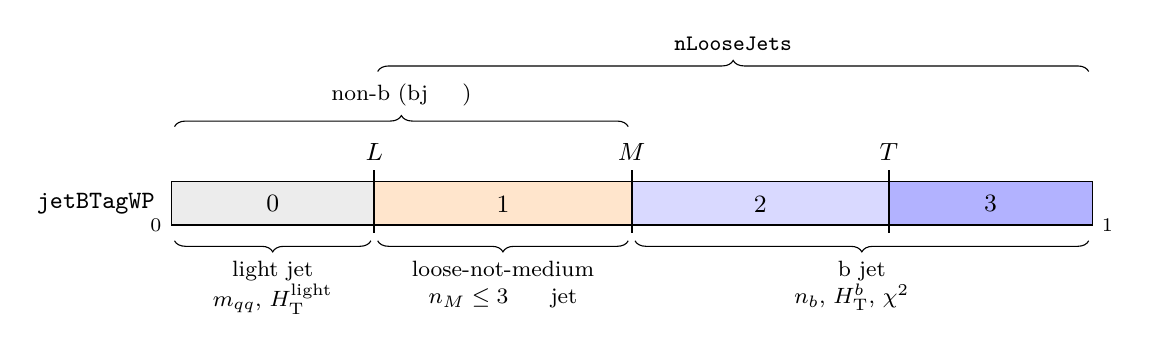
\begin{tikzpicture}[x=0.86cm,y=1cm,font=\small]
  \fill[gray!15]  (0,0) rectangle (3.0,0.55);
  \fill[orange!20](3.0,0) rectangle (6.8,0.55);
  \fill[blue!15]  (6.8,0) rectangle (10.6,0.55);
  \fill[blue!30]  (10.6,0) rectangle (13.6,0.55);
  \draw (0,0) rectangle (13.6,0.55);
  \foreach \x/\l in {3.0/L,6.8/M,10.6/T}{\draw[thick] (\x,-0.1)--(\x,0.7); \node[above] at (\x,0.7) {$\l$};}
  \node at (1.5,0.27) {0}; \node at (4.9,0.27) {1}; \node at (8.7,0.27) {2}; \node at (12.1,0.27) {3};
  \node[left] at (-0.1,0.27) {\texttt{jetBTagWP}};
  \node[left,font=\scriptsize] at (0,0) {0}; \node[right,font=\scriptsize] at (13.6,0) {1};
  \draw[decorate,decoration={brace,amplitude=4pt,mirror}] (0.05,-0.2)--(2.95,-0.2) node[midway,below=4pt,align=center,font=\footnotesize]{light jet\\$m_{qq}$, $\HT^{\text{light}}$};
  \draw[decorate,decoration={brace,amplitude=4pt,mirror}] (3.05,-0.2)--(6.75,-0.2) node[midway,below=4pt,align=center,font=\footnotesize]{loose-not-medium\\$n_M\le3$ 의 넷째 jet};
  \draw[decorate,decoration={brace,amplitude=4pt,mirror}] (6.85,-0.2)--(13.55,-0.2) node[midway,below=4pt,align=center,font=\footnotesize]{b jet\\$n_b$, $\HT^b$, \chisq{} 후보};
  \draw[decorate,decoration={brace,amplitude=4pt}] (0.05,1.25)--(6.75,1.25) node[midway,above=4pt,font=\footnotesize]{non-b (bj 쌍의 짝)};
  \draw[decorate,decoration={brace,amplitude=4pt}] (3.05,1.95)--(13.55,1.95) node[midway,above=4pt,font=\footnotesize]{\texttt{nLooseJets}};
\end{tikzpicture}
\caption{b-tag 점수의 칸(눈금은 비례하지 않음). WP 는 2017 DeepJet $L/M/T=0.0532/0.3040/0.7476$, 2024 UParTAK4 $0.0246/0.1272/0.4648$ (EraConfig::btagWP).}
\label{fig:reco-wp}
\end{figure}

% -----------------------------------------------------------------------------
\section{\texorpdfstring{$\chi^2$}{chi2} 쌍 짓기}\label{sec:reco-chi2}

\subsection{AN 의 정의}
AN 은 jet 넷을 두 쌍으로 나눠 두 boson 의 질량과 비교한다\src{AN-22-122 v26, PDF p.49, eq.\ 3--5}:
\begin{equation}
\chi^2_{XY}=\frac{(m_{j_1j_2}-m_X)^2}{\sigma_{j_1j_2}^2}+\frac{(m_{j_3j_4}-m_Y)^2}{\sigma_{j_3j_4}^2},\qquad XY\in\{HH,\,ZZ,\,ZH\}
\label{eq:reco-chi2}
\end{equation}
이고 $m_H=125\GeV$, $m_Z=91.2\GeV$ 다. $\sigma$ 는 ``JER 의 함수''라고만 적혀 있고 식이나 수치는 없다\src{AN-22-122 v26, PDF p.49, l.741--743}. jet 넷은 b-tag 다중도에 따라 고른다
\src{AN-22-122 v26, PDF p.51, l.744--751}: medium b jet 이 4 개면 그 넷, 5 개 이상이면 모든 b jet 조합에서 \chisq{} 가 가장 작은 넷, medium 3 개 +
loose 가 있으면 넷째는 loose 에서, loose 도 없으면 light jet 에서. 모든 후보와 순열을 돌아 가장 작은 \chisq{} 를 고른다. 출력은 세 \chisq{} 와
그 질량이다: $\chi^2_{HH}$ 의 $m_{H,1}, m_{H,2}$ 는 $m_H$ 에 가장 가까운/두 번째로 가까운 쌍의 질량, $\chi^2_{ZZ}$ 도 같은 방식, $\chi^2_{ZH}$ 는
H 후보와 Z 후보의 질량이다\src{AN-22-122 v26, PDF p.51, l.752--757}.

\begin{table}[htbp]\centering
\caption{\chisq{} 의 jet 넷 고르기(\texttt{TreeVars::chi2AN}). $n_M$ = 점수 $\ge M$ 인 jet 수.}\label{tab:reco-chi2sets}
\small
\begin{tabularx}{\linewidth}{@{}>{\raggedright\arraybackslash}p{1.6cm}L>{\raggedright\arraybackslash}p{2.6cm}@{}}
\toprule
$n_M$ & 후보 jet 넷 & 출처 \\
\midrule
$\ge4$ & M jet 가운데 모든 4 개 조합(\code{HiggsReconstructor} 가 안에서 $\binom{n_M}{4}\times3$ 쌍 짓기) & AN \tagan \\
3 & M 셋 + $[L,M)$ jet 하나(그런 jet 이 없으면 $<L$ jet 하나); 넷째 jet 의 모든 선택 & AN \tagan \\
2 & M 둘 + $[L,M)$ jet 둘(하나뿐이면 그것과 $<L$ 하나, 없으면 $<L$ 둘); 모든 선택 & 우리 확장 \tagours \\
$<2$ & 없음(모든 출력 $-1$) & \\
\bottomrule
\end{tabularx}
\end{table}

\subsection{우리 구현과 AN 과 다른 점}
\paragraph{$n_M=2$ 확장\,\tagours.}
AN 의 규칙은 $n_M\ge3$ 까지다. ttH(bb) FH 의 QCD 방법은 TR(2M + $\ge$2L)과 CR(3M + $\ge$1L)에서 DNN 입력을 계산해야 하므로(\ref{ch:qcd} 장),
$n_M=2$ 에서도 정의되게 넓혔다\src{STEP 27 §O.3}. 이때 넷째·셋째 jet 이 L–M 칸에서 오므로 이 변수는 b-tag 정의와 상관이 생긴다 —
QCD template 과 함께 쓰려면 TR/CR/SR 모양 검사를 통과해야 한다(\S\ref{sec:reco-anlist}).

\paragraph{\chisq{} 의 분모\,\tagopen.}
지금의 한 항은
\begin{equation}
\chi^2_{\text{항}}=\frac{(m_{ij}-m_X)^2}{\sqrt{0.2\,(p_{T,i}+p_{T,j})/2}}=\frac{(m_{ij}-m_X)^2}{\sqrt{0.1\,(p_{T,i}+p_{T,j})}}\quad(\pt\text{ 은 GeV 단위의 수})
\label{eq:reco-chi2ours}
\end{equation}
이다(코드 주석: ``20\,\% 분해능 가정'')\src{HiggsReconstructor.h}. 2026-06 의 인라인 코드와 비트 단위로 같게 옮긴 역사적 식이며\src{STEP 6},
STEP 27 도 그대로 두었다\src{TreeVars.h, chi2AN}. 분모가 질량의 제곱이 아니라 $\sqrt{\text{GeV}}$ 의 차원을 가지므로 이 값은 확률 해석이 있는
\chisq{} 가 아니고, 한 사건 안에서 쌍을 고르는 순위와 DNN 입력으로만 뜻이 있다. 쌍마다 분모가 $(\sum\pt)^{1/2}$ 로 커지므로 \pt{} 가 큰 쌍의 질량
차이를 덜 벌한다는 방향은 분해능과 맞는다.

\begin{note}[AN 의 ``JER 의 함수''를 식으로 — 우리 판단]
질량이 작은 두 jet 의 불변질량은 $m^2\simeq2p_1p_2(1-\cos\theta_{12})$ 이다. 각도 오차를 무시하고 오차 전파를 하면
\begin{equation}
\frac{\sigma_m}{m}=\frac12\sqrt{\left(\frac{\sigma_{p_1}}{p_1}\right)^2+\left(\frac{\sigma_{p_2}}{p_2}\right)^2}
\;\Longrightarrow\;
\sigma_{j_1j_2}=\frac{m_{j_1j_2}}{2}\sqrt{r_1^2+r_2^2},\qquad r_i=\frac{\sigma_{\pt}}{\pt}(p_{T,i},\eta_i,\rho)
\label{eq:reco-sigmajer}
\end{equation}
이다. $r_i$ 는 JME 의 JER payload(PtResolution)에서 jet 마다 읽을 수 있다. 이렇게 하면 식~\eqref{eq:reco-chi2} 가 차원 없는 \chisq{} 가 되고
사건 사이에서도 비교할 수 있다. AN 의 문장이 이 식을 뜻하는지는 확인 못 함; 바꿀지는 사용자 결정이다(\S\ref{sec:reco-open}).
\end{note}

\paragraph{두 재구성이 함께 있다.}
cut-flow 의 재구성(STEP 6)은 $n_b\ge4$ 에서만, 목표 질량 \code{cHiggsMass}\,=\,125.38, \code{cZMass}\,=\,91 로 돈다. 그 HH 결과는 cut-step
히스토그램(Higgs 후보 질량)에, ZH·ZZ 결과는 Tree 의 \code{chi2ZH}, \code{mZcandZH}, \code{mHcandZH}, \code{chi2ZZ}, \code{mZ1ZZ}, \code{mZ2ZZ} 에 간다.
Tree v1 의 \code{chi2Higgs}, \code{chi2HiggsZ}, \code{chi2Z} 와 질량들은 AN 의 jet 선택(표~\ref{tab:reco-chi2sets})과 AN 의 목표 질량(125, 91.2)을 쓴다
\src{STEP 27 §O.1}. $n_M\ge4$ 에서는 목표 질량만 다르고 알고리즘이 같다(단위 시험: $n_M=5$ 에서 비트 동일)\src{STEP 27}.

\begin{impl}
\begin{itemize}
\item \file{include/HiggsReconstructor.h}, \file{src/HiggsReconstructor.cc}: 쌍 cache(질량, $\sum\pt$, 쌍 \pt)를 만든 뒤 모든 4 개 조합의 세 쌍 짓기
      $(ij)(kl), (ik)(jl), (il)(jk)$ 를 한 번 돌며 HH·ZZ(대칭)와 ZH(두 방향)를 동시에 평가한다. 두 항을 double 로 더한 뒤 한 번만 float 로
      내린다 — 항마다 float 로 내렸을 때 옛 코드와 2,280 사건이 달랐던 것을 이렇게 맞췄다\src{STEP 6}. 동률은 먼저 찾은 것을 둔다.
\item \file{include/TreeVars.h} 의 \code{chi2AN}: 후보 넷을 만들고 \code{reconstruct} 를 불러 가설마다 최소를 둔다; HH·ZZ 질량은 목표에 가까운 순으로.
      조합 비용: $n_M=6$ 이면 45, $n_M=8$ 이면 210 쌍 짓기; $n_M=2$ 에서 $<L$ jet 이 많으면 $\binom{n}{2}$ 후보 — Tree 에 들어가는 사건에서만 계산한다.
\end{itemize}
\end{impl}

% -----------------------------------------------------------------------------
\section{event-shape 와 운동학 변수}\label{sec:reco-shape}

\subsection{운동량 텐서: sphericity, aplanarity, $C$, $D$}
선택 jet(또는 b jet)의 3-운동량으로
\begin{equation}
M_{ab}=\frac{\sum_i p_{i,a}\,p_{i,b}}{\sum_i|\vec p_i|^2},\qquad a,b\in\{x,y,z\},\qquad \lambda_1\ge\lambda_2\ge\lambda_3,\ \ \textstyle\sum\lambda=1
\label{eq:reco-tensor}
\end{equation}
의 고유값에서
\begin{equation}
S=\tfrac32(\lambda_2+\lambda_3),\quad S_\perp=\frac{2\lambda_2}{\lambda_1+\lambda_2},\quad A=\tfrac32\lambda_3,\quad
C=3(\lambda_1\lambda_2+\lambda_2\lambda_3+\lambda_3\lambda_1),\quad D=27\lambda_1\lambda_2\lambda_3
\label{eq:reco-shape}
\end{equation}
를 만든다\src{AN-22-122 v26, PDF p.51--52, eq.\ 6--11}. 범위는 $0\le S\le1$(back-to-back dijet 0, 등방 1), $0\le A\le\frac12$(등방 $\frac12$)다
(AN 은 위 끝을 $<$ 로 적었지만 등방 사건에서 등호가 된다). 우리 코드는 외부 라이브러리
\file{EventShape/Class}(D.\,G.\ Sheffield)를 정적 라이브러리 \file{lib/libEventShape.a} 로 묶어 쓰며, 위 식과 같다\src{STEP 5}. 대상이 둘 미만이면
텐서가 퇴화하므로 $-1$ 로 둔다. branch 는 jet 과 b jet 각각 다섯(\code{aplanarity} … \code{bjetEventD})이다.

\begin{note}[읽는 법]
QCD multijet 은 두 jet 이 마주보는 평평한(작은 $S$, $A$) 사건이 많고, 무거운 입자 넷(t, $\bar t$, H, H)이 붕괴하는 \ttHH{} 는 더 둥글다 — STEP 5 가 이
변수를 FH 에 선제 탑재한 이유다\src{STEP 5}. 두 가지 주의: (1) 이차 텐서는 한 jet 이 둘로 갈라지면 값이 바뀐다(collinear-unsafe); 같은 jet
정의를 쓰는 한 Data/MC 비교에는 문제가 없지만 jet 수와 상관이 크다. (2) 보통 transverse sphericity 는 횡운동량의 $2\times2$ 텐서로 정의하는데,
AN 식 8 과 우리 코드는 $3\times3$ 텐서의 $\lambda_1,\lambda_2$ 를 쓴다. 이 노트를 쓰며 라이브러리의 고유값(하삼각만 채운 \code{TMatrixDSym})을
numpy 의 전체 대칭 행렬과 무작위 2,000 사건에서 대조했고 차이는 $10^{-15}$ 수준이었다.
\end{note}

\subsection{centrality 와 Fox–Wolfram 모멘트}
AN 의 centrality 는 jet 과 lepton 의 $\sum\pt/\sum|\vec p|$ 이다\src{AN-22-122 v26, PDF p.52, eq.\ 12}. FH 에는 lepton 이 없으므로 jet 만 쓴다
(\code{centrality}, \code{bjetCentrality}). Fox–Wolfram 모멘트는
\begin{equation}
H_l=\sum_{i,j}\frac{|\vec p_i|\,|\vec p_j|}{s}\,P_l(\cos\Omega_{ij}),\qquad R_l=\frac{H_l}{H_0},\qquad l=0,\dots,4
\label{eq:reco-fw}
\end{equation}
이다($P_l$: Legendre 다항식, $\Omega_{ij}$: 두 jet 사이 각)\src{AN-22-122 v26, PDF p.53, eq.\ 16}. AN 은 ``같은 jet 의 조합도 포함한다''고 적었으므로
합은 $i=j$ 를 포함한다\src{AN-22-122 v26, PDF p.53, l.804--805}. $s$ 는 AN 에 정의가 없어 우리는 $e^+e^-$ 의 관례대로 $s=(\sum_iE_i)^2$ 로 두었다
\tagours\src{TreeVars.h}. 이 선택에서 $H_0=(\sum|\vec p_i|)^2/(\sum E_i)^2$ 로, jet 질량이 0 이면 1 이고 질량이 있으면 1 보다 조금 작다;
$R_l$ 은 그 정규화를 지운다. 질량 없는 두 jet 이 같은 에너지로 마주보면 짝수 $l$ 에서 1, 홀수 $l$ 에서 0 이다(단위 시험의 닫힌 꼴; 에너지가
다르면 홀수 $l$ 은 $(E_1-E_2)^2/(E_1+E_2)^2$). jet 과 b jet 각각
$H_0$–$H_4$, $R_1$–$R_4$ 를 남긴다. 대상이 둘 미만이면 $-1$.

\begin{note}[Fox–Wolfram 을 hadron 충돌에서 쓸 때]
$e^+e^-$ 의 질량중심계에서는 운동량 보존으로 $H_1=0$ 이지만, 우리는 실험실계에서 선택 jet 만으로 계산하므로 $H_1\ne0$ 이고 $z$ 방향 boost 에 따라
값이 바뀐다. AN 도 같은 정의를 썼으므로 Run 2 와의 정합을 위해 그대로 둔다(D-2026-10-10-B: 억지로 바꾸지 않는다).
\end{note}

\subsection{쌍 통계, HT, 질량}
쌍의 집합 $\mathcal P$ 를 셋 둔다: \textbf{jj}(모든 선택 jet 의 $i<j$), \textbf{bb}(b jet 의 $i<j$), \textbf{bj}(b jet 과 non-b jet 의 모든 쌍).
$\Delta R=\sqrt{\Delta\eta^2+\Delta\phi^2}$ 이고 $\Delta\phi$ 는 $[0,\pi]$ 로 접는다. 각 $\mathcal P$ 에서
\begin{equation}
\overline{\Delta R}=\frac1{|\mathcal P|}\sum_{\mathcal P}\Delta R,\quad \Delta R^{\min},\ \Delta R^{\max},\quad
\overline{\Delta\eta}=\frac1{|\mathcal P|}\sum_{\mathcal P}|\Delta\eta|,\quad \Delta\eta^{\max},\quad
m^{\Delta R^{\min}},\ \pt^{\Delta R^{\min}}
\label{eq:reco-pairs}
\end{equation}
일곱을 남긴다(마지막 둘은 $\Delta R$ 가 가장 작은 쌍의 질량과 \pt; AN Table 43 의 $\Delta R^{\min}_{jj,\text{mass}}$, $\Delta R^{\min}_{jj,\pt}$).
세 집합 $\times$ 일곱 = 21 개다. 그 밖에
\begin{itemize}
\item $\HT=\sum\pt$(선택 jet), $\HT^b$(b jet), $\HT^{\text{light}}$(점수 $<L$); 평균 질량 $m_j^{\text{avg}}, m_b^{\text{avg}}, m_{\text{light}}^{\text{avg}}$ 와
      $(m^2)_b^{\text{avg}}=\sum m_b^2/n_b$(AN 기호 그대로);
\item $m_{jjj}^{\max\pt}$: 서로 다른 세 jet 가운데 합 벡터의 \pt{} 가 가장 큰 조합의 질량; $m_{jbb}^{\max\pt}$: 서로 다른 b jet 둘과 그 둘이 아닌 jet 하나;
\item $m_{qq}$(\code{invMassHadW}, 식~\eqref{eq:selection-mqq}), \code{nLooseJets}(점수 $\ge L$, b 포함), \code{lightjetNumber}.
\end{itemize}
정의되지 않으면(대상 부족) $-1$ 이고 NaN 은 없다\src{TreeVars.h}.

\begin{andiff}[옛 helper 와 다른 점(STEP 27 이 고친 것)]
2026-06 의 \code{event} helper(\code{getStats}, \code{getStatsComb}, \code{getFoxWolfram}, \code{getMaxPTSame/Comb})는 그대로 두고 Tree 에는 쓰지 않는다.
다른 점은 모두 의도한 것이다\src{TreeVars.h}\src{STEP 27}: (1) $\Delta\phi$ 를 접지 않아 $\pm\pi$ 를 건너는 쌍의 $\Delta R$ 이 틀렸다;
(2) Fox–Wolfram 이 $i<j$ 만 더했다(AN 은 $i=j$ 포함); (3) bj 통계가 b jet 을 자기 자신과 짝지어 $\Delta R=0$ 이 생겼다; (4) $m_{jjj}$ 조합이 같은 jet 을
두 번 쓸 수 있었다; (5) $(m^2)_b^{\text{avg}}$ 를 $(\sum m)^2/n$ 으로 계산했다. 옛 FHSample(2024-06; 사용자의 FH DNN V3 학습 표본)의 해당 열도
같은 helper 로 만들어졌다\src{PLAN\_ML\_SYST §5.2}.
\end{andiff}

% -----------------------------------------------------------------------------
\section{AN 변수 목록과 Tree v1}\label{sec:reco-anlist}

DL DNN 은 Table 43 의 변수 전부와 GATJA 출력 24 개를 입력으로 쓰고\src{AN-22-122 v26, PDF p.50, Table 43}\src{AN-22-122 v26, PDF p.115},
SL DNN 은 333 개 후보에서 고른 50 개를 쓴다\src{AN-22-122 v26, PDF p.108, Table 49}. FH 에서 계산할 수 있는 Table 43 의 변수는 Tree v1 이 덮는다
(표~\ref{tab:reco-an43}).

\begin{table}[htbp]\centering
\caption{AN-22-122 Table 43 의 묶음과 Tree v1 의 대응. ``벡터''는 jet 벡터에서 내보내기 도구가 만든다.}\label{tab:reco-an43}
\small
\begin{tabularx}{\linewidth}{@{}>{\raggedright\arraybackslash}p{3.0cm}>{\raggedright\arraybackslash}p{4.6cm}L@{}}
\toprule
묶음 & AN 변수 & 우리 Tree(이름) \\
\midrule
다중도 & $N_{\text{jets}}$, $N_{\text{bjets}}$, $N_{\text{light}}$ & \code{nJets}, \code{nbJets}, \code{lightjetNumber} \\
4-운동량 & jet·b jet 1–6 의 \pt, $|\eta|$; lepton 1, 2 & 벡터(\code{jetPt}, \code{jetEta}, \code{jetPhi}, \code{jetMass}, \code{bTagScore}); lepton 은 FH 에 없음 \\
HT & $\HT$, $\HT^b$, $\HT^{\text{light}}$, $\HT^{\text{lepton}}$, $S_T$ & \code{HT}, \code{bjetHT}, \code{lightjetHT}; $\HT^{\text{lepton}}$, $S_T$ 없음 \\
질량 & $m_j^{\text{avg}}$, $m_b^{\text{avg}}$, $m_{\text{light}}^{\text{avg}}$, $(m^2)_b^{\text{avg}}$, $m_{jjj}^{\max\pt}$, $m_{jbb}^{\max\pt}$, $m_{\mu\mu}$, $m_{ee}$ & \code{jetAverageMass}, \code{bjetAverageMass}, \code{lightjetAverageMass}, \code{bjetAverageMassSqr}, \code{maxPTmassjjj}, \code{maxPTmassjbb}; $m_{\ell\ell}$ 없음 \\
각도 & $\overline{\Delta\eta}_{jj}, \overline{\Delta\eta}_{bb}, \Delta\eta_{bb}^{\max}$, $\overline{\Delta R}_{jj,bb}$, $\Delta R^{\min}_{jj,bb}$, 최소 $\Delta R$ 쌍의 질량·\pt & 21 개(jj, bb, bj $\times$ 7; 식~\eqref{eq:reco-pairs}) \\
\chisq{} & $\chi^2_{HH}$, $\chi^2_{ZZ}$, $\chi^2_{ZH}$ & \code{chi2Higgs}, \code{chi2Z}, \code{chi2HiggsZ} \\
질량·\pt{} & $m_{H,1}$, $m_{H,2}$, $m_{Z,1}$, $m_{Z,2}$, $m_{ZH,Z}$, $m_{ZH,H}$, $\pt(H_{1,2})$ & \code{invMassH1/H2}, \code{invMassZ1/Z2}, \code{invMassHiggsZ2}(Z), \code{invMassHiggsZ1}(H), \code{PTH1/PTH2} \\
event shape & aplanarity, centrality, sphericity, $S_\perp$, $C$, $D$(jet, b jet) & STEP 5 의 열, \code{centrality}, \code{bjetCentrality} \\
(표 밖) & Fox–Wolfram $H_0$–$H_4$, $R_1$–$R_4$; jet b-tag 판별값; GATJA 24 & \code{H0}…\code{bjetR4}; \code{bTagScore}(2024 는 \code{jetBTagWP}); GATJA 는 학습 뒤 \\
\bottomrule
\end{tabularx}
\end{table}

\paragraph{없는 것.}
(1) \textbf{BLR}(b-tag likelihood ratio; 6b 대 4b 가설의 b-tag pdf 비, AN eq.\ 17--19)\src{AN-22-122 v26, PDF p.55--56}: 맛별 b-tag pdf 가
필요하다 — 내보내기 도구에서 나중에(PLAN\_ML\_SYST §5.1). (2) \textbf{JABDT}: SL 의 6-jet 가설(lepton top 의 b 포함)이라 FH 에는 새 가설이 필요하다.
(3) \textbf{MEM}: ttH(bb) FH 는 MEM 판별값을 ANN 입력으로 썼지만\src{AN-19-094 v20, PDF p.113--114} ttHH AN 에는 없다. (4) \textbf{GATJA 출력}: FH 판을
학습한 뒤(W5). (5) lepton·\MET{} 변수는 FH 에 해당 없음(\code{metPhi} 는 남김). (6) GATJA 의 이웃 번호(\chisq$(m_H)$ 가 가장·두 번째로 작은 짝)는 내보내기
도구가 b jet 4-벡터로 만든다\src{PLAN\_ML\_SYST §5.1}.

\paragraph{b-tag 와 상관된 입력의 제약.}
ttH(bb) FH 는 QCD template 을 낮은 b-tag 영역에서 가져오므로 b-tag 값과 직접 상관된 입력을 피하고, TR·CR·SR 에서 모양이 같은 변수만 썼다
\src{AN-19-094 v20, PDF p.156}. ttHH SL DNN 은 b-tag 점수 순위(d3–d6)와 BLR 을 많이 쓴다\src{AN-22-122 v26, PDF p.108, Table 49}. FH 에서는 이 둘이 부딪힌다:
권고는 ``모양 동등성 검사를 통과한 변수만''이다(사용자 결정 대기)\tagopen\src{ROADMAP\_FH §6}. 2024 는 fixed-WP SF 만 있으므로 연속 점수 대신
WP 칸(\code{jetBTagWP})을 쓰는 것이 SF 와 맞다\src{D-2026-10-10-A}.

% -----------------------------------------------------------------------------
\section{jet 단위 정보와 GATJA 의 정답 표지}\label{sec:reco-gen}

\paragraph{jet 벡터.}
선택 jet 마다(\code{jetPt} 와 같은 순서, 보정 뒤 \pt{} 내림차순) \code{jetPt}, \code{jetEta}, \code{jetPhi}, \code{jetMass}, \code{bTagScore},
\code{jetBTagWP}, MC 의 \code{hadFlavs}, \code{partonFlavs} 가 있다. jet 배정 ML 의 입력(노드의 \pt, $\eta$, $\phi$, b-tag)을 모두 여기서 만들 수 있다.

\paragraph{정답 표지(MC; \texttt{include/GenMatch.h}).}
\begin{enumerate}
\item \textbf{parton}: $|\text{pdgId}|=1$–5 인 quark 가운데 statusFlags 의 fromHardProcess(bit 8)와 isLastCopy(bit 13)가 모두 켜진 것. 마지막 사본은
      parton shower 뒤 hadronization 직전이라 jet 방향에 가깝다.
\item \textbf{기원}: quark 자신의 사본을 건너뛴 첫 다른 $|\text{pdgId}|$ 조상. H(25)의 b → 1, t(6)의 b → 2, W(24) → 3, Z(23) → 4. 그 밖(4FS tt+bb 의 추가
      b, gluon 분열 등)은 parton 이 아니다.
\item \textbf{어미 번호}: 그 조상의 \emph{첫} 사본의 GenPart 번호 — 같은 Higgs 의 두 b 가 같은 번호를 가진다.
\item \textbf{짝짓기}: $\Delta R<0.4$($\Delta\phi$ 접음)인 모든 (jet, parton) 쌍을 $\Delta R$ 오름차순으로 보며 jet 과 parton 을 각각 한 번만 쓴다(greedy unique).
\end{enumerate}
결과는 \code{jetGenMatch}(0 없음, 1 H$\to$b, 2 t$\to$b, 3 W$\to$q, 4 Z$\to$q), \code{jetGenMotherIdx}(없으면 $-1$), 그리고
\code{jetGenTopIdx}(그 quark 가 온 top 의 첫 사본: t$\to$b 는 어미 자신, W$\to$q 는 W 의 첫 사본의 부모가 top 이면 그 top; 아니면 $-1$)다.
Data 는 0, $-1$, $-1$\src{GenMatch.h}\src{STEP 27 §O.2, §P}. top 번호는 독립 검토에서 더했다\tagimpl\tagtest: FH 에는 hadronic top 이 둘이라
W 의 번호만으로는 W 의 두 quark 가 어느 top 의 b 와 한 묶음인지 알 수 없고(GenPart 는 tree 에 없다), top 재구성의 정답이 없었다. AN 의 JABDT 는 jet 과 gen jet 의 $\Delta R<0.4$ 로 매칭하고 $\Delta R$ 가 가장 작은 순열을 ``맞는 것''으로 했다
\src{AN-22-122 v26, PDF p.58} — 발표는 이를 ``$\Delta R$ 합이 가장 작은 순열''로 적었다\src{사전승인 발표 p.40}\src{승인 발표 p.40}; 0.4 는 AK4 의 반지름이다. 이 규칙은 PROPOSED 이고 사용자 확인을 기다린다\tagopen.

\paragraph{GATJA 가 이것을 필요로 하는 이유.}
GATJA 는 b-tag 된 jet \emph{하나하나}를 Higgs / top / 기타로 분류하는 object 기반 배정이다\src{GATJA 발표 p.6}. 각 b jet 을 노드로 두고, 그 jet 과
짝지었을 때 $\chi^2(m_H)$ 가 가장 작은 jet 과 두 번째로 작은 jet 을 이웃으로 붙인다 — 혼잡한 말단 상태에서는 맞는 짝이 두 번째인 경우가 많기
때문이다\src{GATJA 발표 p.7}. 출력은 b jet 마다 세 확률이고 최대 8 개 b jet 이라 24 개다\src{AN-22-122 v26, PDF p.69, Table 48}. 이것은 지도 학습
(supervised)이므로 jet 마다 ``진짜 기원''이 있어야 한다: \code{jetGenMatch} 1 → Higgs, 2 → top, 그 밖 → 기타가 GATJA 의 세 class 이고, FH 에서는 W
(표지 3)를 넷째 class 로 넓힐 수 있다\src{PLAN\_ML\_SYST §9.3}. 어미 번호는 ``어느 두 jet 이 같은 Higgs 인가''를 주므로 GATJA 발표의 새 출력
(best pairing)\src{GATJA 발표 p.8} 과 \chisq{} 재구성 효율(AN Table 47 같은 표)을 재는 데 쓴다. DL 에서 GATJA 를 넣으면 $Z_A$ 가 27\,\% 좋아졌다
\src{AN-22-122 v26, PDF p.116, l.1184--1185}.

\begin{note}[표지의 한계]
두 quark 가 한 jet 에 들어가면(병합) 하나만 표지를 받는다; acceptance 밖의 quark 는 jet 이 없다; FSR 로 방향이 바뀌면 $\Delta R<0.4$ 를 놓칠 수 있다.
그래서 ``H 에 매칭된 b jet 쌍의 질량이 125\GeV{} 근처에 모이는가''로 실제 v15 표본에서 확인한다\src{STEP 27, 확인하지 못한 것}. 표지는 선택이나 weight 에
쓰지 않는다.
\end{note}

% -----------------------------------------------------------------------------
\section{계통용 weight}\label{sec:reco-weights}
Tree v1 은 MC 사건마다 계통 불확도의 재료를 남긴다(\ref{ch:syst} 장)\src{STEP 27 §O.4, §O.5}.
\begin{itemize}
\item \code{PUWeight_up/_down}: \code{CorrectionsManager::getPUWeight}. Run 2 는 LUM payload, 2024 는 우리 DQM 판 JSON(최소 편향 $\sigma\pm4.6\,\%$).
\item \code{L1PrefiringWeight_up/_down}: 2016·2017 MC 의 NanoAOD 값(그 연도에는 필수 branch), 2018·2024 는 1.
\item \code{LHEScaleWeight}, \code{PSWeight}: NanoAOD 벡터 그대로. 순서는 branch 제목이 정한다 — 보통 9 개($\mu_R,\mu_F$)와 4 개(ISR, FSR)지만 기억이므로
      실제 v15 파일의 제목으로 확인한다\tagopen.
\item \code{LHEPdfWeight}: 사건당 약 100 float 이라 \texttt{-{}-tree-pdf on} 일 때만(제출기도 같은 옵션).
\item Run 2 b-tag shape 출처 8 개 $\times$ up/down(\code{bTagWeight_hf_up} …): BTV recipe — c jet 은 cferr1/2 에서만, b·light jet 은 cferr 밖의 모든 출처에서
      변형. 출처별 norm reweight 는 reweight 도구가 유도해 downstream 이 곱한다(AN 은 ``변동마다 따로'')\src{AN-22-122 v26, PDF p.42}.
\item 2024: \code{bTagWeight_up/_down}(fixed WP), 비교 weight \code{bTagWeight_oldRule}, \code{bTagWeight_cAsB}\src{D-2026-10-10-A}.
\end{itemize}
JES·JER 변형은 weight 가 아니라 다시 실행해야 한다(W6). 출처별 shape weight 의 키(\code{up_hfstats1} 등)는 job 이 시작할 때 레시피의
flavour 마다 한 번씩 계산해 보고, payload 가 하나라도 모르면 그 자리에서 멈춘다(E40)\tagtest\src{STEP 27 §P}: 계산 실패를 SF = 1 로 바꾸는 옛 함수
때문에 변형이 조용히 틀릴 수 있었다(독립 검토 R2).

\paragraph{Tree v1 끄기\,\tagimpl\tagtest.} Tree v1 은 압축 전 tree byte 의 55–60\,\% 를 차지한다(합성 출력에서 잰 값\src{STEP 27 §P}). ML 입력이 필요
없는 실행(btagtrig, lepton CR)에서는 analyzer 와 제출기의 \texttt{-{}-tree-v1 off} 로 Tree v1 branch 를 모두 뺄 수 있다; 나머지 branch·히스토그램은
같다(offline smoke 에서 확인). \texttt{-{}-tree-pdf on} 은 Tree v1 이 켜져 있을 때만 된다.

% -----------------------------------------------------------------------------
\section{검증}\label{sec:reco-tests}
\begin{itemize}
\item \textbf{단위 시험} \file{test/test_TreeVars.cc}(30 check, 모두 PASS; STEP 27 의 27 + P 의 top 번호 3): $\Delta\phi$ 접기와 $\pm\pi$ 를 건너는 쌍, 쌍 통계와 무차별 계산, Fox–Wolfram 의 닫힌
      꼴과 무차별 이중합, centrality·HT·평균 질량, 서로 다른 세 jet 의 $m_{jjj}$, \chisq{}: $n_M=5$ 에서 \code{HiggsReconstructor} 와 비트 동일·무차별과 같음,
      질량 순서, $n_M=3$(L 있음·없음), $n_M=2$(L 하나), $n_M=1\to-1$; 정답 표지: 합성 gen record(H 의 두 b 사본, t$\to$b, W$\to$q 둘, hard process 가
      아닌 b, $\pm\pi$ 를 건너는 Z$\to$b)에서 표지·어미·유일성\src{STEP 27}. 기대값은 시험 안에서 독립적으로 계산한다.
\item \textbf{독립 재계산} \file{test/offline_smoke/treev1_check.py}: analyzer 출력 다섯(2024 MC, 2024 MC \texttt{-{}-tree-pdf on}, 2024 Data, 2017 MC,
      2017 Data)의 모든 사건에서 Tree 의 jet 벡터로 모든 Tree v1 변수를 numpy 로 다시 계산하고, 입력 파일의 같은 사건으로 \code{metPhi}, 정답 표지,
      PU up/down(correctionlib), L1 up/down, LHE/PS 벡터, 2017 의 shape 출처 16 개를 대조한다.
\item \textbf{offline smoke} 116/116(STEP 27 의 110 + P 의 6: \texttt{-{}-tree-v1 off} 와 그 금지 조합, shape 키 검사와 키가 빠진 payload), 2017 출력은 전 빌드와 같다(Y1)\src{STEP 27 §P}.
\item \textbf{병합}: 두 빌드의 출력(예: 다시 빌드한 뒤 재제출한 job)이 섞이면 hadd 가 실패하지 않고 branch 나 사건을 조용히 잃는다(독립 검토 R1).
      \file{outputMerger/run_one_hadd.sh} 가 hadd 전에 입력의 \code{Tree/Tree} branch 집합을 비교해 다르면 exit 8 로 멈춘다\tagtest\src{STEP 27 §P}.
\end{itemize}

% -----------------------------------------------------------------------------
\section{변경 이력}\label{sec:reco-history}
\begin{itemize}
\item \textbf{STEP 5} (2026-06-11): EventShape 를 소스 include 대신 \file{lib/libEventShape.a} 로; 사건 형태 10 branch\src{STEP 5}.
\item \textbf{STEP 6} (2026-06-12): \code{HiggsReconstructor} — HH 만 하던 인라인 재구성을 HH/ZH/ZZ 한 번의 sweep 으로; ZH·ZZ 6 branch;
      옛 HH 와 비트 동일(10,000 사건, 2,280 mismatch 를 고친 뒤 0)\src{STEP 6}.
\item \textbf{STEP 27} (2026-10-10): Tree v1 — branch 75 개 + 연도별 16(Run 2 shape) 또는 2(2024), \code{--tree-pdf}; \file{include/TreeVars.h},
      \file{include/GenMatch.h}; 제출기 \code{--memory} 기본 2 GB(전 12 GB 고정; 2024 analyzer job 25,313 개의 최대 286 MB), plotter \code{--tree-v1}
      \src{STEP 27}. 계획은 \file{docs/PLAN_ML_SYST.md} §5.2.
\item \textbf{STEP 27 P} (2026-10-10, 독립 검토 반영): \code{jetGenTopIdx}(core 76 개), analyzer·제출기 \code{--tree-v1 on|off}, shape 키 검사(E40),
      병합의 branch 집합 검사(exit 8), cAsB 의 큰 jet weight 수, NaN 점수의 WP 칸 0\src{STEP 27 §P}.
\end{itemize}

% -----------------------------------------------------------------------------
\section{미결 사항}\label{sec:reco-open}
\begin{openq}
\begin{enumerate}
\item \textbf{\chisq{} 의 $\sigma$}: 식~\eqref{eq:reco-chi2ours}(역사적) 대 AN 의 ``JER 의 함수''(식~\eqref{eq:reco-sigmajer} 같은 꼴, 우리 해석).
      cut-flow·SR 정의는 그대로 두고 DNN 입력의 정의만 바꿀지\src{PLAN\_ML\_SYST §8}.
\item \textbf{Tree v1 을 SF main 셋에 넣을지} — 권고는 예(아니면 ML 표본을 위해 main 을 한 번 더)\src{ROADMAP\_FH §6}.
\item 이름 규칙(DL 새 이름 + b jet 양은 \code{bjet} 접두)과 정답 규칙은 PROPOSED — 사용자 확인\src{STEP 27}.
\item \code{LHEScaleWeight}·\code{PSWeight} 의 순서를 v15 파일의 branch 제목으로 확인; Tree 크기(합성 출력에서 사건당 약 0.7\,kB, 압축 전 tree byte 의
      55–60\,\%)와 CPU 를 첫 SF main 에서 잼; \code{--memory} 2 GB 가 Tree v1 에서도 넉넉한지; lepton CR 에 Tree v1 을 켤지(\texttt{-{}-tree-v1}).
\item DNN 입력에 b-tag 점수·BLR·$n_M=2$ \chisq{} 를 쓸지 — QCD template 과의 정합(TR/CR/SR 모양 검사)\src{ROADMAP\_FH §6}.
\item GATJA 의 FH 판: class 셋(H, t, 기타) 또는 넷(+W), event 입력에서 lepton·\MET{} 를 무엇으로 바꿀지\src{PLAN\_ML\_SYST §9.3}.
\item 목표 질량이 cut-flow 재구성(125.38/91)과 Tree v1(125/91.2)에서 다르다 — 의도한 것이지만 그림을 비교할 때 혼동하지 않도록 표기할 것.
\end{enumerate}
\end{openq}

% =============================================================================
% 8 장 — QCD 다중 제트 배경의 데이터 기반 추정 (ch:qcd)
% 출처: AN-19-094 v20 §8.1(ttH(bb) FH 의 QCD 추정), §9(불확도), §10.1(입력 검증), 결과 장;
%       tempTTHH docs/PLAN_QCD_DD.md, ROADMAP_FH.md, DECISIONS.md, STEP 24·27, Hbb 회의 FH 발표
% =============================================================================
\chapter{QCD 다중 제트 배경의 데이터 기반 추정}\label{ch:qcd}

FH 채널의 지배적 배경인 QCD multijet 은 MC 로 믿을 만하게 예측할 수 없어 데이터에서 추정한다. 이 장은 먼저 왜 그런지를 우리 control plot 과
선례로 보이고, 방법의 통계적 바탕(ABCD 식 논리와 그 가정, jet 운동학 보정의 뜻, MC 차감의 오차 전파)을 정리한다. 이어 선례인 ttH(bb) FH 의
방법(AN-19-094 §8.1: b-tag 다중도 $\times$ $m_{qq}$ 의 직교 영역, loose jet 의 운동학 보정 TF$_{\text{loose}}$, fit 에서 자유로운 정규화, 사이드밴드와
MediumLoose 폐쇄 검정)을 쪽 번호와 함께 자세히 적는다. 마지막으로 ttHH FH 로 옮기는 우리 계획(\file{docs/PLAN_QCD_DD.md})을 적는다 — 이 부분은
Tree 의 재료(STEP 27)를 빼면 모두 \tagplan{} 이다. 사용자 결정에 따라 이 작업은 lepton CR 의 Data/MC 가 합리적으로 나온 뒤에 한다
\src{D-2026-10-10-B}.

% -----------------------------------------------------------------------------
\section{왜 데이터 기반인가}\label{sec:qcd-why}

\paragraph{물리.}
$\ge6$ jet 과 b-tag 2 개 이상을 요구해도 QCD 의 단면적이 워낙 커서 QCD 가 남는다. 그 b jet 은 주로 gluon 분열($g\to b\bar b$)과 c·light jet 의
mistag 에서 온다. LO 다중 jet MC 에서 높은 jet 다중도는 matrix element 와 parton shower 의 matching·tune 에, heavy flavour 함량은 gluon 분열의
모델링에, mistag 은 detector simulation 에 달려 있어 셋 다 불확실하다. ttH(bb) FH 는 QCD MC 를 초기 연구에만 썼다: 모양과 정규화가 모두
나빴고, 2017·2018 은 PS tune 차이로 jet 다중도가 틀려서 2016 의 모양으로 재가중하고 수율을 data 에 맞췄다\src{AN-19-094 v20, PDF p.68--69}.
신호 영역에서는 QCD MC 가 통계도 모자라 ANN 학습에 쓰지 않았다\src{AN-19-094 v20, PDF p.113}.

\paragraph{우리 control plot 이 보인 것.}
\begin{itemize}
\item 2017 baseline 의 Data/MC 는 $n_b$ 와 함께 커져 $n_b\ge4$ 에서 약 1.55 였고(그림 판독 근사), QCD 를 누른 +1$\mu$ 영역에서는 나아졌지만 $n_b$ 에
      따른 경향이 남았다\src{Hbb 회의 FH 발표 p.25--26, p.29}.
\item 2024 \code{HLT_PFHT1050} \& $\HT>1200\GeV$ 영역(SF 없음)은 Data/MC 1.46 이고 넘침은 중간 b-tag 점수(light·c mistag 영역)에 있으며, jet 수의
      비는 6 에서 1.38, 13 에서 약 2 다\src{STEP 24 §18}. SF 없는 2024 main 의 $n_b\ge4$ Data/MC 는 FH 2.18, $\mu$CR 1.41, $e$CR 1.19 다
(전체로는 FH 1.40, $\mu$CR 0.84, $e$CR 0.75)\src{STATUS 10-09 (3)}.
\end{itemize}
QCD 가 MC 의 78\,\% 인 영역에서\src{STEP 24 §18}\src{STATUS 10-09 (3)} 이 정도의 어긋남을 MC 의 정규화 하나로 고칠 수 없다(우리 판단: 모양이 $n_b$,
$n_{\text{jets}}$ 에 따라 달라진다).

\paragraph{MC 통계.}
HT 로 나눈 QCD 표본에서 낮은 HT bin 의 사건 weight 가 크다. 2017 의 $\sigma L/N$ 은 HT 200–300\GeV{} 가 약 $1.1\times10^3$, 300–500 이 약
$2.5\times10^2$ 이다(발표 표의 $\sigma$, $N$ 과 42.07\fbinv{} 로 계산, $\sum w_{\text{gen}}\simeq N$ 가정)\src{Hbb 회의 FH 발표 p.46, p.49}. reco HT 가 크게 올라간
낮은 HT 사건 하나가 높은 $n_b$·$n_{\text{jets}}$ 영역에 튀는 bin 을 만든다: 2024 의 $\HT>1200$ 영역에 QCD\_HT200to400 사건 셋(weight 합 4,330)이
있었다\src{STEP 24 §18}.

\paragraph{trigger 수준의 치우침(우리 판단).}
FH trigger 는 online b-tag 를 쓰므로 QCD 사건은 mistag 된 jet 으로 trigger 를 통과하는 일이 많다. 우리 trigger SF 는 single-muon 기준 영역에서
data 와 \ttbar{} MC 로 잰다\src{Hbb 회의 FH 발표 p.16} — b jet 이 진짜인 \ttbar{} 형 사건의 효율을 고치는 것이므로 QCD 의 mistag 경로에 그대로
맞는다는 보장이 없다. 데이터 기반 추정은 이것까지 흡수한다.

% -----------------------------------------------------------------------------
\section{통계적 바탕}\label{sec:qcd-stats}

\subsection{ABCD 식 논리와 그 가정}
QCD 사건을 두 변수로 나눈다: $x$ = b-tag 칸(낮음 / 높음), $y$ = $m_{qq}$(중심창 / 사이드밴드). QCD 에서 두 변수가 독립이면
($P(x,y)=P(x)P(y)$) 네 영역의 수 사이에
\begin{equation}
N_{\text{SR}}=N_{\text{CR}}\times\frac{N_{\text{VR}}}{N_{\text{ValCR}}}
\label{eq:qcd-abcd}
\end{equation}
가 성립한다(SR, CR: 중심창의 높은·낮은 b-tag; VR, ValCR: 사이드밴드의 높은·낮은 b-tag). ttH(bb) FH 의 방법은 이 식으로 \emph{정규화}를 정하지
않는다 — 정규화는 fit 이 정한다. 대신 같은 논리를 \emph{모양}에 쓴다: SR 의 판별변수 모양을 CR 에서 가져오고, 그 옮김이 맞는지를 사이드밴드의 같은 옮김
(ValCR → VR)으로 시험한다. 이 시험이 SR 에 대해 뜻이 있으려면 ``낮음 → 높음 b-tag 의 옮김''이 $m_{qq}$ 와 무관해야 한다. 그래서 $m_{qq}$ 는 b-tag 로
영역을 정의하는 데 쓰인 jet 을 빼고 계산한다(\S\ref{sec:qcd-regions}). 우리 \code{invMassHadW} 는 점수 $<L$ 인 jet 만 쓰므로, 한 사건에서 loose jet
하나가 M 으로 승격되어도 $m_{qq}$ 값이 그대로다(light jet 이 둘 이상일 때) — 독립성을 구성으로 보장하는 성질이다(우리 판단).

\subsection{jet 단위 운동학 보정이 필요한 이유}
CR(3M + $\ge$1L)의 사건이 SR(${\ge}$4M)의 사건과 다른 점은 ``넷째 jet 이 M 이 아니라 L–M 칸에 있다''는 것이다. 그런데 tag 확률은 jet 의 $\pt$,
$\eta$, 그리고 주변 b jet 과의 거리(gluon 분열의 가까운 b 쌍)에 달려 있다. 그래서 L–M jet 의 운동학 분포는 M jet 의 것과 다르고, CR 의 모양을 그대로
쓰면 SR 의 모양이 틀린다. 운동학 $k=(\pt,\eta,\Delta R_{\min})$ 에서 ``L 이상인 jet 이 M 일'' 조건부 확률을 $\varepsilon(k)$ 라 하면, M jet 과 L–M jet 의 수의 비는
\begin{equation}
\text{TF}(k)\equiv\frac{N_M(k)}{N_{L\neg M}(k)}=\frac{\varepsilon(k)}{1-\varepsilon(k)}
\label{eq:qcd-tfdef}
\end{equation}
이다. L–M jet 이 하나인 CR 사건에 $\text{TF}(k)$ 를 weight 로 주면, 그 사건이 같은 운동학으로 SR 에 있었을 확률의 비가 된다. 정규화가 fit 에서 자유이므로
TF 의 전체 크기는 상관없고 $k$ 에 따른 \emph{모양}만 중요하다. 세 변수에 대한 곱 꼴 $f(\pt)g(\eta)h(\Delta R_{\min})$ 은 세 변수의 효과가 서로 독립이라는 근사이고,
남는 상관이 계통 불확도가 된다(\S\ref{sec:qcd-tth-unc}).

\begin{note}[L–M jet 이 여럿일 때 — 우리 판단]
ttH(bb) AN 은 ``곱 $f g h$ 를 사건의 loose b jet 에 적용한다''고만 적었다\src{AN-19-094 v20, PDF p.110, l.1230}. jet 마다 독립이라고 보면, L–M jet
$n$ 개를 가진 CR 사건이 SR(M 하나 이상 승격)로 갈 확률과 CR 에 남을 확률의 비는
\begin{equation}
w=\frac{1-\prod_i(1-\varepsilon_i)}{\prod_i(1-\varepsilon_i)}=\prod_{i=1}^{n}\bigl(1+\text{TF}_i\bigr)-1
\;\xrightarrow{\;n=1\;}\;\text{TF}_1
\label{eq:qcd-multi}
\end{equation}
이다. 반면 jet 마다의 곱 $\prod_i\text{TF}_i$ 는 ``모든 L–M jet 이 승격''의 비다. 두 식은 $n$ 에 따라 다른 모양을 주므로(TF$<1$ 이면 곱은 jet 이 많은 사건을
깎고 식~\eqref{eq:qcd-multi} 는 키운다) $n_{\text{jets}}$ 분포에서 갈린다. 우리 계획은 ``곱으로 시작하고 폐쇄 검정으로 판정''\src{PLAN\_QCD\_DD §3.3}
이므로 식~\eqref{eq:qcd-multi} 도 같은 검정에 넣는 것이 좋겠다. 또 TF 는 baseline 의 jet 묶음(맛의 섞임)에서 재므로 CR 의 L–M jet 의 맛 섞임이 다르면
치우친다 — MediumLoose 폐쇄 검정이 이런 치우침을 잡는 장치다.
\end{note}

\subsection{MC 차감의 오차와 template 통계}
CR 의 QCD 는 $Q=D-M$(data 에서 \ttbar{} 등 MC 를 뺀 것)이다. MC 정규화에 상대 오차 $\delta_M$ 이 있고 MC 분율이 $f=M/D$ 이면
\begin{equation}
\frac{\delta Q}{Q}=\frac{M}{D-M}\,\delta_M=\frac{f}{1-f}\,\delta_M
\label{eq:qcd-subtr}
\end{equation}
이다. ttH(bb) FH 의 TR 처럼 QCD 가 80\,\% 를 넘으면($f<0.2$) $\delta Q/Q<0.25\,\delta_M$ 이다. 정규화가 자유이므로 이 오차는 전체 크기보다 \emph{bin 사이의
모양}(MC 모양이 bin 마다 다른 비율로 빠짐)으로 들어온다. template 의 통계는 CR data 와 MC 의 $\sum w^2$ 로 $\text{Var}(Q_b)=D_b+\sum_{\text{MC}}w^2$ 이다.
fit 은 이를 bin 별 nuisance(Barlow–Beeston 식)로 다룰 수 있지만, AN 이 data 에서 만든 template 에도 그것을 걸었는지는 적혀 있지 않다(\S\ref{sec:qcd-tth-unc}).

\subsection{자유 정규화}
fit 에서 QCD 정규화를 사전 제약 없는 rate parameter $\mu_{\text{QCD}}$ 로 두면, SR 판별변수의 QCD 가 많은 bin(낮은 점수)이 사실상 그 control 영역이
된다. 범주를 늘릴수록 범주마다의 $\mu_{\text{QCD}}$ 가 덜 고정된다 — ttH(bb) FH 에서는 9 개가 data 로 $\pm1$–3.5\,\% 로 고정되었다(\S\ref{sec:qcd-tth-fit}).

% -----------------------------------------------------------------------------
\section{선례: ttH(bb) FH 의 방법 (AN-19-094 §8.1)}\label{sec:qcd-tth}

\subsection{영역}\label{sec:qcd-regions}
ttH(bb) FH 는 표준 방법(medium 대신 loose b-tag 사건으로 control 영역을 만들어 SR 로 외삽)을 출발점으로 삼았다\src{AN-19-094 v20, PDF p.100}.
b-tag 축(DeepJet; $n_L$ 은 L 이상인 jet 수, M 포함)과 $m_{qq}$ 축의 직교 영역은 표~\ref{tab:qcd-regions} 와 그림~\ref{fig:qcd-regions} 이다
\src{AN-19-094 v20, PDF p.101, Table 63, Fig.~50}. 영역은 범주(7, 8, $\ge9$ jet)마다 따로 쓴다\src{AN-19-094 v20, PDF p.101}.

\begin{table}[htbp]\centering
\caption{ttH(bb) FH 의 직교 영역(AN-19-094 Table 63). 괄호는 9 jet 사건의 $m_{qq}$ 경계[GeV].}\label{tab:qcd-regions}
\small
\begin{tabularx}{\linewidth}{@{}>{\raggedright\arraybackslash}p{3.6cm}LL@{}}
\toprule
b-tag (DeepJet) & 중심창 $60(72)<m_{qq}<100(90)$ & 사이드밴드 $30<m_{qq}<60(72)$ 또는 $100(90)<m_{qq}<250$ \\
\midrule
$n_M=2$, $n_L\ge4$ (2M + $\ge$2L) & \textbf{TR}: ANN 의 배경 학습 표본 & ValTR: 입력 변수 검증 \\
$n_M=3$, $n_L\ge4$ (3M + $\ge$1L) & \textbf{CR}: SR 의 QCD 모양을 여기서 & ValCR: VR 모양 검증용 \\
$n_M\ge4$ & \textbf{SR}: 최종 분석 영역(fit) & VR: 추정과 data 를 비교 \\
\bottomrule
\end{tabularx}
\end{table}

\begin{figure}[htbp]\centering
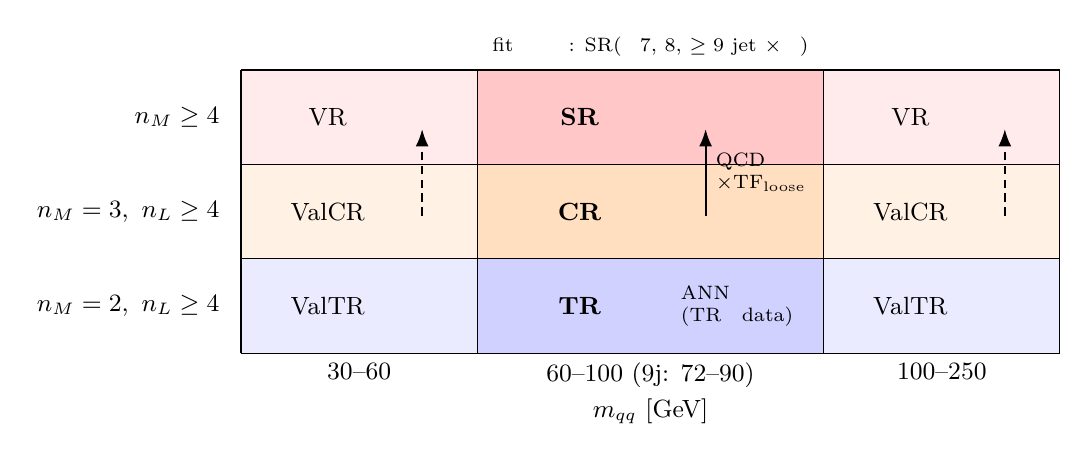
\begin{tikzpicture}[x=1cm,y=1cm,font=\small,
  cell/.style={draw,minimum height=1.15cm,align=center,inner sep=2pt},
  arr/.style={-{Latex[length=2.2mm]},thick}]
  % columns: left sideband [0,3], central [3,7.4], right sideband [7.4,10.4]
  \foreach \y/\c/\cc in {0/blue!8/blue!18, 1.2/orange!10/orange!25, 2.4/red!8/red!22}{
    \fill[\c] (0,\y) rectangle (3,\y+1.2); \fill[\cc] (3,\y) rectangle (7.4,\y+1.2); \fill[\c] (7.4,\y) rectangle (10.4,\y+1.2);}
  \draw (0,0) grid[xstep=10.4,ystep=1.2] (10.4,3.6);
  \draw (3,0)--(3,3.6); \draw (7.4,0)--(7.4,3.6);
  \node at (1.1,0.6) {ValTR}; \node at (8.5,0.6) {ValTR}; \node at (4.3,0.6) {\textbf{TR}};
  \node at (1.1,1.8) {ValCR}; \node at (8.5,1.8) {ValCR}; \node at (4.3,1.8) {\textbf{CR}};
  \node at (1.1,3.0) {VR};    \node at (8.5,3.0) {VR};    \node at (4.3,3.0) {\textbf{SR}};
  \draw[arr] (5.9,1.75)--(5.9,2.85) node[midway,right,font=\scriptsize,align=left]{QCD 모양\\$\times$TF$_{\text{loose}}$};
  \draw[arr,densely dashed] (2.3,1.75)--(2.3,2.85) node[midway,left,font=\scriptsize]{검증};
  \draw[arr,densely dashed] (9.7,1.75)--(9.7,2.85) node[midway,left,font=\scriptsize]{검증};
  \node[font=\scriptsize,align=left] at (6.3,0.6) {ANN 배경 학습\\(TR 의 data)};
  \node[anchor=east,align=right] at (-0.15,0.6) {$n_M=2,\ n_L\ge4$};
  \node[anchor=east,align=right] at (-0.15,1.8) {$n_M=3,\ n_L\ge4$};
  \node[anchor=east,align=right] at (-0.15,3.0) {$n_M\ge4$};
  \node[below] at (1.5,0) {30--60}; \node[below] at (5.2,0) {60--100 (9j: 72--90)}; \node[below] at (8.9,0) {100--250};
  \node[below] at (5.2,-0.45) {$m_{qq}$ [GeV]};
  \node[anchor=south] at (5.2,3.65) {\scriptsize fit 에 들어가는 곳: SR(범주 7, 8, $\ge9$ jet $\times$ 연도)};
\end{tikzpicture}
\caption{ttH(bb) FH 의 영역(AN-19-094 Fig.~50 을 다시 그림). 실선 화살표: CR 의 QCD 모양을 SR 로; 점선: 같은 절차를 사이드밴드에서 시험(ValCR → VR).}
\label{fig:qcd-regions}
\end{figure}

\paragraph{$m_{qq}$.}
W 질량에 가장 가까운 dijet 질량이고, 계산할 때 ``b-tag 값으로 영역을 정의하는 데 쓰인 jet'' 은 빼서 두 축이 구성상 무상관이 되게 했다
\src{AN-19-094 v20, PDF p.101, l.1171--1174}. 어떤 jet 을 빼는지(예: DeepJet 상위 몇 개)는 적혀 있지 않다(확인 못 함). baseline 에 $30<m_{qq}<250\GeV$
가 이미 들어 있다(\ref{ch:selection} 장).

\begin{openq}[AN 안의 불일치: 9 jet 의 중심창]
본문은 9 jet 의 중심창을 $70<m_{qq}<92\GeV$ 라 하고\src{AN-19-094 v20, PDF p.101, l.1162} Table 63 과 Table 65 는 $72<m_{qq}<90\GeV$ 다
\src{AN-19-094 v20, PDF p.101, p.105}. 어느 쪽이 최종인지 확인 못 함. 우리는 범주가 정해진 뒤 다시 본다\src{PLAN\_QCD\_DD §3.2}.
\end{openq}

\subsection{절차}\label{sec:qcd-tth-proc}
AN 의 네 단계\src{AN-19-094 v20, PDF p.101--103, Fig.~52}:
\begin{enumerate}
\item \textbf{CR 의 QCD}: CR 의 data 에서 \ttbar{}+jets 와 그 밖의 소수 배경(MC)을 뺀다.
\item \textbf{모양 보정}: CR 의 loose b jet 에 $\pt$, $\eta$, $\Delta R$ 기반 보정 TF$_{\text{loose}}$ 를 곱한다(\S\ref{sec:qcd-tth-tf}).
\item \textbf{SR 로}: 보정된 CR 의 QCD 모양을 SR 의 QCD 모양으로 본다. 범주마다 수율은 fit 에서 자유이고 시작값은 SR 의 (data $-$ simulation),
      simulation 은 다른 모든 배경과 신호다.
\item \textbf{검증}: 같은 1–3 을 ValCR 에 적용해 VR 의 data 와 (추정 QCD + MC) 를 비교한다.
\end{enumerate}
이를 식으로 옮기면(우리 표기; AN 에 식은 없다) 판별변수 $x$ 의 SR template 은
\begin{align}
T^{\text{SR}}_{\text{QCD}}(x)&=\mu_{\text{QCD}}\,N^{\text{SR}}_{\text{init}}\;\hat Q_{\text{CR}}(x),\qquad
N^{\text{SR}}_{\text{init}}=N^{\text{SR}}_{\text{data}}-N^{\text{SR}}_{\text{MC}},\label{eq:qcd-template}\\
\hat Q_{\text{CR}}(x)&=\frac{\sum_{e\in\text{CR,data}}w_{\text{TF}}(e)\,\delta(x-x_e)-\sum_{e\in\text{CR,MC}}w_e\,w^{t\bar t}_{\text{TF}}(e)\,\delta(x-x_e)}
{\sum_{e\in\text{CR,data}}w_{\text{TF}}(e)-\sum_{e\in\text{CR,MC}}w_e\,w^{t\bar t}_{\text{TF}}(e)}\nonumber
\end{align}
이고 $\mu_{\text{QCD}}$ 는 연도 $\times$ 범주마다 자유다.

\subsection{TF\texorpdfstring{$_{\text{loose}}$}{loose}}\label{sec:qcd-tth-tf}
M 을 통과하는 jet 은 통과하지 못하는 jet 과 $\pt$, $\eta$, $\Delta R_{\min}$(처음 두 b-tag jet 까지의 최소 거리)의 분포가 다르다 — b jet 의 운동학과 tagger
자체 때문이다. WP 가 연도마다 다르므로 연도별로 유도한다\src{AN-19-094 v20, PDF p.103, l.1215--1223}. baseline 뒤 \emph{DeepJet 값 상위 두 jet 을 뺀} jet 에서
M jet 과 L–M jet 의 수의 비를 $\pt$–$\eta$–$\Delta R_{\min}$ 공간에서 만들고, 각 축의 사영에 1 차원 함수를 차례로($\pt\to\eta\to\Delta R_{\min}$) 맞춘다
\src{AN-19-094 v20, PDF p.103--110}(AN 의 표기는 ``DeepJetM jet 대 DeepJetL jet'' 이고, 분모를 L–M 칸으로 읽은 것은 ML 검정의 같은 보정을
``L–ML 대 ML–M'' 으로 적은 서술에 맞춘 우리 해석이다\src{AN-19-094 v20, PDF p.102, l.1207--1210}). 함수는
\begin{align}
f(\pt)&=p_0+\operatorname{erf}\bigl(p_1(\pt-p_2)\bigr)\,(p_3+p_4\,\pt), \label{eq:qcd-f}\\
g(\eta)&=\sum_{i=0}^{16}p_i\,\eta^i,\qquad h(\Delta R_{\min})=\sum_{i=0}^{6}p_i\,\Delta R_{\min}^i \label{eq:qcd-gh}
\end{align}
(AN 식 13–15)이고 곱 $f(\pt)g(\eta)h(\Delta R_{\min})$ 을 사건의 loose b jet 에 적용한다\src{AN-19-094 v20, PDF p.110, eq.\ 13--15}. 보정은 data 와 \ttbar{}+jets MC 에서
따로 유도해, data 의 것은 CR 의 data 에, \ttbar{} 의 것은 CR 의 \emph{모든} MC 에 적용한다(소수 배경은 CR 에서 작고 QCD 보다 \ttbar{} 에 가깝다는 가정)
\src{AN-19-094 v20, PDF p.110, l.1235--1239}. ANN 학습 표본(TR)에도 적용한다\src{AN-19-094 v20, PDF p.113}. 보정 전후 그림은 Figs.~57–60, 2D 비는
App.\ E.1 에 있다\src{AN-19-094 v20, PDF p.108--112, p.348--353}.

\subsection{fit 에서의 QCD}\label{sec:qcd-tth-fit}
fit 에는 SR(7, 8, $\ge9$ jet $\times$ 3 년)만 들어가고, QCD 정규화는 범주마다 사전 제약 없는 nuisance
\code{CMS_ttHbb_bgnorm_ddQCD_{year}_fh_j{7,8,9}_t4} 9 개다\src{AN-19-094 v20, PDF p.235--237}. FH 단독 data fit 의 사후값은 0.912–0.974
(불확도 $\pm1.3$–3.5\,\%)이고, FH 단독 Asimov fit 의 impact 상위 10 개 가운데 9 개가 이 정규화다\src{AN-19-094 v20, PDF p.237}. 정규화는 사전 제약
없이도 SR 의 data 가 단단히 고정한다.

\subsection{검증}
\begin{itemize}
\item \textbf{$m_{qq}$ 사이드밴드(VR).} ValCR → VR 의 추정과 data 를 최종 ANN 출력에서 비교했다(전체 불확도 모델; tt+B·tt+C 는 자유 대신 50\,\% rate)
      \src{AN-19-094 v20, PDF p.104, Fig.~53}; 입력 변수는 App.\ E.2 에 있다. VR 의 QCD 는 data $-$ MC 로 맞춰져 있어 정규화는 구성상 맞고 \emph{모양만}
      검증한다 — 예: 2016 7 jet VR 은 Data 10,584, 추정 QCD 9,055, \ttbar{} 1,327, 소수 배경과 ttH 203(그림 범례)\src{AN-19-094 v20, PDF p.354--371}.
\item \textbf{MediumLoose(ML) 폐쇄 검정.} 낮은 b-tag 영역($n_M=3$, $n_L\ge4$) 안을 새 WP 로 다시 나눈다. ML WP 는 이 영역을 \ttbar{}+jets 포괄 MC 에서 둘로
      똑같이 나누는 값으로 2016 0.11185, 2017 0.101, 2018 0.093 이다\src{AN-19-094 v20, PDF p.102--103, Table 64}. CRx($n_{ML}=3$) → SRx($n_{ML}\ge4$)(사이드밴드는
      ValCRx → VRx)로 ``낮은 칸에서 높은 칸으로의 외삽''을 SR 외삽의 대리로 시험하고, 이를 위해 TF$_{\text{loose}}$ 와 같은 방식의 보정(L–ML jet 대 ML–M jet)을
      따로 유도했다\src{AN-19-094 v20, PDF p.102, l.1201--1210; p.105, Table 65}. VRx 와 SRx 두 영역에서 data 와 (추정 + MC) 의 일치가 비슷하다는 데서
      ``SR 에서도 유효한 모양''이라 결론지었다(불확도 띠는 통계만)\src{AN-19-094 v20, PDF p.103, l.1211--1214}\src{AN-19-094 v20, PDF p.106--107, Figs.~55--56}.
\item \textbf{SR 그림}은 blind: ``Data'' 는 MC 합 + CR 의 QCD 추정의 의사 data 다\src{AN-19-094 v20, PDF p.105, Fig.~54}.
\end{itemize}

\subsection{불확도}\label{sec:qcd-tth-unc}
\begin{table}[htbp]\centering
\caption{ttH(bb) FH 에서 QCD 추정에 걸린 불확도(AN-19-094 Table 79 와 본문).}\label{tab:qcd-tth-unc}
\small
\begin{tabularx}{\linewidth}{@{}>{\raggedright\arraybackslash}p{3.6cm}>{\raggedright\arraybackslash}p{3.0cm}L@{}}
\toprule
항목 & 종류 & 내용 \\
\midrule
QCD 정규화 & rate, 자유 & 연도 $\times$ 범주 9 개; 사후 $\pm1$–3.5\,\% \\
TF$_{\text{loose}}$ 보정 & shape, 단측 & up = 보정된 분포에 둘째 $\eta$ 보정 $g_2(\eta)=\sum_{i=0}^{4}p_i\eta^i$(AN 식 16)를 한 번 더 적용, down = nominal; 연도 간 비상관
      (\code{CMS_ttHbb_FH_TFLoose_{year}}); 크기 수치는 AN 에 없음 \\
template 통계 & — & data template 에 autoMCStats 를 걸었는지 명시 없음(확인 못 함) \\
비폐쇄(non-closure) & — & 별도 항목 없음(VR·ML 검증으로 정당화) \\
차감한 MC 의 불확도 & — & 전파 여부 명시 없음(확인 못 함) \\
\bottomrule
\end{tabularx}
\end{table}
단측 계통의 근거: 완벽한 보정은 변수마다의 보정을 수렴할 때까지 되풀이해야 하지만 한 번으로 끊었으므로, 그 다음 $\eta$ 재보정을 up 으로 둔다($\eta$ 와
$\Delta R_{\min}$ 사이의 약한 의존)\src{AN-19-094 v20, PDF p.110, l.1230--1234}\src{AN-19-094 v20, PDF p.154, l.1978--1985}. 표의 출처\src{AN-19-094 v20, PDF p.147, Table 79}.

\subsection{판별변수와 결과}
FH 의 판별변수는 범주마다 ttH 대 QCD 의 이진 ANN 이고, QCD 쪽 학습 표본은 TR 의 data(TF 적용; TR 은 80\,\% 넘게 QCD)다\src{AN-19-094 v20, PDF p.113}.
입력은 b-tag 값과 직접 상관된 것을 피했고\src{AN-19-094 v20, PDF p.114}, TR·CR·SR 에서 모양이 같아야 한다는 검사를 $m_{qq}$ 중심창과 사이드밴드 모두에서
통과한 변수만 썼다(예: 평균 b-tag 값은 TR 이 b-tag 로 정의되므로 탈락)\src{AN-19-094 v20, PDF p.156}. FH 단독 결과는 기대 $\mu=1.00^{+0.77}_{-0.78}$(1.3$\sigma$),
관측 $\mu=-1.31^{+0.82}_{-0.89}$ 이고 FH 단독 fit 에서는 tt+B·tt+C 정규화를 50\,\% lnN 으로 묶었다(FH 의 민감도가 약해서)\src{AN-19-094 v20, PDF p.243}.

\begin{andiff}[ttHH AN 과 다른 점]
ttHH AN(SL/DL)에는 QCD multijet 추정이 없다. DL 의 $\MET>40\GeV$ 가 QCD 억제 목적이라는 언급뿐이다\src{AN-22-122 v26, PDF p.42}. 그래서 FH 의 QCD 방법은
ttHH AN 이 아니라 ttH(bb) FH 를 선례로 쓴다\src{ROADMAP\_FH §1}.
\end{andiff}

% -----------------------------------------------------------------------------
\section{ttHH FH 로 옮기기 — 우리 계획}\label{sec:qcd-plan}
아래는 \file{docs/PLAN_QCD_DD.md}(PROPOSED, 2026-10-10)의 내용이다. 따로 표시한 것 말고는 모두 \tagplan{} 이다.

\subsection{선행 조건과 순서}
\begin{enumerate}
\item \textbf{선행(사용자)}: trigger SF 와 b-tag SF 를 켠 2024 $\mu$CR·$e$CR 의 Data/MC 가 합리적일 것 — CR·SR 에서 data 에서 빼는 것이 그 MC 이기 때문이다.
      지금은 SF 를 켠 CR 이 없고 W$\to\ell\nu$·DY 표본도 없다(D13)\src{PLAN\_QCD\_DD 결론 2}\src{D-2026-10-10-B}.
\item \code{tools/qcd/region_yields.py}(새): Tree 에서 ($n_M$, \code{nLooseJets}, \code{invMassHadW} 중심창/사이드밴드, jet 범주)별 Data·MC(과정별) 수율과
      $\sum w^2$ — TR/CR/SR/ValTR/ValCR/VR 표, QCD 비율(MC 참고), light jet 이 둘 미만인 사건의 비율.
\item \code{tools/qcd/derive_tf_loose.py}(새): baseline jet(상위 두 b-tag jet 제외)의 M/(L$-$M) 비를 $\pt$, $\eta$, $\Delta R_{\min}$ 에 차례로 맞춤; data·\ttbar{} MC
      따로, 연도별 → correctionlib JSON.
\item template 도구: CR(data $\times$ TF $-$ MC $\times$ TF$_{t\bar t}$) → SR 모양; VR 비교 그림; ML 폐쇄 검정.
\item datacard 의 QCD 과정(자유 rateParam, TF 계통, 비폐쇄 shape)\src{PLAN\_QCD\_DD §4}.
\end{enumerate}

\subsection{영역}
\ttHH{} 신호는 b quark 가 6 개라 SR 의 b 다중도가 높아질 수 있다. 그래서 SR 최적화(W5)가 어떤 $N$ 을 고르든 받아들이도록 영역을 일반화한다
\src{PLAN\_QCD\_DD §3.1}:
\begin{equation}
\text{SR}:\ n_M\ge N,\qquad \text{CR}:\ n_M=N-1,\ n_L\ge N,\qquad \text{TR}:\ n_M=N-2,\ n_L\ge N
\label{eq:qcd-general}
\end{equation}
이고 $N=4$ 가 ttH 와 같은 기준선이다.
jet 범주는 ttH 에서 $\ge9$ jet 이 가장 민감했으므로(Run 2 의 S/$\sqrt{B}$: 7j 1.47, $\ge9$j 2.14)\src{AN-19-094 v20, PDF p.587} parton 이 10 개인 \ttHH{} 는
$\ge9$, $\ge10$ jet 쪽으로 — 그 범주의 TR·CR 통계를 먼저 본다. $m_{qq}$ 는 \code{invMassHadW} 를 쓰고(점수 $<L$ 인 jet 둘 이상에서; 아니면 모든 jet) 중심창
60–100\GeV{} 로 시작한다\src{PLAN\_QCD\_DD §3.2}.

\subsection{TF, template, 2024 의 b-tag}
TF$_{\text{loose}}$ 는 연도별로 유도한다(Run 2 는 DeepJet, 2024 는 UParTAK4 의 L·M). 여러 L–M jet 의 결합(AN 에 없음)은 jet 마다의 곱으로 시작하고 ML
폐쇄 검정으로 판정한다(위 note 의 식~\eqref{eq:qcd-multi} 도 후보). template 은 CR 의 (data $\times$ TF) $-$ (MC $\times$ TF$_{t\bar t}$) 의 모양이고 정규화는
자유다. 신호를 뺄지(AN 에 없음)는 신호 오염을 재서 정한다(\ttHH{} 는 작을 것). 2024 의 CR·SR MC 는 fixed-WP b-tag weight 를 쓰므로(D-2026-10-08-A,
D-2026-10-10-A) TR·CR 의 MC 효율 map 이 그 영역에 맞는지(true-b closure, STEP 27 N)가 차감의 질을 정한다\src{PLAN\_QCD\_DD §3.3}.

\subsection{검증과 불확도}
\begin{itemize}
\item VR($m_{qq}$ 사이드밴드)과 ML 폐쇄 검정을 그대로. Run 3 tagger 에도 $[L,M)$ 를 \ttbar{} MC 에서 둘로 나누는 ML WP 를 새로 정한다.
\item \textbf{비폐쇄를 shape 불확도로 넣는 것을 권고}(ttH 는 넣지 않음): b 다중도가 높을수록 외삽이 길어 리뷰에서 물을 것이다.
\item TF$_{\text{loose}}$ 의 단측 계통(둘째 $\eta$ 보정), 차감한 MC 의 불확도 전파(AN 에 없음 → MC 변형으로 template 을 다시 만들어 전파), template 통계(CR data;
      autoMCStats 가 data template 을 덮는지 확인)\src{PLAN\_QCD\_DD §3.4}.
\end{itemize}

\subsection{DNN 의 QCD class}
ttH(bb) FH 처럼 TR 의 data(TF 적용)를 QCD class 로 쓴다(QCD MC 는 SR 통계와 모델링이 나쁘다). AN-22-122 의 다중 분류 구조(SL 9 node)에 QCD node 를 더하는
형태이고, 입력은 TR·CR·SR 모양 동등성 검사를 통과한 것만이다\src{PLAN\_QCD\_DD §3.5}\src{PLAN\_ML\_SYST §9.2}(\ref{ch:mva} 장). QCD node 로 분류된 사건은
QCD 가 많은 범주로 fit 에 들어가 QCD 정규화를 잡는 데 쓰인다.

\subsection{이미 있는 것\,\tagimpl}
STEP 27 의 Tree v1 에 영역 정의와 TF 유도에 필요한 것이 다 있다: \code{invMassHadW}($m_{qq}$), \code{nLooseJets}, jet 마다의 \code{jetBTagWP}·\code{jetPt}·\code{jetEta}·\code{jetPhi}·
\code{bTagScore}, \code{nbJets}, 그리고 $n_M=2$ 에서도 정의되는 \chisq{} 변수(\ref{ch:reco} 장)\src{STEP 27}\src{PLAN\_QCD\_DD 결론 4}. 다음은 영역별 수율 표 도구와
TF 유도 도구다(ROADMAP W7).

\begin{note}[ttHH 에서 특히 위험한 것]
\begin{itemize}
\item \textbf{외삽 길이}: SR 이 $\ge5$M 이면 CR(4M + $\ge$1L 또는 3M + $\ge$2L)에서 승격되는 jet 이 많아지고 TF 의 곱과 2 차 효과가 쌓인다 — 승격 jet 수별 폐쇄 검정.
\item \textbf{SR 통계}: 자유 정규화가 data 로 덜 고정된다 — 정규화 파라미터의 공유(연도·범주)나 CR 동시 fit 을 검토.
\item \textbf{tt+bb}: FH 단독은 tt+B 정규화에 약하다(ttH: 50\,\% lnN) — SL/DL 결합 또는 외부 제약.
\item \textbf{data 만의 결함을 template 이 흡수}: ttH(bb) FH 에서는 MEM 계산 버그가 data 에만 영향을 줬는데 data 기반 추정이 그것을 가려 보이지 않았다
      \src{AN-19-094 v20, PDF p.67} — 입력 변수의 MC–data 를 따로 점검한다\src{PLAN\_QCD\_DD §5}.
\end{itemize}
\end{note}

% -----------------------------------------------------------------------------
\section{미결 사항}\label{sec:qcd-open}
\begin{openq}
\begin{enumerate}
\item \textbf{시작 시점}: lepton CR(SF 적용)의 Data/MC 판정 — 사용자\src{D-2026-10-10-B}. W$\to\ell\nu$·DY 표본(D13)과 lepton SF(N4) 없이 판정할지.
\item \textbf{$N$ 과 jet 범주}: SR 최적화(W5)와 함께. TR·CR 의 통계를 영역 수율 표로 먼저 본다.
\item \textbf{여러 L–M jet 의 TF 결합}: 곱 대 식~\eqref{eq:qcd-multi}(우리 판단) — ML 폐쇄 검정과 $n_{\text{jets}}$ 분포로 판정.
\item \textbf{$m_{qq}$ 의 대체 규칙}: light jet 이 둘 미만인 사건은 독립성이 깨진다 — 비율을 센 뒤 그 사건을 빼거나 다른 규칙으로.
\item \textbf{신호 차감}과 \textbf{비폐쇄 불확도}(권고: 넣음)의 결정; 차감 MC 의 불확도 전파 방식.
\item \textbf{정규화의 시작값과 blinding}: AN 은 SR 의 (data $-$ MC) 를 시작값으로 썼다. 우리 blinding(D-2026-10-02-E: 최종 판별변수의 민감 bin 만 가림)과 맞추려면
      시작값을 무엇으로 할지(우리 판단: 민감하지 않은 bin 의 수율 또는 Asimov).
\item AN-19-094 에서 확인하지 못한 것: 9 jet 의 중심창(70–92 대 72–90), $m_{qq}$ 에서 빼는 jet, CR 차감에 신호를 넣었는지, TF 계통의 크기, template 통계의 처리.
\item DNN 입력: b-tag 점수·BLR·$n_M=2$ \chisq{} 를 쓰려면 TR/CR/SR 모양 동등성을 통과해야 한다(\ref{ch:reco} 장)\src{ROADMAP\_FH §6}.
\end{enumerate}
\end{openq}

% =============================================================================
% 9 장 — 다변량 분석(DNN·GATJA)
% 작성 2026-10-10 (AN_KR v0.1). 근거: AN-2022/122 v26 §6.2, §7, App. E; AN-19-094 v20 §4.8, §8.1.3, §10.1;
% GATJA 발표(2025-12-10); docs/PLAN_ML_SYST.md §2·§5·§8–§10; DECISIONS D-2026-10-10-A/B; STEP 27.
% =============================================================================
\chapter{다변량 분석(DNN·GATJA)}\label{ch:mva}

이 장은 신호와 배경을 가르는 기계학습(ML) 단계를 다룬다. 먼저 이 노트를 읽는 데 필요한 만큼의 ML 기초
— 순방향 신경망, softmax 와 cross-entropy, 최적화와 과적합, 그래프 신경망의 attention — 를 정리한다.
이어서 Run 2 ttHH AN(AN-2022/122)의 SL·DL 다중 분류 DNN 과 jet 배정 알고리즘(JABDT, GATJA)을 숫자와 함께 옮기고,
ttH(bb) FH(AN-19-094)가 QCD 를 data 에서 추정하기 때문에 b-tag 값을 입력에서 뺀 이진 ANN 을 쓴 이유를 본다.
마지막으로 우리 FH 설계(QCD class 를 더한 다중 분류 DNN, GATJA 의 FH 판), 학습 데이터와 환경, 검증 계획, 미결 사항을 적는다.
우리 쪽은 대부분 \tagplan 이다: 코드로 있는 것은 학습 입력을 담는 Tree v1(STEP 27, \tagimpl\tagtest)뿐이다.

% -----------------------------------------------------------------------------
\section{왜 다변량 분석인가}\label{sec:mva-why}

2017 FH baseline(≥6 jet, $\HT>500\GeV$, $n_b\ge2$ 등, \ref{ch:selection}장)에서 MC 합은 $3.39\times10^{6}$ event, ttHH 는 4.3 event 였다
\src{Hbb 회의 FH 발표 p.25}. 신호 대 배경 비가 $10^{-6}$ 대인 상황에서 cut 하나하나로는 신호를 살릴 수 없다.
신호의 정보는 b jet 수, 두 Higgs 후보의 질량, jet 사이 각도, event 의 모양 같은 여러 변수에 조금씩 흩어져 있고,
그 변수들은 서로 상관되어 있다. 다변량 분석은 이 정보를 한 숫자(또는 class 별 확률)로 모은다.

\begin{note}[가장 좋은 판별 변수 — Neyman–Pearson]
두 가설 S(신호)와 B(배경)를 관측량 벡터 $\vec{x}$ 로 가를 때, 주어진 배경 효율에서 신호 효율이 가장 높은 검정은
우도비 $\Lambda(\vec{x})=p(\vec{x}\,|\,S)/p(\vec{x}\,|\,B)$ 에 cut 을 거는 것이다(Neyman–Pearson 정리).
$p(\vec{x}|\cdot)$ 는 수십 차원이라 직접 만들 수 없다. 분류기(classifier)는 MC 표본에서 이 비의 단조 함수를 근사한다:
\S\ref{sec:mva-basics-ce} 에서 보듯 잘 학습된 분류기의 출력 $q_S(\vec{x})$ 는 $p(S|\vec{x})$ 에 가깝고,
$q_S/(1-q_S)\propto\Lambda(\vec{x})$ 이다. 그래서 분류기 출력 분포를 fit 하면 이 정보를 거의 다 쓸 수 있다.
\end{note}

AN-2022/122 의 두 채널은 모두 다중 분류(multi-class) DNN 으로 event 를 과정별 node 에 나누고, 각 node 의 출력 분포를
binned fit 의 판별 변수로 쓴다\src{AN-22-122 v26, PDF p.106}. 우리 FH 도 같은 전략을 따른다\src{Hbb 회의 FH 발표 p.9}\src{D-2026-10-10-B}.
그림~\ref{fig:mva-flow} 는 우리 계획의 흐름이다.

\begin{figure}[htbp]
\centering
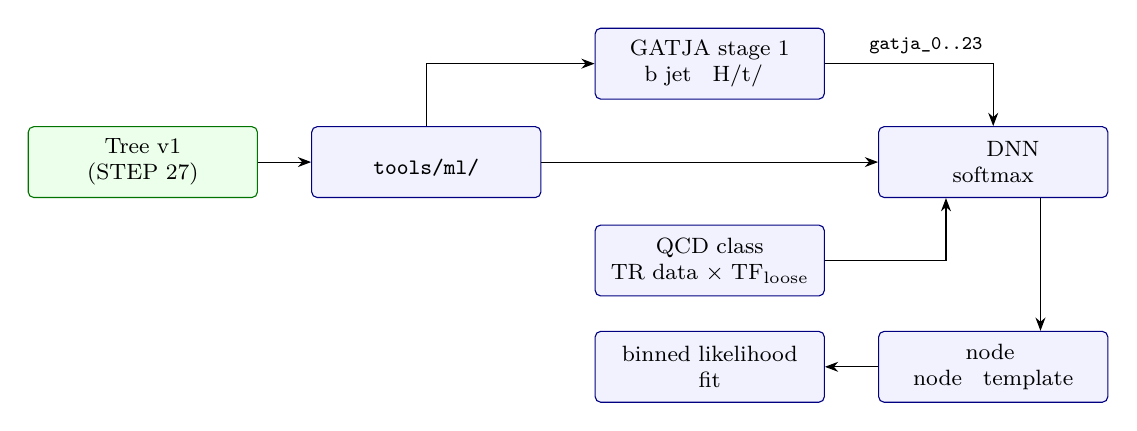
\begin{tikzpicture}[font=\footnotesize, >=Stealth,
  box/.style={draw, rounded corners=2pt, align=center, inner sep=3pt, text width=27mm, minimum height=9mm},
  done/.style={box, fill=green!8, draw=green!45!black},
  plan/.style={box, fill=blue!5, draw=blue!50!black}]
\node[done] (tree) at (0,0)      {Tree v1\\ (STEP 27)};
\node[plan] (exp)  at (3.6,0)    {내보내기 도구\\ \texttt{tools/ml/}};
\node[plan] (gat)  at (7.2,1.25) {GATJA stage 1\\ b jet 별 H/t/기타};
\node[plan] (qcd)  at (7.2,-1.25){QCD class\\ TR data $\times$ TF\textsubscript{loose}};
\node[plan] (dnn)  at (10.8,0)   {다중 분류 DNN\\ softmax};
\node[plan] (tmpl) at (10.8,-2.6){최대 node 범주화\\ node 별 template};
\node[plan] (fit)  at (7.2,-2.6) {binned likelihood\\ fit};
\draw[->] (tree) -- (exp);
\draw[->] (exp.east) -- (dnn.west);
\draw[->] (exp.north) |- (gat.west);
\draw[->] (gat.east) -| node[above, pos=0.3, font=\scriptsize]{\texttt{gatja\_0..23}} (dnn.north);
\draw[->] (qcd.east) -| ([xshift=-6mm]dnn.south);
\draw[->] ([xshift=6mm]dnn.south) -- ([xshift=6mm]tmpl.north);
\draw[->] (tmpl) -- (fit);
\end{tikzpicture}
\caption{우리 FH 의 ML 흐름(계획). 초록 = 구현·시험됨, 파랑 = 계획. QCD class 는 \ref{ch:qcd}장, fit 은 \ref{ch:stats}장. GATJA 를 넣기 전에 GATJA 없는 DNN 기준선을 먼저 만든다(PLAN\_ML\_SYST §7 B, C).}
\label{fig:mva-flow}
\end{figure}

% -----------------------------------------------------------------------------
\section{기계학습 기초 — 이 장을 읽는 데 필요한 만큼}\label{sec:mva-basics}

\subsection{순방향 신경망}\label{sec:mva-basics-ffnn}

순방향(feed-forward, fully connected) 신경망은 입력 벡터 $\vec{x}$ 에 층(layer)을 차례로 적용한다:
\begin{equation}
  \vec{h}^{(0)}=\vec{x},\qquad
  \vec{h}^{(l)}=\phi\!\left(W^{(l)}\vec{h}^{(l-1)}+\vec{b}^{(l)}\right),\quad l=1,\dots,L,
  \label{eq:mva-ffnn}
\end{equation}
여기서 $W^{(l)}$(weight 행렬)과 $\vec{b}^{(l)}$(bias)가 학습되는 parameter, $\phi$ 는 비선형 활성 함수다.
AN 은 숨은 층에 ReLU, $\phi(z)=\max(0,z)$ 를 쓴다\src{AN-22-122 v26, PDF p.109, Table 50}. "[512, 256, 128, 64]" 는 숨은 층 네 개의
node 수다. 입력 50 개, 출력 9 개이면 parameter 는 약 $2.0\times10^{5}$ 개다(우리 계산: $\sum_l (n_{l-1}+1)\,n_l$).
parameter 가 많을수록 학습 표본의 우연한 요동까지 외우기 쉽다(\S\ref{sec:mva-basics-overfit}).

\subsection{다중 분류: softmax 와 cross-entropy}\label{sec:mva-basics-ce}

마지막 층은 class 수 $K$ 만큼의 실수 $z_k$ 를 내고, softmax 가 이를 합이 1 인 확률로 바꾼다:
\begin{equation}
  q_k(\vec{x})=\frac{e^{z_k}}{\sum_{j=1}^{K}e^{z_j}},\qquad
  \mathcal{L}_{\mathrm{CE}}=-\frac{1}{\sum_n w_n}\sum_{n} w_n\sum_{k=1}^{K} y_{nk}\ln q_k(\vec{x}_n),
  \label{eq:mva-softmax-ce}
\end{equation}
$y_{nk}$ 는 event $n$ 의 정답 class 면 1, 아니면 0 (one-hot), $w_n$ 은 event 의 학습 weight 다. 이것이 categorical cross-entropy 이고,
$K=2$ 에 sigmoid 를 쓰면 binary cross-entropy 가 된다(ttH(bb) FH 의 ANN, \S\ref{sec:mva-tth}).

\begin{note}[왜 출력이 확률처럼 행동하나]
표본이 무한히 크면 손실의 기댓값은 $-\int d\vec{x}\,p(\vec{x})\sum_k p(k|\vec{x})\ln q_k(\vec{x})$ 이다. 각 $\vec{x}$ 에서 $\sum_k q_k=1$
조건으로 이를 최소화하면(Lagrange 승수) $q_k(\vec{x})=p(k|\vec{x})$ 가 나온다. 즉 출력은 \textbf{학습 표본의 class 구성비}를 사전 확률로 한
사후 확률이다. class weight $c_k$ 를 곱하면 $q_k\propto c_k\,p(k|\vec{x})$ 가 되어 경계가 움직인다. fit 은 출력의 "확률 값"이 아니라
모양(template)만 쓰므로 이것은 틀린 것이 아니다 — 같은 네트워크를 MC 와 data 에 똑같이 적용하기만 하면 된다.
\end{note}

event 는 출력이 가장 큰 node 로 보낸다(최대 node 범주화). 그러면 한 event 가 한 범주에만 들어가 범주들이 통계적으로 독립이다
\src{사전승인 발표 p.18}\src{AN-22-122 v26, PDF p.112}.

\textbf{class weight 와 event weight}.\label{sec:mva-basics-weights} 식~\eqref{eq:mva-softmax-ce} 의 $w_n$ 에는 두 가지가 섞인다. (1) event weight($\sigma\mathcal{L}/\sum w_{\mathrm{gen}}\times$SF)는 한 class 안에서
하위 과정의 비(tt 의 SL·DL·FH 붕괴, stitching 된 tt+HF 범주)를 맞춘다. (2) class weight(흔히 $c_k=N_{\mathrm{tot}}/(K N_k)$)는 작은 class 가
손실에서 묻히지 않게 한다. AN 은 "different training weight" 로 최적화했다고만 쓰고 값은 없다\src{AN-22-122 v26, PDF p.107}. SWAN 의 우리 FH
시험 판(V3)은 event weight 없이 표본을 일정 비율로 덜어낸 뒤 균형식 class weight 를 썼다\src{PLAN\_ML\_SYST §2.4}. NLO 표본의 음의 weight 처리도
정해야 한다(우리 판단).

\subsection{최적화: Adam, LAMB, 학습률 감쇠}\label{sec:mva-basics-opt}

parameter $\theta$ 는 손실의 기울기 $g_t=\nabla_\theta\mathcal{L}$ 를 mini-batch(AN: 1024 event)마다 계산해 갱신한다. Adam 은 기울기의 1·2차
이동 평균으로 parameter 마다 보폭을 조절한다:
\begin{equation}
  m_t=\beta_1 m_{t-1}+(1-\beta_1)g_t,\quad v_t=\beta_2 v_{t-1}+(1-\beta_2)g_t^2,\quad
  \theta_t=\theta_{t-1}-\eta_t\,\frac{\hat m_t}{\sqrt{\hat v_t}+\epsilon},
  \label{eq:mva-adam}
\end{equation}
($\hat m_t, \hat v_t$ 는 초기 편향을 보정한 값). LAMB 는 Adam 의 갱신량을 층마다 $\|\theta^{(l)}\|/\|r_t^{(l)}\|$ 로 다시 재어(trust ratio)
큰 batch 에서도 층마다 같은 비율로 움직이게 한다. AN 의 DL DNN 이 LAMB 를 쓰고\src{AN-22-122 v26, PDF p.116--117, Table 51}, GATJA 도 "큰 batch
optimizer" 를 쓴다(공개 코드는 LAMB)\src{GATJA 발표 p.10}\src{PLAN\_ML\_SYST §2.2}.
학습률 $\eta_t$ 는 처음에 크게(빠른 탐색), 나중에 작게(안정) 둔다. AN SL 은 지수 감쇠
\begin{equation}
  \eta(\text{epoch})=\eta_0\times0.99312^{\,\text{epoch}},\qquad \eta_0=2\times10^{-5}
  \label{eq:mva-lrdecay}
\end{equation}
를 쓴다\src{AN-22-122 v26, PDF p.109, Eq.~20, Table 50}. $0.99312^{100}\approx0.50$ 이므로 학습률은 100 epoch 마다 절반이 된다(우리 계산).
$\eta_0$ 는 $10^{-3}, 10^{-4}, 5\times10^{-5}, 2\times10^{-5}, 10^{-5}$ 가운데 손실 분포가 가장 좋은 것으로 골랐다\src{AN-22-122 v26, PDF p.108}.
DL 은 cosine 감쇠, $\eta_t=\eta_{\min}+\tfrac12(\eta_0-\eta_{\min})\bigl(1+\cos(\pi t/T)\bigr)$ 를 쓴다\src{AN-22-122 v26, PDF p.117, Table 51}.

\subsection{과적합, 검증, 홀짝 분할}\label{sec:mva-basics-overfit}

과적합(overtraining)은 네트워크가 학습 표본의 우연한 요동을 외워 새 표본에서 성능이 떨어지는 상태다. 대책은 셋이다.
(1) 정규화: dropout(학습 때 node 일부를 무작위로 끔; AN 0.2), L2 weight decay. (2) 조기 종료: 학습에 쓰지 않은 validation 표본의 손실을
본다. AN SL 은 학습·검증 손실 차가 1 \% 를 넘으면 멈추되 최소 100 epoch 은 돌리고\src{AN-22-122 v26, PDF p.107; p.109, Table 50}, 그 가운데
$Z_A$(식~\eqref{eq:mva-za})가 가장 큰 epoch 을 고른다. (3) 독립 평가: AN 은 MC 의 홀수 event number 로 학습하고(그 안을 학습 55 \%, 검증 25 \%,
test 20 \%로) 짝수 event 로 template 을 만든다\src{AN-22-122 v26, PDF p.106, 109}. 이것은 $k=2$ k-fold 의 한 방향이다 — 두 방향(홀→짝,
짝→홀)을 다 쓰면 MC 전부가 template 에 들어간다. 과적합은 학습·test 표본의 출력 분포를 겹쳐 Kolmogorov–Smirnov(KS) 검정으로 본다.
AN 은 node 별 train/test 비교를 부록 E 에 둔다\src{AN-22-122 v26, PDF p.211--214, Fig.~E.1--E.4}.

\subsection{입력 전처리}\label{sec:mva-basics-prep}

변수마다 크기와 꼬리가 다르면(\HT 는 수백--수천 GeV, $\dR$ 는 0--5) 학습이 불안정하다. 흔한 변환은 표준화 $\hat x=(x-\mu)/\sigma$
(ttH(bb) FH\src{AN-19-094 v20, PDF p.114}), 분위수 변환(QuantileTransformer, [0,1] 균등 분포로) 뒤 MinMaxScaler(AN\src{AN-22-122 v26, PDF p.107--108}),
RobustScaler(SWAN V3)다. 분위수 변환은 긴 꼬리와 이상값에 강하다. 변환은 학습 표본에서 한 번 정해 평가 표본과 data 에 그대로 적용한다
\src{AN-22-122 v26, PDF p.115}. 우리 Tree v1 은 정의되지 않는 값을 $-1$ 로 둔다(예: b jet 이 둘 미만이면 $\dR_{bb}$)\src{STEP 27} — 한 점에
몰리는 값이므로 SR 밖(TR)까지 학습에 쓸 때는 따로 다룬다.

\subsection{변수 중요도와 성능 지표}\label{sec:mva-basics-metrics}

AN SL 은 333 개 후보에서 첫 층 weight 합으로 50 개를 골랐고 1차 Taylor 계수로 교차 확인했다\src{AN-22-122 v26, PDF p.107}.
AN DL 은 feature importance 상위 20 개를 그림으로 보였다(PLAN 은 SHAP 값으로 읽음)\src{AN-22-122 v26, PDF p.116, Fig.~88}\src{PLAN\_ML\_SYST §2.1}.
성능은 ROC 곡선과 그 아래 면적(AUC), class 별 혼동 행렬(confusion matrix), 그리고 AN 이 epoch 선택에 쓰는 Asimov 유의도
\begin{equation}
  Z_A=\sqrt{2\left[(s+b)\ln\frac{(s+b)(b+\sigma_b^2)}{b^2+(s+b)\sigma_b^2}-\frac{b^2}{\sigma_b^2}\ln\!\left(1+\frac{\sigma_b^2\,s}{b(b+\sigma_b^2)}\right)\right]}
  \label{eq:mva-za}
\end{equation}
로 잰다\src{AN-22-122 v26, PDF p.109, Eq.~21}. AN 은 ttHH node 출력에 cut 을 [0.1, 1] 에서 바꾸며, cut 위의 참 ttHH 를 $s$, 나머지를 $b$
(단면적으로 정규화)로 두고, $\sigma_b=0.1$, $b>0.1$ 을 요구한다\src{AN-22-122 v26, PDF p.109}. $\sigma_b\to0$ 이면
$Z_A\to\sqrt{2[(s+b)\ln(1+s/b)-s]}$ 이고 $s\ll b$ 에서 $s/\sqrt{b}$ 다. 일반적으로 $s\ll b$ 에서 $Z_A\approx s/\sqrt{b+\sigma_b^2}$ 이다.
식의 $\sigma_b$ 는 배경 수의 \emph{절대} 불확도이므로, AN 의 $\sigma_b=0.1$ 이 절대값이면 $b>0.1$ 에서 $\sigma_b^2\le0.1\,b$ 라 효과가 작고,
상대값($\sigma_b=0.1\,b$)이면 $b$ 가 클수록 $Z_A$ 가 $s/\sigma_b$ 쪽으로 포화되어 큰 $b$ 를 벌한다 — AN 은 어느 쪽인지 적지 않았다(확인 못 함).

\subsection{그래프 신경망과 attention — GATJA 를 위한 직관}\label{sec:mva-basics-gnn}

event 의 jet 들은 순서가 없는 "집합"이고, 물리적 의미는 jet 사이의 관계(같은 Higgs 에서 왔는가)에 있다. 그래프 신경망(GNN)은 object 를
node 로, 관계를 edge 로 놓고 node 마다 이웃의 정보를 모아 표현을 갱신한다. attention 은 그 이웃들을 \textbf{얼마나} 볼지를 학습한다:
\begin{equation}
  e_{ij}=a\!\left(W\vec h_i,\,W\vec h_j\right),\qquad
  \alpha_{ij}=\frac{\exp e_{ij}}{\sum_{j'\in\mathcal{N}(i)}\exp e_{ij'}},\qquad
  \vec h_i'=\phi\Bigl(\sum_{j\in\mathcal{N}(i)}\alpha_{ij}\,W\vec h_j\Bigr).
  \label{eq:mva-gat}
\end{equation}
GATJA 는 이웃 $\mathcal{N}(i)$ 를 물리로 정한다: 관심 b jet 과 짝지었을 때 $\chi^2(m_H)$ 가 가장 작은 b jet 과 둘째로 작은 b jet 둘이다
(\S\ref{sec:mva-an-gatja}). 그러면 "조합 전부를 도는" 대신 b jet 하나와 그 이웃 둘만 보면 되므로, jet 수가 늘어도 계산이 b jet 수에
비례해 늘 뿐이다. 이것이 jet 이 많은 FH 에서 GATJA 가 매력적인 이유다(우리 판단, \S\ref{sec:mva-ours-gatja}).

% -----------------------------------------------------------------------------
\section{Run 2 AN(ttHH SL·DL)의 다변량 분석}\label{sec:mva-an}

\subsection{SL: JABDT, BLR, 9-node DNN}\label{sec:mva-an-sl}

\textbf{JABDT}(jet assignment BDT)는 6 jet(두 top 의 b 와 네 Higgs b)을 gen jet 과 $\dR<0.4$ 로 맞춘 순열을 "correct", 나머지를 "wrong" 으로 두고
TMVA BDT(NTrees 300, MaxDepth 4)를 학습해, 점수가 가장 높은 순열의 jet 으로 DNN 변수를 만든다\src{AN-22-122 v26, PDF p.57--58, Table 44}.
맞는 순열 대 틀린 순열은 2017 에서 62{,}551 대 176{,}382{,}875 이다\src{AN-22-122 v26, PDF p.59, Table 46} — 약 1 : 2{,}800(우리 계산). event 기반
배정은 이 조합 폭발을 피할 수 없다. \textbf{BLR}은 jet 별 DeepJet 값의 flavour 별 확률 밀도로 "6 jet 이 b" 대 "4 jet 이 b" 가설의 우도비를 만든
것이다\src{AN-22-122 v26, PDF p.55--56, Eq.~17--19}. 두 변수의 정의는 \ref{ch:reco}장.

\textbf{SL DNN}. 학습 표본은 ttHH, tt(SL)H(bb), tt+4b, tt(SL)+bb, tt(SL), ttZ(bb), ttZH(4b), ttZZ(4b)\src{AN-22-122 v26, PDF p.106}.
출력은 9 node — ttHH, ttH, ttZH, ttZZ, ttZ, tt+lf, tt+cc, tt+mb(tt+b, tt+2b, tt+bb), tt+nb(tt+bbb, tt+4b)\src{AN-22-122 v26, PDF p.106}.
설정은 표~\ref{tab:mva-an-dnn} 에 모았다. 학습은 연도별이다: 본문은 "three years" 라 쓰지만 Fig.~78--81 은 2016APV, 2016, 2017, 2018 의
모델 넷이다\src{AN-22-122 v26, PDF p.106, 110--111}.

\begin{table}[htbp]
\centering
\caption{AN-2022/122 의 두 DNN. 쪽은 PDF 쪽.}
\label{tab:mva-an-dnn}
\small
\begin{tabularx}{\linewidth}{@{}l L L@{}}
\toprule
 & SL (§7.1, Table 50, p.109) & DL (§7.3, Table 51, p.117) \\
\midrule
선택 & $\ge5$ jet, $\ge4$ b (5j4b; 6j4b 도 학습) & $\ge4$ jet, $\ge3$ b \\
입력 & 50 개(후보 333 개에서 첫 층 weight 합으로) & Table 43 전부 + GATJA 24(본문, p.115); 그림 88 에는 jet b-tag 값도 \\
숨은 층 & [512, 256, 128, 64], ReLU, dropout 0.2 & 같음 \\
출력 & softmax 9 node & softmax 6 node(ttHH, ttZH, ttZZ, ttH, ttZ, tt) \\
손실·batch & categorical CE, 1024 & 같음 \\
최적화 & Adam, $\eta_0=2\times10^{-5}$, 식~\eqref{eq:mva-lrdecay} & LAMB, cosine 감쇠 \\
멈춤·선택 & 조기 종료 1 \%, 최소 100 epoch, $Z_A$ 최대 epoch & 검증 분할 0.2; node·층·활성 함수의 grid search, AUC 최대 \\
전처리 & QuantileTransformer(균등) + MinMaxScaler & 같음(학습 표본의 변환을 평가에) \\
분할 & 홀수 event 학습(55/25/20), 짝수 event 로 template & 홀짝 분할 기술 없음(확인 못 함) \\
\bottomrule
\end{tabularx}
\end{table}

\textbf{판별 변수와 fit node}. event 를 최대 node 로 보내고, fit 에서는 tt+mb, tt+nb, tt+lf, tt+cc 를 ttbar node 하나로, ttZH·ttZ·ttZZ 를 ttZ node
하나로 묶는다. ttZ node 는 통계가 적어 1 bin 이다\src{AN-22-122 v26, PDF p.112}. 그래서 fit node 는 ttHH, ttH, ttZ, ttbar 넷이다
(본문의 "merge , ttZ and ttZZ" 는 빈칸이 있는 문장이다. 빈칸을 ttZH 로 읽은 것은 판별 변수 그림의 "3 background nodes and the ttHH signal node"
에 맞춘 우리 판단이다\src{AN-22-122 v26, PDF p.112--113, Figs.~82--84}). node 별 bin 경계는 본문에 없다(확인 못 함; \ref{ch:stats}장). data 는 신호가 적은 bin 에만 그렸고, 최종 판별 변수에서 data/MC 가 약 15 \% 어긋났으며
그 원인을 $\ge4$ b-tag 영역의 배경 모델링으로 보았다\src{AN-22-122 v26, PDF p.112, Fig.~86}. 상위 50 입력에는 JABDT 점수(1 위), b-tag 값
($d_3, d_5, d_6$, 평균), BLR 이 많다\src{AN-22-122 v26, PDF p.108, Table 49} — FH 에서 이것이 문제가 되는 이유는 \S\ref{sec:mva-ours-btag}.
승인 발표에서 ROC-AUC 는 연도별 0.734, 0.730, 0.742, 0.747, 2017 의 ttHH 정분류율 0.471, 참 ttZH 의 0.369 와 참 ttZZ 의 0.279 가 ttHH 로
분류되었다(그림 판독)\src{승인 발표 p.24}. 최종 fit 은 tt 를 tt(lf+cc) 와 ttb(mb+nb) 두 template 으로 나누고 ttH, ttbar, ttb 의 정규화를
자유로 둔 모델이다\src{승인 발표 p.25, 27, 32}(\ref{ch:stats}장).

\subsection{DL: GATJA 와 6-node DNN}\label{sec:mva-an-gatja}

\textbf{동기}. ttZH·ttZZ 는 ZH, ZZ 가 4 b 로 붕괴해 ttHH 와 거의 같은 final state 를 만든다. 신호를 가르는 가장 강한 양은 Higgs 쌍의
$m_{bb}$ 인데, jet 이 6 개 이상이라 맞는 쌍을 찾기 어렵다\src{AN-22-122 v26, PDF p.65}. 혼잡한 final state 에서는 맞는 짝이 $\chi^2(m_H)$ 최소가
아니라 둘째인 경우가 많아 이웃을 둘 둔다\src{GATJA 발표 p.7}\src{AN-22-122 v26, PDF p.65--66}.

\textbf{구조}(그림~\ref{fig:mva-gatja}). 관심 b jet 과 두 이웃의 4-운동량과 b-tag 판별 값이 self-attention 층으로, event 변수(lepton 4-운동량, MET,
b jet 수, \HT 등)가 skip connection 이 있는 DNN 으로 들어가고, b jet 마다 Higgs·top·기타 확률 셋을 낸다\src{AN-22-122 v26, PDF p.66}.
b jet 최대 8 개 $\times$ 3 = 24 개 출력 \code{gatja_0} … \code{gatja_23} 이 DL DNN 의 입력이다(0, 3, …, 21 = Higgs; 1, 4, …, 22 = top;
2, 5, …, 23 = 기타)\src{AN-22-122 v26, PDF p.68--69, Table 48}. 배정 결과 자체는 선택에 쓰지 않는다\src{AN-22-122 v26, PDF p.72}.
공개 코드(\file{gatja-studio})의 구조는 PLAN\_ML\_SYST §2.2 에 정리되어 있다.

\textbf{학습}. ttZH 를 뺀 모든 신호·배경 표본, jet 1{,}900 만 개 이상\src{AN-22-122 v26, PDF p.67, 72}; 정답 표지는 jet 과 quark 의 gen 매칭.
500 epoch 과 조기 종료, 큰 batch optimizer(LAMB)와 학습률 감쇠, parameter 5M, A100 한 장에서 30 분; 50M parameter 판은 12 시간에 성능이 더 좋았다
\src{GATJA 발표 p.10}\src{AN-22-122 v26, PDF p.68, Fig.~38}.

\textbf{성능}. jet 단위 Higgs 판정에서 GATJA 는 Higgs b jet 의 0.62, 기타의 0.86 을 맞추고, 같은 표의 $\chi^2$ 쌍짓기는 0.48, 0.72 다(표의 대각
성분)\src{GATJA 발표 p.14}. GATJA 출력 24 개만으로 학습한 이진 분류기가 ttHH 를 ttZH, ttZZ 와 뚜렷이 가른다 — GATJA 가 위상(topology)을 배웠다는
확인이다(GATJA 는 ttZH 로 학습하지 않았다)\src{AN-22-122 v26, PDF p.72--73, Fig.~43}\src{GATJA 발표 p.16--17}. DL DNN 에 GATJA 출력을 넣으면
2017 에서 $Z_A$ 가 27 \% 좋아진다\src{AN-22-122 v26, PDF p.116, Fig.~89}; ROC AUC 는 0.73 에서 0.778 로(그림 판독)\src{사전승인 발표 p.38}.
DL DNN 의 중요도 상위 20 에는 \code{bjetNumber}, \code{minDeltaRMassbb}, \code{gatja_0}, $S_T$, jet b-tag 값 \code{jetBTagDisc1/3/4/5} 가 있다
\src{AN-22-122 v26, PDF p.116, Fig.~88}\src{PLAN\_ML\_SYST §2.1} — b-tag 값과 GATJA 출력이 많다.

\begin{figure}[htbp]
\centering
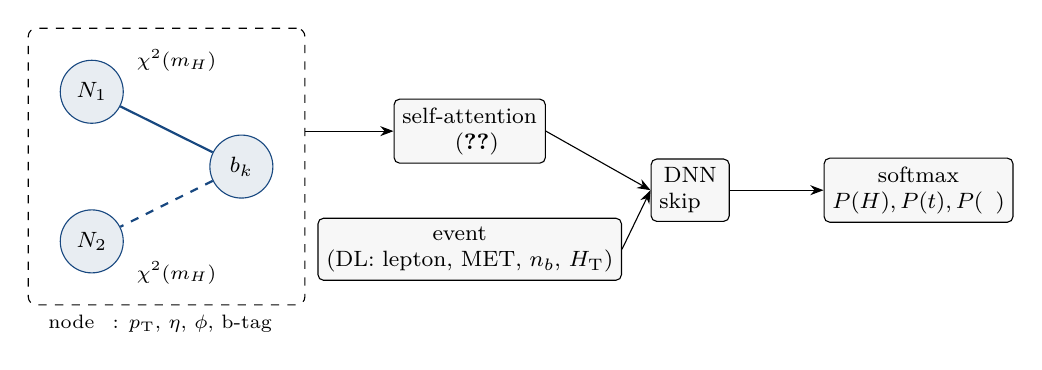
\begin{tikzpicture}[font=\footnotesize, >=Stealth,
  jet/.style={circle, draw=accent, fill=accent!10, minimum size=8mm, inner sep=0pt},
  box/.style={draw, rounded corners=2pt, align=center, inner sep=3pt, fill=black!3}]
\node[jet] (b)  at (0,0)       {$b_k$};
\node[jet] (n1) at (-1.9,0.95) {$N_1$};
\node[jet] (n2) at (-1.9,-0.95){$N_2$};
\draw[accent, thick] (b) -- (n1);
\draw[accent, thick, dashed] (b) -- (n2);
\node[font=\scriptsize, anchor=west] at (-1.45,1.35) {$\chi^2(m_H)$ 최소};
\node[font=\scriptsize, anchor=west] at (-1.45,-1.35) {$\chi^2(m_H)$ 둘째};
\node[draw, dashed, rounded corners=3pt, fit=(b)(n1)(n2), inner sep=4mm] (g) {};
\node[font=\scriptsize, anchor=north] at (g.south) {node 입력: \pt, $\eta$, $\phi$, b-tag 값};
\node[box] (att) at (2.9,0.45)  {self-attention\\ 식~\eqref{eq:mva-gat}};
\node[box] (ev)  at (2.9,-1.05) {event 변수\\ (DL: lepton, MET, $n_b$, \HT)};
\node[box] (dnn) at (5.7,-0.3)  {DNN\\ skip 연결};
\node[box] (out) at (8.6,-0.3)  {softmax\\ $P(H), P(t), P(\text{기타})$};
\draw[->] (g.east |- att) -- (att);
\draw[->] (att.east) -- (dnn.west);
\draw[->] (ev.east) -- (dnn.west);
\draw[->] (dnn) -- (out);
\end{tikzpicture}
\caption{GATJA 의 한 b jet 판정(AN-2022/122 Fig.~36--37, GATJA 발표 p.8--9 를 단순화). b jet 마다 반복해 최대 8 개 b jet 의 24 개 출력을 만든다.}
\label{fig:mva-gatja}
\end{figure}

\subsection{입력 변수 묶음과 우리 Tree}\label{sec:mva-an-inputs}

DL 의 Table 43 은 baseline 을 통과한 모든 event 에서 계산한 변수 목록이다\src{AN-22-122 v26, PDF p.50, Table 43}. SL 의 333 개는 부록 B 에 있다
(125 개만 나열됨). 표~\ref{tab:mva-inputs} 는 Table 43 의 묶음이 FH 에 쓰이는지와 우리 Tree v1 의 이름이다(정의는 \ref{ch:reco}장,
branch 목록은 부록~\ref{ch:treev1}).

\begin{table}[htbp]
\centering
\caption{AN Table 43 의 묶음과 우리 Tree v1(STEP 27). FH 에서 lepton·MET 관련 양은 뺀다.}
\label{tab:mva-inputs}
\footnotesize
\begin{tabularx}{\linewidth}{@{}p{24mm} L L@{}}
\toprule
묶음 & AN 변수 & Tree v1 / 기존 branch \\
\midrule
다중도 & $N_{\mathrm{jets}}, N_{\mathrm{bjets}}, N_{\mathrm{light}}$ & \code{nJets}, \code{nbJets}, \code{lightjetNumber}, (\code{nLooseJets}) \\
4-운동량 & jet 1--6, b jet 1--6 의 \pt, $|\eta|$; lepton 1, 2 & \code{jetPt}, \code{jetEta}, \code{jetPhi}, \code{jetMass}, \code{bTagScore} 벡터 → 내보내기 도구가 열로(lepton 은 FH 에 없음) \\
\HT & $H_T, H_T^b, H_T^{\mathrm{light}}$; $H_T^{\mathrm{lep}}, S_T$ & \code{HT}, \code{bjetHT}, \code{lightjetHT}(lepton 쪽은 제외) \\
질량 & $m^{\mathrm{avg}}_{j,b,\mathrm{light}}$, $(m^2)^{\mathrm{avg}}_b$, $m^{\max p_T}_{jjj,jbb}$; $m_{\mu\mu}, m_{ee}$ & \code{jetAverageMass}, \code{bjetAverageMass}, \code{lightjetAverageMass}, \code{bjetAverageMassSqr}, \code{maxPTmassjjj}, \code{maxPTmassjbb} \\
각도 & $\Delta\eta^{\mathrm{avg}}_{jj,bb}$, $\Delta\eta^{\max}_{bb}$, $\dR^{\mathrm{avg,min}}_{jj,bb}$, 최소 $\dR$ 쌍의 질량·\pt & \{\code{average},\code{min},\code{max}\}\code{DeltaR}, \{\code{average},\code{max}\}\code{DeltaEta}, \code{minDeltaRMass}, \code{minDeltaRpT} × \{jj, bb, bj\} = 21 개 \\
$\chi^2$ 쌍 & $\chi^2_{HH,ZZ,ZH}$, $m_{H1,H2}$, $m_{Z1,Z2}$, $m_{ZH}$, $p_T(H_{1,2})$ & \code{chi2Higgs}, \code{chi2Z}, \code{chi2HiggsZ}, \code{invMassH1/H2}, \code{invMassZ1/Z2}, \code{invMassHiggsZ1/Z2}, \code{PTH1/PTH2}(AN 의 jet 선택, $n_M\ge2$ 로 넓힘) \\
event shape & aplanarity, centrality, sphericity, $S_\perp$, C, D(jet, b jet) & \code{aplanarity} … \code{eventD}, \code{centrality} 와 \code{bjet} 판 \\
Table 43 밖 & Fox–Wolfram $H_0$--$H_4$, $R_i$; jet b-tag 값; GATJA 24 & \code{H0}--\code{H4}, \code{R1}--\code{R4}, \code{bjetH0}… ; \code{bTagScore}, \code{jetBTagWP}; GATJA 는 계획 \\
FH 추가 & — & \code{invMassHadW}($m_{qq}$, QCD 영역의 축), \code{metPhi} \\
\bottomrule
\end{tabularx}
\end{table}

\begin{note}[AN 안의 엇갈림 — 우리 정의를 고정할 때 주의]
(1) 본문은 event shape 변수를 "DL 에서만" 쓴다지만 SL 상위 50 에 jet aplanarity(4 위)와 $H_1$(8 위)이 있다\src{AN-22-122 v26, PDF p.52, 108}.
(2) SL Table 50 의 머리말은 "($\ge4$ jets, $\ge3$ b-tags)" 다\src{AN-22-122 v26, PDF p.109}. (3) DL node 는 Fig.~87 이 7 개, 본문·혼동 행렬은 6 개다
\src{AN-22-122 v26, PDF p.115--117}. (4) $\chi^2$ 의 $\sigma$ 는 "JER 의 함수" 라고만 한다\src{AN-22-122 v26, PDF p.49} — 우리는 옛 식을 두고 미결로 남겼다\src{STEP 27}.
\end{note}

% -----------------------------------------------------------------------------
\section{참고: ttH(bb) FH 의 판별 변수}\label{sec:mva-tth}

ttH(bb) FH 는 범주(7 jet, 8 jet, $\ge9$ jet; 모두 $\ge4$ b)마다 \textbf{이진} ANN 을 쓴다: 목표는 ttH(\Hbb) 대 QCD multijet 이다. tt+jets 를 더한
다중 분류로도 큰 개선이 없었다\src{AN-19-094 v20, PDF p.113}. QCD MC 는 SR 에서 모델링이 나쁘고 통계가 적어 학습에 쓰지 않고, 대신
\textbf{TR(2 M + $\ge2$ 추가 L) 의 data} 에 TF\textsubscript{loose} 보정을 곱해 배경 class 로 쓴다(TR 은 QCD 가 80 \% 이상, 다음이 tt+LF)
\src{AN-19-094 v20, PDF p.113}. 신호는 SR 의 ttH MC 중 event number 홀짝의 절반만 학습·검증에 쓰고 나머지 절반을 fit 에 쓴다. 통계를 늘리려고 세 해를
합쳐 학습하고 신호는 lumi 비로 가중했으며, 해마다 입력 모양이 같음을 확인했다\src{AN-19-094 v20, PDF p.113}. 설정은 표~\ref{tab:mva-tth}.

\begin{table}[htbp]
\centering
\caption{ttH(bb) FH ANN(AN-19-094 v20 Table 66, PDF p.114; 성능 Fig.~61, PDF p.115).}
\label{tab:mva-tth}
\small
\begin{tabularx}{\linewidth}{@{}l C C C@{}}
\toprule
 & 7 jet, $\ge4$ b & 8 jet, $\ge4$ b & $\ge9$ jet, $\ge4$ b \\
\midrule
입력 수 & 19 & 21 & 21 \\
구조 & \multicolumn{3}{c}{3 층 × 100 node, ReLU, 출력 sigmoid, binary CE, Adam($10^{-4}$)} \\
L2 / dropout & $10^{-4}$ / 0.5 & $5\cdot10^{-4}$ / 0.6 & $10^{-4}$ / 0.5 \\
batch & 5000 & 20000 & 5000 \\
AUC(검증 표본, ANN / MEM 단독) & 0.81 / 0.77 & 0.80 / 0.76 & 0.78 / 0.70 \\
AUC(VR, ttH 대 추정 QCD) & 0.75 & 0.74 & 0.73 \\
AUC(VR, ttH 대 tt+jets) & 0.62 & 0.62 & 0.63 \\
\bottomrule
\end{tabularx}
\end{table}

\textbf{b-tag 값을 입력에서 뺀 이유}. 입력은 "b-tagging 값과의 직접 상관을 피해" 배경 추정 방법과 맞도록 골랐다\src{AN-19-094 v20, PDF p.114}.
입력 검증의 첫 단계는 TR, CR, SR 에서 변수의 모양이 같은지다: QCD 학습 표본은 TR 에서, 신호와 평가는 SR 에서 오기 때문에, 영역을 가르는 양과
상관된 변수는 쓸 수 없다\src{AN-19-094 v20, PDF p.156}. 예로, "b jet 의 평균 b-tag 값" 은 7 jet 의 m\textsubscript{qq} 중앙창에서 평균이 TR 0.438,
CR 0.574 로 다르다(그림 범례)\src{AN-19-094 v20, PDF p.157, Fig.~89}. BLR 도 FH 에서는 쓰지 않았다\src{AN-19-094 v20, PDF p.379, Table 154}. 남은 입력은 MEM, Fox–Wolfram 모멘트,
aplanarity·sphericity, jet 쌍의 $\Delta\eta$·$\dR$ 통계, b-tag 순위 1·2 jet 의 $\eta$ 같은 운동학이다(범주마다 19/21/21 개)\src{AN-19-094 v20, PDF p.114, 386--398}.
"b-tag 순위로 고른 jet 의 운동학" 은 b-tag 값은 아니지만 b-tag 와 상관될 수 있어 이것도 모양 검사를 통과해야만 남았다.

\textbf{MEM}. 행렬 원소 방법의 판별 값은 $P_{S/B}=w_S/(w_S+\kappa\,w_B)$ 이고, $w$ 는 jet 과 parton 의 모든 순열에 대해 위상 공간·행렬 원소·전달 함수로
적분한 무게의 합이다($S$ = ttH, $B$ = tt+bb; 기본 $\kappa=0.1$)\src{AN-19-094 v20, PDF p.65}. FH 는 7·8 jet 에서 W 의 quark 하나를 잃은 가설
3W2H2T, $\ge9$ jet 에서 완전 재구성 4W2H2T 를 쓰고 $\kappa=0.065$ 다. 모든 영역에서 b-tag 값 상위 4 jet 을 b 로 둔다(영역 사이 정의를 같게)
\src{AN-19-094 v20, PDF p.66, Table 54}. 이전 FH 분석은 MEM 을 최종 판별 변수로 썼고 이번에는 ANN 의 입력이다\src{AN-19-094 v20, PDF p.114}.

\begin{note}[ttH FH 에서 배울 점]
FH 의 QCD 는 MC 가 아니라 data(TR)로 학습하고, 그 대가로 입력은 b-tag 와 무관해야 한다 — 아니면 TR(낮은 b-tag)에서 배운 QCD 모양이 SR 에서 성립하지
않고 CR 의 QCD template(\ref{ch:qcd}장)의 출력도 SR 과 달라진다. ANN 은 tt+jets 를 거의 가르지 못했다(VR AUC 0.62--0.63). ttHH 는 tt+bb·ttZH·ttZZ
를 가르는 것이 핵심이라 AN-2022/122 의 다중 분류를 따라야 한다(우리 판단).
\end{note}

% -----------------------------------------------------------------------------
\section{우리 FH 분석의 설계}\label{sec:mva-ours}

\subsection{원칙}\label{sec:mva-ours-principle}

사용자 방향(2026-10-10): "SWAN project의 전체적인 구조를 참조하되 머신러닝 학습 방향은 ttHH AN을 기반으로 FH에 맞게 적용해야 한다. … 억지로 변형할
바엔 Run2 기준에 맞추는게 적절함."\src{D-2026-10-10-B}. 그래서 방법(class, 구조, 학습 절차, 전처리, 홀짝 분할, epoch 선택)은 AN SL DNN 에서 가져오고 \tagan, FH 가 요구하는 것(QCD class,
lepton·MET 변수 제거, b-tag 입력의 제약)과 Run 3 가 요구하는 것(2024 의 b-tag 입력 형식)만 바꾼다 \tagrunthree. SWAN 의 옛 FH 노트북은 코드
구조만 참고한다(\S\ref{sec:mva-ours-swan}). 학습은 Run 2 전체와 2024 가 기본이고, GPU 는 SWAN 이 기본, 필요하면 KNU GPU 다\src{D-2026-10-10-B}.

\subsection{class 와 fit node}\label{sec:mva-ours-classes}

표~\ref{tab:mva-classes} 는 제안이다\src{PLAN\_ML\_SYST §9.2}. 학습 class 는 SL 의 9 node 에 QCD 를 더한 10 개이고, fit 에서 node 를 묶는 방식은 AN 과
승인 발표의 최종 모델을 따른다 \tagplan.

\begin{table}[htbp]
\centering
\caption{FH DNN 의 학습 class 와 fit node(제안). 2024 의 tt+mb/tt+nb 는 tt+nb lookup 이 생길 때까지 나눌 수 없다.}
\label{tab:mva-classes}
\footnotesize
\begin{tabularx}{\linewidth}{@{}l L L l@{}}
\toprule
학습 class & 표본(Run 2 / 2024) & 비고 & fit node \\
\midrule
ttHH & \code{TTHHTo4b}(v15 없음) / \code{TTHH-HHto4B} & 신호 & ttHH \\
ttH & ttH(bb) & & ttH \\
ttZH, ttZZ, ttZ & \code{TTZHTo4b}, \code{TTZZTo4b}(v15 없음), ttZ(Z→qq) / 2024 중앙 & Run 2 v15 의 ttZ 는 \code{TTZToBB} 대신 \code{TTZToQQ} & ttZ(1 bin 가능) \\
tt+lf, tt+cc & tt 5FS(FH, SL, DL 모두) & lepton 을 놓친 SL·DL 도 FH 선택에 들어온다 & tt \\
tt+mb, tt+nb & 4FS tt+bb, LO tt4b(stitching) & 2024: tt+$\ge$3b 는 tt+B 안(lookup 없음) & ttb(또는 tt) \\
QCD & TR data $\times$ TF\textsubscript{loose} & ttH FH 방식, \ref{ch:qcd}장 & QCD \\
\bottomrule
\end{tabularx}
\end{table}

근거: 표본 이름과 부재\src{NtupleForge 04\_mc\_request §1, §3}, tt 의 세 붕괴 채널을 모두 배경으로 쓰는 이유\src{NtupleForge 04\_mc\_request §2},
2024 의 tt+nb\src{D-2026-10-05-C}. QCD node 로 간 event 는 QCD 가 많은 범주가 되어 fit 에서 QCD 정규화를 잡는 데 쓰인다\src{PLAN\_ML\_SYST §9.2}.
TR 의 data 는 학습에만 쓰고 QCD template 은 CR(3 M + $\ge1$ L)에서 만들므로(ttH FH 방식), 같은 data event 가 학습과 template 에 동시에 들어가지 않는다.

\subsection{입력 변수와 b-tag 정보 — 가장 큰 미결}\label{sec:mva-ours-btag}

후보는 Table 43 과 부록 B 중 FH 에 있는 것(표~\ref{tab:mva-inputs})이다. 문제는 b-tag 정보다. AN SL 은 b-tag 값($d_3$…$d_6$)과 BLR 을 상위에 쓰고,
DL 은 jet b-tag 값과 (b-tag 값을 node 입력으로 받는) GATJA 출력을 쓴다\src{AN-22-122 v26, PDF p.108, 116}. 반면 FH 의 QCD 는 TR→CR→SR 의
b-tag 외삽으로 추정하므로(\ref{ch:qcd}장), 입력이 b-tag 와 직접 상관되면 그 외삽이 깨진다(\S\ref{sec:mva-tth}). 선택지는 셋이다.
\begin{enumerate}
\item AN 그대로 b-tag 값을 쓴다 — QCD 의 TR/CR 모양이 SR 과 달라질 위험이 크다.
\item ttH FH 처럼 b-tag 값을 모두 뺀다 — QCD 추정은 안전하지만 tt+bb, ttZH/ttZZ 분리력을 잃는다(AN 상위 변수의 다수가 빠짐).
\item \textbf{TR·CR·SR 모양 동등성 검사(중앙창과 사이드밴드)를 통과한 변수만} 쓴다(권고)\src{PLAN\_ML\_SYST §8 8, §9.2}\src{ROADMAP\_FH §6 2}.
\end{enumerate}
$\chi^2$ 쌍짓기도 검사 대상이다: AN 규칙에서 $n_M=3$ 이면 넷째 jet 이 L--M jet 이고, 우리가 넓힌 $n_M=2$(TR) 에서는 셋째·넷째가 L--M jet 이다
\src{STEP 27}. 결정은 사용자 몫이다 \tagopen.

\textbf{2024 의 b-tag 입력} \tagrunthree. 2024 에는 fixed-WP SF 만 있어(b jet 만, \ref{ch:btag}장) WP 칸 안의 점수 모양은 보정되지 않는다. 그래서 연속 점수
대신 WP 칸을 입력으로 쓰는 것이 SF 와 맞는다 — BTV 문서도 "WP-binned information may be a BDT/DNN input" 이라고 한다\src{D-2026-10-10-A}.
Tree v1 의 \code{jetBTagWP} 는 네 칸(\textless L, [L, M), [M, T), $\ge$T)이다\src{ttHHanalyzer\_unified.cc, fillTreeV1\_}. PLAN 은 XT, XXT 까지 여섯 칸을
제안했으므로\src{PLAN\_ML\_SYST §5.3}, 더 잘게 필요하면 내보내기 도구가 \code{bTagScore} 에서 다시 만든다. Run 2(DeepJet)와 2024(UParTAK4)는 점수의
정의가 달라 연도를 묶어 학습할 때 같은 열에 넣을 수 없다.

\subsection{연도 처리}\label{sec:mva-ours-years}

AN 은 연도별로 학습했고\src{AN-22-122 v26, PDF p.106}, ttH FH 는 세 해를 합쳤다\src{AN-19-094 v20, PDF p.113}. 권고는 AN 대로 연도(era)별 학습으로 시작하고
통계가 모자라면 Run 2 를 묶는 것이다\src{PLAN\_ML\_SYST §8 9}. 2024 는 13.6\TeV, 다른 tagger, PUPPI jet 이라 Run 2 와 따로 학습하는 것이 자연스럽다(우리 판단).
연도를 묶을 때는 연도 표지를 입력에 넣거나 lumi 비로 가중하고, ttH FH 처럼 연도별 입력 모양을 먼저 비교한다 \tagopen.

\subsection{학습 데이터}\label{sec:mva-ours-data}

\begin{table}[htbp]
\centering
\caption{학습 표본의 현황(2026-10-10). 출처: PLAN\_ML\_SYST §10, NtupleForge 04\_mc\_request §1, D-2026-10-02-A.}
\label{tab:mva-data}
\footnotesize
\begin{tabularx}{\linewidth}{@{}l l l l L@{}}
\toprule
연도 & 신호 TTHH & TT4b & TTZH·TTZZ & 상태 \\
\midrule
2024(Summer24 v15) & 중앙 \code{TTHH-HHto4B} & \code{TT4B} & 중앙 & 생산 끝 — 첫 학습 표본 \\
2018(UL v15) & 없음 & 없음 & 없음 & MC·Data 생산 끝; 다섯 표본(표의 넷과 \code{THW})은 중앙 요청(2026-09-14, 답장 기록 없음)과 enriched 사설 생산 병행 \\
2016·2017(UL v15) & 없음 & 없음 & 없음 & hadronic 생산 전 \\
\bottomrule
\end{tabularx}
\end{table}

Run 2 의 다섯 표본은 v9 에는 있고 v15 에는 없으며 MiniAODv2 부모(신호 2016pre/2016post/2017/2018 = 5.0M/4.8M/9.9M/9.6M event)에서 NANO 단계만
남았다\src{NtupleForge 04\_mc\_request §1}. 2017 v9 ntuple 은 KNU 에서 지워졌다\src{D-2026-10-05-D}. 그래서 첫 기준선은 2024 로 만든다(권고)
\src{ROADMAP\_FH §6 3}: trigger·b-tag SF 를 켠 2024 SF main 셋을 STEP 27 실행 파일로 돌린 출력이 control plot 과 첫 학습 표본을 겸한다\src{ROADMAP\_FH §2}.

\subsection{Tree v1 이 이미 주는 것}\label{sec:mva-ours-tree}

Tree 에는 baseline 선택(\code{selectObjects})을 통과한 모든 event 가 들어간다 — TR(2 M)도 baseline($n_b\ge2$) 안이고, $n_b\ge3,4$ 와
Higgs 질량창 단계는 지금 관찰 전용이다\src{ttHHanalyzer\_unified.cc, process, kCutSequence}.
\begin{itemize}
\item \textbf{DNN 입력} \tagimpl\tagtest: jet 벡터(\code{jetPt}, \code{jetEta}, \code{jetPhi}, \code{jetMass}, \code{bTagScore}, \code{jetBTagWP}, \code{hadFlavs})와
  event 변수 약 75 개(표~\ref{tab:mva-inputs})\src{STEP 27}.
\item \textbf{GATJA 표지}(MC): \code{jetGenMatch}(0 없음, 1 H→b, 2 t→b, 3 W→q, 4 Z→q)와 \code{jetGenMotherIdx}(어미의 첫 사본 번호 — 같은 Higgs 의 두 b 가 같은 값).
  hard-process 의 마지막 사본 quark 와 $\dR<0.4$ 로, 가까운 순서로 한 번씩 짝짓는다\src{GenMatch.h}. \code{bjetHiggsMatched} = (값 1),
  \code{bjetTopMatched} = (값 2). 규칙은 PROPOSED\src{PLAN\_ML\_SYST §8 4}.
\item \textbf{weight 와 분할}: \code{evtWeight}(production: 토글로 켠 SF 만 곱함 — 기본은 trigger SF 만), \code{evtWeight_btagSF}(trigger SF 와 b-tag SF 를 언제나),
  \code{evtWeight_full}(+norm reweight)\src{ttHHanalyzer\_unified.cc, selectObjects}, 계통 weight(\ref{ch:syst}장), \code{genTtbarId}·\code{expandedTtbarId}(tt class),
  \code{eventNumber}(홀짝).
\item \textbf{없는 것}: 내보내기 도구(\file{tools/ml/}: \code{export_tree.py}, \code{gatja_inputs.py}), GATJA 의 $\chi^2(m_H)$ 이웃 번호, BLR(flavour 별 b-tag pdf
  필요)\src{PLAN\_ML\_SYST §5.1, §9.4}. 표지와 weight 는 입력 열과 따로 둔다 — SWAN DL 판은 \code{weight} 와 gen 매칭 표지가 입력에 섞여 쓸 수 없었다
  \src{PLAN\_ML\_SYST §2.5}.
\end{itemize}

\subsection{GATJA 의 FH 판}\label{sec:mva-ours-gatja}

node·이웃·표지의 정의는 채널과 무관하다. 바꿀 것은 event 변수다: lepton·MET 대신 \code{HT}, \code{bjetHT}, \code{lightjetHT}, \code{nJets}, \code{nbJets}, 평균 질량들
(필요하면 \code{invMassHadW})을 넣고, stage 1 을 FH 표본으로 다시 학습한다(GPU)\src{PLAN\_ML\_SYST §2.2, §9.3} \tagplan. FH 의 final state 는 b 6 개와 W 의 light
quark 4 개, 즉 parton 10 개다. 그래프는 b-tag 된 jet(최대 8 개)만 node 로 쓰므로 W jet 은 mistag 될 때만 들어와 "기타" 가 된다. 우리 표지에는
W→q(값 3)와 Z→q(값 4)가 따로 있어 class 를 넓힐 수 있지만 AN 의 3 class 로 시작한다\src{PLAN\_ML\_SYST §9.3}. stage 2(GATJA 출력만으로 ttHH 대
ttZH+ttZZ)는 확인용으로 그대로 둔다. GATJA 의 node 입력에도 b-tag 값이 있으므로 \S\ref{sec:mva-ours-btag} 의 검사가 똑같이 걸린다. 공개 코드는
저장소 밖의 \file{snowttHHtools.py} 를 import 하고 DL allSys ntuple 경로를 가정하며, 학습된 weight 파일은 없다\src{PLAN\_ML\_SYST §2.2}.

\subsection{학습 환경: SWAN 과 KNU GPU}\label{sec:mva-ours-env}

표본은 KNU \file{/pnfs} 의 merge 출력 → 내보내기 도구 → EOS(CERNBox)로 xrdcp → SWAN 에서 학습한다\src{PLAN\_ML\_SYST §10}. GATJA 는
Python ≥ 3.10, TensorFlow, tensorflow-addons(LAMB), tf-models-official 이 필요하고, tensorflow-addons 는 개발이 끝난 패키지라 SWAN 의 TF 판과의 호환을
먼저 확인한다\src{PLAN\_ML\_SYST §2.2, §10}. AN SL DNN 은 Adam 이므로 FH DNN 기준선에는 이 의존이 없다(우리 판단).

\subsection{SWAN 의 옛 FH 시험 판에서 가져오는 것}\label{sec:mva-ours-swan}

SWAN 의 FH 노트북 마지막 판 V3(2024-09)은 13 class(QCD MC, tttt, tttW, ttWH, ttWW, ttWZ 포함), 입력 112 개(옛 FH 이름, b-tag 값 없음),
Robust → Standard → MinMax 변환, Dense 523(LeakyReLU, dropout 0.1) → 523 → 261 → 130 → softmax, Adam $3\times10^{-6}$, batch 512, 150 epoch,
event weight 없이 표본별로 덜어낸 뒤 균형 class weight 였다\src{PLAN\_ML\_SYST §2.4}. 여기서 \textbf{가져오는 것}은 노트북의 흐름(읽기 → 전처리 → 모델 →
학습 → 혼동 행렬·손실 곡선), \code{Channel} 스위치, 출력 히스토그램 저장 같은 구조뿐이고, class·입력·구조·학습 절차·분할은 표~\ref{tab:mva-an-dnn} 의
AN SL 판을 따른다 \tagan.

\begin{andiff}[이름 함정 — 옛 FH ntuple 과 DL 새 이름]
옛 FH ntuple 과 옛 DL template 은 모든 branch 앞에 \code{b} 를 붙였다: \code{bjetPT1} 은 \textbf{첫 jet}, \code{bbjetPT1} 이 첫 b jet, \code{baplanarity}·\code{bH0} 는
jet 전체의 양이다. DL 새 이름에서는 \code{bjetPT1} 이 첫 b jet, \code{baplanarity}·\code{bH0} 가 b jet 의 양이다. 우리 Tree v1 은 DL 새 이름을 따르되 b jet 양에
\code{bjet} 접두를 쓴다(\code{bjetH0})\src{PLAN\_ML\_SYST §3}. V3 노트북을 새 표본에 쓸 때는 대응표(PLAN 부록 A)로 바꿔야 하고, 섞으면 조용히 틀린 입력이 된다.
\end{andiff}

% -----------------------------------------------------------------------------
\section{검증 계획}\label{sec:mva-validation}

뼈대는 AN 이 보인 셋이다: DL CR($n_{\mathrm{jet}}\ge4$, $n_b=2$, 2 lepton)과 SR 의 DNN 입력 Data/MC\src{AN-22-122 v26, PDF p.73--81},
Hbb convener 의 제안으로 본 SL SR 의 DNN 입력 Data/MC\src{AN-22-122 v26, PDF p.82--105}, node 별 학습/test 비교(부록 E). 입력 하나하나에는 신호가
보이지 않으므로 SR 의 입력은 data 로 본다. 아래는 모두 \tagplan 이다.
\begin{enumerate}
\item \textbf{입력의 Data/MC}: lepton CR(μCR, eCR; QCD 가 억제된 영역)과 FH baseline 에서 모든 입력의 Data/MC. \file{plotter/make_plots.py} 의
  \code{--tree-v1} 이 Tree v1 의 ML 입력 30 개와 $m_{qq}$, 모두 31 개를 그린다 \tagimpl\src{plotter/make\_plots.py, TREE\_HISTS\_V1}\src{STATUS 10-10 (3)}.
\item \textbf{영역 사이 모양 동등성}: QCD 가 지배하는 data 에서 TR, CR, SR 의 정규화된 모양(m\textsubscript{qq} 중앙창과 사이드밴드) — ttH FH §10.1 의
  방법(\S\ref{sec:mva-ours-btag}; \src{AN-19-094 v20, PDF p.157, Fig.~89}).
\item \textbf{과적합과 closure}: class 별 학습/test 출력의 KS 검정(AN 부록 E 에 해당); 홀짝을 바꾼 모델·연도별 모델의 출력이 통계 안에서 같은지.
\item \textbf{b-tag SF 변형에 대한 강건성}: Run 2 는 \code{bTagWeight_<src>_up/down} 16 개, 2024 는 \code{bTagWeight_up/down} 과 비교 weight
  (\code{bTagWeight_oldRule}, \code{bTagWeight_cAsB})로 node 별 template 이 얼마나 움직이는지. b-tag 와 상관된 입력이 많을수록 크게 움직인다.
\item \textbf{GATJA}: 표지 검증(ttHH MC 에서 H 에 매칭된 b jet 쌍의 질량이 125\GeV 근처, \src{PLAN\_ML\_SYST §5.2}), jet 단위 혼동 행렬, stage 2.
\item \textbf{출력의 Data/MC}: 신호가 적은 bin(과 QCD node)에서만 data 를 본다 — 신호에 민감한 bin 은 가린다(D-2026-10-02-E, \ref{ch:stats}장).
\end{enumerate}

% -----------------------------------------------------------------------------
\section{변경 이력}\label{sec:mva-history}

2024-06--09: SWAN 의 FH·DL 겸용 DNN 노트북 다섯 판(입력 202 → 112 개)\src{PLAN\_ML\_SYST §2.4}. 옛 analyzer 의 DNN branch 는 2026-06-11 백업에서
이미 239 줄 중 203 줄이 주석, 지금은 지워짐\src{PLAN\_ML\_SYST Bottom line 1}. 2026-10-10: D-2026-10-10-B 와 STEP 27 의 Tree v1(옛 helper 의 결함을 새 함수로 고침).

% -----------------------------------------------------------------------------
\section{미결 사항}\label{sec:mva-open}

\begin{openq}
\begin{enumerate}
\item \textbf{DNN·GATJA 입력의 b-tag 정보}: 쓸지, 모양 검사를 통과한 것만 쓸지(권고), 모두 뺄지 — QCD 방법(\ref{ch:qcd}장)과 함께. 2024 의 WP 칸 수(L, M, T 대 XT, XXT 까지).
\item \textbf{QCD class}: TR data 의 정의(SR 이 $n_M\ge5$ 면 TR 도 옮기는가), TF\textsubscript{loose} 적용, tt 기여를 빼는가.
\item \textbf{Run 2 학습 데이터}: v15 의 신호·TT4b·TTZH·TTZZ·THW 부재(중앙 요청 답장 또는 enriched 생산 대기) — 그 전에는 2024 로만.
\item \textbf{연도와 tt class}: 연도별 모델(AN) 대 묶음; 2024 는 tt+nb lookup 이 없어 tt+mb/tt+nb 를 나눌 수 없다(D-2026-10-05-C).
\item \textbf{GATJA 의 FH 판}: parton 10 개(b 6, light 4)에서의 이웃 정의, W class, event 변수, GPU 시간, tensorflow-addons 호환.
\item \textbf{학습 weight·분할·정의}: event·class weight 와 음의 weight; 홀짝 한 방향(AN) 대 2-fold; $Z_A$ 의 $\sigma_b=0.1$ 이 절대값인지(확인 못 함);
  $\chi^2$ 의 $\sigma$; jet 7, 8 의 운동학을 더할지.
\end{enumerate}
\end{openq}

% =============================================================================
% 10 장 — 계통 불확도
% 작성 2026-10-10 (AN_KR v0.1). 근거: AN-2022/122 v26 §8.2(Table 52–53, Table 9, App. C);
% AN-19-094 v20 §3.1, §9(Table 79), §11; docs/PLAN_ML_SYST.md §5–§6; docs/reference/LUMI_SOURCES.md;
% DECISIONS D-2026-10-05-A, D-2026-10-08-A, D-2026-10-10-A/B; STEP 26, STEP 27; 코드(ttHHanalyzer_unified.{h,cc},
% src/CorrectionsManager.cc, plotter/stack_plotter.C, TriggerStudy/docs/ARCHITECTURE.md).
% =============================================================================
\chapter{계통 불확도}\label{ch:syst}

계통 불확도(systematic uncertainty)는 측정값을 예측과 비교할 때 "예측 자체가 얼마나 틀릴 수 있는가" 를 fit 에 넣는 장치다. 이 장은 먼저 개념 —
정규화(lnN)와 모양(template morphing) 불확도, 연도·과정 사이 상관, weight 로 만드는 변형과 다시 돌려야 하는 변형(JES·JER), data 와 MC 의 통계
불확도 — 을 정리한다. 이어서 Run 2 ttHH AN 의 전체 목록(Table 53)과 지배적인 항목, ttH(bb) FH 가 더한 FH 고유 항목(QCD 추정, hadronic trigger SF,
tt+B 정규화)을 옮긴다. 그다음 출처마다 우리 코드의 지금 상태(STEP 27 의 Tree weight)와 계획을 표로 보이고, 지금 control plot 의 통계 오차가
어떻게 그려지는지와 미결 사항을 적는다. 요약하면 weight 로 만드는 변형은 Tree 에 기록되기 시작했고(\tagimpl\tagtest, 실제 표본 실행 전),
JES·JER 변형, datacard, QCD 추정의 불확도는 \tagplan 이다.

% -----------------------------------------------------------------------------
\section{개념}\label{sec:syst-concepts}

\subsection{nuisance parameter: 정규화와 모양}\label{sec:syst-np}

\ref{ch:stats}장의 binned likelihood 에서 계통 불확도의 원천 $k$ 마다 nuisance parameter $\theta_k$ 를 두고, 보조 측정(calibration)의 결과를
제약항 $p(\tilde\theta_k|\theta_k)$ 로 곱한다. 관례상 $\theta_k$ 는 단위 Gaussian 으로 정규화해 $\theta_k=\pm1$ 이 원천의 $\pm1\sigma$ 변형이 되게 한다.
예측 수율 $\nu_i$(bin $i$)가 $\theta_k$ 에 어떻게 의존하는지가 두 종류를 가른다.

\textbf{정규화(rate) 불확도}는 과정의 총 수율만 바꾼다. combine 의 \code{lnN} 은
\begin{equation}
  \nu(\theta)=\nu_0\,\kappa^{\theta},\qquad \theta\sim\mathcal{N}(0,1)
  \quad\Longrightarrow\quad \ln\nu\ \text{가 Gaussian(log-normal)},
  \label{eq:syst-lnN}
\end{equation}
이고, 비대칭(datacard 의 \code{0.95/1.05} 꼴)이면 $\theta>0$ 에서 $\kappa_{\mathrm{up}}^{\theta}$, $\theta<0$ 에서 $\kappa_{\mathrm{down}}^{-\theta}$ 를 쓴다
($\theta=-1$ 이면 $\nu_0\kappa_{\mathrm{down}}$). 곱셈 꼴이라 수율이 음이 되지 않고, $\kappa-1$ 이
작으면 상대 불확도 $\kappa-1$ 의 Gaussian 과 같다. 예: 2017 lumi 0.82 \% 는 두 성분 \code{lumi_13TeV_151617_l} = 1.0055,
\code{lumi_13TeV_15161718_l} = 1.0061 로 들어간다(제곱합 0.82 \%)\src{LUMI\_SOURCES §2}.

\textbf{모양(shape) 불확도}는 bin 마다 다르게 움직인다. 원천을 $\pm1\sigma$ 바꾼 template $\nu_i^{\pm}$ 를 만들고, 그 사이를 bin 마다 보간한다
(vertical template morphing). 가장 단순한 꼴은
\begin{equation}
  \nu_i(\theta)=
  \begin{cases}
    \nu_i^0+\theta\,(\nu_i^{+}-\nu_i^{0}), & \theta\ge0,\\
    \nu_i^0+\theta\,(\nu_i^{0}-\nu_i^{-}), & \theta<0,
  \end{cases}
  \label{eq:syst-morph}
\end{equation}
이다(그림~\ref{fig:syst-morph}). combine 은 $|\theta|<1$ 에서 미분이 이어지도록 다항식으로 매끄럽게 잇고 바깥은 선형으로 외삽한다. template 의
총 수율이 변하면 정규화 효과도 함께 들어간다. 한쪽 template 만 있으면(예: ttH FH 의 TF\textsubscript{loose}, 아래) "단측" 불확도가 된다.
AN 의 SL 은 rate 계통을 datacard 에 직접, shape 계통은 up/down template 으로 넣었다\src{AN-22-122 v26, PDF p.119}.

\begin{figure}[htbp]
\centering
\begin{tikzpicture}[font=\footnotesize, >=Stealth, x=1.35cm, y=1.25cm]
\draw[->] (-2.4,0) -- (2.5,0) node[right]{$\theta$};
\draw[->] (0,-0.1) -- (0,3.1) node[above]{$\nu_i(\theta)$};
\foreach \x in {-2,-1,1,2} \draw (\x,0.05) -- (\x,-0.05) node[below]{$\x$};
\draw[accent, thick] (-2,0.8) -- (0,1.6) -- (2,2.8);
\draw[gray, dashed, domain=-1:1, samples=40] plot (\x, {1.6+0.5*\x+0.1*\x*\x});
\fill (-1,1.2) circle (1.6pt) node[below right]{$\nu_i^-$};
\fill (0,1.6) circle (1.6pt) node[above left]{$\nu_i^0$};
\fill (1,2.2) circle (1.6pt) node[below right]{$\nu_i^+$};
\node[accent, anchor=west, font=\scriptsize] at (-2.3,3.0) {실선: 식~\eqref{eq:syst-morph}(선형, $\theta=0$ 에서 꺾임)};
\node[gray, anchor=west, font=\scriptsize] at (-2.3,2.65) {점선: $|\theta|<1$ 의 매끄러운 보간(개념)};
\end{tikzpicture}
\caption{한 bin 의 template morphing. $\theta=\pm1$ 에서 변형 template 과 같고, 바깥은 외삽이다. 비대칭($\nu^+-\nu^0\ne\nu^0-\nu^-$)이면 $\theta=0$ 에서 꺾인다.}
\label{fig:syst-morph}
\end{figure}

\subsection{상관}\label{sec:syst-corr}

같은 이름의 nuisance 는 그것이 들어간 모든 bin·과정·연도·채널에서 하나의 $\theta$ 로 함께 움직인다(완전 상관). 이름이 다르면 독립이다.
부분 상관은 공통 성분과 독립 성분으로 나눠 표현한다 — Run 2 lumi 의 분해(연도 묶음별 성분)가 그 예다\src{LUMI\_SOURCES §2}. 상관은 원인으로
정한다: 이론(단면적, PDF, scale)은 연도에 무관하므로 연도 사이 상관, 보정 측정의 통계 성분(b-tag 의 stats, trigger SF 의 bin 통계)은 연도마다
독립, 검출기 조건(JER, L1 prefiring)은 연도마다 독립이 보통이다. AN 은 b-tag 의 hf/lf·cferr 를 상관, hfstats/lfstats 를 비상관으로 둔다
\src{AN-22-122 v26, PDF p.120--121}. 대체로 상관이어야 할 것을 비상관으로 두면 연도 결합에서 불확도가 평균되어 과소평가되고, 반대로 두면
과대평가된다. 또 상관된 nuisance 는 한 연도의 data 가 다른 연도의 예측까지 제약하므로, 상관 방식은 fit 결과 자체를 바꾼다.

\subsection{weight 로 만드는 변형과 다시 돌려야 하는 변형}\label{sec:syst-weight-vs-rerun}

\textbf{weight 변형}: 같은 event 에 다른 weight 를 주어 template 을 만든다 — PU(참 상호작용 수 재가중의 up/down), L1 prefiring, b-tag SF 의 출처,
trigger SF $\pm1\sigma$, LHE scale($\mu_R,\mu_F$), parton shower(ISR, FSR), PDF. event 집합이 같으므로 nominal 과 변형의 통계 요동이 서로 상관되어
차이가 매끄럽고, event 마다 weight 몇 개만 저장하면 된다. \textbf{object 변형}: JES·JER 은 jet \pt 자체를 바꾼다. 그러면 어떤 jet 이 $\pt>30\GeV$ 를
넘는지, jet 수, \HT, 6 번째 jet \pt, $\chi^2$ 쌍짓기, DNN 입력이 모두 바뀌고 event 가 선택 안팎으로 이동한다. 그래서 선택과 재구성을 처음부터 다시
돌려야 한다 — AN SL 도 JES·JER 은 ntuple 생성부터 다시 하고 학습된 DNN 에 통과시켰다\src{AN-22-122 v26, PDF p.119}. FH 는 $\ge6$ jet,
$p_{\mathrm{T}}^{j6}>40\GeV$, $\HT>500\GeV$ 가 trigger turn-on 근처라 jet 에너지에 특히 민감하다(우리 판단).

\begin{impl}[우리 코드에서 — JES·JER 변형의 배선]
\file{ttHHanalyzer_unified.h} 에는 \texttt{enum sysName}(\code{kJES}, \code{kJER}, \code{kbTag}, \code{noSys})이 있고 \code{initTree}·\code{initHistograms} 는 변형이면 출력
디렉터리 이름을 \code{Tree_JES_up} 처럼 바꾼다. 그러나 \code{performAnalysis()} 는 \texttt{loop(noSys, false)} 하나만 부르고, JER 은
\texttt{smearJER(..., "nom")} 으로만 적용한다. \code{CorrectionsManager} 에 Run 2 JEC 의 Total 불확도를 읽는 \code{loadJECUncertainty_()} 와
\code{getJECUncertainty()} 가 정의되어 있으나 어디서도 부르지 않는다. 즉 JES·JER 변형은 \tagplan 이다: sysType 을 jet 보정까지 배선하고, 변형마다
main MC 를 다시 돌린다(실행 ×4)\src{PLAN\_ML\_SYST §5.1}. b-tag 의 \code{jes} 출처는 이 JES 실행과 함께 건다\src{STEP 27}\src{AN-22-122 v26, PDF p.41, 121}.
\end{impl}

\subsection{통계 불확도: data 와 MC}\label{sec:syst-stat}

data 의 통계 요동은 likelihood 의 Poisson 항 자체다(\ref{ch:stats}장) — 따로 nuisance 를 두지 않는다. MC 표본의 크기가 유한한 것은 따로 넣는다.
bin $i$ 의 예측 $\nu_i=\sum_e w_e$ 의 통계 오차는 $\sqrt{\sum_e w_e^2}$ 이고, 유효 event 수는 $N_{\mathrm{eff}}=(\sum w)^2/\sum w^2$ 이다.
Barlow–Beeston 방법은 bin·과정마다 nuisance 를 하나씩 두고, 그 간이판(Barlow–Beeston-lite)은 bin 마다 총 예측에 하나를 둔다.
combine 의 \texttt{autoMCStats 10 0 1} 은 유효 entry 가 10 개보다 많은 bin 에는 총 수율을 바꾸는 Gaussian nuisance 하나를, 적은 bin 에는 과정마다
Poisson 을 쓰고, 그 판단에서 신호 template 의 통계는 빼며, morphing 에서 rate 와 shape 효과를 따로 다룬다\src{AN-19-094 v20, PDF p.154}.
ttHH AN 도 같은 설정이다\src{AN-22-122 v26, PDF p.121}. FH 에서는 data 로 만든 QCD template(CR 의 data 수에서 옴)의 통계도 들어가야 한다 —
ttH FH 가 이것을 autoMCStats 로 다뤘는지는 AN 에 적혀 있지 않다(확인 못 함)\src{PLAN\_QCD\_DD §3.4}.

% -----------------------------------------------------------------------------
\section{Run 2 AN(ttHH SL·DL)의 계통 불확도}\label{sec:syst-an}

표~\ref{tab:syst-an} 는 AN 의 Table 53 과 본문(§8.2.1)을 합친 것이다. Table 53 의 아래 네 줄($\mu_R$, $\mu_F$, ISR, FSR)은 SL 에만 있다
\src{AN-22-122 v26, PDF p.122}. DL 도 SL 의 방법을 따르되 correctionlib 를 쓰고, shape 변형은 analyzer 단계에서 만든다\src{AN-22-122 v26, PDF p.122}.

\begin{longtable}{@{}>{\raggedright\arraybackslash}p{30mm}>{\raggedright\arraybackslash}p{17mm}>{\raggedright\arraybackslash}p{62mm}>{\raggedright\arraybackslash}p{38mm}@{}}
\caption{AN-2022/122 의 계통 불확도(Table 53, Table 52, §8.2.1; PDF p.119--122).}\label{tab:syst-an}\\
\toprule
원천 & 형식 & 크기·방법 & 상관 \\
\midrule
\endfirsthead
\toprule
원천 & 형식 & 크기·방법 & 상관 \\
\midrule
\endhead
\bottomrule
\endfoot
적분 lumi & rate & 2016 1.2 \%, 2017 2.3 \%, 2018 2.5 \%, 2016--18 1.6 \%(Table 52, LUM POG) & 본문에 없음 \\
lepton ID/iso & shape & e: reco·ID(EGM), μ: reco·ID·iso(MUO); Rochester·전자 scale/smearing 은 넣지 않음 & 같은 flavour 끼리, 연도 사이 상관 \\
trigger & shape & μ: MUO SF 불확도를 weight 로; e: ttH 연구(단일 μ 기준 trigger, SingleMuon data + tt DL MC) & 연도 사이 비상관 \\
L1 prefiring & shape(표), rate(본문) & Run 2 권고; 2016·2017 & 연도 사이 비상관 \\
pileup & shape & 최소 편향 단면적 ±4.6 \% & 모든 연도 상관 \\
JES & shape & jet 을 $\pm1\sigma$; '11 scheme' 의 출처를 모두 합쳐 하나로; 2018 HEM 영역 20 \%/35 \% 변형 & 연도 사이 상관(본문) \\
JER & shape & 중앙 SF, reco–gen 차이를 이동 & 연도 사이 비상관 \\
b-tag hf, lf, hfstats1/2, lfstats1/2, cferr1/2 & shape & shape SF 의 출처별 $\pm1\sigma$; \code{jes} 출처는 JES 변형과 함께; 정규화 인자를 변형마다(≥5 jet, b-tag 요구 없음) & stats 는 비상관, hf/lf·cferr 는 상관 \\
단면적 scale & rate & Table 9(표~\ref{tab:syst-xsec}) & 연도 사이 상관 \\
PDF+$\alpha_S$(gg, $q\bar q$, $qg$) & rate & Table 9; 초기 상태별 묶음 & 연도 사이 상관 \\
PDF shape & shape & 변형 template 과 nominal 의 bin 별 차이의 포락선: 4FS 는 RMS, 5FS·ttH(Hessian)는 제곱합 & 연도 사이 상관, 표본 사이 비상관 \\
$\mu_R$, $\mu_F$(SL) & shape/rate* & ×0.5, ×2; 정규화는 단면적 불확도가 맡아 shape 만, 더해 tt 대비 tt+B 비율 변화 & ttH, ttbb(4FS), tt(5FS) 사이 비상관 \\
PS ISR, FSR(SL) & shape/rate* & PS 의 $\alpha_S$ 척도 ×0.5, ×2; shape 만 + tt+B 비율 & 같음 \\
MC 통계 & shape & \texttt{autoMCStats 10 0 1} & bin 마다 독립 \\
자유 정규화 & rateParam & SL: \code{mu_ttbar}, \code{mu_ttH} $\in[-5,5]$ & — \\
\end{longtable}

\begin{table}[htbp]
\centering
\caption{단면적과 이론 불확도(13\TeV; AN-2022/122 v26 Table 9, PDF p.23). 첫 불확도는 QCD scale, 둘째는 PDF+$\alpha_S$.}
\label{tab:syst-xsec}
\small
\begin{tabular}{@{}lrl@{\qquad}lrl@{}}
\toprule
과정 & $\sigma$ [fb] & 불확도 & 과정 & $\sigma$ [fb] & 불확도 \\
\midrule
ttHH(HH→4b 전) & 0.756 & $^{+4.3}_{-15.0}\,\%$, $\pm3.4\,\%$ & tt+4b & 296 & $\pm30.0\,\%$, $\pm3.5\,\%$(LO) \\
ttH & 507.1 & $^{+5.9}_{-9.3}\,\%$, $\pm3.6\,\%$ & ttZ & 841 & $^{+9.6}_{-11.3}\,\%$, $\pm2.8\,\%$ \\
tt+jets & 831760 & $^{+2.4}_{-3.5}\,\%$, $\pm4.2\,\%$ & ttZZ & 1.98 & $^{+5.2}_{-9.0}\,\%$, $\pm2.6\,\%$ \\
tt+bb & 1452 & $^{+37.6}_{-27.5}\,\%$, $\pm3.2\,\%$ & ttZH & 1.535 & $^{+1.9}_{-6.8}\,\%$, $\pm3.0\,\%$ \\
\bottomrule
\end{tabular}
\end{table}

\textbf{지배적인 항목}. SL Run 2 Asimov fit 에서 영향(impact)이 가장 큰 것은 heavy-flavour b-tag 불확도이고($\ge4$ b 를 요구하니 예상대로), JER 이
제약(constrain)되었다\src{AN-22-122 v26, PDF p.126}. 부록 C 의 시험에서 JES, JER, b-tag hf 는 tt 의 변형이 커서 제약되었다: tt 에서 셋을 빼면 제약이
사라지고, 과정별로 나누면 tt 에서만 제약된다\src{AN-22-122 v26, PDF p.161--166}. 사전승인 발표는 "Statistical uncertainties are dominated" 라고
했다\src{사전승인 발표 p.25}. 승인 발표의 최종 fit(tt 와 ttb 분리)에서 영향 상위는 \code{mu_ttH}(1.3 ± 0.5), \code{mu_ttbar}(0.96$^{+0.17}_{-0.14}$),
\code{CMS_btag_hf}, 높은 DNN bin 의 MC 통계, b-tag cferr1/2, JES, \code{QCDscale_ttHH}, \code{mu_ttb}(1.4$^{+0.6}_{-0.4}$)였다(그림 판독)
\src{승인 발표 p.32}. 즉 \textbf{자유 정규화(ttH, tt, ttb), b-tag HF·charm, 높은 점수 bin 의 MC 통계, JES} 가 상위다.

\begin{note}[AN 안의 엇갈림과 빠진 것]
L1 prefiring 은 본문에서 rate, Table 53 에서 shape 다\src{AN-22-122 v26, PDF p.120, 122}. JES 와 b-tag hf 는 본문에서 연도 사이 상관인데 impact 그림의
이름은 \code{CMS_scale_j_2016/2017/2018}, \code{CMS_btag_hf_2016/2017/2018} 처럼 연도별이다(그림 판독)\src{AN-22-122 v26, PDF p.128, Fig.~100}. b-tag 정규화 인자의 위상 공간은 ≥4 jet(p.41)과
≥5 jet(p.121)으로 다르게 적혀 있다. tt 의 hdamp(ME–PS matching), underlying event, top \pt 재가중은 목록에 없고, tt+bb 전용 rate 불확도도 따로 없다
(tt+bb 단면적 불확도와 자유 정규화로 다룸).
\end{note}

% -----------------------------------------------------------------------------
\section{참고: ttH(bb) FH 의 계통 불확도}\label{sec:syst-tth}

AN-19-094 의 Table 79 는 세 채널 공통이고, FH 에 고유하거나 FH 에서 다르게 다룬 것은 다음이다.
\begin{itemize}
\item \textbf{hadronic trigger SF}: 단일 μ 기준 trigger 로 $(\HT, n_b, p_{\mathrm{T}}^{j6})$ 의 함수로 유도하고, \textbf{bin 별 통계 오차만} 넣었다 —
  오차가 통계 지배이고, 기준 trigger 와 신호 trigger 의 상관은 1 \% 미만이라는 근거다\src{AN-19-094 v20, PDF p.32}. 형식 shape, 연도 사이 비상관
  \src{AN-19-094 v20, PDF p.147, Table 79}.
\item \textbf{QCD 추정}: 정규화는 연도 × 범주(7, 8, $\ge9$ jet) 9 개의 자유 parameter(\code{CMS_ttHbb_bgnorm_ddQCD_<연도>_fh_j<n>_t4}).
  TF\textsubscript{loose} 보정은 한 번씩만 맞춘 근사이므로 다음 단계의 $\eta$ 재보정을 up, nominal 을 down 으로 둔 \textbf{단측} shape 불확도
  (\code{CMS_ttHbb_FH_TFLoose_<연도>}, 연도 사이 비상관)\src{AN-19-094 v20, PDF p.154}\src{AN-19-094 v20, PDF p.147, Table 79}. CR→SR 외삽의 non-closure
  불확도는 따로 넣지 않았다(검증 영역으로 정당화, \ref{ch:qcd}장).
\item \textbf{tt+B, tt+C 정규화}: 전체 결합 fit 에서는 자유지만, FH 단독 fit 에서는 FH 의 민감도가 약해 \textbf{50 \% lnN} 으로 묶었다
  \src{AN-19-094 v20, PDF p.243}.
\item \textbf{tt 모델링}: hdamp(ME–PS matching)와 UE 는 변형 표본의 통계가 모자라 tt+X 과정·범주별 \textbf{rate} 불확도로 넣었다 — 보통 3--10 \%, 드물게
  20 \%. 모양 변화가 없다는 가정은 tag-rate-function(TRF) 방법으로 따로 확인했다\src{AN-19-094 v20, PDF p.149, 151}. 4FS tt+2b 에는 collinear gluon
  splitting 으로 100 \% rate 불확도를 더했다\src{AN-19-094 v20, PDF p.147, Table 79}.
\item \textbf{공통 항목의 상관}: JES(11 scheme)·b-tag HF/LF 와 charm 은 부분 상관, JER 과 trigger·L1 은 비상관, 이론은 상관\src{AN-19-094 v20, PDF p.147, Table 79}.
\end{itemize}
FH 단독 Asimov fit 의 영향 상위 10 개 가운데 9 개가 QCD 정규화이고(나머지 하나는 tt+bb 정규화), TF\textsubscript{loose} 는 13 위(2018)와 17 위(2017)다
\src{AN-19-094 v20, PDF p.237, Fig.~128}. FH 단독 기대 결과는 $\mu=1.00^{+0.77}_{-0.78}$ 에 통계 성분 $\pm0.23$ 뿐이라\src{AN-19-094 v20, PDF p.243, Table 129}
\textbf{계통 지배}다 — 통계 지배인 ttHH SL 과 반대다. ttHH FH 는 신호가 훨씬 작아 통계의 몫이 커지겠지만, QCD 정규화와 tt+B 모델링이 같은 방식으로
상위를 차지할 것으로 본다(우리 판단).

% -----------------------------------------------------------------------------
\section{우리 FH 분석: 출처별 상태와 계획}\label{sec:syst-ours}

표~\ref{tab:syst-ours} 의 "지금" 은 2026-10-10 의 코드다. STEP 27 의 weight branch 는 컨테이너 시험(offline smoke 110/110)을 통과했지만 실제 표본으로는 아직
돌지 않았다(KNU 빌드는 btagtrig 뒤)\src{STEP 27}.

{\setlength{\tabcolsep}{3pt}
\begin{longtable}{@{}>{\raggedright\arraybackslash}p{19mm}>{\raggedright\arraybackslash}p{11mm}>{\raggedright\arraybackslash}p{33mm}>{\raggedright\arraybackslash}p{53mm}>{\raggedright\arraybackslash}p{36mm}@{}}
\caption{출처별 상태(2026-10-10). "AN" 은 AN-2022/122, "ttH" 는 AN-19-094 FH.}\label{tab:syst-ours}\\
\toprule
원천 & 형식 & AN 처리 & 우리 지금 & 계획 \\
\midrule
\endfirsthead
\toprule
원천 & 형식 & AN 처리 & 우리 지금 & 계획 \\
\midrule
\endhead
\bottomrule
\endfoot
lumi & lnN & 1.2/2.3/2.5 \% & 2017 0.82 \%, 2018 0.84 \%(LUM 의 legacy 값과 분해 nuisance); 2016 은 미정리; 2024 는 값 109.816\fbinv 만, 불확도 확인 못 함 & datacard; LUM 의 상관 방식 \\
pileup & shape & ±4.6 \% & \code{PUWeight_up/_down} \tagimpl: Run 2 는 LUM payload, 2024 는 우리 JSON(69.2 mb, down/up 66.0/72.4 mb) & template \\
L1 prefiring & shape & 2016·2017 & \code{L1PrefiringWeight_up/_down} \tagimpl(2016·2017, 그 외 1) & template, 연도 비상관 \\
trigger SF & shape & 연도 비상관 & \code{triggerSF_up/_down} \tagimpl: 2017 은 SF 있음, 2024 는 유도 도구 준비(STEP 26). 오차는 통계(아래) & 연도 비상관; 한 덩어리 $\pm1\sigma$ 대 bin 별 \tagopen \\
JES & shape & 11 scheme 합 하나(재실행) & 없음(Total 을 읽는 함수만, 호출 없음) & sysType 배선 + 재실행 ×2; 출처 묶음은 JME 권고·2024 payload 로 \\
JER & shape & 연도 비상관(재실행) & 없음(\texttt{smearJER(..., "nom")}) & 재실행 ×2 \\
b-tag(Run 2 shape) & shape & 8 출처 + jes, 정규화 인자 변형별 & \code{bTagWeight_<출처>_up/_down} 16 개 \tagimpl\tagtest; 변형별 정규화 인자는 Tree weight 에 곱하지 않음(저장소의 옛 7 묶음 JSON 에는 출처별 키가 있으나 2017 main 은 norm reweight 를 끔 — tt+nb 키 판 미재생성) & reweight study 가 변형마다 유도; jes 는 JES 실행과 \\
b-tag(2024 fixed WP) & shape & — & \code{bTagWeight_up/_down}(payload 의 b jet 변형: total, 없으면 부분의 제곱합) \tagimpl; c·light 는 SF 1, 불확도 없음; 비교 weight \code{_oldRule}, \code{_cAsB} & c·light SF 가 오면 그 불확도; shape SF 확인 시 전환 \\
lepton ID/iso & shape & e·μ SF & FH 는 lepton veto; lepton CR 에서도 SF 미적용(N4) & CR 의 SF 측정 뒤 \\
$\mu_R,\mu_F$ & shape & SL 만, shape + tt+B 비율 & \code{LHEScaleWeight} 벡터 \tagimpl(순서는 실제 파일 제목으로 확인 필요) & 정규화 보존 template \\
ISR, FSR & shape & 같음 & \code{PSWeight} 벡터 \tagimpl & 같음 \\
PDF & shape & 포락선 & \code{LHEPdfWeight}, \texttt{-{}-tree-pdf on} 일 때만(~100 개) \tagimpl & 필요한 표본만 \\
단면적 이론 & lnN & Table 9 & Run 2 는 Table 9; 2024 는 $\sigma$ 자체가 임시값(PROVISIONAL), 불확도 확인 못 함 & 13.6\TeV 값과 불확도 \\
tt+HF 정규화·모델링 & lnN / free & \code{mu_ttbar} 자유(승인: tt·ttb 분리) & Run 2 stitching 도구(지금 main 에는 꺼짐, $p_{\text{own}}$ 문제 — D-2026-10-10-C); 2024 는 tt+nb lookup 없음 & FH 단독은 ttH 처럼 50 \% lnN 또는 결합; hdamp·UE(ttH: rate 3--10 \%), tt+2b 100 \% \\
QCD(data) & free + shape & AN 에 없음 & 계획(PLAN\_QCD\_DD) & 자유 rateParam(연도 × 범주), TF\textsubscript{loose} 단측, non-closure shape(권고), 차감 MC 전파, template 통계 \\
MC 통계 & BB-lite & \texttt{autoMCStats 10 0 1} & plot 에서 $\sqrt{\sum w^2}$(\S\ref{sec:syst-plots}) & \code{autoMCStats} \\
\end{longtable}
}

출처: lumi\src{LUMI\_SOURCES §2, §6}; PU\src{D-2026-10-05-A}\src{STEP 27}; trigger\src{STEP 26}; b-tag 2024\src{D-2026-10-08-A}\src{D-2026-10-10-A};
2024 단면적\src{data/samples\_2024.json, \_meta}; 나머지 코드\src{ttHHanalyzer\_unified.h, initTree}\src{PLAN\_ML\_SYST §6}.

\begin{note}[trigger SF 의 오차는 어떻게 만들어지나]
TriggerStudy 는 bin 마다 data 효율의 오차를 Clopper–Pearson 1$\sigma$ 구간의 반폭으로, MC 효율의 오차를 $N_{\mathrm{eff}}$ 이항 오차
$\sqrt{\epsilon(1-\epsilon)/N_{\mathrm{eff}}}$ 로 잡는다. 통계가 모자란 bin 은 이웃에서 채우고 상대 오차 하한 max(5 \%, 측정 bin 의 중앙값)을 주며, 마지막
대안은 SF $=1\pm0.5$ 다\src{TriggerStudy/docs/ARCHITECTURE.md, §3}. analyzer 는 correctionlib 의 \code{triggerSF_err} 로 \code{triggerSF_up/_down}
= SF ± err 를 event 마다 계산한다\src{ttHHanalyzer\_unified.cc, selectObjects}\src{STEP 26}. 즉 지금의 변형은 모든 bin 이 함께 움직이는 한 덩어리다 —
ttH FH 의 "bin 별 통계 오차" 를 nuisance 로 어떻게 구현했는지는 AN 에 없다.
\end{note}

\subsection{연도 사이 상관 — 제안}\label{sec:syst-corr-plan}

표~\ref{tab:syst-corr} 는 Run 2 의 연도 사이와 Run 2 ↔ 2024 의 상관 제안이다. 모두 \tagours\tagopen 이다.

\begin{table}[htbp]
\centering
\caption{상관 제안(우리 판단; 확정 전).}
\label{tab:syst-corr}
\footnotesize
\begin{tabularx}{\linewidth}{@{}l L L L@{}}
\toprule
원천 & Run 2 의 연도 사이 & Run 2 ↔ 2024 & 근거·남은 것 \\
\midrule
lumi & LUM 분해(부분 상관) & LUM 권고를 따름 & 2024 의 권고·불확도 확인 못 함 \\
pileup & 상관(AN) & 비상관 후보 & 최소 편향 단면적은 같은 양이나 $\sqrt{s}$ 와 방법이 다름 \\
trigger SF & 비상관 & 비상관 & 해마다 따로 잰 통계 \\
JES / JER & JME 권고(AN 본문은 JES 상관) / 비상관 & 비상관 후보 & 다른 jet 알고리즘(CHS 대 PUPPI)·보정 \\
b-tag & 출처별(AN) & 비상관 & tagger(DeepJet 대 UParTAK4)와 방법(shape 대 fixed WP)이 다름 \\
단면적·PDF & 상관 & 상관 후보 & 같은 이론 계산이나 $\sqrt{s}$ 가 다름 \\
tt+HF 모델링 & 상관 & 미정 & Run 3 표본의 생성 설정 확인 \\
QCD(data) & 연도 × 범주 독립 & 독립 & data 에서 따로 정함 \\
\bottomrule
\end{tabularx}
\end{table}

% -----------------------------------------------------------------------------
\section{지금 control plot 의 통계 오차}\label{sec:syst-plots}

\begin{itemize}
\item \textbf{data}: \file{plotter/stack_plotter.C} 는 data 를 \code{EP} 로 그린다 — weight 1 인 event 의 히스토그램이라 오차 막대는 $\sqrt{N}$ 이다
  \src{stack\_plotter.C}. event 가 적은 bin(높은 $n_b$)에서는 Poisson 의 비대칭 구간(Garwood)이 더 맞다(계획).
\item \textbf{MC}: weight 로 채운 히스토그램은 bin 마다 $\sqrt{\sum w^2}$ 를 가진다(analyzer 의 cut-flow 는 \code{Sumw2()}, Tree 에서 만드는 control
  히스토그램은 RDataFrame 의 오차를 그대로 복사; \src{make\_plots.py}). 그러나 지금 plot 에는 \textbf{MC 통계 band 가 없고}, ratio 패널은
  \code{hRatio->Divide(hMcSum)} 이라 ratio 점의 오차 막대에 data 와 MC 의 통계 오차가 함께(제곱합) 들어간다\src{stack\_plotter.C}.
\item \textbf{계통}: 아직 band 가 없다. control plot 의 Data/MC 차이를 볼 때 계통 크기를 알 수 없다는 뜻이다.
\end{itemize}
계획 \tagplan: stack 과 ratio 에 MC 통계 band(빗금)를 그리고 ratio 점은 data 오차만 갖게 한다(ROADMAP W6 "plotter 의 MC 통계 band 확인"); 다음에
weight 변형의 template 으로 계통 band(출처별 차이의 제곱합, 상관 무시의 근사)를 더하고, fit 뒤에는 post-fit band 를 쓴다\src{ROADMAP\_FH §2 W6}.
QCD-HT MC 는 낮은 \HT 구간의 event weight 가 커서(2017, HT 200--300 ≈ $1.1\times10^{3}$, 300--500 ≈ $2.5\times10^{2}$; 표본표로 계산) 높은 $n_b$·jet 수
bin 의 $N_{\mathrm{eff}}$ 가 작다\src{PLAN\_QCD\_DD §1} — MC band 가 이를 바로 보여 줄 것이다.

% -----------------------------------------------------------------------------
\section{변경 이력}\label{sec:syst-history}

\begin{itemize}
\item D-2026-10-05-A: 2024 PU weight 는 DQM 의 공식 data 히스토그램(69.2 mb; 66.0/72.4 mb 를 down/up, ±4.6 \%)과 skim 없는 MC 분포로 만든다.
\item D-2026-10-08-A: 2024 b-tag 은 fixed-WP(method 1a); up/down 은 payload 의 b-jet 변형. D-2026-10-10-A(STEP 27 N): L--M 구간 인자의 음수 분자 → 1,
  비교 weight 둘.
\item STEP 26: trigger SF JSON 에 \code{triggerSF_err}, 연도 표지. STEP 27 O: Tree 에 PU·L1 up/down, LHE scale·PS 벡터, Run 2 b-tag 출처 16 개, PDF(선택).
\end{itemize}

% -----------------------------------------------------------------------------
\section{미결 사항}\label{sec:syst-open}

\begin{openq}
\begin{enumerate}
\item \textbf{연도 사이 상관}(표~\ref{tab:syst-corr}): 특히 Run 2 ↔ 2024 의 PU, JES, 이론, tt 모델링. AN 의 본문과 impact 이름이 다른 JES·b-tag hf 를 어느 쪽으로.
\item \textbf{JES·JER 의 구현 순서}: sysType 배선 → 재실행. JES 를 Total 하나(AN) 대 출처 묶음(JME 권고)으로; 2024 payload 의 불확도 구성.
  변형별 b-tag 정규화 인자(Run 2)도 함께.
\item \textbf{13.6\TeV 이론 불확도}: 2024 의 ttHH, ttZH, ttZZ, tt+bb 단면적과 그 scale·PDF 불확도 — 지금은 단면적도 임시값이다.
\item \textbf{trigger SF}: 한 덩어리 ±1$\sigma$ 대 bin 별(또는 $n_b$ 범주별) nuisance; 2024 SF 의 유도.
\item \textbf{2024 b-tag}: c·light jet 의 SF 와 불확도가 없다(BTV 답 대기); fail-L 음수 분자 문제.
\item \textbf{tt+B 정규화}: FH 단독은 민감도가 약하다 — ttH FH 처럼 50 \% lnN, 승인 SL 처럼 자유(ttb), 또는 SL/DL 과의 결합. hdamp·UE 를 넣을지(AN 에 없음, ttH 에 있음).
\item \textbf{QCD 추정}: non-closure 불확도(권고), 차감한 MC 의 계통 전파, template 통계의 처리.
\item \textbf{세부}: \code{LHEScaleWeight}/\code{PSWeight} 의 순서 확인; PDF weight 가 필요한 표본; 2016 lumi 값과 그 분해(LUMI\_SOURCES 에 없음).
\end{enumerate}
\end{openq}

% =============================================================================
% 11 장 — 통계 처리와 결과 추출
% 작성 2026-10-10 (AN_KR v0.1). 근거: AN-2022/122 v26 §8.1, §8.3–8.6, §9; AN-19-094 v20 §8.1.4, §11.2;
% 사전승인·승인·Wei Wei DPF 발표; Hbb 회의 FH 발표; PLAN_QCD_DD §3; ROADMAP_FH; DECISIONS D-2026-10-02-E.
% 통계 이론(우도, profile likelihood, CLs, Asimov)은 일반 지식으로 쓰고 숫자는 모두 출처에서.
% =============================================================================
\chapter{통계 처리와 결과 추출}\label{ch:stats}

이 장은 판별 변수의 분포에서 신호 세기 $\mu=\sigma/\sigma_{\mathrm{SM}}$ 의 상한과 최적값을 끌어내는 통계 절차를 다룬다. 먼저 binned likelihood, profile
likelihood ratio, 상한용 검정 통계량 $\tilde q_\mu$ 와 CL\textsubscript{s}, Asimov data 와 기대 상한의 band, 발견 유의도 $q_0$, 그리고 pull·impact·적합도
같은 진단을 분석자가 따라갈 수 있는 수준으로 유도한다. 이어서 Run 2 ttHH AN 의 fit 설정과 결과(모두 Asimov), 발표에 나온 최신 숫자(승인된 SL 의 관측
상한 48.7 × SM), 그리고 QCD 정규화를 자유로 둔 ttH(bb) FH fit 을 예로 본다. 마지막으로 우리 FH fit 의 계획 — 영역과 범주, 판별 변수, Run 2 + 2024 결합,
blinding, SL/DL 과의 결합 — 을 적는다. 우리 쪽은 전부 \tagplan 이다: datacard 와 fit 코드는 아직 없다.

% -----------------------------------------------------------------------------
\section{binned likelihood}\label{sec:stats-likelihood}

판별 변수의 각 bin 은 독립된 계수 실험이다. 채널(연도·범주·node) $c$ 의 bin $i$ 에서 관측 수 $n_{ci}$ 는 기댓값 $\nu_{ci}$ 의 Poisson 분포를 따르고,
\begin{equation}
  \mathcal{L}(\mu,\vec\theta)=\prod_{c}\prod_{i}\mathrm{Pois}\bigl(n_{ci}\,\big|\,\mu\,s_{ci}(\vec\theta)+b_{ci}(\vec\theta)\bigr)\;
  \prod_{k}p(\tilde\theta_k\,|\,\theta_k),\qquad
  \mathrm{Pois}(n|\nu)=\frac{\nu^{n}e^{-\nu}}{n!},
  \label{eq:stats-L}
\end{equation}
이다. $s_{ci}$ 는 SM 신호의 기댓값, $b_{ci}=\sum_p b_{p,ci}$ 는 배경 과정의 합이다. $\vec\theta$ 는 nuisance parameter(\ref{ch:syst}장)이고,
$p(\tilde\theta_k|\theta_k)$ 는 보조 측정을 요약한 제약항(보통 $\theta_k\sim\mathcal{N}(0,1)$; $\tilde\theta_k=0$ 은 "보조 측정의 관측값")이다.
정규화를 자유로 두는 parameter(combine 의 \code{rateParam}, 예: 범주별 QCD 정규화)에는 제약항이 없다 — 그 값은 data 가 정한다. 상수를 빼면
\begin{equation}
  -2\ln\mathcal{L}=2\sum_{c,i}\bigl[\nu_{ci}-n_{ci}\ln\nu_{ci}\bigr]+\sum_k\theta_k^2+\text{상수},
  \label{eq:stats-nll}
\end{equation}
이므로, fit 은 "bin 마다 예측을 관측에 맞추되 nuisance 를 사전값에서 멀리 끌어갈수록 $\theta_k^2$ 만큼 벌점" 을 받는 최소화다. MC 통계의 Barlow–Beeston-lite
항(\ref{ch:syst}장)도 bin 마다 같은 꼴로 더해진다. 신호가 거의 없는 bin(배경 node, 낮은 점수)은 배경 정규화와 nuisance 를 잡고, 신호가 많은 bin 이 $\mu$ 를
잡는다 — 그래서 다중 분류 DNN 의 모든 node 를 함께 fit 하는 것이 유리하다.

% -----------------------------------------------------------------------------
\section{profile likelihood ratio 와 검정 통계량}\label{sec:stats-plr}

관심 parameter 는 $\mu$ 하나이고 나머지는 "성가신" 것이므로, 각 $\mu$ 에서 $\vec\theta$ 를 최적화(profile)한다:
\begin{equation}
  \lambda(\mu)=\frac{\mathcal{L}\bigl(\mu,\hat{\hat{\vec\theta}}(\mu)\bigr)}{\mathcal{L}\bigl(\hat\mu,\hat{\vec\theta}\bigr)},\qquad
  t_\mu=-2\ln\lambda(\mu)\ \ge 0 .
  \label{eq:stats-plr}
\end{equation}
분모는 전체 최대(최적값 $\hat\mu,\hat{\vec\theta}$), 분자는 $\mu$ 를 고정했을 때의 최대다. Wilks 정리에 따라 큰 표본에서 $t_\mu$ 는 자유도 1 의 $\chi^2$
분포를 따르므로 $t_\mu<1$ 이 68 \% 구간, $t_\mu<3.84$ 가 95 \% 구간이다. nuisance 의 불확도는 profile 에 의해 자동으로 $\mu$ 의 구간을 넓힌다.

\textbf{상한용 $\tilde q_\mu$}. LHC 의 상한은
\begin{equation}
  \tilde q_\mu=
  \begin{cases}
    -2\ln\dfrac{\mathcal{L}(\mu,\hat{\hat{\vec\theta}}(\mu))}{\mathcal{L}(0,\hat{\hat{\vec\theta}}(0))}, & \hat\mu<0,\\[2.2ex]
    -2\ln\dfrac{\mathcal{L}(\mu,\hat{\hat{\vec\theta}}(\mu))}{\mathcal{L}(\hat\mu,\hat{\vec\theta})}, & 0\le\hat\mu\le\mu,\\[2.2ex]
    0, & \hat\mu>\mu,
  \end{cases}
  \label{eq:stats-qtilde}
\end{equation}
를 쓴다. 셋째 줄: 관측이 가정한 $\mu$ 보다 신호가 많아 보이면 그것을 $\mu$ 를 배제하는 증거로 쓰지 않는다(한쪽 검정). 첫째 줄: 신호는 음이 될 수 없으므로
$\hat\mu<0$ 이면 $0$ 을 최적값 자리에 둔다. \textbf{발견용 $q_0$}는 $\hat\mu\ge0$ 일 때 $q_0=-2\ln\lambda(0)$, 아니면 0 이고, 점근적으로 유의도는
$Z=\sqrt{q_0}$ 다.

% -----------------------------------------------------------------------------
\section{CL\textsubscript{s}, Asimov data, 기대 상한}\label{sec:stats-cls}

관측값 $\tilde q_\mu^{\mathrm{obs}}$ 에 대해 두 꼬리 확률을 정의한다(그림~\ref{fig:stats-cls}):
\begin{equation}
  p_\mu=P\bigl(\tilde q_\mu\ge\tilde q_\mu^{\mathrm{obs}}\,\big|\,\mu\bigr),\qquad
  1-p_b=P\bigl(\tilde q_\mu\ge\tilde q_\mu^{\mathrm{obs}}\,\big|\,0\bigr),\qquad
  \mathrm{CL_s}=\frac{p_\mu}{1-p_b}.
  \label{eq:stats-cls}
\end{equation}
$\mathrm{CL_s}(\mu)<0.05$ 인 $\mu$ 를 95 \% CL 로 배제하고, $\mathrm{CL_s}(\mu_{\mathrm{up}})=0.05$ 인 $\mu_{\mathrm{up}}$ 이 상한이다. $p_\mu$ 만 쓰면, 민감도가 거의
없을 때(두 분포가 겹칠 때) 배경이 아래로 요동한 것만으로 신호를 배제할 수 있다. $1-p_b$ 로 나누면 그런 경우 CL\textsubscript{s} 가 커져 배제가 막힌다 —
보수적인 대신 "볼 수 없는 신호를 배제하는" 일을 피한다.

\begin{figure}[htbp]
\centering
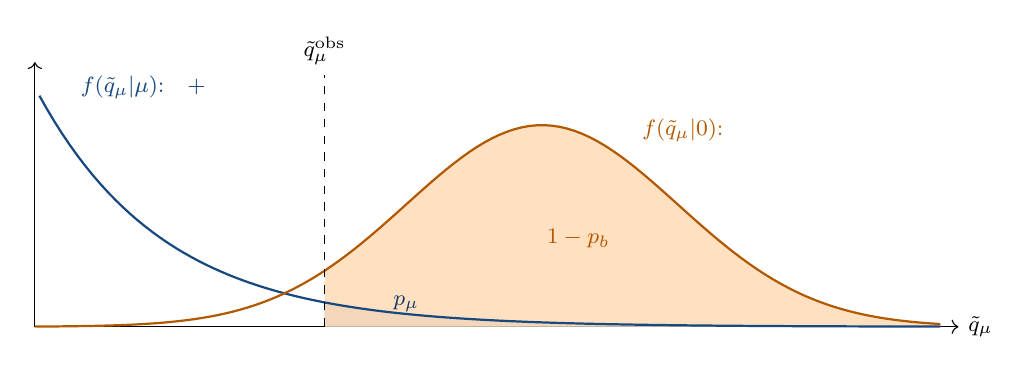
\begin{tikzpicture}[font=\footnotesize, x=1.15cm, y=3.2cm]
\draw[->] (0,0) -- (10.2,0) node[right]{$\tilde q_\mu$};
\draw[->] (0,0) -- (0,1.05);
\fill[accent!25, domain=3.2:10, samples=60] (3.2,0) -- plot (\x,{0.95*exp(-\x/1.4)}) -- (10,0) -- cycle;
\fill[orange!30, opacity=0.8, domain=3.2:10, samples=60] (3.2,0) -- plot (\x,{0.8*exp(-(\x-5.6)^2/(2*1.5^2))}) -- (10,0) -- cycle;
\draw[accent, thick, domain=0.05:10, samples=120] plot (\x,{0.95*exp(-\x/1.4)});
\draw[orange!70!black, thick, domain=0:10, samples=120] plot (\x,{0.8*exp(-(\x-5.6)^2/(2*1.5^2))});
\draw[dashed] (3.2,0) -- (3.2,1.0) node[above]{$\tilde q_\mu^{\mathrm{obs}}$};
\node[accent, anchor=west] at (0.4,0.95) {$f(\tilde q_\mu|\mu)$: 신호+배경};
\node[orange!70!black, anchor=west] at (6.6,0.78) {$f(\tilde q_\mu|0)$: 배경만};
\node[accent!80!black] at (4.1,0.09) {$p_\mu$};
\node[orange!70!black] at (6.0,0.35) {$1-p_b$};
\end{tikzpicture}
\caption{CL\textsubscript{s} 의 개념(모양은 설명용). 오른쪽 꼬리의 넓이가 $p_\mu$(파랑)와 $1-p_b$(주황)다. 두 분포가 많이 겹치면(민감도가 낮으면) $1-p_b$ 도 작아져 CL\textsubscript{s} 가 커진다.}
\label{fig:stats-cls}
\end{figure}

\textbf{점근 공식과 Asimov data}. 표본이 크면 $\tilde q_\mu$ 의 분포를 해석적으로 쓸 수 있고(Cowan–Cranmer–Gross–Vitells), 필요한 것은 $\hat\mu$ 의 표준편차
$\sigma$ 하나다. 이것은 \textbf{Asimov data} — 각 bin 의 관측 수를 어떤 가설(예: $\mu=0$, nuisance 는 사전값)의 기댓값 그대로 둔 가상의 data — 로
구한다: Asimov data 에서는 모든 추정값이 참값과 같으므로 $\sigma^2=\mu^2/\tilde q_{\mu,A}$ 다. 배경만 있는 경우의 중앙값 기대 상한과 그 band 는
\begin{equation}
  \mu_{\mathrm{up}}^{\mathrm{med}}=\sigma\,\Phi^{-1}(1-\alpha/2)\approx1.96\,\sigma,\qquad
  \mu_{\mathrm{up}}^{\pm N}=\sigma\bigl[\Phi^{-1}\bigl(1-\alpha\,\Phi(N)\bigr)+N\bigr],\quad \alpha=0.05,
  \label{eq:stats-expected}
\end{equation}
이다($\Phi$ 는 표준 정규 누적 분포, $N=\pm1,\pm2$ 가 68 \%, 95 \% band). 직관: 계통 없는 단일 계수 실험에서 $s\ll b$ 이면 $\sigma\approx\sqrt{b}/s$ 이므로
$\mu_{\mathrm{up}}\approx1.96\sqrt{b}/s$ 다 — 기대 상한 수십 × SM 은 "유효한" $s/\sqrt{b}$ 가 0.0x 라는 뜻이다(AN SL 의 46.5 는 대략 $s/\sqrt b\approx0.04$; 우리 계산,
통계만의 근사). blind 분석의 "Observed (Asimov)" 는 $\mu=1$ Asimov data 에 fit 한 값이라 구성상 $\hat\mu=1$ 이고, 그 오차가 기대 정밀도다.

\begin{note}[한 bin 으로 해 보기 — 위 식들이 어디서 오나]
bin 하나, $\nu=\mu s+b$, nuisance 없음. $\ln\mathcal{L}(\mu)=n\ln(\mu s+b)-(\mu s+b)$ 이고 최적값은 $\hat\mu=(n-b)/s$ 다.
(1) \textbf{오차}: Fisher 정보 $I(\mu)=-E[\partial^2_\mu\ln\mathcal{L}]=s^2/(\mu s+b)$ 이므로 $\sigma_{\hat\mu}=\sqrt{\mu s+b}/s$, $\mu=0$ 에서 $\sqrt b/s$.
(2) \textbf{Wald 근사}: $-2\ln\lambda(\mu)\approx(\mu-\hat\mu)^2/\sigma^2$. 배경만의 Asimov data($n=b$, $\hat\mu=0$)에서 $\tilde q_{\mu,A}=\mu^2/\sigma^2$ — 식~\eqref{eq:stats-expected} 의
$\sigma^2=\mu^2/\tilde q_{\mu,A}$ 다. 이때 $p_\mu=1-\Phi(\mu/\sigma)$, 중앙값에서 $1-p_b=1/2$ 이므로 $\mathrm{CL_s}=2[1-\Phi(\mu/\sigma)]=0.05$ 에서 $\mu_{\mathrm{up}}=1.96\,\sigma$.
(3) \textbf{기대 유의도}: $\mu=1$ Asimov data($n=s+b$)에서 $q_{0,A}=-2\ln[\mathcal{L}(0)/\mathcal{L}(1)]=2[(s+b)\ln(1+s/b)-s]$, 즉 $Z_A=\sqrt{q_{0,A}}$ —
\ref{ch:mva}장 식~\eqref{eq:mva-za} 에서 $\sigma_b\to0$ 인 경우다. 배경 불확도 $\sigma_b$ 를 nuisance 로 넣고 profile 하면 \eqref{eq:mva-za} 의 전체 꼴이 나온다.
\end{note}

% -----------------------------------------------------------------------------
\section{fit 진단: pull, impact, 적합도}\label{sec:stats-diag}

\begin{itemize}
\item \textbf{pull 과 제약}: fit 뒤 $(\hat\theta_k-0)/1$ 이 pull, 사후 오차 $\sigma_k^{\mathrm{post}}<1$ 이면 data 가 그 nuisance 를 사전보다 강하게 제약한 것이다.
  큰 pull 은 모델이 data 와 어긋난 곳, 강한 제약은 template 이 실제 이상으로 민감하거나(예: 한 과정의 큰 변형) data 가 정보를 가진 곳이다. AN 은 JER 의
  제약이 tt 의 큰 JER 변형에서 온다는 것을 과정별 분리 fit 으로 확인했다\src{AN-22-122 v26, PDF p.126, 164--166}.
\item \textbf{impact}: $\theta_k$ 를 $\hat\theta_k\pm\sigma_k^{\mathrm{post}}$ 에 고정하고 다시 fit 했을 때 $\hat\mu$ 가 움직이는 양 $\Delta\hat\mu$. 큰 순서로 늘어놓아 결과를
  지배하는 불확도를 찾는다. 자유 정규화도 같은 방식으로 순위에 오른다("Unconstrained").
\item \textbf{적합도(GoF)}: saturated 모델 검정은 $-2\ln[\mathcal{L}(\hat\mu,\hat{\vec\theta})/\mathcal{L}_{\mathrm{sat}}]$ ($\mathcal{L}_{\mathrm{sat}}$ 는 bin 마다
  $\nu_i=n_i$)를 toy 의 분포와 비교한다. KS·AD 검정도 쓴다. ttH 는 \texttt{combine -M GoodnessOfFit -{}-algo "saturated"} 를 썼다\src{AN-19-094 v20, PDF p.158}.
\item \textbf{배경 bin 만의 fit}: blind 일 때 신호가 적은 bin 으로만 fit 해 모델이 data 를 설명하는지 본다(AN Fig.~98\src{AN-22-122 v26, PDF p.126}).
\end{itemize}

\textbf{combine}. CMS 의 통계 도구 combine 은 datacard(채널별 관측 수, 과정별 기댓값과 template, \code{lnN}·\code{shape} nuisance, \code{rateParam},
\texttt{autoMCStats})를 읽어 식~\eqref{eq:stats-L} 을 만든다. AN SL 은 combine v8.2.0(CMSSW\_10\_6\_29)으로 기대 상한과 Asimov 최적값을 구했다\src{AN-22-122 v26, PDF p.119}:
{\small
\begin{verbatim}
combine -M AsymptoticLimits card.root -m 125 --run blind --rMin=-40 --rMax=40
combine -M FitDiagnostics --saveWithUncertainties --saveShapes --rMin=-40 --rMax=40 -m 125 card.root
\end{verbatim}
}
\texttt{-{}-run blind} 은 data 를 보지 않고 배경만의 Asimov data 로 기대 상한만 낸다.

% -----------------------------------------------------------------------------
\section{Run 2 AN(ttHH SL·DL)의 설정과 결과}\label{sec:stats-an}

\textbf{설정}. SL 은 연도별로 4 개 fit node(ttHH, ttH, ttZ(1 bin), ttbar; \ref{ch:mva}장)의 판별 변수를 binned shape fit 한다("5j4b model option 2"),
자유 정규화는 \code{mu_ttbar}, \code{mu_ttH}($[-5,5]$)\src{AN-22-122 v26, PDF p.119, 123}. DL 은 6 node 판별 변수의 동시 binned ML fit 으로, 일부 nuisance 에
log-normal 사전 분포, shape 변형은 연속 template morphing 이다\src{AN-22-122 v26, PDF p.131}. 결과는 모두 Asimov(blind)이고 실 data 결과의 §9 는
제목만 있다\src{AN-22-122 v26, PDF p.138}.

\begin{table}[htbp]
\centering
\caption{AN-2022/122 의 기대 95 \% CL 상한($\mu$, Asimov). [68 \%] [95 \%] 는 band. PDF 쪽: SL Table 54--57 p.126--127, DL Table 59--66 p.132--133, 결합 Table 67 p.137.}
\label{tab:stats-an}
\small
\begin{tabular}{@{}llrl r@{}}
\toprule
채널 & 데이터 & stat+syst & [68 \%] [95 \%] & stat 만 \\
\midrule
SL(5j4b) & 2016 & 95.7 & [65.8, 143.5] [47.9, 210.9] & 89.3 \\
 & 2017 & 76.3 & [52.4, 114.5] [38.1, 168.2] & 71.5 \\
 & 2018 & 63.5 & [43.7, 94.4] [32.2, 138.0] & 58.5 \\
 & Run 2 & \textbf{46.5} & [32.2, 68.9] [23.6, 100.4] & 39.0 \\
\midrule
DL & 2016 & 91.75 & [57.59, 151.00] [39.07, 237.00] & 88.25 \\
 & 2017 & 71.88 & [45.66, 116.00] [31.45, 180.90] & 69.88 \\
 & 2018 & 60.00 & [38.23, 96.83] [26.02, 150.34] & 58.00 \\
 & Run 2 & \textbf{34.63} & [22.49, 54.50] [15.69, 82.67] & 28.63 \\
\midrule
SL+DL & Run 2 & \textbf{25.13} & [17.05, 37.44] [12.37, 54.03] & — \\
\bottomrule
\end{tabular}
\end{table}

SL Run 2 의 Asimov 최적값은 $1.0^{+22.1}_{-21.0}$(통계만 $^{+19.5}_{-18.5}$), 결합은 $1.0^{+11.68}_{-7.96}$ 이다\src{AN-22-122 v26, PDF p.127, 137}. AN 은 "DL 의 민감도가
SL 과 비슷하다 — ttH 와 일관" 이라 쓴다\src{AN-22-122 v26, PDF p.137}. HEFT 해석(SL 만)은 $\sigma_{\ttHH}(\kl,\kt,c_2)$ 를 여섯 항의 다항식으로 매개화하고
기대 95 \% CL $-5.0<c_2<4.8$ 를 얻었다\src{AN-22-122 v26, PDF p.127, Eq.~22}.

\textbf{발표의 최신 숫자}. SL 승인 발표의 최종 fit(tt 와 ttb 분리, ttH·ttbar·ttb 자유)은 Run 2(137.6\fbinv) 기대 상한 \textbf{55.3 × SM}, 관측
\textbf{48.7 × SM}, 즉 $\sigma(\ttHH)$ 에 관측(기대) 37(42)\fb 다\src{승인 발표 p.33}\src{Wei Wei, DPF 2026 p.12}. 최적값은 $-8.9^{+25.8}_{-24.8}$(그림 판독)
\src{승인 발표 p.32}. 2025-12-02 의 둘째 ARC 회의에서 쓴 tt 병합 모델은 기대 50.5, 관측 79.3, 최적값 29.0 이었고, ARC 와 "나누는 것이 낫다" 고
합의했다(그림 판독)\src{승인 발표 p.29--32}. 37(42)\fb 는 $\sigma_{\mathrm{SM}}=0.756\fb$ 로 환산한 값과 맞는다($48.7\times0.756=36.8$, $55.3\times0.756=41.8$;
우리 계산). HEFT 의 관측(기대)은 $-6.6<c_2<6.4$($-5.4<c_2<5.2$)다\src{승인 발표 p.35}. 사전승인 발표(2025-04)의 SL+DL 기대 상한은 25.13 × SM 이었다
\src{사전승인 발표 p.26}. 관측·기대 유의도와 $\kl$ 단독 제약은 어느 자료에도 없다.

\begin{openq}[숫자가 서로 다른 곳]
AN v26 Table 57 의 SL Run 2 기대 상한은 46.5 인데, 사전승인 발표 p.25 의 표(그림)에는 SL 42.5 로 읽힌다(발표 digest 판독). 그런데 SL+DL 결합 25.13 은 두 자료에서
같다 — AN 의 결합 표가 SL 의 갱신 뒤에 다시 계산되었는지 확인할 수 없다. 승인의 최종 SL 기대 55.3 은 fit 모델(tt/ttb 분리)이 달라 직접 비교할 수 없다.
\end{openq}

% -----------------------------------------------------------------------------
\section{참고: ttH(bb) FH 의 fit — 자유 QCD 정규화}\label{sec:stats-tth}

ttH(bb) FH 는 ANN 출력(\code{DNN_Node0})을 범주 3 개(7, 8, $\ge9$ jet; $\ge4$ b) × 3 년으로 fit 한다. bin 은 20 개 균등에서 시작해 빈 bin 을 합친 뒤
절반으로 줄인 "Option 2" 다\src{AN-19-094 v20, PDF p.115--117}. QCD 는 CR 에서 만든 template(\ref{ch:qcd}장)이고 정규화는 연도 × 범주 9 개가 사전 제약
없이 자유다. FH 단독 fit 에서는 tt+B, tt+C 정규화를 50 \% lnN 으로 묶는다\src{AN-19-094 v20, PDF p.243}. 결과는 표~\ref{tab:stats-tth}.

\begin{table}[htbp]
\centering
\caption{ttH(bb) FH 단독 fit(AN-19-094 v20, Table 128--132, PDF p.223, 243--246).}
\label{tab:stats-tth}
\small
\begin{tabular}{@{}lllll@{}}
\toprule
 & Run 2 & 2016 & 2017 & 2018 \\
\midrule
Asimov $\mu$ & $1.00^{+0.77}_{-0.78}$(stat $\pm0.23$), 1.3$\sigma$ & $^{+1.09}_{-1.14}$ & $^{+1.26}_{-1.37}$ & $^{+1.12}_{-1.21}$ \\
관측 $\mu$ & $-1.31^{+0.82}_{-0.89}$(stat $\pm0.20$) & $0.91^{+1.17}_{-1.22}$ & $-1.44^{+1.51}_{-1.63}$ & $-2.44^{+1.37}_{-1.58}$ \\
saturated GoF $p$ & 0.46 & 0.84 & 0.34 & 0.45 \\
\bottomrule
\end{tabular}
\end{table}

자유 QCD 정규화는 FH 단독 data fit 에서 0.912--0.974 로, 범주마다 $\pm$1.3--3.5 \% 의 정밀도로 정해졌다\src{AN-19-094 v20, PDF p.237, Fig.~128}. 사전 제약이
없어도 SR 자체가 QCD 를 잡는 이유는 QCD 가 SR 의 대부분이고(ttH FH SR 에서 67--83 \%) 판별 변수의 낮은 점수 bin 이 사실상 QCD 의 control
region 역할을 하기 때문이다\src{PLAN\_QCD\_DD §1}. 채널 사이 nuisance 를 상관시킨 다중 POI fit 에서 FH 는 $0.84^{+0.49}_{-0.46}$ 로, FH 단독(−1.31)과 크게
다르다\src{AN-19-094 v20, PDF p.244, Fig.~135}. 상관 fit 에서는 tt+B·tt+C 정규화도 50 \% lnN 대신 다른 채널과 공유하는 자유 정규화가 된다
\src{AN-19-094 v20, PDF p.243} — 그 처리(와 다른 nuisance 의 공유)가 FH 결과를 크게 바꾼다는 뜻으로 읽는다(우리 판단).

\begin{note}[ttHH FH 에 주는 시사점(우리 판단)]
(1) ttHH 의 SR 통계는 ttH 보다 훨씬 적어, SR 만으로는 자유 QCD 정규화가 덜 고정될 수 있다 — 정규화를 연도나 범주 사이에 공유하거나 CR 을 fit 에 넣는
설계를 검토한다\src{PLAN\_QCD\_DD §5}. (2) FH 단독은 tt+B 에 약하므로 단독 결과는 tt+B 처리에 민감하다 — SL/DL 과의 결합에서 tt+B 를 공유하는 것이 자연스럽다.
(3) DNN 의 QCD node 와 배경 node 는 fit 안의 control region 이다.
\end{note}

% -----------------------------------------------------------------------------
\section{우리 FH fit 계획}\label{sec:stats-ours}

모두 \tagplan 이고 결정 전이다. 순서는 \textbf{FH 단독 fit} 이 먼저이고(SL/DL 과의 결합은 그 뒤), 그 안에서 2024 단독 → Run 2 → Run 2 + 2024 다.

\textbf{영역과 범주}. 사용자 Hbb 발표의 출발점은 SR = $n_b\ge4$, jet 범주 7 / 8 / $\ge9$, Higgs 후보 질량창(예: 100--140\GeV)이다\src{Hbb 회의 FH 발표 p.14}.
ttHH 는 b quark 6 개라 $n_M\ge5$ 나 ($n_M=4$, $n_M\ge5$) 범주가 더 민감할 수 있어, QCD 영역을 SR($n_M\ge N$), CR($n_M=N-1$, $n_L\ge N$), TR($n_M=N-2$, $n_L\ge N$)로
일반화해 두었다\src{PLAN\_QCD\_DD §3.1}(그림~\ref{fig:stats-regions}). 범주와 질량창은 SR 최적화(ROADMAP W5)에서 정한다.

\begin{figure}[htbp]
\centering
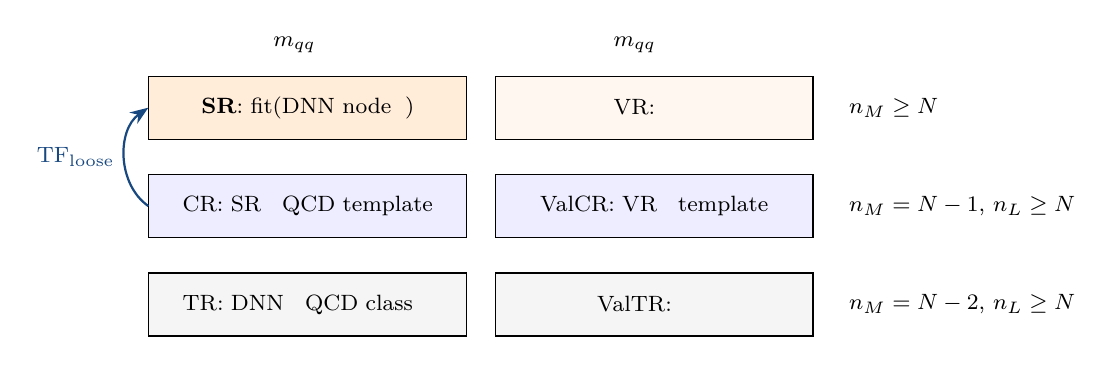
\begin{tikzpicture}[font=\footnotesize, x=1cm, y=1cm, >=Stealth]
\tikzset{reg/.style={draw, text width=38mm, minimum height=8mm, align=center}}
\node[reg, fill=orange!15] (sr)  at (0,2.5)    {\textbf{SR}: fit(DNN node 별)};
\node[reg, fill=orange!6]  (vr)  at (4.4,2.5)  {VR: 추정 검증};
\node[reg, fill=blue!7]    (cr)  at (0,1.25)   {CR: SR 의 QCD template};
\node[reg, fill=blue!7]    (vcr) at (4.4,1.25) {ValCR: VR 의 template};
\node[reg, fill=black!4]   (tr)  at (0,0)      {TR: DNN 의 QCD class 학습};
\node[reg, fill=black!4]   (vtr) at (4.4,0)    {ValTR: 입력 검증};
\node at (0,3.3)   {$m_{qq}$ 중앙창};
\node at (4.4,3.3) {$m_{qq}$ 사이드밴드};
\node[anchor=west] at (6.75,2.5)  {$n_M\ge N$};
\node[anchor=west] at (6.75,1.25) {$n_M=N-1$, $n_L\ge N$};
\node[anchor=west] at (6.75,0)    {$n_M=N-2$, $n_L\ge N$};
\draw[->, thick, accent] (cr.west) to[bend left=55] node[left]{TF\textsubscript{loose}} (sr.west);
\end{tikzpicture}
\caption{QCD 추정과 fit 의 영역(ttH(bb) FH 방식을 $N$ 으로 일반화; ttH 는 $N=4$). $n_M$, $n_L$ 은 M, L 을 넘는 jet 수, $m_{qq}$ 는 \texttt{invMassHadW}. 각 영역은 jet 범주마다 따로.}
\label{fig:stats-regions}
\end{figure}

\textbf{판별 변수}. \ref{ch:mva}장의 다중 분류 DNN 으로 event 를 최대 node 에 보내고, node 마다 그 node 점수 분포를 template 으로 쓴다. fit node 는 ttHH, ttH, ttZ,
tt(lf+cc), ttb(mb+nb), QCD 가 후보다(AN 의 node 병합과 승인의 tt/ttb 분리; \ref{ch:mva}장 표~\ref{tab:mva-classes}). binning 은 AN 이 적지 않았으므로
(DL 의 ttHH node 는 impact 이름에 \code{bin0}–\code{bin9} 가 보여 10 bin 으로 보인다\src{AN-22-122 v26, PDF p.135, Fig.~105}) ttH FH 의 방식(균등 bin 에서
빈 bin 병합 후 축소)과 MC 통계로 정한다.

\textbf{자유 parameter 와 nuisance}. QCD 정규화(연도 × 범주, 자유), tt·ttb 정규화(자유 또는 50 \% lnN — \ref{ch:syst}장 미결), ttH 정규화(AN 처럼 자유 또는
단면적 불확도). 나머지는 \ref{ch:syst}장의 표.

\textbf{Run 2 + 2024 결합}. 채널을 era(2016preVFP, 2016postVFP, 2017, 2018, 2024)마다 두고 공통 $\mu$ 하나를 둔다. $\mu$ 는 각 $\sqrt{s}$(13, 13.6\TeV)의 SM
단면적에 대한 비이므로, 결합은 "두 에너지에서 같은 비" 를 가정한다. 상관 방식은 \ref{ch:syst}장 표~\ref{tab:syst-corr} 의 제안이다 \tagopen. 첫 결과는
2024 단독(표본이 모두 있음), 다음이 Run 2(v15 신호 표본을 기다림)다\src{ROADMAP\_FH §1, §6}.

\textbf{blinding}. preselection 과 control region 의 plot 에는 data 를 모두 보이고, 최종 판별 변수에서 기대 S/B 가 큰 bin(예: $\ge4$ b 범주의 높은 DNN 점수)만
가린다. 기준과 unblinding 절차는 AN 에서 가져온다\src{D-2026-10-02-E}. preselection 에서 신호는 2017(42.07\fbinv)에 약 11 event, 2024 C--I 에 약 28 event 만
생성되어(선택 전) data 로 신호를 볼 수 없기 때문이다\src{D-2026-10-02-E}. AN 도 data 를 신호가 적은 bin 에만 그렸다\src{AN-22-122 v26, PDF p.112}.
절차(제안): (1) Asimov 기대 결과와 impact, (2) 가린 bin 을 뺀 data fit 과 GoF, pull 확인, (3) 검토 뒤 unblinding.

\textbf{SL/DL 과의 결합}. FH 는 lepton veto 로 SL·DL 과 겹치지 않도록 정의되고, 결합은 "채널들이 양립 가능하다고 판명되면" 할 수 있다\src{Hbb 회의 FH 발표 p.38}.
결합에서는 b-tag, JES, 이론, tt+B 의 nuisance 를 채널 사이에 맞춰야 한다. 문서 경로(같은 AN 의 보완 채널 대 후속 결과)는 팀 확인이 필요하다
\src{Hbb 회의 FH 발표 p.5}\src{KCMS 발표 p.4}.

% -----------------------------------------------------------------------------
\section{미결 사항}\label{sec:stats-open}

\begin{openq}
\begin{enumerate}
\item \textbf{SR 정의}: $N$($n_M\ge4$ 대 $\ge5$), jet 범주, Higgs 질량창; 범주 수와 자유 QCD 정규화의 개수(공유할지, CR 을 fit 에 넣을지).
\item \textbf{fit node 와 binning}: tt/ttb 분리(승인 모델)를 따를지, QCD node 의 역할, bin 경계를 정하는 규칙.
\item \textbf{tt+B 처리}: FH 단독 결과에서 50 \% lnN 대 자유.
\item \textbf{Run 2 + 2024 결합}: 공통 $\mu$ 의 정의, nuisance 상관(\ref{ch:syst}장), Run 2 v15 신호 표본이 없을 때의 순서.
\item \textbf{blinding 기준}: "기대 S/B 가 큰 bin" 의 수치 기준과 unblinding 절차(AN 에서 가져올 것).
\item \textbf{결합과 문서}: SL/DL(HIG-24-016)과의 결합 시점과 방식, 같은 AN 인지 별도 결과인지(팀 확인).
\item \textbf{숫자 확인}: AN v26 의 SL 46.5 대 사전승인 42.5(위 상자).
\end{enumerate}
\end{openq}

% =============================================================================
% 12 장 — 현재 상태
% =============================================================================
\chapter{현재 상태}\label{ch:status}

이 장은 2026-10-10 기준으로 분석의 각 부분이 어디까지 왔는지를 한 번에 보여 준다. 앞 장들이 ``무엇을 왜''를 다뤘다면 여기서는
``지금 어디''를 다룬다. 연도별·단계별 상태표(\ref{sec:status-table}절), 코드가 바뀌어 온 흐름(\ref{sec:status-history}절), 시험 상태
(\ref{sec:status-tests}절), 그리고 이 문서를 쓰면서 드러난 분석의 문제(\ref{sec:status-findings}절)를 차례로 적는다. 날마다의 상세는
\file{docs/STATUS.md} 가 정본이다.

\section{한눈에 보기}\label{sec:status-table}

\begin{table}[htbp]\centering
\caption{단계별·연도별 상태(2026-10-10). 2016 은 두 반쪽(preVFP, postVFP) 모두 아직 v15 ntuple 이 없어 표에서 뺐다.}\label{tab:status-overview}
\small
\begin{tabularx}{\linewidth}{@{}>{\raggedright\arraybackslash}p{2.6cm} L L L@{}}
\toprule
단계 & 2017(Run 2) & 2018(Run 2) & 2024(Run 3) \\
\midrule
ntuple\newline(NtupleForge) & v20(NanoAOD v9) 생산본은 KNU 에서 지워짐\src{D-2026-10-05-D}; v15 재생산 전 & v15 생산 끝 & v15 생산 끝(MC, JetMET, ParkingHH)\src{STATUS 10-07} \\
analyzer & v9 이름으로 동작(2017 회귀 기준 Y1) \tagtest & v15 이름 미지원 — 필수 branch 검사에서 의도된 FATAL; 할 일 A–K\src{ROADMAP\_FH §3} \tagplan & 동작(STEP 24–27) \tagtest \\
lumi(\fbinv) & 42.07\src{LUMI\_SOURCES §2} & 59.56(brilcalc 미실행)\src{LUMI\_SOURCES §2} & 109.816(C–I)\src{LUMI\_SOURCES §6} \\
trigger SF & 유도본이 KNU 에만 있음(STEP 26 이전 판) & 기준 trigger 미결(\ref{ch:trigger}장) \tagopen & 도구 준비(STEP 26) \tagtest; btagtrig 출력 대기 \\
b-tag SF & shape SF + norm reweight(저장소의 JSON 은 옛 7묶음 판; main 은 norm reweight 끔 — tt+nb 키 판 미재생성)\src{2017 main 의 yml} & payload 준비 전 & fixed-WP method 1a(STEP 25, 27) \tagtest; 효율 map 은 btagtrig 뒤 \\
stitching & JSON 있음, main 에는 꺼짐; 정규화 문제(\ref{sec:status-findings}절) \tagopen & — & 꺼짐(tt+nb lookup 없음)\src{D-2026-10-05-C} \\
control plot & Hbb 회의 FH 발표(2026-07-30) & — & SF 없는 FH·μCR·eCR\src{STATUS 10-09 (3)}; SF 판 대기 \\
Tree v1(ML 입력) & 코드 공통 \tagtest & 코드 공통 & 코드·시험 끝, KNU 실행 전\src{STEP 27} \\
QCD data-driven & \multicolumn{3}{>{\raggedright\arraybackslash}p{12.8cm}}{계획(\ref{ch:qcd}장) \tagplan; lepton CR 의 Data/MC 가 맞은 뒤\src{D-2026-10-10-B}} \\
DNN·GATJA & \multicolumn{3}{>{\raggedright\arraybackslash}p{12.8cm}}{설계(\ref{ch:mva}장) \tagplan; Run 2 v15 의 신호 표본 부재가 Run 2 학습을 막음} \\
계통·fit & \multicolumn{3}{>{\raggedright\arraybackslash}p{12.8cm}}{weight 변형은 Tree 에 기록 \tagimpl; JES/JER 변형 미구현; fit 은 계획 \tagplan} \\
\bottomrule
\end{tabularx}
\end{table}

\paragraph{지금의 임계 경로.} 2024 의 SF 를 넣은 control plot 이다: btagtrig 완료 $\to$ merge $\to$ b-tag 효율 map $\to$ TriggerStudy(2024 trigger SF)
$\to$ STEP 27 실행 파일로 SF main 셋(FH, μCR, eCR) $\to$ plot\src{ROADMAP\_FH, 결론 먼저}. 그 SF main 을 Tree v1 이 든 실행 파일로 돌리면
control plot, DNN 입력 변수의 Data/MC, 첫 학습 표본이 한 번에 나온다. 2026-10-10 KNU 에서는 2024 btagtrig job(6,353 개)이
\code{request_memory} 12\,GB 때문에 거의 돌지 못하는 것이 확인됐고(analyzer job 의 실측 최대 286\,MB), 제출기의 기본값은 STEP 27 에서
2\,GB 로 바꿨다\src{STATUS 10-10}.

\paragraph{결과까지 막는 외부 의존.} (a) Run 2 v15 에 신호(\texttt{TTHHTo4b})와 \texttt{TT4b}, \texttt{TTZHTo4b}, \texttt{TTZZTo4b}, \texttt{THW} 가
중앙 생산에 없다 — 요청은 2026-09-14 에 했고, enriched 사설 생산을 병행한다. (b) 2016·2017 v15 hadronic ntuple 생산 전. (c) 2024 의
W$\to\ell\nu$·DY 표본(lepton CR 의 MC 합)과 tt+nb patch(2024 stitching)\src{ROADMAP\_FH, 결론 먼저; D-2026-10-10-B}.

\section{지금까지의 흐름}\label{sec:status-history}

코드의 변경은 STEP 단위로 기록한다(\file{docs/changes/STEP_*.md}). 각 기록에는 무엇을, 왜, 원래 형태, 되돌리는 법, 검증이 있다\src{docs/changes/README}.

\begin{table}[htbp]\centering
\caption{변경의 큰 흐름. 날짜는 각 STEP 문서의 첫 날짜다.}\label{tab:status-steps}
\small
\begin{tabularx}{\linewidth}{@{}l l L@{}}
\toprule
시기 & STEP & 내용 \\
\midrule
2026-06-11–12 & 0–9 & 리팩토링: 변경 기록 체계, stitchWeight branch, debug mode, 선언적 cut 표(\texttt{kCutSequence}), 경로의 yml 화, event-shape 라이브러리, HiggsReconstructor(HH/ZH/ZZ), condor 개선, 8 묶음 카테고리, 주석 정리, README \\
2026-06-12–15 & 10–16 & ttbb weight, cross section 단일 출처(xsec\_db), fb 단위와 AN 기반 $\sigma$/BR 수정, 3 단계 weight(trigSF / +btagShape / +normRW), lepton CR(1$\ell$+MET), region 출력 분리, SF 토글 \\
2026-06-29–07-12 & 17–22 & fullNano v20 dataset 과 genTtbarId 표준 디코드, NtupleForge 표본 이름, 완료 표지, report 표, plotter 전 표본, merge 자동 탐색 \\
2026-10-04 & 23 & KNU 의 긴 단계를 condor job 으로, 실행 기록(\texttt{runlogs/})을 커밋 \\
2026-10-05–07 & 24 & 2024 analyzer: EraConfig 2024, v15 이름, 필수 branch 검사, PU, jet veto map, PD 규칙(ParkingHH) \\
2026-10-08 & 25 & 2024 fixed-WP b-tag weight(method 1a), 효율 map 도구\src{D-2026-10-08-A} \\
2026-10-09 & 26 & TriggerStudy 의 2024, trigger SF JSON 의 연도 검사, merge guard \\
2026-10-10 & 27 & BTV 다중 WP 규칙(\src{D-2026-10-10-A}), Tree v1(ML 입력, jet 정답 표지, 계통 weight), 제출기 \texttt{--memory} 2\,GB \\
2026-10-10 & 27 P & 독립 검토 반영: jet 의 top 표지(\texttt{jetGenTopIdx}), \texttt{--tree-v1 on|off}, Run 2 shape 키의 load 검사(E40), 병합 전 \texttt{Tree/Tree} branch 집합 검사(exit 8) \\
\bottomrule
\end{tabularx}
\end{table}

큰 방향의 결정은 다음 순서로 내려졌다: 2024 를 v15 의 첫 대상으로(D-2026-10-02-A), blinding 은 최종 판별변수의 신호 민감 bin 만(D-2026-10-02-E),
2024 첫 plot 은 SF 없이(D-2026-10-05-A), 2024 의 b-tag 경로는 ParkingHH(D-2026-10-06-A), 2024 lepton CR 먼저(D-2026-10-07-B),
2024 b-tag 은 fixed WP(D-2026-10-08-A)와 BTV 다중 WP 규칙(D-2026-10-10-A), 그리고 FH 전체의 방향(D-2026-10-10-B)\src{DECISIONS}.

\section{시험 상태}\label{sec:status-tests}

STEP 27 의 컨테이너 시험: 단위 시험 \texttt{test\_TreeVars} 27/27, offline smoke 110/110(그중 15 개가 새 것), failure checks 76/76,
runlog 85/85\src{STEP 27; STATUS 10-10 (2)}. 독립 검토(코드 리뷰 에이전트)는 BUG 0, RISK 4 를 냈고, 그것을 반영한 STEP 27 P 뒤에는 단위 30/30,
offline smoke 116/116, failure checks 81/81 이다\src{STEP 27 §P}. KNU 에서는 10-09 에 2024 smoke 106/106\src{STEP 26 §10}. 2017 은 새 코드가 옛 실행 파일과
같은 출력을 내는지(Y1 비교)를 합성 입력으로 확인했다\src{STEP 27}. 실제 2017 파일로의 Y1 은 v20 ntuple 이 지워져 지금은 할 수 없다\src{D-2026-10-05-D}.

\section{이번 판에서 찾은 문제}\label{sec:status-findings}

이 문서를 쓰며 원문·발표·코드를 맞대어 보다가 분석 자체의 문제가 드러났다. 아래는 결정이 필요한 것들이며, 자세한 설명은 괄호 안의 장에 있다.

\begin{enumerate}[leftmargin=*]
\item \textbf{stitching 정규화에 $p_{\text{own}}$ 이 빠져 있다}(\ref{ch:samples}장) \tagopen.
\code{compute_stitch_factors.py} 의 $r=\sigma_{\text{inc}} f/\sigma_{\text{ded}}$ 는 dedicated 표본 \textbf{전체}를 inclusive 의 소유 칸 단면적
$\sigma_{\text{inc}}f$ 로 맞춘 뒤 소유 칸만 남긴다. 그러면 소유 칸의 수율은
\begin{equation}
N_{\text{owned}} = L\,\sigma_{\text{inc}}\,f\,p_{\text{own}},\qquad p_{\text{own}}=\frac{\sum_{\text{ded, owned}} g}{\sum_{\text{ded, all}} g}
\label{eq:status-pown}
\end{equation}
이 되어 목표 $L\sigma_{\text{inc}}f$ 보다 $p_{\text{own}}$ 배 작다. 2017 prescan 에서 4FS ttbb 표본의 53–55 비율은 Had 0.114, SL 0.108,
DL 0.103 이다\src{prescan\_summary.json(2017), genTtbarId sumGenW}. 즉 stitched tt+bb 는 목표의 약 1/9 이다. 지금은 어떤 main 도 stitching 을
쓰지 않아(2017 main 과 2024 의 \texttt{path\_stitch\_json} 이 null) 기존 plot 은 영향이 없고, 2017 btagtrig 의 norm reweight 유도만
그 JSON 을 읽는다. 고치는 식 $r'=r/p_{\text{own}}$ 과 closure 시험을 \src{D-2026-10-10-C}(PROPOSED)에 적었다.
\item \textbf{tt+b, tt+2b(genTtbarId 51, 52)의 소유가 AN 과 다르다}(\ref{ch:samples}장) \tagopen. 우리 EXP 는 5FS 에 두고, AN 은 4FS
ttbb 에서 가져온다\src{AN-22-122 v26, PDF p.187, 195, 203}. \ttH(\bbbar) FH 와 우리 Hbb 회의 발표도 4FS 다\src{AN-19-094 v20, PDF p.89; Hbb 회의 FH 발표 p.21}.
\item \textbf{veto muon 의 isolation 이 0.15}다\src{SelectionCuts.h, muonIso}. AN DL 의 부 lepton 과 \ttH(\bbbar) FH 의 veto 는 0.25 이므로
SL/DL 과의 직교성을 결합 전에 확인해야 한다(\ref{ch:objects}장) \tagopen.
\item \textbf{jet–lepton $\Delta R$ cleaning 이 코드에 없다}(\ref{ch:objects}·\ref{ch:selection}장) \tagopen. FH 영역에서는 lepton veto 가 있어 문제가
작지만, lepton CR 에서는 lepton 이 jet 으로도 세어질 수 있다. TightLepVeto jet ID 가 일부만 막는다.
\item \textbf{$\chi^2$ 의 분모}는 $\sqrt{0.1\sum\pt}$ 로 단위가 $\sqrt{\mathrm{GeV}}$ 다\src{HiggsReconstructor.h; STEP 6}. AN 은 JER 로 정한 $\sigma$ 라고만
적었다(숫자 없음)\src{AN-22-122 v26, PDF p.49}. DNN 입력으로 쓰기 전에 정한다(\ref{ch:reco}장) \tagopen.
\item 2016 PU jet ID 의 WP(우리 \texttt{puId}$\geq4$, AN \texttt{puId}$==1$)\src{AN-22-122 v26, PDF p.44}, trigger SF 불확도가 bin 전체가 함께 움직이는
nuisance 하나라는 점(\ref{ch:objects}·\ref{ch:trigger}·\ref{ch:syst}장) \tagopen.
\item 13\TeV{} 신호 단면적이 자료마다 0.756\fb\src{AN-22-122 v26, PDF p.23, Table 9}와 0.775\fb\src{승인 발표 p.3, p.27}로 다르고,
13.6\TeV{} 값 0.860\fb{} 는 임시값이다\src{STEP 24 §7}(\ref{ch:intro}장) \tagopen.
\item 문서 고침: plotter \code{--tree-v1} 의 plot 수는 31 개다(STEP 27 기록과 CHANGELOG 의 32 는 잘못이었고 고쳤다).
\end{enumerate}

AN 원문 안의 불일치(표와 본문이 다른 곳)는 각 장의 \texttt{openq} 상자에 모았다. 우리가 그것을 그대로 따라 하지 않도록 하기 위함이다.

% =============================================================================
% 13 장 — 앞으로의 계획
% =============================================================================
\chapter{앞으로의 계획}\label{ch:plan}

결과(FH 채널의 신호 세기 상한, Run 2 전체 + 2024)까지의 작업을 여덟 갈래(워크스트림 W1–W8)로 나누고, 순서와 의존성, 결정을 기다리는 것,
위험을 적는다. 정본은 \file{docs/ROADMAP_FH.md} 이고, 이 장은 그것을 분석의 흐름 위에 놓고 읽기 위한 요약이다\src{ROADMAP\_FH}.

\section{목표와 일정}\label{sec:plan-goal}

목표는 \ttHH(\HHfourb) FH 채널의 신호 세기 상한이다. Run 2 전체(2016preVFP, 2016postVFP, 2017, 2018)와 2024 를 쓴다. HEFT 해석은
SL 처럼 나중에 한다. SL/DL 과의 결합은 채널들이 양립 가능하면 한다\src{Hbb 회의 FH 발표 p.38}. 일정은 2026 하반기에 full Run 2 로 넓히고
QCD data-driven 방법을 세우고 검증하는 것, 2027 상반기에 다중 분류 DNN, SR 최적화, 계통 불확도를 거쳐 fit 에 이르는 것이다\src{KCMS 발표 p.4}.

\section{워크스트림}\label{sec:plan-ws}

\begin{table}[htbp]\centering
\caption{워크스트림(2026-10-10)\src{ROADMAP\_FH §2}}\label{tab:plan-ws}
\footnotesize
\begin{tabularx}{\linewidth}{@{}l >{\raggedright\arraybackslash}p{2.9cm} L L >{\raggedright\arraybackslash}p{2.0cm}@{}}
\toprule
W & 무엇 & 지금 & 다음 & 이 문서 \\
\midrule
W1 & control plot(SF 적용) & 2024 btagtrig 실행 중, SF 없는 plot 있음 & btagtrig $\to$ 효율 map $\to$ TriggerStudy $\to$ STEP 27 빌드 $\to$ SF main 셋 $\to$ plot(\texttt{--tree-v1} 포함) & \ref{ch:trigger}, \ref{ch:btag}, \ref{ch:selection}장 \\
W2 & analyzer 의 Run 2 v15 & Run 2 는 v9 이름만 & 할 일 A–K(스키마 선택, 이름, jet ID 재계산, PU ID, trigger, PD, payload, lumi, xsec·prescan·stitch, tt+nb, trigger SF·b-tag norm), 2018 먼저 & \ref{ch:objects}, \ref{ch:trigger}장 \\
W3 & 표본(NtupleForge) & 2018 v15·2024 v15·ParkingHH 끝 & 2016·2017 v15 생산, Run 2 부재 5 종, 2024 lepton 표본, 2024 tt+nb patch & \ref{ch:samples}장 \\
W4 & Tree·ML 입력 & Tree v1 코드·시험 끝 & SF main 으로 표본, 내보내기 도구(\texttt{tools/ml/}) & \ref{ch:reco}장, 부록 \ref{ch:treev1} \\
W5 & ML & 설계 & 2024 표본으로 기준선 DNN, GATJA 의 FH 판 & \ref{ch:mva}장 \\
W6 & 계통·통계 & weight 변형의 Tree 기록 & MC 통계 band, JES/JER 변형 실행 경로, datacard & \ref{ch:syst}, \ref{ch:stats}장 \\
W7 & QCD data-driven & 계획 & lepton CR Data/MC 확인 $\to$ 영역 수율 표 $\to$ TF 유도 도구 & \ref{ch:qcd}장 \\
W8 & 한국어 AN & v0.1 & 각 단계가 끝날 때마다 해당 장 & 이 문서 \\
\bottomrule
\end{tabularx}
\end{table}

\section{순서와 의존성}\label{sec:plan-order}

\begin{figure}[htbp]\centering
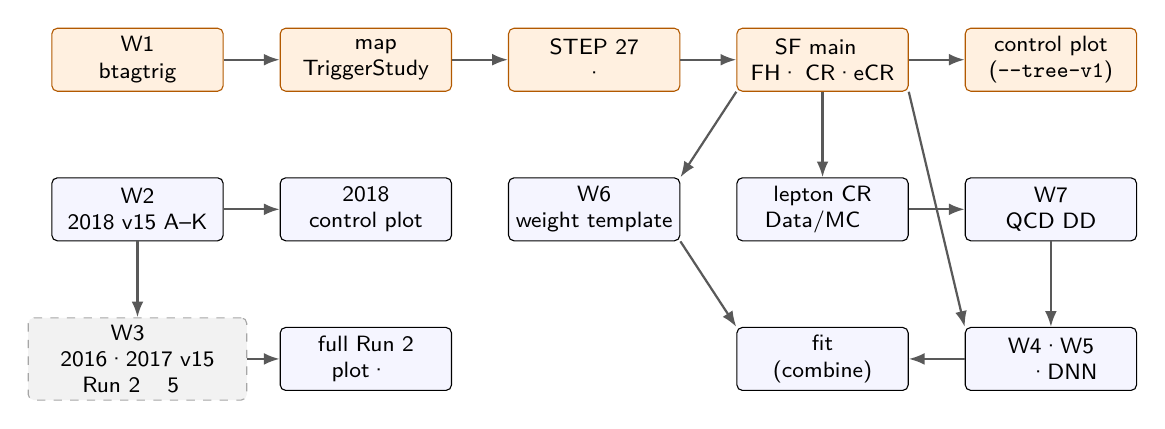
\begin{tikzpicture}[
  box/.style={draw,rounded corners=2pt,fill=blue!4,align=center,font=\footnotesize\sffamily,inner sep=2.5pt,
              text width=2.0cm,minimum height=8mm},
  now/.style={box,fill=orange!12,draw=orange!70!black},
  ext/.style={box,fill=gray!10,draw=gray!70,dashed},
  arr/.style={-{Latex[length=2mm]},thick,draw=black!65}]
% 2024 의 임계 경로
\node[now] (bt)  at (0,0)    {W1\\btagtrig};
\node[now] (map) at (2.9,0)  {효율 map\\TriggerStudy};
\node[now] (b27) at (5.8,0)  {STEP 27\\빌드·시험};
\node[now] (sf)  at (8.7,0)  {SF main 셋\\FH·μCR·eCR};
\node[now] (pl)  at (11.6,0) {control plot\\(\texttt{--tree-v1})};
% SF main 뒤
\node[box] (syst) at (5.8,-1.9)  {W6\\weight template};
\node[box] (lep)  at (8.7,-1.9)  {lepton CR\\Data/MC 판정};
\node[box] (qcd)  at (11.6,-1.9) {W7\\QCD DD};
\node[box] (fit)  at (8.7,-3.8)  {fit\\(combine)};
\node[box] (ml)   at (11.6,-3.8) {W4·W5\\내보내기·DNN};
% Run 2
\node[box] (w2)  at (0,-1.9)   {W2\\2018 v15 A–K};
\node[box] (p18) at (2.9,-1.9) {2018\\control plot};
\node[ext,text width=2.6cm] (w3) at (0,-3.8) {W3 생산\\2016·2017 v15\\Run 2 부재 5 종};
\node[box] (r2)  at (2.9,-3.8) {full Run 2\\plot·학습};
\draw[arr] (bt)--(map); \draw[arr] (map)--(b27); \draw[arr] (b27)--(sf); \draw[arr] (sf)--(pl);
\draw[arr] (sf)--(lep); \draw[arr] (lep)--(qcd); \draw[arr] (qcd)--(ml); \draw[arr] (ml)--(fit);
\draw[arr] (sf.south west)--(syst.north east); \draw[arr] (syst.south east)--(fit.north west);
\draw[arr] (sf.south east)--(ml.north west);
\draw[arr] (w2)--(p18); \draw[arr] (w2)--(w3); \draw[arr] (w3)--(r2);
\end{tikzpicture}
\caption{작업의 순서. 주황은 지금 진행 중인 2024 의 임계 경로, 점선은 외부(생산)에 달린 것이다. QCD 추정은 lepton CR 의 Data/MC 가
합리적으로 나온 뒤에 한다\src{D-2026-10-10-B}. Run 2(왼쪽 아래)는 갖춰지는 대로 control plot, 학습(W5), 계통(W6)에 합류한다.}\label{fig:plan-order}
\end{figure}

\section{바로 다음 할 일}\label{sec:plan-next}

\begin{itemize}
\item \textbf{사용자(맥)}: 10-10 문서 커밋 뒤 STEP 27, 계획 문서, 이 문서의 원본을 커밋한다(워크스페이스 RUNBOOK §32, §33).
\item \textbf{사용자(KNU)}: 2024 btagtrig 의 analyzer job 이 큐에서 모두 빠진 뒤 \code{git pull --ff-only}, \code{make clean && make -j4}, 시험,
그 실행 파일로 SF main 셋(RUNBOOK §33).
\item \textbf{AI}: W2 의 A·B(스키마 선택과 v15 이름) 설계와 코드, W7 의 영역 수율 도구, D-2026-10-10-C 가 정해지면 stitching 도구 수정과 closure 시험,
이 문서의 갱신.
\end{itemize}

\section{결정을 기다리는 것}\label{sec:plan-open}

\begin{openq}[결정 대기(2026-10-10; 권고는 AI)]
\begin{enumerate}[leftmargin=*]
\item Tree v1 을 SF main 셋에 넣을지 — 권고: 넣는다(시험 110/110; 아니면 ML 표본을 위해 main 을 한 번 더 돌려야 한다).
\item DNN 입력에 b-tag 점수를 쓸지 — 권고: TR/CR/SR 에서 모양이 같은지 검사를 통과한 변수만(\ref{ch:mva}·\ref{ch:qcd}장).
\item Run 2 학습 표본 — 권고: 2024 로 먼저, Run 2 는 v15 신호를 확보한 뒤.
\item 2018 trigger SF 의 기준 경로(IsoMu24 대 IsoMu27).
\item 2016 Data 에 BTagCSV PD 를 쓸지.
\item 문서 경로(같은 AN 의 보완 채널 대 별도 AN)와 결합 계획 — 팀 확인.
\item \textbf{ttbar stitching 의 정규화($p_{\text{own}}$)와 51/52 의 소유}\src{D-2026-10-10-C} — stitching 을 넣은 control plot 전에.
권고: AN·\ttH(\bbbar) 대로(4FS 가 51–55 를 갖고, 소유 칸을 5FS 예측에 맞춤).
\item veto muon isolation 0.15 대 0.25 — SL/DL 과의 결합 전에.
\item jet–lepton $\Delta R$ cleaning — lepton CR 판정 전에.
\item $\chi^2$ 의 $\sigma$(역사적 형태 대 JER 기반) — DNN 입력으로 쓰기 전에.
\end{enumerate}
1–10 모두 \src{ROADMAP\_FH §6} 에 있고, 그중 7–10 은 이 문서를 쓰며 찾아 더한 것이다(\ref{sec:status-findings}절).
\end{openq}

\section{위험}\label{sec:plan-risk}

\begin{itemize}
\item \textbf{QCD 가 SR 의 대부분}이다. \ttH(\bbbar) FH 의 SR 에서 배경의 67–83\,\% 가 QCD 였고(그 AN 의 표로 계산한 값)\src{ROADMAP\_FH §7},
\ttHH{} 는 b 다중도가 더 높아 CR 에서 SR 로의 외삽이 길다. 결과는 QCD 추정의 질에 달려 있다(\ref{ch:qcd}장).
\item \textbf{FH 단독은 tt+B 정규화에 민감도가 약하다.} \ttH(\bbbar) FH 는 50\,\% lnN 으로 묶었다\src{AN-19-094 v20, PDF p.243}. SL/DL 과의 결합이나
외부 제약이 필요하다.
\item \textbf{높은 jet·b-tag 다중도에서 Data/MC 기울기}가 2017 과 2024 모두에서 보이며, QCD 만으로 설명되지 않을 수 있다\src{STATUS 10-07; D-2026-10-07-B}.
\item \textbf{저장공간}: full Run 2 + Run 3 생산과 Tree v1 로 커진 출력(KNU Tier-3).
\end{itemize}

\section{이 문서가 자라는 방식}\label{sec:plan-an}

각 워크스트림이 끝날 때마다 해당 장을 고친다: W1 이 끝나면 \ref{ch:trigger}·\ref{ch:btag}·\ref{ch:selection}장에 SF 를 넣은 Data/MC 를,
W2 가 끝나면 \ref{ch:objects}장에 Run 2 v15 의 객체 정의를, W7 이 끝나면 \ref{ch:qcd}장에 실제 TF 와 closure 를, W5 가 끝나면
\ref{ch:mva}장에 학습 결과를 넣는다. 그림(plot)이 생기면 \file{docs/AN_KR/figures/} 에 두고 본문에서 부른다(그림 파일은 커밋 여부를
따로 정한다).


\appendix
% =============================================================================
% 부록 A — Tree v1 변수 목록 (ch:treev1)
% 출처: tempTTHH ttHHanalyzer_unified.h initTree / setTreePdf, ttHHanalyzer_unified.cc fillTree·fillTreeV1_,
%       include/TreeVars.h, include/GenMatch.h, docs/changes/STEP_27_treev1_btv_rule.md (2026-10-10)
% =============================================================================
\chapter{Tree v1 변수 목록}\label{ch:treev1}

이 부록은 analyzer 출력의 \code{Tree/Tree} 에 있는 branch 를 빠짐없이 적는다. main 모드에서는 selection 을 모두 통과한 사건이, btagtrig 모드에서는
강제 cut 을 통과한 사건이 들어간다(\ref{ch:selection} 장). STEP 27 이 더한 Tree v1 은 언제나 booking 되는 76 개(STEP 27 P 의 \code{jetGenTopIdx} 포함)와 연도·옵션에 따라 붙는 것(Run 2 의 b-tag
shape 출처 16 개, \texttt{-{}-tree-pdf on} 의 PDF weight)으로 이루어지고, 그 전부터 있던 branch 가 58 개(2017 은 57 개)다. 2024 의 비교 weight 2 개(STEP 27 N)는 Tree v1 과 따로 붙는다. analyzer 의 \texttt{-{}-tree-v1 off} 는 Tree v1 전부를 빼고 나머지는 그대로 둔다(저장공간을 아낄 때; \ref{ch:reco} 장)
\src{STEP 27}\src{ttHHanalyzer\_unified.h, initTree}. 정의는 모두 \file{include/TreeVars.h} 와 \file{include/GenMatch.h} 에 한 번씩 있고, 식은 \ref{ch:reco} 장에 있다.

\paragraph{표기.}
b jet = 점수 $\ge M$, light jet = 점수 $<L$, non-b = 점수 $<M$(그림~\ref{fig:reco-wp}). jet 벡터의 순서는 \code{jetPt} 와 같다(보정 뒤 \pt{} 내림차순).
$-1$ = 그 사건에서 정의되지 않음(대상 부족; NaN 은 없다). 형: F = \code{Float_t}, I = \code{Int_t}, U = \code{UInt_t}, O = \code{Bool_t},
vF/vI = \code{std::vector<float>}/\code{std::vector<int>}. ``MC'' 열의 ● 는 MC 에서만 뜻이 있는 것(Data 는 표지 0·$-1$, weight 1, 벡터는 빈 것)이다.
``AN'' 열의 T43 은 AN-22-122 Table 43\src{AN-22-122 v26, PDF p.50, Table 43}, 식 번호는 \ref{ch:reco} 장의 것이다.

% -----------------------------------------------------------------------------
\section{Tree v1: 언제나 있는 76 개}\label{sec:treev1-core}

{\small
\begin{longtable}{@{}>{\raggedleft\arraybackslash}p{0.75cm}>{\raggedright\arraybackslash}p{3.55cm}>{\centering\arraybackslash}p{0.65cm}%
>{\raggedright\arraybackslash}p{5.75cm}>{\raggedright\arraybackslash}p{2.75cm}>{\centering\arraybackslash}p{0.55cm}@{}}
\caption{Tree v1 의 branch(STEP 27 O). 번호는 \texttt{initTree} 의 booking 순서(단 쌍 통계 17–37 과 Fox–Wolfram 38–55 는 묶음 안에서 순서를 바꿔 적었다).}\label{tab:treev1-core}\\
\toprule
\# & branch & 형 & 정의 & AN · 식 & MC \\
\midrule
\endfirsthead
\toprule
\# & branch & 형 & 정의 & AN · 식 & MC \\
\midrule
\endhead
\midrule\multicolumn{6}{r}{\footnotesize 다음 쪽에 계속}\\
\endfoot
\bottomrule
\endlastfoot
\multicolumn{6}{@{}l}{\textit{jet 벡터와 정답 표지}}\\
1 & \code{jetPhi} & vF & 선택 jet 의 $\phi$ & T43 4-운동량 & \\
2 & \code{jetMass} & vF & 선택 jet 의 질량(JEC·JER 뒤) & T43 4-운동량 & \\
3 & \code{jetBTagWP} & vI & 점수의 칸: 0 $<L$, 1 $[L,M)$, 2 $[M,T)$, 3 $\ge T$ & 그림~\ref{fig:reco-wp}; 2024 의 ML 입력 & \\
4 & \code{jetGenMatch} & vI & hard-process quark 표지: 0 없음, 1 H$\to$b, 2 t$\to$b, 3 W$\to$q, 4 Z$\to$q; $\Delta R<0.4$ greedy & GATJA 정답(\S\ref{sec:reco-gen}) & ● \\
5 & \code{jetGenMotherIdx} & vI & 기원 boson·top 의 \emph{첫} 사본의 GenPart 번호(같은 H 의 두 b 가 같음); 없으면 $-1$ & 짝 정답 & ● \\
6 & \code{jetGenTopIdx} & vI & 그 quark 가 온 top 의 \emph{첫} 사본의 GenPart 번호: t$\to$b 와 t$\to$W$\to$q 의 jet 이 같은 값을 가져 한 hadronic top 의 jet 셋을 묶는다; H·Z 의 quark 와 없음은 $-1$(STEP 27 P) & top 재구성 정답(FH) & ● \\
\midrule
\multicolumn{6}{@{}l}{\textit{다중도, HT, 평균 질량}}\\
7 & \code{lightjetNumber} & I & 점수 $<L$ 인 jet 수 & T43 $N_{\text{light}}$ & \\
8 & \code{nLooseJets} & I & 점수 $\ge L$ 인 jet 수(b jet 포함) & QCD 영역의 $n_L$ & \\
9 & \code{bjetHT} & F & $\sum\pt$(b jet) & T43 $\HT^b$ & \\
10 & \code{lightjetHT} & F & $\sum\pt$(light jet) & T43 $\HT^{\text{light}}$ & \\
11 & \code{jetAverageMass} & F & $\sum m/n$(선택 jet) & T43 $m_j^{\text{avg}}$ & \\
12 & \code{bjetAverageMass} & F & $\sum m/n$(b jet) & T43 $m_b^{\text{avg}}$ & \\
13 & \code{lightjetAverageMass} & F & $\sum m/n$(light jet) & T43 $m_{\text{light}}^{\text{avg}}$ & \\
14 & \code{bjetAverageMassSqr} & F & $\sum m_b^2/n_b$ & T43 $(m^2)_b^{\text{avg}}$ & \\
15 & \code{maxPTmassjjj} & F & 서로 다른 세 jet 가운데 합의 \pt{} 가 가장 큰 조합의 질량 & T43 $m_{jjj}^{\max\pt}$ & \\
16 & \code{maxPTmassjbb} & F & 서로 다른 b jet 둘 + 그 둘이 아닌 jet 하나, 같은 기준 & T43 $m_{jbb}^{\max\pt}$ & \\
\midrule
\multicolumn{6}{@{}l}{\textit{쌍 통계(jj = 모든 jet 쌍, bb = b jet 쌍, bj = (b, non-b) 쌍; $\Delta\phi$ 는 $[0,\pi]$)}}\\
17–19 & \code{averageDeltaRjj}, \code{averageDeltaRbb}, \code{averageDeltaRbj} & F & 쌍의 평균 $\Delta R$ & T43; 식~\eqref{eq:reco-pairs} & \\
20–22 & \code{minDeltaRjj}, \code{minDeltaRbb}, \code{minDeltaRbj} & F & 최소 $\Delta R$ & T43 $\Delta R^{\min}$ & \\
23–25 & \code{maxDeltaRjj}, \code{maxDeltaRbb}, \code{maxDeltaRbj} & F & 최대 $\Delta R$ & 식~\eqref{eq:reco-pairs} & \\
26–28 & \code{averageDeltaEtajj}, \code{averageDeltaEtabb}, \code{averageDeltaEtabj} & F & 평균 $|\Delta\eta|$ & T43 $\overline{\Delta\eta}$ & \\
29–31 & \code{maxDeltaEtajj}, \code{maxDeltaEtabb}, \code{maxDeltaEtabj} & F & 최대 $|\Delta\eta|$ & T43 $\Delta\eta_{bb}^{\max}$ & \\
32–34 & \code{minDeltaRMassjj}, \code{minDeltaRMassbb}, \code{minDeltaRMassbj} & F & $\Delta R$ 가 가장 작은 쌍의 질량 & T43 $\Delta R^{\min}_{\cdot,\text{mass}}$ & \\
35–37 & \code{minDeltaRpTjj}, \code{minDeltaRpTbb}, \code{minDeltaRpTbj} & F & $\Delta R$ 가 가장 작은 쌍의 \pt & T43 $\Delta R^{\min}_{\cdot,\pt}$ & \\
\midrule
\multicolumn{6}{@{}l}{\textit{Fox–Wolfram 과 centrality(대상 $<2$ 이면 $-1$)}}\\
38–42 & \code{H0}, \code{H1}, \code{H2}, \code{H3}, \code{H4} & F & 선택 jet 의 $H_l$, $i=j$ 포함, $s=(\sum E)^2$ & 식~\eqref{eq:reco-fw} & \\
43–47 & \code{bjetH0}, \code{bjetH1}, \code{bjetH2}, \code{bjetH3}, \code{bjetH4} & F & b jet 의 $H_l$ & 식~\eqref{eq:reco-fw} & \\
48–51 & \code{R1}, \code{R2}, \code{R3}, \code{R4} & F & $H_l/H_0$(jet) & AN p.53 & \\
52–55 & \code{bjetR1}, \code{bjetR2}, \code{bjetR3}, \code{bjetR4} & F & $H_l/H_0$(b jet) & AN p.53 & \\
56 & \code{centrality} & F & $\sum\pt/\sum|\vec p|$(jet; FH 는 lepton 없음) & AN 식 12 & \\
57 & \code{bjetCentrality} & F & 같은 것(b jet) & AN 식 12 & \\
\midrule
\multicolumn{6}{@{}l}{\textit{\chisq{} 쌍 짓기(AN 의 jet 선택, $n_M\ge2$; $m_H=125$, $m_Z=91.2$; 표~\ref{tab:reco-chi2sets})}}\\
58 & \code{chi2Higgs} & F & $\chi^2_{HH}$ 최소값 & 식~\eqref{eq:reco-chi2}, \eqref{eq:reco-chi2ours} & \\
59 & \code{invMassH1} & F & HH 최적 짝 가운데 $m_H$ 에 더 가까운 쌍의 질량 & T43 $m_{H,1}$ & \\
60 & \code{invMassH2} & F & 다른 쌍의 질량 & T43 $m_{H,2}$ & \\
61 & \code{PTH1} & F & \code{invMassH1} 쌍의 \pt & T43 $\pt(H,1)$ & \\
62 & \code{PTH2} & F & \code{invMassH2} 쌍의 \pt & T43 $\pt(H,2)$ & \\
63 & \code{chi2HiggsZ} & F & $\chi^2_{ZH}$ 최소값(두 방향 배정) & 식~\eqref{eq:reco-chi2} & \\
64 & \code{invMassHiggsZ1} & F & ZH 의 H 후보 질량 & T43 $m_{ZH,H}$ & \\
65 & \code{invMassHiggsZ2} & F & ZH 의 Z 후보 질량 & T43 $m_{ZH,Z}$ & \\
66 & \code{chi2Z} & F & $\chi^2_{ZZ}$ 최소값 & 식~\eqref{eq:reco-chi2} & \\
67 & \code{invMassZ1} & F & ZZ 최적 짝 가운데 $m_Z$ 에 더 가까운 쌍의 질량 & T43 $m_{Z,1}$ & \\
68 & \code{invMassZ2} & F & 다른 쌍의 질량 & T43 $m_{Z,2}$ & \\
\midrule
\multicolumn{6}{@{}l}{\textit{MET 와 $m_{qq}$}}\\
69 & \code{metPhi} & F & \code{MET_pt} 와 같은 MET 의 $\phi$(Run 2 v9 \code{MET_phi}, 2024 \code{PuppiMET_phi}) & GATJA 입력(DL) & \\
70 & \code{invMassHadW} & F & cut \code{30<HadW<250} 이 쓰는 $m_{qq}$: light jet 둘 이상이면 그 쌍에서, 아니면 모든 jet 에서 $m_W=80.377$ 에 가장 가까운 dijet 질량 & 식~\eqref{eq:selection-mqq}; QCD 영역의 축 & \\
\midrule
\multicolumn{6}{@{}l}{\textit{계통용 weight(Data: 1, 빈 벡터)}}\\
71 & \code{PUWeight_up} & F & PU weight, 최소 편향 $\sigma$ 위 & \ref{ch:syst} 장 & ● \\
72 & \code{PUWeight_down} & F & 같은 것, 아래 & & ● \\
73 & \code{L1PrefiringWeight_up} & F & NanoAOD \code{L1PreFiringWeight_Up}(2016·2017; 그 밖 1) & & ● \\
74 & \code{L1PrefiringWeight_down} & F & \code{L1PreFiringWeight_Dn}(같음) & & ● \\
75 & \code{LHEScaleWeight} & vF & NanoAOD 벡터 그대로($\mu_R,\mu_F$; 크기·순서는 표본의 것) & & ● \\
76 & \code{PSWeight} & vF & NanoAOD 벡터 그대로(ISR, FSR) & & ● \\
\end{longtable}
}

% -----------------------------------------------------------------------------
\section{조건에 따라 붙는 것}\label{sec:treev1-cond}

\begin{table}[htbp]\centering
\caption{조건부 Tree v1 branch.}\label{tab:treev1-cond}
\small
\begin{tabularx}{\linewidth}{@{}>{\raggedright\arraybackslash}p{5.4cm}>{\centering\arraybackslash}p{0.8cm}>{\raggedright\arraybackslash}p{4.0cm}L@{}}
\toprule
branch & 형 & booking 조건 & 정의 \\
\midrule
\code{bTagWeight_<src>_up}, \code{bTagWeight_<src>_down}, $\textit{src}\in$\{hf, lf, hfstats1, hfstats2, lfstats1, lfstats2, cferr1, cferr2\} — 16 개 & F &
\texttt{!\_btagFixedWP \&\& \_hasBTagShapeSF}(Run 2) & 출처 하나만 변형한 DeepJet shape SF 의 곱(BTV recipe: c jet 은 cferr1/2 만, b·light jet 은 그 밖 모두); norm reweight 는 곱하지 않음; Data 1 \\
\code{bTagWeight_oldRule} & F & \texttt{\_btagFixedWP}(2024); \texttt{-{}-tree-v1 off} 에도 있음 & 커밋 K 의 규칙(L–M 분자 $<0\to0$)으로 계산한 fixed-WP weight(중앙값) \\
\code{bTagWeight_cAsB} & F & \texttt{\_btagFixedWP}(2024); \texttt{-{}-tree-v1 off} 에도 있음 & c jet 에 b-jet SF 와 우리 c 효율을 쓴 fixed-WP weight(중앙값) \\
\code{LHEPdfWeight} & vF & \texttt{-{}-tree-pdf on}(\texttt{setTreePdf}; \texttt{-{}-tree-v1 on} 이 필요) & NanoAOD 벡터 그대로(사건당 약 100); MC(Data 는 빈 벡터) \\
\bottomrule
\end{tabularx}
\end{table}
출처\src{ttHHanalyzer\_unified.h, initTree, setTreePdf}\src{STEP 27 §N.1, §O.4, §O.5}. 2024 의 fixed-WP \code{bTagWeight_up}/\code{_down} 은 STEP 25 부터
있던 것이라 아래 표에 넣었다.

% -----------------------------------------------------------------------------
\section{Tree v1 전부터 있던 branch}\label{sec:treev1-old}

\begin{table}[htbp]\centering
\caption{Tree v1 전의 branch(58 개; 2017 은 \texttt{passTrigger\_HLT\_IsoMu24} 가 없어 57 개, fixed-WP 연도는 2 개 더).}\label{tab:treev1-old}
\small
\begin{tabularx}{\linewidth}{@{}>{\raggedright\arraybackslash}p{2.6cm}>{\centering\arraybackslash}p{0.7cm}L@{}}
\toprule
묶음(수) & 형 & branch 와 뜻 \\
\midrule
trigger bit (9) & O & \code{passTrigger_HLT_IsoMu27}, \code{passTrigger_HLT_IsoMu24}(2017 에는 없음), \code{passTrigger_HLT_PFHT1050},
\code{passTrigger_6J1T_B}, \code{_6J1T_CDEF}, \code{_6J2T_B}, \code{_6J2T_CDEF}, \code{_4J3T_B}, \code{_4J3T_CDEF}(2024: CDEF 칸이 PNet 경로, B 칸은 0) \\
사건 flag (3) & O & \code{failGoldenJson}, \code{passMETFilters}, \code{passHadTrig} \\
다중도·운동학 (7) & I, F & \code{nMuons}, \code{nElecs}(수집된 lepton 수 — 수집하는 모드에서만), \code{nVetoLeptons}(main 의 veto 와 같은 값), \code{nJets}, \code{nbJets};
\code{HT}, \code{MET_pt}(lepton CR 의 cut 과 같은 값) \\
jet 벡터 (6) & vF, vI & \code{jetPt}, \code{jetEta}, \code{bTagScore}(Run 2 DeepJet, 2024 UParTAK4); \code{jetPUids}, \code{hadFlavs}, \code{partonFlavs} \\
사건 번호 (2) & U & \code{eventNumber}, \code{runNumber} \\
weight (9) & F & \code{evtWeight}(production, 토글한 SF), \code{evtWeight_btagSF}, \code{evtWeight_full}(식~\eqref{eq:selection-tiers}),
\code{SampleWeight}($L\sigma\mathcal{B}/\sum w_{\text{gen}}$), \code{PUWeight}, \code{L1PrefiringWeight}, \code{genWeight}, \code{stitchWeight}, \code{bTagWeight}
(+ fixed-WP 연도의 \code{bTagWeight_up}, \code{bTagWeight_down}) \\
SF (4) & F & \code{triggerSF}, \code{triggerSF_up}, \code{triggerSF_down}, \code{btagNormReweight} \\
\ttbar{} 분류 (2) & I & \code{genTtbarId}(NanoAOD), \code{expandedTtbarId}(tt+nb 61/62/71/72 확장; Data $-1$) \\
event shape (10) & F & \code{aplanarity}, \code{sphericity}, \code{transSphericity}, \code{eventC}, \code{eventD} 와 \code{bjet} 접두 다섯(STEP 5; 식~\eqref{eq:reco-shape}) \\
cut-flow \chisq{} (6) & F & \code{chi2ZH}, \code{mZcandZH}, \code{mHcandZH}, \code{chi2ZZ}, \code{mZ1ZZ}, \code{mZ2ZZ}(STEP 6; $n_b\ge4$, 125.38/91) \\
\bottomrule
\end{tabularx}
\end{table}
출처\src{ttHHanalyzer\_unified.h, initTree}\src{PLAN\_ML\_SYST §4}. 옛 FH ntuple 의 \code{b} 접두 이름(\code{bjetPT1} = 첫 jet)과 DL 새 이름(\code{bjetPT1} = 첫 b jet)이
서로 다른 것을 뜻하므로, 새 branch 는 b jet 양에 \code{bjet} 접두를 붙인다\src{PLAN\_ML\_SYST §3}.

% -----------------------------------------------------------------------------
\section{연도별 branch 수}\label{sec:treev1-count}
Tree v1 의 언제나 있는 branch 를 \code{initTree} 에서 세면 76 개다(STEP 27 의 75 개 + P 의 \code{jetGenTopIdx}; 표~\ref{tab:treev1-core}). 연도별 합(\code{--tree-pdf} 없이; 2017·2024 는 offline smoke 의 출력에서 센 수):
\begin{itemize}
\item \textbf{2017}(Run 2, shape SF): 57 + 76 + 16 = \textbf{149}; \texttt{-{}-tree-v1 off} 이면 57.
\item \textbf{2018}(Run 2, shape SF): 58 + 76 + 16 = \textbf{150}; off 이면 58(2016 도 booking 규칙은 같지만 지금 analyzer 는 2016 을 FATAL 로 멈춘다).
\item \textbf{2024}(fixed WP): 60 + 2 + 76 = \textbf{138}; off 이면 62(전의 60 = 58 + \code{bTagWeight_up/_down}; PLAN\_ML\_SYST §4 의 ``60 branch'' 와 같다).
\end{itemize}
\texttt{-{}-tree-pdf on} 이면 하나(\code{LHEPdfWeight}) 더. plotter 의 \texttt{-{}-tree-v1} 은 이 가운데 31 개의 Data/MC 를 그린다\src{plotter/make\_plots.py}.

% =============================================================================
% 부록 B — 용어 풀이
% =============================================================================
\chapter{용어 풀이}\label{ch:glossary}

본문에서 영어 그대로 쓰는 용어와 우리 작업 환경의 이름을 짧게 푼다. 물리 용어의 자세한 설명은 괄호 안의 장에 있다.

\begingroup\small
\begin{longtable}{@{}>{\raggedright\arraybackslash}p{3.6cm} >{\raggedright\arraybackslash}p{12.2cm}@{}}
\caption{용어 풀이(가나다·알파벳 순이 아니라 분석의 흐름 순)}\label{tab:glossary}\\
\toprule
용어 & 풀이 \\
\midrule
\endfirsthead
\toprule
용어 & 풀이 \\
\midrule
\endhead
\bottomrule
\endfoot
\multicolumn{2}{@{}l}{\textbf{물리·신호}}\\
\kl, \kt & Higgs 삼중 자기 결합, top Yukawa 결합을 표준 모형 값으로 나눈 비. 1 이면 표준 모형(\ref{ch:intro}장). \\
HEFT, $c_2$ & Higgs 유효장론. $c_2$ 는 $t\bar{t}HH$ 접촉 결합의 계수로, \ttHH{} 가 직접 민감하다(\ref{ch:intro}장). \\
FH, SL, DL & \ttbar{} 의 두 $W$ 가 모두 쿼크로(fully hadronic), 하나만 lepton 으로(semi-leptonic), 둘 다 lepton 으로(di-leptonic) 붕괴한 경우. \\
$\mu$ (signal strength) & 관측(또는 상한) 단면적을 표준 모형 예측으로 나눈 값. ``$55\times$SM'' 은 $\mu<55$ 의 상한이라는 뜻. \\
4FS, 5FS & 4·5 flavour scheme. b 쿼크를 무거운 입자로 다루어 행렬요소에서 직접 만드는가(4FS), 양성자 안의 parton 으로 두는가(5FS)(\ref{ch:samples}장). \\
genTtbarId & GenHFHadronMatcher 가 매긴 \ttbar{} 의 추가 HF jet 분류 번호. 51–55 는 추가 b jet, 41–45 는 추가 c jet, 0 은 없음. 61/62/71/72 는 우리 tt+nb lookup 이 더한 tt+bbb·tt+4b(\ref{ch:samples}장). \\
tt+B, tt+mb, tt+nb & tt+B 는 추가 b jet 이 있는 \ttbar{}(51–55). AN 은 tt+b·tt+2b·tt+bb 를 tt+mb, tt+bbb·tt+4b 를 tt+nb 노드로 묶는다. \\
stitching & 같은 위상 공간을 덮는 표본(5FS inclusive, 4FS ttbb, tt4b)을 범주별로 하나만 쓰도록 이어 붙이는 것. 범주마다 한 표본이 ``소유''한다. \\
\multicolumn{2}{@{}l}{\textbf{데이터·운영}}\\
NanoAOD v9 / v15 & CMS 의 작은 데이터 형식. Run 2 UL 은 v9, 2024 와 우리 Run 2 재생산은 v15. branch 이름과 jet ID 정보가 다르다(\ref{ch:objects}장). \\
NtupleForge & 우리 NanoAOD skim·slim 도구(CRAB 으로 실행). 필요한 branch 만 남기고 사건 수를 줄인다. \\
tempTTHH & 우리 analyzer 저장소(C++ \code{ttHHanalyzer_unified}, 제출기, plotter, 도구). \\
prescan / btagtrig / main & analyzer 의 세 실행 모드. prescan 은 genWeight 합과 genTtbarId 분해, btagtrig 는 b-tag 효율·norm reweight·trigger SF 의 입력, main 은 선택과 히스토그램·Tree. \\
PD & primary dataset. 같은 trigger 묶음으로 모은 데이터 묶음(JetHT, BTagCSV, JetMET, ParkingHH 등). 한 사건이 두 PD 에 있을 수 있어 PD 규칙으로 한 번만 센다. \\
golden JSON & 물리 분석에 쓸 수 있다고 인증된 run·lumi section 목록. \\
lumi(\fbinv) & 적분 광도. 모든 MC weight 에 곱한다. 정본은 LUM POG 권고와 brilcalc 실측(\ref{ch:samples}장). \\
KNU Tier-3, condor & 경북대의 계산 클러스터와 그 job 관리자(HTCondor). \\
lxplus, CRAB & CERN 의 로그인 서버와 grid 제출 도구. NtupleForge 생산에 쓴다. \\
SWAN & CERN 의 Jupyter 서비스. ML 학습의 기본 환경(GPU). \\
\multicolumn{2}{@{}l}{\textbf{객체·보정}}\\
CHS, PUPPI & 두 가지 pileup 제거 방식. Run 2 UL jet 은 CHS, Run 3 jet 은 PUPPI. \\
JEC, JER & jet 에너지 보정(scale)과 해상도 보정(smearing). 그 불확도가 JES/JER 계통. \\
jet veto map & 검출기 문제가 있는 $(\eta,\phi)$ 영역의 jet 을 가진 사건을 버리는 지도(2024). \\
PU reweighting & MC 의 pileup 분포를 데이터의 것에 맞추는 사건 weight. \\
L1 prefiring & 2016–2017 ECAL 의 L1 trigger 시간 어긋남으로 생긴 비효율. MC 에 weight 로 보정. \\
SF & scale factor. 같은 효율을 데이터와 MC 에서 잰 비 $\varepsilon_{\text{data}}/\varepsilon_{\text{MC}}$. \\
trigger turn-on, plateau & trigger 효율이 오프라인 변수에 따라 0 에서 1 로 오르는 구간과 거의 일정해진 구간. 오프라인 cut 은 plateau 에 둔다(\ref{ch:trigger}장). \\
\multicolumn{2}{@{}l}{\textbf{b-tagging}}\\
WP (L/M/T) & working point. b-tag 판별값의 문턱. light jet 의 오인 비율이 약 10/1/0.1\,\% 가 되게 정한다\src{AN-22-122 v26, PDF p.44}(\ref{ch:btag}장). \\
DeepJet, UParT & Run 2 와 2024 에 쓰는 b-tag 판별기. \\
shape SF & 판별값 전체 분포를 보정하는 SF(Run 2, iterative fit). 사건 수를 바꾸므로 norm reweight 와 함께 쓴다. \\
norm reweight & b-tag shape SF 가 바꾼 전체 수율을 jet 다중도 등에 따라 되돌리는 보정. \\
fixed-WP method 1a & 정해진 WP 의 SF 와 MC 효율로 사건 weight $P(\text{data})/P(\text{MC})$ 를 만드는 BTV 방법. 2024 에 L·M 두 WP 로 쓴다. \\
closure & 보정을 넣은 뒤 넣기 전과 비교해 기대대로(대개 1) 나오는지 보는 확인. \\
\multicolumn{2}{@{}l}{\textbf{재구성·ML}}\\
\chisq{} 짝짓기 & b jet 을 두 쌍으로 묶어 질량이 $m_H$(또는 $m_Z$)에 가장 가깝게 되는 조합을 고르는 방법(\ref{ch:reco}장). \\
Fox–Wolfram 모멘트, centrality & 사건 모양 변수. 에너지 흐름이 얼마나 등방적인가, 횡방향으로 퍼졌는가. \\
Tree v1 & STEP 27 에서 analyzer 출력 Tree 에 더한 ML 입력·jet 정답 표지·계통 weight 의 묶음(부록 \ref{ch:treev1}). \\
DNN, softmax & 다층 신경망과 그 다중 분류 출력. 출력은 각 class 의 사후 확률의 근사(\ref{ch:mva}장). \\
GATJA & graph attention 으로 b-tag 된 jet 하나하나를 Higgs·top·기타 가운데 어디서 왔는지 분류하는 신경망. AN DL 채널에서 그 출력을 DNN 입력으로 썼다(\ref{ch:mva}장). \\
LAMB, Adam & 신경망 최적화 방법. LAMB 는 큰 batch 용. \\
odd/even split & 사건 번호의 홀짝으로 학습·평가 표본을 나눠 같은 사건으로 학습과 평가를 하지 않게 하는 것. \\
\multicolumn{2}{@{}l}{\textbf{QCD·통계}}\\
TR, CR, SR & \ttH(\bbbar) FH 의 b-tag 영역: training region(2M+$\geq$2L; ANN 의 QCD 학습 표본), control region(3M+$\geq$1L; QCD template), signal region($\geq$4M)\src{AN-19-094 v20, PDF p.101, Table 63}(\ref{ch:qcd}장). \\
TF, TF\_loose & transfer factor. 낮은 b-tag 영역의 모양을 높은 영역으로 옮기는 비. TF\_loose 는 loose jet 의 운동학으로 매개화한 판. \\
ABCD & 서로 독립인 두 변수로 네 영역을 나눠 신호 영역의 배경을 나머지 셋으로 추정하는 방법. \\
nuisance parameter & 계통 불확도를 나타내는 fit 의 매개변수. 사전 제약(prior)을 가진다. \\
lnN, shape & 수율만 바꾸는 계통(log-normal)과 분포 모양도 바꾸는 계통. \\
autoMCStats & combine 에서 MC 통계 불확도를 bin 마다 넣는 방법(Barlow–Beeston-lite). \\
Asimov & 모든 bin 이 기대값과 같은 가상의 데이터. 기대 상한·기대 유의도를 계산할 때 쓴다(\ref{ch:stats}장). \\
CLs & 신호 가설 배제의 기준. $\text{CL}_s=\text{CL}_{s+b}/\text{CL}_b<0.05$ 이면 95\,\% CL 로 배제. \\
blinding & 결과가 정해지기 전에 신호에 민감한 bin 의 데이터를 보지 않는 것. 우리는 최종 판별변수의 신호 민감 bin 만 가린다\src{D-2026-10-02-E}. \\
\end{longtable}
\endgroup

% =============================================================================
% 부록 C — 출처 목록
% =============================================================================
\chapter{출처 목록}\label{ch:sources}

본문의 회색 괄호 \src{…} 가 가리키는 자료다. AN 은 \textbf{PDF 쪽 번호}로 적었다. AN-22-122 는 인쇄 쪽 = PDF 쪽 $-$ 2, AN-19-094 도
인쇄 쪽 = PDF 쪽 $-$ 2 다. 발표는 PDF 쪽(= 슬라이드 번호)이며, Hbb 회의 FH 발표의 백업(PDF 39–67)은 슬라이드 꼬리말 번호가 따로 매겨져 있다.
v0.1 을 쓸 때 원문은 PDF 의 텍스트 추출본으로 읽었고, 표와 그림의 숫자는 원본 렌더링으로 확인했다(그림에서 읽은 값은 본문에 ``그림 판독''이라 적음).

\section{CMS 분석 노트}\label{sec:sources-an}

\begin{description}[style=nextline,leftmargin=0pt]
\item[AN-22-122 v26] CMS AN-2022/122, ``Search for the ttHH production process at Run 2, with the Higgs bosons decaying each into a b-quark pair''.
첫 판 2022-09-07, v26 2025-11-27, PDF 214 쪽. 저자 M.~Chertok, O.~M.~Sahin, A.~Savoy-Navarro, S.~Sekmen, G.~Sokmen, W.~Wei.
Run 2 SL·DL 채널. 모든 결과가 Asimov(blind)이고 §9(실데이터 결과)는 제목만 있다. 맥 워크스페이스 \file{Materials/TTHH/TTHH_AN/ttHH_AN_AN2022_122_v26.pdf}.
\item[AN-19-094 v20] CMS AN-19-094, ``Measurement of ttH and tH in the H$\to$bb channel with the full Run 2 data sample''. v20(archive 2024-02-13),
PDF 633 쪽. 이 문서에서는 FH 채널 부분(trigger·trigger SF, 객체, baseline, QCD data-driven 추정, ANN, MEM, \ttbar{}+jets 처리, 계통, 결과)을 쓴다.
\end{description}

\section{발표}\label{sec:sources-talks}

\begin{description}[style=nextline,leftmargin=0pt]
\item[사전승인 발표] ``Pre Approval Talk: The ttHH4b non resonant production search with CMS Run 2 data''. Higgs group meeting, 2025-04-15,
발표 G.~Sokmen(LLR), 42 쪽.
\item[승인 발표] ``Non Resonant Production of $t\bar{t}HH$, $HH\to4b$ and Top pair decay in SL channel''. SL 채널 승인 발표, 2026-07(자료 안의 날짜 표기가
7월 16·17·19 일로 섞여 있음), 40 쪽.
\item[Wei Wei, DPF 2026] ``Non Resonant Production of $t\bar{t}HH$, $HH\to4b$ --- Analysis with full Run 2 data at CMS''. DPF 2026, 2026-07-20,
W.~Wei(UC Davis), 27 쪽.
\item[Hbb 회의 FH 발표] J.~Lee, ``$t\bar{t}HH$ in the fully hadronic decay of the top pair and the Higgs pair decay into b-quarks --- First cut-flow and
data/MC look --- an interim status before the QCD data-driven step''. Hbb group meeting, 2026-07-30(표지에는 16 July 2026), 67 쪽(본편 1–38, 백업 39–67).
\item[KCMS 발표] J.~Lee, ``Search for $t\bar{t}HH$ production in the fully hadronic channel --- Status report''. KCMS workshop, 2026, 4 쪽.
\item[GATJA 발표] Ö.~Sahin, S.~Sekmen, G.~Sökmen, ``Graph Attention based jet assignment --- GATJA''. ML group, 2025-12-10, 19 쪽.
같은 발표의 녹화(맥 \file{GATJA/MLG_10-12-25_1.mp4})는 v0.1 에서 보지 않았다.
\end{description}

\section{우리 기록(tempTTHH 저장소, \texttt{dev260614})}\label{sec:sources-ours}

\begin{description}[style=nextline,leftmargin=0pt]
\item[D-YYYY-MM-DD-X] \file{docs/DECISIONS.md} 의 결정. 사용자의 말, 결정, 근거, 대안, 바뀔 조건이 함께 있다.
\item[STEP n] \file{docs/changes/STEP_n_*.md} 의 코드 변경 기록(무엇·왜·원래 형태·되돌리기·검증). 목록은 \file{docs/changes/README.md}.
\item[STATUS] \file{docs/STATUS.md} — 날짜별 현재 상태. ``STATUS 10-09 (3)'' 은 그 날짜의 셋째 문단이다.
\item[ROADMAP\_FH] \file{docs/ROADMAP_FH.md} — 워크스트림, 순서, 결정 대기, 위험.
\item[PLAN\_ML\_SYST] \file{docs/PLAN_ML_SYST.md} — ML(DNN·GATJA)과 계통 불확도 계획.
\item[PLAN\_QCD\_DD] \file{docs/PLAN_QCD_DD.md} — QCD 다중 제트의 데이터 기반 추정 계획.
\item[PLAN\_v15] \file{docs/PLAN_v15_2018UL_2024.md} — v15 ntuple 로 가는 계획(§9 = 2024 단계와 연도별 표).
\item[LUMI\_SOURCES] \file{docs/reference/LUMI_SOURCES.md} — lumi 의 정본 값과 출처(LUM POG 권고, brilcalc 실측).
\item[ttbarCategorization\_KR] \file{docs/ttbarCategorization_KR.md} — \ttbar{}+jets 분류와 stitching 의 유도.
\item[코드] 파일과 함수 이름으로 적는다. 예: \file{include/TreeVars.h} 의 \code{chi2AN}, \file{ttHHanalyzer_unified.cc} 의
\code{computeBTagWeightFixedWP_}. 저장소 기준은 2026-10-10 의 STEP 27.
\item[prescan\_summary.json(2017)] \file{prescan_summary/prescan_summary.json} — 2017 prescan 의 표본별 genWeight 합과 genTtbarId 분해.
\end{description}

\section{그 밖의 자료}\label{sec:sources-other}

\begin{description}[style=nextline,leftmargin=0pt]
\item[NtupleForge] 우리 NanoAOD skim·slim 도구의 문서(\file{docs/01_STATUS.md}, \file{docs/08_branch_schema_migration.md}, branch 목록 등).
\item[POG 권고] LUM, BTV, JME, MUO, EGM 의 권고와 payload. v0.1 은 우리 기록(LUMI\_SOURCES, PLAN\_v15 §9.2, D-2026-10-08-A, D-2026-10-10-A)이
인용한 내용을 옮겼고, 이 판을 쓰며 웹 문서를 다시 열어 보지는 않았다.
\end{description}


\end{document}
